\documentclass{../../template/mai_book}

\defaultfontfeatures{Mapping=tex-text}
\setdefaultlanguage{russian}

\begin{document}
%307
\chapter{Модули над кольцами\\главных идеалов}
\noindent В этой и следующих главах факторгруппа $\mathbb{Z}/n\mathbb{Z}$ будет давольно ча-\linebreak
сто появляться по очевидным причинам для представления$(\mathbb{Z}/180\mathbb{Z}\simeq$ \linebreak
 $\mathbb{Z}/2^2\mathbb{Z}\times \mathbb{Z}/3^2\mathbb{Z}\times \mathbb{Z}/5\mathbb{Z})$. Необходимо упрощение описания: обозначение \linebreak
  $\mathbb{Z}_n$ --- не всегда, в действительности, традиционное --- отведено при \linebreak простом $n$ для кольца частных из $\mathbb{Z}$ со знаменателем из $\mathbb{Z}-n\mathbb{Z}$. При \linebreak необходимости, во избежании путаницы, оно будет дополнительно ого- \linebreak ворено.  

Для студента --- математика теория модулей над кольцами главных \linebreak идеалов (с классификацией через инвариантные множетели) часто вос- \linebreak принимается как трудная: формулировки результатов кажутся заум-\linebreak ными, а доказательства слишком техничными. В этом введении абелева \linebreak группа $\mathbb{Z}_n \times \mathbb{Z}_m$ является простой изучаемой моделью, которая позволит \linebreak нам попытаться разобраться в этой теории. Основным инструментом в \linebreak теории модулей является соотношение Безу: можно сказать, что любая \linebreak теория $\ll$основывается$\gg$ на умении пользоваться этим соотношением. Но \linebreak начнем с начала. Любой студент математического факультета второго \linebreak курса университета слышал о китайской теореме: 
\begin{thm}[китайская теорема об остатках (нулевая или минимальная\linebreak форма)]

Если $n$ и $m$ - два \textit{ взаимно простых целых числа}, то абелевы группы \linebreak $\mathbb{Z}_n \times\mathbb{Z}_m\times\mathbb{Z}_{nm}$ изоморфны.
\end{thm}
  Читатель, интересующийся историей китайской теоремы, может \linebreak обратиться к работе Диксона $\ll$ History of the theory of numbers $\gg$ или к работе Марцлоффа $\ll$ Histoire des mathématiques chinoises $\gg$ ; из последней \linebreak можно узнать, что в $\ll$ Суан-Шинь $\gg$ китайский классик арифметики Сунь \linebreak Цу, живший в первом веке нашей эры, формулирует в форме туманной 
%308
поэмы: \textit{$\ll$...gave in the form of an obscure verse a rule called t'ai-yen (great\linebreak generalisation) to determine a number hfving the remainders...$\gg$\footnote{$\ll$...дано в виде туманного стиха правило, называемое тай-йен (великое обощение), нахождения числа, имеющего остатки...$\gg$}} правило \linebreak определения числа, имеющего остатками 2, 3, 3, соответственно, при де- \linebreak лении на 3, 5, 7, что приводит к числу 23. Связь между этой проблемой \linebreak и абстрактной формулировкой китайской теоремы объясняется далее.\linebreak Рибейнбойм в книге $\ll$The Book of Prime Number Records$\gg$ указывает так- \linebreak же, что эта теорема позволяла китайским генералам пересчитать свою \linebreak армию без особых усилий, распоряжаясь: $\ll$выстраивайтесь в ряд 7 за\linebreak 7 (по 7), затем 11 за 11, затем 12 за 13 и, наконец, 17 за 17$\gg$. Если эта \linebreak история верна, то можно вывести максимальное число солдат в армии \linebreak и даже насколько велико было оживление во время пеерсчера, но это \linebreak уже другая история. Китайская теорема может быть сформулирована \linebreak в другом, более точном, виде, где появляется изоморфизм:  
\begin{thm}[Китайская теорема об остатках (форма 1)]

  Если $n$ и $m$ - два взаимно простых целых числа, то отображение\linebreak
$\mathbb{Z}_{nm}\ni \overline{x_{nm}}\mapsto(\overline{x_n},\overline{x_m}\in \mathbb{Z}_n \times\mathbb{Z}_m$, где $\overline{x_n}$ обозначает класс $x \in \mathbb{Z}$ по \linebreak модулю $n$, является корректно определенным изоморфизмом групп. В \linebreak действительности, это изоморфизм \textbf{колец}.
 \end{thm}
  Можно дать китайской теореме простую формулировку, в которой \linebreak нет ни групп, ни изоморфизмов:   
\begin{thm}[Китайская теорема об остатках (форма 2)]

  Пусть $n$ и $m$ - два взаимно простых целых числа; для данных целых \linebreak чисел $y$, $z$ система

\begin{equation*}
S(y, z) : 
\begin{cases}
    x \equiv y\pmod{n}, \\
    x \equiv z\pmod{m} \\
\end{cases}
\end{equation*}

имеет решение $x \in \mathbb{Z}$; кроме того, $x'\in \mathbb{Z}$ будет другим решением тогда \linebreak и только тогда, когда $x \equiv x'\pmod{nm}$.
\end{thm}
  Эта последняя формулировка,более точная, чем предыдущая, со- \linebreak держит следующую структурную информацию: решение $x$ по модулю \linebreak $nm$ аддитивно и мультипликативно зависит от двух данных значений $y$ и $z$.
  Благодаря этой формулировке приходим к загадке: $\ll$я выбрал чи-\linebreak сло не более, чем из двух цифр; при делении этого числа на 9 и на\linebreak 11 получил соответственно остатки 4 и 8; можете ли вы мне ска- \linebreak зать какое это число?$\gg$, математик может ответить в стиле, достой-\linebreak Пьера Дака и Франциса Бланша: \textit{$\ll$ да, я могу его назвать; более
%309
того, могу сказать, что такое число, имеющее самое большее две \linebreak цифры, единственно!$\gg$}. Благодаря этой тираде, читатель уже понял,\linebreak что формулировка китайской теоремы, приведенные выше, недоста-\linebreak точны для эффективного решения системы $S(y,z)$. Это решение, свя-\linebreak занное с умением выразить в явном виде обратимость изоморфизма\linebreak $\mathbb{Z}_{nm}\ni \overline{x_{nm}}\mapsto(\overline{x_n},\overline{x_m}\in \mathbb{Z}_n \times\mathbb{Z}_m$, задает, впрочем, соотношение Безу, \linebreak которое нам известно из главы 2. Действительно, начиная с соотноше-\linebreak ния Безу для $n$ и $m$: $1=un+vm$, легко выделить системы:
$$ \left\{
\begin{array}{rcl}
vm \equiv 1&(\bmod{n}),\\
vm \equiv 0&(\bmod{m})\\
\end{array}
\right. и 
\left\{
\begin{array}{rcl}
un \equiv 0&(\bmod{n}),\\
un \equiv 1&(\bmod{m}).\\
\end{array}
\right.$$
В других терминах,$vm$ - решение системы $S(1,0)$ и $un$ - решение \linebreak системы $S(0,1)$; в силу линейности, в чем читатель может убедиться \linebreak сам, $x=yvm+zun$ - решение системы $S(y,z)$.
  
  Таким образом, для $n=9$, $m=11$ имеет место соотношение Безу \linebreak $1=5\times 9+(-4)\times 11$, которое представляет число $x=4\times (-44)+ \linebreak +8 \times 45=184$ как решение системы $S(4,8)$;это решение может быть \linebreak приведено по модулю $9 \times 11 = 99$; и получим число 85 как ответ на \linebreak загадку, приведенную выше.
  
  Китайская теорема является частным случаем применения теории \linebreak инвариантных множителей: если $n$ и $m$ взаимно просты, число $nm$ пол-\linebreak ностью определяет структуру группы $\mathbb{Z}_n \times \mathbb{Z}_m$. Таким образом, если $n'$ \linebreak и $m'$ также взаимно просты, то:
$$\mathbb{Z}_n \times \mathbb{Z}_m \simeq \mathbb{Z}_{n'} \times \mathbb{Z}_{m'} \Longleftrightarrow nm=n'm'.$$
  
  Нас сейчас интересует структура абелевой группы $\mathbb{Z}_n \times \mathbb{Z}_m$ для про- \linebreak извольных $n$ и $m$ (не обязательно взаимно простых и, возможно, ну-\linebreak левых). Как, например, эффективно решить вопрос о существовании \linebreak изоморфизма между $\mathbb{Z}_n \times \mathbb{Z}_m$ и  $\mathbb{Z}_{n'} \times \mathbb{Z}_{m'} \Longleftrightarrow nm=n'm'$? Первая часть ответа на этот \linebreak вопрос заключается в следующей теореме, следствии из китайской те-\linebreak оремы, т.е. в следствии из соотношения Безу.
\begin{thm}[Структурная теорема (нормализованная форма произведения двух циклических групп)]

  Если $n$ и $m$ - два целых числа, то существует изоморфизм групп\linebreak $\mathbb{Z}_n \times \mathbb{Z}_m$ и $\mathbb{Z}_{n \wedge m} \times \mathbb{Z}_{n \vee m}$; запись  $n \wedge m$ обозначает наибольший общий \linebreak делитель $m$ и $n$; $n \vee m$ - наименьшее общее кратное. Если $n$ и $m$ взаимно \linebreak просты, то абелевы группы $\mathbb{Z}_n \times \mathbb{Z}_m$ и $\mathbb{Z}_{nm}$ изоморфны.
\end{thm}
\newpage
%310
\begin{myproof}
Разложим $n$ (соответственно $m$) в произведение простых чисел \linebreak(используя нулевые показатели, чтобы в записи фигурировали все \linebreak необходимые начальные простые числа):
$$n={p_1}^{\alpha_1}{p_2}^{\alpha_2}...{p_k}^{\alpha_k} (\alpha_i \ge 0), m={p_1}^{\beta
_1}{p_2}^{\beta_2}...{p_k}^{\beta_k} (\beta_i \ge 0)$$
($p_i$ простые числа).
Тогда имеют место изоморфизмы:
$$\mathbb{Z}_n \simeq \mathbb{Z}_{{p_1}^\alpha_1} \times \mathbb{Z}_{{p_2}^\alpha_2} \times ... \times \mathbb{Z}_{{p_k}^\alpha_k}, \mathbb{Z}_m \simeq \mathbb{Z}_{{p_1}^\beta_1} \times \mathbb{Z}_{{p_2}^\beta_2} \times ... \times \mathbb{Z}_{{p_k}^\beta_k}$$
и, как следствие, группа $\mathbb{Z}_n \times \mathbb{Z}_m$ изоморфна
$$\mathbb{Z}_{{p_1}^{\inf(\alpha_1, \beta_1)}} \times \mathbb{Z}_{{p_2}^{\inf(\alpha_2, \beta_2)}} \times ... \times \mathbb{Z}_{{p_k}^{\inf(\alpha_k, \beta_k)}}\linebreak \times \mathbb{Z}_{{p_1}^{\sup(\alpha_1, \beta_1)}} \times \mathbb{Z}_{{p_2}^{\sup(\alpha_2, \beta_2)}} \times ... \times \mathbb{Z}_{{p_k}^{\sup(\alpha_k, \beta_k)}},$$
т.е. она изоморфна группе $\mathbb{Z}_{n \wedge m} \times \mathbb{Z}_{n \vee m}$.
\end{myproof}
  В разделе 2.3 мы докажем, что среди всех групп $\mathbb{Z}_{n'} \times \mathbb{Z}_{m'}$, изо- \linebreak морфных данной группе $\mathbb{Z}_{n} \times \mathbb{Z}_{m}$, существует единственная группа, для \linebreak которой $n'$ делит $m'$, и эта группа $\mathbb{Z}_{n \wedge m} \times \mathbb{Z}_{n \vee m}$. Покажем, как этот ре-\linebreak зультат может служить для определения группы  $\mathbb{Z}_{n} \times \mathbb{Z}_{m}$; рассмотрим,\linebreak например, $n=180=2^2 \cdot 3^2 \cdot 5$ и $m=600=2^3 \cdot 3 \cdot 5^2$:
$$\mathbb{Z}_{180} \simeq \mathbb{Z}_{2^2} \times \mathbb{Z}_{3^2} \times \mathbb{Z}_{5}, \mathbb{Z}_{600} \simeq \mathbb{Z}_{2^3} \times \mathbb{Z}_{3} \times \mathbb{Z}_{5^2},$$
и, следовательно, $\mathbb{Z}_{180} \times \mathbb{Z}_{600}$ изоморфна $\mathbb{Z}_{2^2 \times 3 \times 5} \times \mathbb{Z}_{2^3 \times 3^2 \times 5^2}$, т.е. груп-\linebreak пе $\mathbb{Z}_{60}\times \mathbb{Z}_{1800}$. Если мы проделаем аналогичную операцию для чисел \linebreak $n = 360$ и $m = 300$, то мы найдем $\mathbb{Z}_{360} \times \mathbb{Z}_{300} \simeq \mathbb{Z}_{60} \times \mathbb{Z}_{1800}$. Абелевы \linebreak группы $\mathbb{Z}_{180} \times \mathbb{Z}_{600}$ и $\mathbb{Z}_{360}\times \mathbb{Z}_{300}$ имеют порядок $108000$, и, следователь-\linebreak но, они изоморфны, так как они обе изоморфны группе $\mathbb{Z}_{60} \times \mathbb{Z}_{1800}$.
  
  И напоследок, применяя ту же операцию к группе $\mathbb{Z}_{240} \times \mathbb{Z}_{450}$, име-\linebreak ющей тот же порядок $108000$, получаем $\mathbb{Z}_{240} \times \mathbb{Z}_{450} \simeq \mathbb{Z}_{30} \times \mathbb{Z}_{3600}$ c \linebreak $30 \mid 3600$, и в силу единственности, последняя группа $\mathbb{Z}_{240} \times \mathbb{Z}_{450}$ не \linebreak будет изоморфна предыдущим.
  
  Внимательный читатель может заметить, что в структурной тео-\linebreak реме, приведенной выше, явный вид изоморфизма между $\mathbb{Z}_{n}\times \mathbb{Z}_{m}$ и \linebreak $\mathbb{Z}_{n \wedge m} \times \mathbb{Z}_{n \vee m}$ не виден. Чтобы успокоить читателя, отметим, что он \linebreak появится позже. \newpage
%311
\section{Исключение и несколько следствий.}
В этом разделе мы покажем как рабочие $\ll$инструменты$\gg$ для изучения \linebreak приведения к каноническому виду матриц с целыми элементами, так \linebreak и первые приложения, одни из которых имеют абстрактный характер\linebreak (модуль без кручения конечного типа), а другие --- конкретный (вычи-\linebreak сление определителей). 
  
  Напомним, что квадратная матрица обратима тогда и только тогда, \linebreak когда ее определитель обратим в кольце элементов. Кольцо предпо-\linebreak лагается коммуникативным и с единицей. Будем использовать следующие обозначения:
\begin{itemize}
  \item $M(n, m, A)$ и $M_{n,m}(A)$ для модуля матриц размеров $n\times m$ с
  элементами из кольца $A$,
  \item  $M(m,A)$ и $M_m(A)$ для кольца матриц размеров $m\times m$ с
  элементами  из кольца $A$,
  \item  $GL(m,A)$ и $GL_m(A)$ для групп матриц размеров $m\times m$ с 
  элементами из кольца $A$ и обратимых в $M_m(A)$,
  \item  $SL(m,A)$ и $SL_m(A)$ для подгруппы группы $GL_m(A)$, состоящей 
  из матриц с определителем $1$.
  \end{itemize}
\subsection{Операции над строками и столбцами матрицы}

Пусть даны два индекса $j$ и $k$ и четыре элемента $\alpha$, $\beta$, $\gamma$, $\delta$ из коль-\linebreak ца; обозначим через ${\left( \begin{array}{ccc}
\alpha & \beta \\
\gamma & \delta \\
\end{array} \right)}_{jk}$ квадратичную матрицу, описанную ниже. По контексту понятно, как определить размеры этой квадратной матри- \linebreak цы. Определим матрицу 
${\left( \begin{array}{ccc}
\alpha & \beta \\
\gamma & \delta \\
\end{array} \right)}_{jk}$:

\begin{tabular}{llll}
\multicolumn{3}{l}{${\left( \begin{array}{ccc}
\alpha & \beta \\
\gamma & \delta \\
\end{array} \right)}_{jk} (e_i)=e_i для l\neq j,k, 
\
$}     & \multirow{3}{*}{\bordermatrix{
& & & \underset{\downarrow}{j} & & \underset{\downarrow}{k} & & \cr
& 1 & 0 & & & & 0 & 0\cr
& 0 & \ddots & & & & & 0 \cr
j\to & & & \alpha & & \beta & & \cr
& \vdots & & & & & & \vdots \cr
k\to & & & \gamma & & \delta & & \cr
& & & & & & \ddots & 0 \cr
& 0 & 0 & & & & 0 & 1 \cr}} \\
\multicolumn{3}{l}{${\left( \begin{array}{ccc}
\alpha & \beta \\
\gamma & \delta \\
\end{array} \right)}_{jk} (e_j)=\alpha e_j + \gamma e_k,$ }    &                   \\
\multicolumn{3}{l}{${\left( \begin{array}{ccc}
\alpha & \beta \\
\gamma & \delta \\
\end{array} \right)}_{jk} (e_k)=\beta e_j + \delta e_k,$} &                  
\end{tabular}
\newpage
семейство $(e_i)_{1\le i \le n}$ обозначает, конечно, канонический базис.
  
  Напомним, что комбинирование строк (соответственно столбцов)\linebreak матрицы эквивалентно умножению этой матрицы слева (соответствен- \linebreak но справа) на некоторую матрицу.
%312
\begin{predl}  
  Определитель матрицы ${\left( \begin{array}{ccc}
\alpha & \beta \\
\gamma & \delta \\
\end{array} \right)}_{jk}$ равен $\alpha \delta - \beta \gamma$. Пусть $X$ --- матрица \linebreak размеров $n \times m$, составленная из столбцов $X_1, X_2, ..., X_m$;\linebreak $j,k$ --- два индекса столбцов. Тогда оператор, определенный на столб- \linebreak цах по правилу
$$(X_j, X_k)\gets (\alpha X_j + \gamma X_k, \beta X_j + \delta X_k),$$
эквивалентен умножению справа на матрицу ${\left( \begin{array}{ccc}
\alpha & \beta \\
\gamma & \delta \\
\end{array} \right)}_{jk}$. Аналогично ком-\linebreak бинация со строками матрицы $X$ эквивалентен умножению слева на\linebreak матрицу ${\left( \begin{array}{ccc}
\alpha & \beta \\
\gamma & \delta \\
\end{array} \right)}_{jk}$.\linebreak
\end{predl}
\subsection{Лемма исключения}
Следующая лемма является основным средством, позволяющим осуще-\linebreak ствить приведение матрицы с целыми элементами, и в более общем \linebreak случае, с элементами в кольце главных идеалов.\linebreak

\begin{lemma}
\
\begin{description} 
\item[(i)]  Существует алгоритм, который, будучи применен к паре элемен-\linebreak тов $(x,y)$ из $\mathbb{Z}$, находит матрицу ${\left( \begin{array}{ccc}
\alpha & \beta \\
\gamma & \delta \\
\end{array} \right)}$ из $SL(2,\mathbb{Z})$ (т.е. с определите-\linebreak лем 1), удовлетворяющим условию:
$${\left( \begin{array}{ccc}
\alpha & \beta \\
\gamma & \delta \\
\end{array} \right)}{x\choose y}={*\choose 0} и {\left( \begin{array}{ccc}
x & y \\
\end{array} \right)}{\left( \begin{array}{ccc}
\alpha & \gamma \\
\beta & \delta \\
\end{array} \right)} = {\left( \begin{array}{ccc}
* & 0 \\
\end{array} \right)}, (1) $$
в левосторонней форме матрица применяется к строке, а в правосто-\linebreak ронней форме --- к столбцу.
  \item[(ii)] Если $x$ делит $y$, матрица ${\left( \begin{array}{ccc}
\alpha & \beta \\
\gamma & \delta \\
\end{array} \right)}$ может быть выбрана в виде \linebreak ${\left( \begin{array}{ccc}
1 & 0 \\
\frac{-y}{x}& 1 \\
\end{array} \right)}$. Как следствие, чтобы привести вектор ${\left( \begin{array}{ccc}
x \\
y \\
\end{array} \right)}$ к ${\left( \begin{array}{ccc}
x \\
0 \\
\end{array} \right)}$, доста-\linebreak точно прибавить ко второй строке несколько раз первую строку, не\linebreak изменяя этой первой строки. Аналогично формулировка верна и для\linebreak столбцов.
  \item[(iii)] Какова бы ни была матрица размеров $2\times 2$, принадлежащая\linebreak $GL(2,\mathbb{Z})$ и удовлетворяющая условию 1, первая компонента (обозначен-\linebreak ная * выше и равная $\alpha x +\beta y$) является наибольшим общим делителем\linebreak чисел $x$ и $y$.
  $(iv)$ Эти результаты справедливы, если кольцо целых чисел заменить \linebreak на КГИ, в котором имеется алгоритм, позволяющий сосчитать коэф-\linebreak фициенты Безу. Если кольцо с базой $A$ предполагается только КГИ, то
%313
матрица ${\left( \begin{array}{ccc}
\alpha & \beta \\
\gamma & \delta \\
\end{array} \right)}\in SL(2,A)$ существует, даже если ее нельзя эффективно \linebreak вычислить.\linebreak
\end{description} 
\end{lemma}
\begin{myproof}
  Если $x=y=0$, то достаточно выбрать ${\left( \begin{array}{ccc}
\alpha & \beta \\
\gamma & \delta \\
\end{array} \right)}={\left( \begin{array}{ccc}
1 & 0 \\
0 & 1 \\
\end{array} \right)}$. Итак, те-\linebreak перь можно предположить, что $x$ и $y$ не оба нуля. Чтобы доказать \linebreak (i)] , введем наибольший общий делитель $z$ чисел $x$ и $y$; $z$ не нуль, \linebreak  и равенство Безу $z=ux+vy$ позволяет построить $\ll$магическую$\gg$\linebreak матрицу ${\left( \begin{array}{ccc}
\alpha & \beta \\
\gamma & \delta \\
\end{array} \right)}={\left( \begin{array}{ccc}
u & v \\
-y/z & x/z \\
\end{array} \right)}$, которая удовлетворяет условию:
$${\left( \begin{array}{ccc}
u & v \\
-y/z & x/z \\
\end{array} \right)}{\left( \begin{array}{ccc}
x \\
y \\
\end{array} \right)}={\left( \begin{array}{ccc}
z \\
0 \\
\end{array} \right)}, {\left| \begin{array}{ccc}
u & v \\
-y/z & x/z \\
\end{array} \right|} = \frac{ux+vy}{z}=1$$
  
  Чтобы доказать пункт (iii), достаточно заменить, что матрица бу-\linebreak дет обратимой, а $x$ и $y$ принадлежат идеалу, порожденному элемен-\linebreak том * из формулы (1), и, обратно, последний принадлежит, очевид-\linebreak но, $Ax+Ay$.
 

\noindent Что касается пункта $(iv)$, то установления наличия матрицы в\linebreak основном базируется на существовании коэффициентов Безу и, сле-\linebreak довательно, обобщается на любое КГИ. Сложность построения свя-\linebreak зана со сложностью вычисления коэффициентов Безу.
\end{myproof}

  Мы найдем алгоритм вычисления матрицы исключения в евклидо-\linebreak вом кольце $A$. Пусть даны $x, y \in A$. Достаточно вычислить их коэффи-\linebreak циенты Безу $u$ и $v$, затем $z=ux+vy$ и, наконец, $-y/z$ и $x/z$. Читатель,\linebreak хорошо знакомый с алгоритмом вычисления коэффициентов Безу (гла-\linebreak ва $2$ раздел 7.1), вспомнит, что этот алгоритм вычисляет велечины \linebreak $z=ux+vy$ и множители $-y/z$ и $x/z$ в локальных координатах. Лекго\linebreak изменяя этот алгоритм, можно получить алгоритм, который отвечает \linebreak условиям леммы 6. Однако, чтобы гарантировать окончание этого ал-\linebreak горитма, нам необходим возрастающий евклидов алгоритм (см. упраж- \linebreak нение 1).
\\
\\
\begin{lemma}[Лемма и определение.]
\
 \begin{description} \item[(i)]  Пусть $\varphi$ — евклидов алгоритм на кольце $А$, тогда отображение \linebreak $\tilde{\varphi}$, определенное следующим образом:
$${\tilde{\varphi}}(0)=\varphi(0), \tilde{\varphi}(b)= \min\{ \varphi(b'), b' \in Ab - \{0\} \},$$
является евклидовым алгоритмом более малым, чем $\varphi$. Кроме того, $\tilde{\varphi}$ \linebreak --- \textbf{возрастающий}, т.е. ${\tilde{\varphi}}(a) \le  {\tilde{\varphi}} (b)$ как только $ a | b $ и $ b \ne 0 $. Это влечет,\linebreak в частности, что ${\tilde{\varphi}} (-a)$ = ${\tilde{\varphi}} (a)$.
%314
$ii$ Если $b$ делит $а$ и $b \ne 0$, то, согласно возрастающему евклидову \linebreak алгоритму, евклидово деление $а$ на $b$ дает в остатке нуль.  
Алгоритм (1) исключения в евклидовом кольце строит матрицу\linebreak ${\left( \begin{array}{ccc}
\alpha & \beta \\
\gamma & \delta \\
\end{array} \right)}$ с определителем 1, удовлетворяющую условию:
$${\left( \begin{array}{ccc}
\alpha & \beta \\
\gamma & \delta \\
\end{array} \right)}{\left( \begin{array}{ccc}
x \\
y \\
\end{array} \right)}={\left( \begin{array}{ccc}
*\\
0 \\
\end{array} \right)} и  x|y, y \ne 0 \longrightarrow {\left( \begin{array}{ccc}
\alpha & \beta \\
\gamma & \delta \\
\end{array} \right)}={\left( \begin{array}{ccc}
1 & 0\\
\gamma & 1 \\
\end{array} \right)}$$
\end{description}
\end{lemma}
\begin{myproof}[Доказательство (алгоритма исключения).]
Этот алгоритм заканчивается: действительно, внутри цикла $\tau$ за- \linebreak меняется на $ -\rho + (\rho / \tau) * \tau$, которое соответствует остатку от ев- \linebreak клидова деления $\rho$ на $\tau$. Следовательно, 
$$\varphi(-\rho + (\rho / \tau) * \tau) = \varphi (\rho - (\rho / \tau) * \tau) < \varphi(\tau),$$
$\varphi$ обозначает возрастающий евклидов алгоритм, основанный на ев- \linebreak клидовом делении.  
Покажем, что алгоритм отвечает пункту (ii) леммы 6 в случае х | у.\linebreak 
1. Если $у \ne 0$, то и $х$ тоже не равен нулю; переменная $\tau$ определена \linebreak ненулевым значением $х$ и на первом шаге подвергается преобразо- \linebreak ванию:  
$${\left( \begin{array}{ccc}
\alpha & \beta & \rho \\
\gamma & \delta & \tau \\
\end{array} \right)} \gets {\left( \begin{array}{ccc}
0 & 1 \\
-1 & q \\
\end{array} \right)} {\left( \begin{array}{ccc}
0 & -1 & -y \\
1 & 0 & x \\
\end{array} \right)} = {\left( \begin{array}{ccc}
1 & 0 & x \\
q & 1 & y+qx \\
\end{array} \right)},$$
где $q$ — евклидово частное от деления $—у$ на $х$. Так как приме- \linebreak ненный евклидов алгоритм возрастающий и $х | у$, то остаток от \linebreak деления $у$ на $х$ нулевой и получается немедленно из цикла с ма- \linebreak трицей ${\left( \begin{array}{ccc}
1 & 0 & x \\
q & 1 & 0 \\
\end{array} \right)}$, что и требовалось. Отметим, что существуют \linebreak
евклидовы деления --- для возрастающих евклидовых алгоритмов \linebreak  $- a = bq + r$, в которых $b$ делит $a$ и $r \ne 0$ (упражнение 1).  

\noindent 2. Наконец, если $х = 0$, то $y$ тоже нуль (так как $x | y$); цикл не пробе-\linebreak
гается ни разу, результирующая матрица следующая: ${\left( \begin{array}{ccc}
0 & -1 & 0 \\
1 & 0 & 0 \\
\end{array} \right)}$ \linebreak --- она не имеет желаемой формы. Конечно, случай $x = y = 0$ мож- \linebreak но будет обнаружить в начале алгоритма и тогда ввести матрицу \linebreak ${\left( \begin{array}{ccc}
1 & 0 \\
0 & 1 \\
\end{array} \right)}$, но на практике этот алгоритм применяется только в случае \linebreak $y \ne 0$, потому что его цель --- правильно обнулить вторую компо- \linebreak ненту вектора ${\left( \begin{array}{ccc}
x \\
y \\
\end{array} \right)}$.
\end{myproof}
%315
  Помнит ли читатель наивный метод вычисления определителей, изу- \linebreak ченный в главе $1$, разделе 4.6, и время вычисления определителя матри- \linebreak цы размеров $11 \times 11$? Вот, основанный на лемме исключения, другой,\linebreak более эффективный метод вычисления определителей в целых числах. 

\begin{lstlisting}[mathescape=true]

    Elimination $(x, y \in A)$ return $\left( \begin{array}{ccc}
    \alpha & \beta \\
    \gamma & \delta \\
    \end{array} \right) \in SL(2, A)$ is

    $\left( \begin{array}{ccc}
    \alpha & \beta & \rho \\
    \gamma & \delta & \tau \\
    \end{array} \right) \gets \left(    \begin{array}{ccc}
    0 & -1 & -y \\
    1 & 0 & x \\
    \end{array} \right)$

    while $\tau \ne 0$ 
    $\left( \begin{array}{ccc}
    \alpha & \beta \\
    \gamma & \delta \\
    \end{array} \right)\left( \begin{array}{ccc}
    x \\
    y \\
    \end{array} \right) = \left( \begin{array}{ccc}
    \rho \\
    \tau \\
    \end{array} \right), \left|\begin{array}{cccc}
    \alpha & \beta \\
    \gamma & \delta \\
    \end{array}  \right| = 1$

    $q \gets \rho/\tau$; $\text{Деление только по  возрастающему алгоритму}$

    $\left( \begin{array}{ccc}
    \alpha & \beta & \rho \\
    \gamma & \delta & \tau\\
    \end{array} \right) \gets \left(    \begin{array}{ccc}
    0 & 1 \\
    -1 & q \\
    \end{array} \right)\left( \begin{array}{ccc}
    \alpha & \beta & \rho \\
    \gamma & \delta & \delta \\
    \end{array} \right);$
    
    $\left( \begin{array}{ccc}
    \alpha & \beta \\
    \gamma & \delta \\
    \end{array} \right)\left( \begin{array}{ccc}
    x \\
    y \\
    \end{array} \right) = \left( \begin{array}{ccc}
    \rho \\
    0 \\
    \end{array} \right), \left| \begin{array}{ccc}
    \alpha & \beta \\
    \gamma & \delta \\
    \end{array} \right| = 1$

    return $\left( \begin{array}{ccc}
    \alpha & \beta \\
    \gamma & \delta \\
    \end{array} \right)$;

\end{lstlisting}
\begin{center}
{\bf Алгоритм 1.} Исключение в евклидовом кольце
\end{center}
\subsection{1.3 Вычисление определителей.}
Этот метод вычисления определителей основан на приведении матрицы \linebreak к треугольной форме и описан в следующем предложении.  
\begin{predl} 
Пусть $X$ --- $n \times n$-матрица с элементами в кольце главных идеалов \linebreak $A$. Тогда существует матрица $L$ с определителем 1 такая, что матрица \linebreak $X' = LX$ будет треугольной, что позволяет вычислить $\det(X)$ через \linebreak $\det(X') = {x_{11}}' \times {x_{22}}' \times ... \times {x_{nn}}' $, к тому же вычисление $X'$ опирается  \linebreak только на вычисление коэффициентов Безу в кольце $A$.
\end{predl}
\begin{myproof}
Пусть $X'$ --- переменная матричного типа размеров $n \times n$ с началь- \linebreak ным значением $X$. Выполним на двух первых строках $X'$ операцию:  
$${\left( \begin{array}{ccc}
l_1(X') \\
l_2(X') \\
\end{array} \right)}\gets {\left( \begin{array}{ccc}
\alpha & \beta \\
\gamma & \delta \\
\end{array} \right)}{\left( \begin{array}{ccc}
l_1(X') \\
l_2(X') \\
\end{array} \right)}.$$
\newpage
%316
\noindent Элементы $\alpha, \beta, \gamma, \delta$ были получены применением алгоритма ис- \linebreak ключения к двум первым элементам первого столбца матрицы $X$,\linebreak путем обнуления ${x_{21}}'$. Можно проделать такую операцию со стро-\linebreak ками 1 и 3, затем 1 и 4, ... , обнуляя последних $n - 1$ элементов \linebreak столбца 1. Обнуляют затем $n - 2$ элементов столбца 2, $n - 3$ по- \linebreak следних элементов столбца 3 и т.д., что приводит к следующему \linebreak алгоритму:  
\begin{lstlisting}[mathescape=true]
  $X' \gets X;$
  for ($j=1$; $j < n-1$; $++j$) 
      for ($i=j+1$; $i < n$; $++i$)  
          $\text{Комбинируют строки с индексами}$ $(i, j)$, $\text{обнуляя элемент}$ $x_{ij}'$
\end{lstlisting}
Этот алгоритм строит матрицу $X'$, удовлетворяющую условию $X' = LX$, где $L$ --- матрица с определителем 1.
\end{myproof}
Вот иллюстративный пример для этого метода.  
\begin{figure}[h]
\center{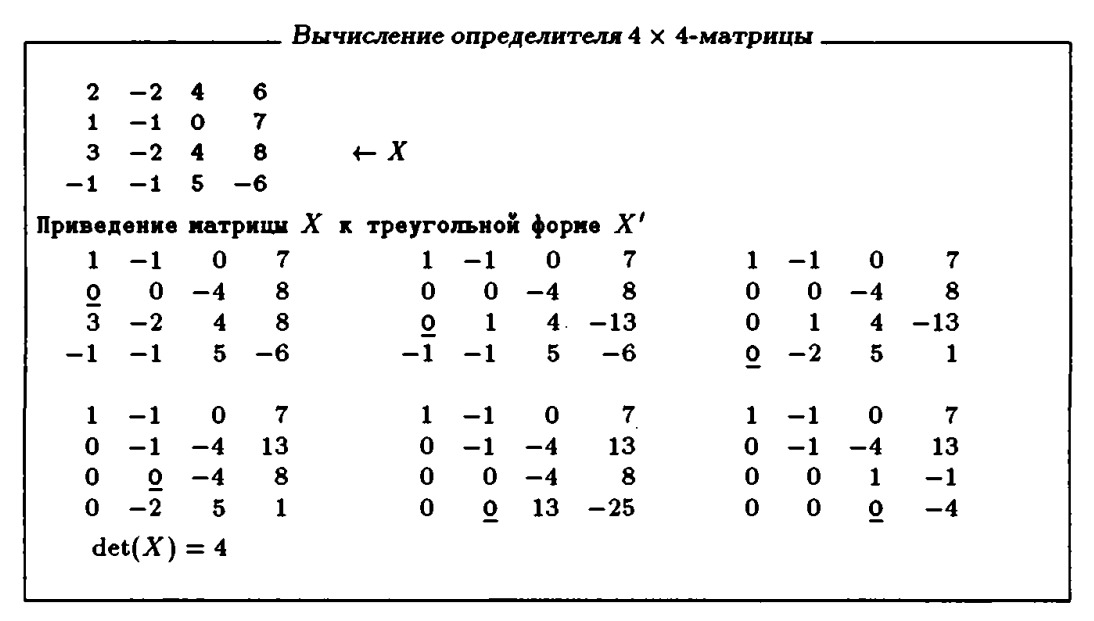
\includegraphics[width=1\linewidth]{316str}}
\end{figure}

Этот метод позволяет получить результаты с более разумным вре- \linebreak менем вычисления: на микрокалькуляторе типа AT время вычисления \linebreak определителя матрицы размеров $10 \times 10$ порядка 20 секунд (для на- \linebreak ивного метода было нужно более часа вычислений). Наконец, чтобы \linebreak убедиться в справедливости вычислений (никто не застрахован от оши-\linebreak
%317
\noindent бок), мы вычислили снова определители Майе!:  
$$h*(p)=h_1(p)=|\det (X_{ij})_{3 \le i, j \le (p-1)/2}|, X_{ij}=\lfloor{\frac{ij}{p}}\rfloor - \lfloor{\frac{(i-1)j}{p}}\rfloor,$$
для простого $p \le 47$ и сравнили полученные нами значения со значени- \linebreak ями, встречающимися в литературе. Эти определители имеют большое \linebreak значение в теории чисел. В действительности, существует целое поло- \linebreak жительное число, обозначаемое $h(p)$, которое измеряет степень неглав- \linebreak ности кольца $\mathbb{Z}[\sqrt[p]{1}]$ целых циклотомических чисел: $h(p)$ — число клас- \linebreak сов идеалов кольца $\mathbb{Z}[\sqrt[p]{1}]$. Сказать, что это кольцо — КГИ, равнозначно \linebreak тому, что $h(p) = 1$. Разумеется, можно разложить $h(p)$ в произведение \linebreak $h(p) = h_1(p)h_2(p)$ где $h_1(p)$ и $h_2(p)$ названы, соответственно, первым \linebreak и вторым множителем числа классов $\mathbb{Z}\sqrt[p]{1}$. Число $h_1(p)$, обозначаемое \linebreak также $h^*(p)$ и $h^-(p)$ (число $h_2(p)$ обозначается также $h^+(p)$), обладает \linebreak следующим фундаментальным свойством:
$$p \nmid h^*(p)\Longleftrightarrow p \nmid h(p),$$
$$p \nmid h^*(p) \Rightarrow \text{великая} \ll \text{ теорема } \gg \text{Ферма истинна для показателя } p,$$
указанная теорема утверждает, что уравнение $x^p + y^p = z^p$ не имеет \linebreak целых строго положительных решений для простых $p \ge 3$.
  
Интересующийся этим вопросом читатель может обратится к ра- \linebreak боте Рибенбойма $[153]$, в которой фигурирует таблица чисел $h^*(p)$ для \linebreak простых $p \le 163$, вычисленная вручную Куммером во второй поло- \linebreak вине 19-ого века. Здесь найдено простое число $p$, для которого $\mathbb{Z}[\sqrt[p]{1}]$ не \linebreak будет КГИ ($р = 23$), и простое нерегулярное число $p$, т.е. такое, что $p$ \linebreak делит $h^*(p)$ ($p = 37$). Эта таблица дает, в то же время, порядок размера \linebreak чисел $h^*(p)$: например, $h^*(149) = 3^2 \times 149 \times 512966338320040805461$.
\subsection{Модули без кручения конечного типа.}
\noindent Вот другое более абстрактное применение леммы исключения.

\begin{predl}
Пусть $M$ — $A$-модуль \textbf{конечного типа}, т.е. порожденный конеч- \linebreak ным числом образующих, и \textbf{без кручения)}(т.е. для $a \in A$, $x \in X$,\linebreak $ax=0 \Rightarrow a=0$ или $x=0$) над \textbf{КГИ} $A$. Обозначим через $\rho(M)$ мини- \linebreak мальное число элементов в системе образующих $M$. Тогда  
(i) любая порождающая $M$ система элементов, имеющая $\rho(M)$ эле- \linebreak ментов, свободна,  
(ii) в частности, $М$ свободен.  \newpage
%318
Отметим, что минимальная система образующих необязательно яв- \linebreak ляется системой с минимальным числом элементов. Рассмотрите, на- \linebreak пример, минимальную систему образующих $(2,3)$ в $\mathbb{Z}$.
\end{predl} 
\begin{lemma}
Пусть $A$ --- кольцо главных идеалов, $x_1, x_2, ..., x_n$ --- $n$ элементов \linebreak $A$ --- модуля $M$, $a_1, a_2, ..., a_n$ --- $n$ элементов кольца $А$. Тогда существуют \linebreak $x_1', х_2', ..., x_n'$ в $M$, удовлетворяющие условию:  
$$Ax_1 + Ax_2 + ... + Ax_n = Ax_1' + Ax_2' + ... + Ax_n' и a_1x_1 + a_2x_2 + ... + a_nx_n = dx_1',$$
$d \in A$ обозначает НОД элементов $a_1, a_2, ..., a_n$.
\end{lemma}
\begin{myproof}
В силу индукции достаточно рассмотреть лемму для $n=2$; по лем- \linebreak ме исключения существует матрица ${\left( \begin{array}{ccc}
\alpha & \beta \\
\gamma & \delta \\
\end{array} \right)} \in SL(2,A)$, удовлетворя- \linebreak ющая условию:  
$${\left( \begin{array}{ccc}
d & 0 \\
\end{array} \right)}{\left( \begin{array}{ccc}
\alpha & \beta \\
\gamma & \delta \\
\end{array} \right)}={\left( \begin{array}{ccc}
a_1 & a_2 \\
\end{array} \right)},$$
$d$ — НОД$(a_1, a_2)$. Достаточно определить $x_1', x_2' \in M$:
$${\left( \begin{array}{ccc}
x_1' \\
x_2' \\
\end{array} \right)}={\left( \begin{array}{ccc}
\alpha & \beta \\
\gamma & \delta \\
\end{array} \right)}{\left( \begin{array}{ccc}
x_1 \\
x_2 \\
\end{array} \right)}.$$
Это равенство можно преобразовать (матрица обратима), доказав, \linebreak что $Ax_1+ Ax_2= Ax_1' + Ax_2'$ . Тогда имеют место равенства:  
$$a_1x_1 + a_2x_2 = {\left( \begin{array}{ccc}
a_1 & a_2 \\
\end{array} \right)}{\left( \begin{array}{ccc}
x_1 \\
x_2 \\
\end{array} \right)} = {\left( \begin{array}{ccc}
a_1 a_2 \\
\end{array} \right)} {\left( \begin{array}{ccc}
\alpha & \beta \\
\gamma & \delta \\
\end{array} \right)}^{-1}{\left( \begin{array}{ccc}
x_1' \\
x_2 '\\
\end{array} \right)} = {\left( \begin{array}{ccc}
d & 0\\
\end{array} \right)} {\left( \begin{array}{ccc}
x_1' \\
x_2'\\
\end{array} \right)} = dx_1',$$
что и требовалось доказать.
\end{myproof}
\noindent\textbf{Доказательство предложения 9}


Пусть $\{x_1, x_2,..., x_n\}$ порождающее подмножество модуля $M$, со- \linebreak стоящее из $n = \rho (M)$ элементов. Рассмотрим соотношение зависимо- \linebreak сти $a_1x_1 + a_2x_2 + ... +a_nx_n = 0$. Докажем, что все $a_i$ нулевые, и, как \linebreak следствие, что $\{x_1, x_2, ..., x_n\}$ --- базис $М$.  \newpage
%319
В силу предыдущей леммы существует семейство образующих \linebreak $\{x_1', x_2',..., x_n'\}$ в $M$ такое, что $dx_1' = 0$, $d$ --- наибольший общий дели- \linebreak тель $a_1, a_2, ..., a_n$. Здесь $x_1'$ \textbf{не нуль}, иначе семейство $x_2', x_3', ..., x_n'\}$ \linebreak было бы семейством образующих, имеющим строго меньше, чем $\rho (M)$ \linebreak элементов. То, что $M$ без кручения, влечет, что $d$ --- нуль, и, как след- \linebreak ствие, что все $a_i$ нулевые. Это доказывает (i)  и (ii).

\section{Нормальная форма подгруппы группы $\mathbb{Z^n}$}
\noindent Сейчас мы продемонстрируем более общие результаты,чем сформули- \linebreak рованные (для $\mathbb{Z^2}$) во введении к этой главе и касающиеся представле- \linebreak ния в каноническом виде подгрупп $\mathbb{Z^n}$.

\subsection{Исследование подгруппы $n\mathbb{Z} \times m\mathbb{Z}$ группы $\mathbb{Z^2}$}
\noindent Целью наших действий в этом частном случае является стремление \linebreak объяснить читателю некоторые составные части теории инвариантных \linebreak множителей. Во введении мы установили существование изоморфизма \linebreak между абелевыми группами $\mathbb{Z_n} \times \mathbb{Z_m}$ и $\mathbb{Z_{n \wedge m}} \times \mathbb{Z_{n \vee m}}$; оно базировалось \linebreak на разложении чисел $n$ и $m$ в произведение простых множителей, и в \linebreak явном виде представлено на было; сделаем это сейчас.
  
Основная идея состоит в том, чтобы сконцентрироваться на поло- \linebreak жении подгруппы $n\mathbb{Z} \times m\mathbb{Z}$ в $\mathbb{Z} \times \mathbb{Z}$, забыв ненадолго про произведение \linebreak $\mathbb{Z_n} \times \mathbb{Z_m}$. Важно убедиться, что группа $n\mathbb{Z} \times m\mathbb{Z}$ изучена в окружающем \linebreak пространстве $\mathbb{Z}\times \mathbb{Z}$. Чтобы понять этот основной нюанс, рассмотрим \linebreak две подгруппы $2\mathbb{Z} \times \mathbb{Z}$ и $3\mathbb{Z} \times \mathbb{Z}$ группы $\mathbb{Z}^2$. Эти две подгруппы, очевид- \linebreak но, изоморфны, но между тем, не существует изоморфизма $\mathbb{Z}^2$ на себя,\linebreak переводящего первую группу во вторую (почему?).
  
Следующий результат, применимый к произведению двух цикличе- \linebreak ских групп, является более общим и более конструктивным, чем резуль- \linebreak тат, приведенный во введении.  
\begin{predl}
Пусть $n$ и $m$ два целых числа, $d = n \wedge m$, $p = n \vee m$. Существует \linebreak квадратная матрица $L$ порядка 2 с целыми коэффициентами и с опре- \linebreak делителем 1, представляющая автоморфизм $\mathbb{Z} \times \mathbb{Z}$ и удовлетворяющая \linebreak следующему условию: $L(n\mathbb{Z} \times m\mathbb{Z}) = d\mathbb{Z} \times p\mathbb{Z}$. Кроме того, эта матрица \linebreak легко выражается в явном виде.
\end{predl}
\newpage
%320
\begin{myproof}
Отметим еще раз, что построение такой матрицы основано на со- \linebreak отношении Безу. Можно предположить, что одно из двух целых \linebreak чисел $n$ или $m$ не нулевое; пусть $d = un +vm$ --- отношение Безу \linebreak и положим $\tilde{n} = n/d$ и $\tilde{m} = m/d$ при условии, что $u\tilde{n} + v\tilde{m} = 1$,\linebreak $\tilde{n}m = \tilde{m}n = p$. Матрица $L = {\left( \begin{array}{ccc}
u & v \\
-\tilde{m} & \tilde{n} \\
\end{array} \right)}$ , которая уже фигури- \linebreak ровала в лемме исключения, — искомая: ее определитель, конечно, \linebreak равен 1, и можно легко показать, что $(d, 0)$ и $(0, p)$ принадлежат \linebreak $L(n\mathbb{Z} \times m\mathbb{Z})$, т.е. что $d\mathbb{Z} \times p\mathbb{Z} \subset L(n\mathbb{Z} \times m\mathbb{Z})$. Можно также по- \linebreak казать, что $L(n\mathbb{Z} \times m\mathbb{Z})\subset d\mathbb{Z} \times p\mathbb{Z}$. Это доказывает равенство в \linebreak формулировке предложения.
\end{myproof}
\begin{sled}
В соответствии с предыдущими обозначениями, матриц \linebreak $L = {\left( \begin{array}{ccc}
u & v \\
-\tilde{m} & \tilde{n} \\
\end{array} \right)}$ и обратная матрица $L^{-1} = {\left( \begin{array}{ccc}
\tilde{n} & -v \\
\tilde{m} & u \\
\end{array} \right)}$ индуцируют \linebreak изоморфизмы $\overline{L}$ из $\mathbb{Z}_n \times \mathbb{Z}_m$ в $\mathbb{Z}_d \times \mathbb{Z}_p$ и $\overline{L^{-1}}$ из $\mathbb{Z}_d \times\mathbb{Z}_p$ в $\mathbb{Z}_n \times \mathbb{Z}_m$ \linebreak (каждая, соответственно). 
Можно еще улучшить предыдущие результаты:  
$${\left( \begin{array}{ccc}
d & 0 \\
0 & p \\
\end{array} \right)} = L {\left( \begin{array}{ccc}
n & -vp \\
m & up \\
\end{array} \right)} = L {\left( \begin{array}{ccc}
n & 0 \\
0 & m \\
\end{array} \right)}{\left( \begin{array}{ccc}
1 & -v\tilde{m} \\
1 & u\tilde{n} \\
\end{array} \right)} = {\left( \begin{array}{ccc}
n & 0 \\
0 & m \\
\end{array} \right)}R,$$
где  $R = {\left( \begin{array}{ccc}
1 & -v\tilde{m} \\
1 & u\tilde{n} \\
\end{array} \right)}$ --- $2 \times 2$ - матрица с целыми коэффициентами и с \linebreak определителем 1. Как следствие имеем: 
\end{sled}
\begin{predl}
Используя предыдущие обозначения, можно выразить в явном виде \linebreak $2 \times 2$ - матрицы $R$ и $L$ с определителями 1, удовлетворяющие условию: 
${\left( \begin{array}{ccc}
d & 0 \\
0 & p \\
\end{array} \right)} =  L{\left( \begin{array}{ccc}
n & 0 \\
0 & m \\
\end{array} \right)}R, где d делит p.$
\end{predl}
\begin{mynotice}
Раньше считали этот результат более сильным, чем \linebreak предыдущие. В действительности же, интерпретируя $n \mathbb{Z} \times m \mathbb{Z}$ \linebreak как образ диагональной матрицы ${\left( \begin{array}{ccc}
n & 0 \\
0 & m \\
\end{array} \right)}$ получаем, что равенство \linebreak матриц, объявленное в предложении 13, влечет равенство   
$$L(n\mathbb{Z} \times m\mathbb{Z}) = d\mathbb{Z} \times p\mathbb{Z}$$
\end{mynotice}
\newpage
%321
Действительно, этот последний результат является частным случа- \linebreak ем следующей более общей теоремы, которая будет доказана позже и \linebreak которая ведет к классификации абелевых групп конечного типа.  
\begin{thm}
Пусть дана квадратная $q \times q$-матрица $А$ с целыми элементами. Мож- \linebreak но предъявить две $q \times q$-матрицы $L$ и $R$ с целыми элементами и с опре- \linebreak делителем 1 такие, что $B = LAR$ будет диагональной матрицей и вы- \linebreak полняется условие:  
$$b_{11}|b_{22}, b_{22}|b_{33}, ..., b_{q-1 q-1}|b_{qq},$$
и, как следствие, переходя к частному, $\mathbb{Z}^q / ImA \simeq \mathbb{Z}_{b_{11}} \times \mathbb{Z}_{b_{22}} \times ... \times \mathbb{Z}_{b_{qq}}.$
\end{thm}
\subsection{Изучение подгруппы $a_1\mathbb{Z} \times ... \times a_n\mathbb{Z}$ группы $\mathbb{Z^n}$}
\noindent Этот параграф, посвященный изучению конечного произведения \linebreak $\mathbb{Z_{a_1}} \times \mathbb{Z_{a_2}} \times ... \times \mathbb{Z_{a_n}}$ циклических групп, должен позволить читате- \linebreak лю близко познакомиться с понятием инвариантных множителей: как \linebreak и в случае $n = 2$ в предыдущем разделе, мы будем изучать положение подгруппы $\mathbb{Z_{a_1}} \times \mathbb{Z_{a_2}} \times ... \times \mathbb{Z_{a_n}}$ в группе $\mathbb{Z^n}$.

\begin{determ}
\
 \begin{description} \item[(i)]  Две последовательности целых чисел $(a_1, a_2, ..., a_n)$ и \linebreak $(b_1, b_2, ..., b_m)$ называются \textbf{эквивалентными}, если существует изо- \linebreak морфизм $\varphi : \mathbb{Z^n} \to \mathbb{Z^m}$, переводящий подгруппу $\mathbb{Z_{a_1}} \times \mathbb{Z_{a_2}} \times ... \times \mathbb{Z_{a_n}}$ в \linebreak подгруппу $\mathbb{Z_{b_1}} \times \mathbb{Z_{b_2}} \times ... \times \mathbb{Z_{b_m}}$ (это незамедлительно влечет равенство \linebreak $n = m$, как мы увидим в следствии 19).  
\item[(ii)] Последовательность целых чисел $a_1, a_2, ..., a_n$ называется \textbf{нор-} \linebreak \textbf{мализованной}, если $a_1 | a_2 | a_3 | ... | a_{n-1} | a_n$.   
Если две последовательности целых чисел $(a_1, a_2, ..., a_n)$ и \linebreak $(b_1, b_2, ..., b_m)$ эквивалентны, то $n = m$ и --- что больше всего нас инте-\linebreak ресует, --- факторгруппы $\mathbb{Z_{a_1}} \times \mathbb{Z_{a_2}} \times ... \times \mathbb{Z_{a_n}}$ и $\mathbb{Z_{b_1}} \times \mathbb{Z_{b_2}} \times ... \times \mathbb{Z_{b_m}}$ изо- \linebreak морфны. Достаточно перейти к частным для изоморфизма из пункта \linebreak \item[(i)] . Заметим, что при переходе к частным, каждое $a_i$, равное 1 или -1, \linebreak соответствует тривиальному фактору $\mathbb{Z} / \mathbb{Z}$, который можно опустить.

\end{description} 
\end{determ}
\emph{\textbf{(16) Предложение.}}

Существует алгоритм, который, будучи применен к последователь- \linebreak ности целых чисел $a_1, a_2, ..., a_n$, строит \textbf{нормализованную} последо- \linebreak вательность $b_1, b_2, ..., b_n$, \textbf{эквивалентную} исходной.  \newpage
%322
В частности, для конечного произведения $\mathbb{Z_{a_1}} \times \mathbb{Z_{a_2}} \times ... \times \mathbb{Z_{a_n}}$ ци- \linebreak клических групп изоморфизм с произведением $\mathbb{Z_{b_1}} \times \mathbb{Z_{b_2}} \times ... \times \mathbb{Z_{b_m}}$, где \linebreak $b_i$ --- целые числа, отличные от 1 и -1, и $b_i$ делят $b_{i+1}$, может быть \linebreak выражен в явном виде.

\begin{lstlisting}[mathescape=true]

  $b \in \mathbb{Z}^n$ Normaliser $(a \in \mathbb{Z}^n)$
  $b = (b_1, b_2, ..., b_n) \gets (a_1, a_2, ..., a_n)=a;$
  for($i = 1$; $i < n-1$; $++i$)
      for ($j=i+1$; $j<n$; $++j$)
          $(b_i, b_j) \gets (b_i ) \wedge b_j, b_i \vee b_j);$
      

  return $(b_1, b_2, ..., b_n);$

\end{lstlisting}
\begin{myproof}\linebreak
Это доказательство основано на программной обработке, можно \linebreak также обратиться к упражнению 18. Уточним сейчас, что исполь- \linebreak зуемый метод не основан на разложении целых чисел $a_i$ в произве- \linebreak дение простых сомножителей: единственное, что используется, --- \linebreak это наибольший общий делитель $\wedge$ и наименьшее общее кратное $\vee$.\linebreak Пусть даны два индекса $i < j$; из результатов предыдущего раздела \linebreak понятно, что:  
$$(a_1,...,a_i,...,a_j,...,a_n) \sim (a_1,...,a_i \wedge a_j,...,a_i \vee a_j,...,a_n),$$
$\sim$ символизирует эквивалентность последовательностей, фигуриру-\linebreak ющих в определении 15.  

\noindent Назовем $E_{ij}$ операцию, которая состоит в замене первой из этих \linebreak последовательностей на вторую. Тогда ясно, что, если выполнить \linebreak последовательно операции $E_{12}, E_{13}, E_{14}, ..., E_{1n}$, то получится по- \linebreak следовательность $a'$, эквивалентная исходной и удовлетворяющая,\linebreak кроме того, условиям делимости $a_1'|a_2', a_1'|a_3', ..., a_1'|a_n'$ (дей- \linebreak ствительно, $a_1'$ --- НОД элементов исходной последовательности).\linebreak Затем можно применить к подпоследовательности $(a_2', a_3',..., a_n')$\linebreak операции $E_{23}, E_{24}, ..., E_{2n}$, после чего получим, очевидно, \linebreak эквивалентную подпоследовательность, удовлетворяющую условию \linebreak $a_2''|a_3'', a_2''|a_4'', ..., a_2''|a_n''$ и, к тому же, $a_1'|a_2''$ (потому что $a_2''$ \linebreak является НОД $a_i'$, каждое из которых делится на $a_1'$).  \newpage
%323

\noindent Применяя $n-1$ раз этот процесс (последней операцией будет \linebreak $E_{n, n-1}$), получаем последовательность, эквивалентную начальной и \linebreak нормализованную. Алгоритм 2 нормализации вытекает из этих рас- \linebreak суждений.
\end{myproof}
Интерпретация на языке Ада, которая приводится ниже, основа- \linebreak на не на функции, как в алгоритме, описанном выше, а на процедуре. \linebreak Эта процедура имеет только один параметр типа in out. Цель это-\linebreak го алгоритма, кроме нормализации последовательностей целых чисел, \linebreak построить след всего процесса нормализации.
\begin{lstlisting}[mathescape=true]
 #include<stdio.h>
 #include<stdlib.h>
 int n;   
 void Trace_Normalization (b : Module_Representation) {
    for(i=$b'First$; $i<b'Last-1$; ++i){
        for($j=i+1$; $j<b'Last$; ++j){
            b(i):=GCD_bi_bj;
            if (GCD_bi_bj = 0) 
            {
                b(j):=0; 
            } 
            else 
            {    
                b(j):=(bi/GCD_bi_bj)^*bj;

        
  void Get (a: Module_Representation){
      for(k=0; k<a; ++k){
          scanf("%d",&(a(k)));
      }
      while( true) {
          printf("Длина представления : ");
          scanf("d", &n);
          a= Module_Representation (1 .. n);
          printf("представление : ");
          scanf("%d", &a);
          printf("Данное представление : ");
          printf("%d", a);
          printf("%d", b);
          printf("Приведение : ");
          Trance_Normalization (a);
          if (Data_Error => NULL){
              break;          
\end{lstlisting}
\newpage
Вот только несколько примеров применения предыдущей прог- \linebreak раммы. 
\begin{figure}[h]
\center{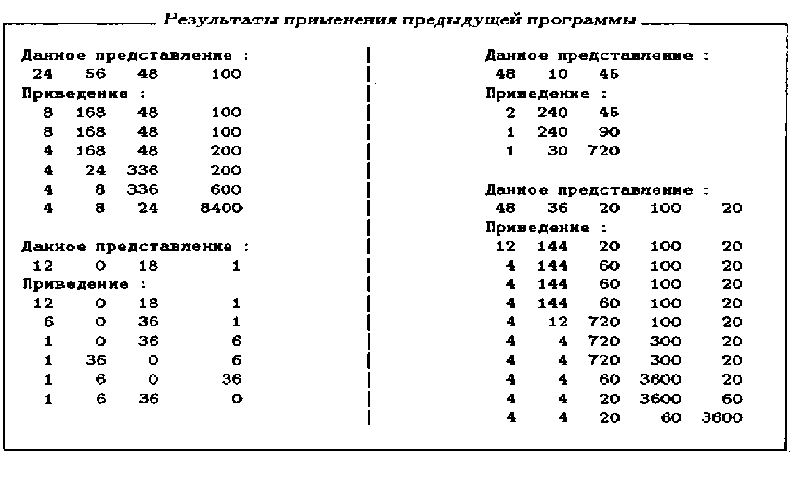
\includegraphics[width=1\linewidth]{324str}}
\end{figure}
\noindent А теперь выделим все основные понятия теории инвариантных множителей: матрицы с целыми коэффициентами, подгруппы образов,\linebreak факторгруппы $\mathbb{Z}^g/ImA$, нормализованные формы...  
\subsection{Единственность нормального разложения}
\noindent В предыдущем разделе мы показали, что любое произведение $\mathbb{Z}_n \times \mathbb{Z}_m$ \linebreak можно всегда заменить, используя изоморфизм, другим произведением \linebreak $\mathbb{Z}_{n'} \times \mathbb{Z}_{m'}$, где $n'$ делит $m'$. Но среди всех способов записи $\mathbb{Z}_n \times \mathbb{Z}_m$ в \linebreak виде произведения двух циклических групп лучший, когда $n$ делит $m$. 
\\
\\
\textbf{Пример}
\\

Рассмотрим группу, имеющую 48 элементов, представленную в виде \linebreak произведения двух циклических групп, $\Omega = \mathbb{Z}_{2} \times \mathbb{Z}_{24}$ . Числа 24 и 2 можно \linebreak найти, \textbf{зная только структуру группы $\Omega$}. Действительно, число 24 \linebreak получено следующим образом:   
 $$24\mathbb{Z} = \{ q \in \mathbb{Z} \text{ удовлетворяющие условию } qx = 0 , \forall x \in \Omega\} =$$ $$
= \{g \in \mathbb{Z},\text{ удовлетворяющие условию } q\Omega = \{0\}\}.$$

Это можно записать (выражение в фигурных скобках является опреде- \linebreak лением слова аннулятор): $24\mathbb{Z}$ = аннулятор($\Omega$). Что касается числа 2, \linebreak оно находится из равенства $2 \times 24$ = порядок($\Omega$). Таким образом, абеле- \linebreak ва группа ${\Omega}' = \mathbb{Z}_4 \times \mathbb{Z}_{12}$ имеет порядок в точности 48, но ее аннулятор --- \linebreak $12\mathbb{Z}$, поэтому ${\Omega}'$ не может быть изоморфна группе $\Omega = \mathbb{Z}_2 \times \mathbb{Z}_{24}$ (две \linebreak изоморфные группы имеют равные аннуляторы). 
\begin{predl}

Пусть $n, m, n'$ и $m'$ --- четыре элемента из $\mathbb{Z}$ такие, что $n | m$,\linebreak $n' | m'$ и $\mathbb{Z}_n \times \mathbb{Z}_m \simeq \mathbb{Z}_{n'} \times \mathbb{Z}_{m'}$. Тогда $n = \pm n'$, $m = \pm m'$; это можно \linebreak также записать в виде $n\mathbb{Z} = n'\mathbb{Z}$ и $m\mathbb{Z} = m' \mathbb{Z}$. 

На этой стадии, вдохновленный предыдущим примером\linebreak ($\Omega = \mathbb{Z}_2 \times \mathbb{Z}_{24}$, читатель может доказать теорему единственности, по \linebreak крайней мере в случае, когда $n, m, n', m'$ не нули. Заметим однако, что \linebreak этот результат единственности говорит также, что $\mathbb{Z} \times \mathbb{Z}$ не изоморфна \linebreak $\mathbb{Z}$, но это уже другая история. 

Сейчас мы докажем теорему единственности, имеющую очень широ- \linebreak кий спектр действия. Технические методы отличны от методов, исполь- \linebreak зуемых в частном случае в предыдущем примере: вместо аннуляторов \linebreak мы будем использовать минимальное число образующих для модулей \linebreak конечного типа.
%326
\end{predl}
\begin{thm}[единственности.]

$A$ обозначает \textbf{коммутативное} унитарное кольцо. Пусть \linebreak $I_1, I_2, ..., I_p$ и $J_1, J_2, ..., J_p$ --- \textbf{собственные} идеалы кольца $A$, удо- \linebreak влетворяющие условию: 
$$I_p \subset I_{p-1}\subset ... \subset I_1, J_p \subset J_{q-1}\subset ... \subset J_1$$
$$и A/I_1 \times A/I_2 \times ... \times A/I_p \simeq A/J_1 \times A/J_2 \times ... \times A/J_p$$
Тогда $p = q$ и $I_i = J_i$ для $i = 1, 2, ...$ 
\end{thm}
\begin{sled}
Пусть A — коммутативное унитарное кольцо; если $p$ и $q$ таковы, \linebreak что $A^p$ изоморфно $A^q$, тогда $p = q$ (непосредственное применение пре- \linebreak дыдущей теоремы в случае, когда идеалы нулевые). 

Чтобы доказать теорему 18, необходимо использовать несколько \linebreak лемм. Но прежде всего несколько комментариев о предпосылках тео- \linebreak ремы.
\end{sled}
\begin{mynotice} То, что все идеалы будут предполагаться отличны- \linebreak ми от А, позволяет избежать появления тривиальных множителей \linebreak $A/A$; кроме того, условие на цепи идеалов является необходимым, \linebreak как это показывает пример $\mathbb{Z}_2 \times \mathbb{Z}_3 \simeq \mathbb{Z}_6$. 

Если идеалы главные, $I_1 = (a_1), I_2 = (a_2), ...,$\linebreak $I_p = (a_p)$, то условие на цепи эквивалентно отношениям дели- \linebreak мости:
$$a_1 | a_2 | a_3 ... a_{p-1} | a_p.$$ 

Основное кольцо предполагается коммутативным и фунда- \linebreak ментальным. В действительности существуют не коммутативные \linebreak унитарные кольца А, такие, что $A \simeq A^2$ как A-модули. Рассмо- \linebreak трим, например, векторное $\mathbb{Q}$-пространство конечных последова- \linebreak тельностей из $\mathbb{N}$ в $\mathbb{Q}$ и кольцо А эндоморфизмов из $\mathbb{Q}^{\mathbb{N}}$. Пусть $u$ \linebreak и $v$ — два элемента из A, определенные их действием на канони-\linebreak ческом базисе: 
$$u(e_{2n}) = e_n, u(e_{2n+1}) = 0, v(e_{2n}) = 0, v(e_{2n+1}) = e_n.$$
Тогда имеем: $A = Au \oplus Av$. Чтобы это доказать, достаточно рас- \linebreak смотреть отображения $U$ и $V$, отвечающие $u$ и $v$ соответственно, \linebreak такие, что $U(e_n) = e_{2n}$, $V(e_n) = e_{2n + 1}$, значит $uU = vV = Id$.\linebreak Нетрудно видеть, что в этом случае $Id = Uu + Vv$.
\end{mynotice}
\begin{lemma}
Пусть дан A-модуль М конечного типа, обозначим через $\rho(M)$ наи- \linebreak меньшее число образующих из М.  
%327
Пусть $I_1 \supset I_2 \supset ... \supset I_p$ --- цепь собственных идеалов в А. Тогда \linebreak $\rho(A/I_1 \times A/I_2 \times ... \times A/I_p) = p.$
\end{lemma}
\begin{myproof}
Теорема Крулля утверждает существование максимального идеала \linebreak $\mathcal{M}$, содержащего собственный идеал $I_1$
 (если $A = \mathbb{Z}$ и $I_1 = (a_1)$, то \linebreak этот идеал --- $(q)$, где $q$ — простой делитель $a_1$). Этот идеал будет \linebreak самым большим в цепи. Применим тогда сюръективное отображе- \linebreak ние:

$$\pi:A/I_1 \times A/I_2 \times ... \times A/I_p \to {(A/ \mathcal{M})}^p,$$
которое является произведением канонических отображений \linebreak $A/I_i \to A/ \mathcal{M}$. Если $S$ --- система образующих в $A/I_1 \times A/I_2 \times$ \linebreak $... \times A/I_p$, то $\pi(S)$ --- система образующих векторного $A/\mathcal{M}$- \linebreak пространства ${(A/\mathcal{M})}^p$ и, следовательно, $card \; S \; \ge \; card \; \pi(S) \; \ge$ \linebreak $dim{(A/ \mathcal{M})}^p = p$. Любая система образующих в $A/I_1 \times A_/I_2 \times ... \times$ \linebreak $A/I_p$ содержит по крайней мере $p$ элементов. К тому же, семейство \linebreak $e_1 = (\overline{1}, 0, ..., 0), e_2 = (0, \overline{1}, 0, ..., 0), ..., e_p = (0, ..., 0, \overline{1})$ --- система \linebreak образующих в $A/I_1 \times A/I_2 \times ... \times A/I_p$, имеющая ровно $p$ элементов.\linebreak Следовательно,  
$$\rho(A/I_1 \times A/I_2 \times ... \times A/I_p) = p.$$
\end{myproof}
\begin{lemma}
Пусть $I$ — идеал в $A$ и $b \in A$. Существует канонический изоморфизм \linebreak $bA/I \simeq A/I^b$, идеал $I^b$ определяется как $I^b = \{x \in A | bx \in I\}.$ 
\end{lemma}
\begin{myproof}
Отображение $A \to bA/I$, которое элементу $x \in A$ ставит в соот- \linebreak ветствие элемент $b\overline{x} \in bA/I$ является сюръективным с ядром $I^b$ и \linebreak индуцирует изоморфизм между A-модулями $bA/I$ и $A/I^b$.\par
\end{myproof}
\textbf{Доказательство теоремы 18}

Пусть $P = A/I_1 \times A/I_2 \times ... \times a/I_p$ и $Q = A/J_1 \times A/J_2 \times ... \times A/J_q$. \linebreak В силу леммы 20, $p = \rho(P)$.\par

Докажем равенство $I_1 = \{b \in A | \rho(bP) \le p - 1\}$. По предыдущей \linebreak лемме имеет место равенство:\par
$$bP \simeq A/{I_1}^b \times A/{I_2}^b \times ... \times A/{I_p}^b, \text{где } {I_1}^b \supset {I_2}^b \subset ... \subset {I_p}^b.$$


	\lhead{328}
	\rhead{III-2 \ \ \ \  Нормальная форма подгруппы группы ${\mathbb Z}^{n}$}
	
	\noindent
	В силу леммы 20, если $I^{b}_{1} \neq A$, то $\rho (bP) = p$. В тоже время $\rho (bP)$ являет-\linebreak
	ся минимальным кардинальным числом. Если $I^{b}_{1} = A$, то $\rho (bP) \leqslant p - 1$.\linebreak
	Следовательно,
	$$\rho (bP) \leqslant p - 1 \Longleftrightarrow I^{b}_{1} = A \Longleftrightarrow b \in I_{1}.$$
	Аналогично можно показать, что $I_{k} = \{b \in A \ | \ \rho (bP) \leqslant p - k \}$ для\linebreak
	$1 \leqslant k \leqslant p$.
	
	Итак, мы определили $p, I_{1}, I_{2}, \ldots, I_{p}$, и это определение {\bf внутрен-}\linebreak
	{\bf нее}, зависит от $A$-модуля $P$: $P$ изоморфно $Q$, тогда $p = q$ и $I_{i} = J_{i}$.
	
	Приведем сейчас два следствия из теоремы единственности. Отме-\linebreak
	тим различие между посылками: в первом случае ищут изиморфизм\linebreak
	между частными, и $a_{i}$ и $b_{i}$ предполагаются необратимыми; во втором\linebreak
	$-$ речь идет об изоморфизме в окружающей среде, $a_{i}$ и $b_{j}$ могут быть\linebreak
	обратимыми.
	
	\noindent
	{\bf (22) Следствие.}
	
	Пусть $A$ $-$ {\it коммутативное унитарное кольцо}. Если $a_{1}, a_{2}, \ldots, a_{p}$ и\linebreak
	$b_{1, b_{2}, \ldots, b_{q}}$ {\bf необратимые} элементы, удовлетворяющие условиям:
	$$a_{1} |a_{2}|\ldots |a_{p - 1}|a_{p} \ \ \text{и} \ \ b_{1} |b_{2}|\ldots |b_{q - 1}|b_{q},$$
	$$A/(a_{1}) \times A/(a_{2}) \times \ldots \times A/(a_{p}) \ \simeq \ A/(b_{1}) \times A/(b_{2}) \times \ldots \times A/(b_{q}),$$
	то $p = q$ и элементы $a_{i}$ и $b_{i}$ ассоциированы. В частности, если коль-\linebreak
	цо $A$ без делителей нуля, то элементы $a_{i}$ и $b_{i}$ равны с точностью до\linebreak
	обратимого сомножителя.
	
	\noindent
	{\bf (23) Следствие.}
	
	$A$ обозначает опять коммутативное унитарное кольцо. Пусть\linebreak
	$a_{1}, a_{2}, \ldots, a_{p}$ и $b_{1}, b_{2}, \ldots, b_{q}$ - элементы, удовлетворяющие условиям:\linebreak
	$$a_{1} |a_{2}|\ldots |a_{p - 1}|a_{p} \ \ \text{и} \ \ b_{1} |b_{2}|\ldots |b_{q - 1}|b_{q},$$
	$$\exists \varphi : a^{p} \xrightarrow{\simeq} A^{q}, \ \ \varphi (a_{1}A \times a_{2}A \times \ldots \times a_{p}A) = b_{1}A \times b_{2}A \times \ldots \times b_{q}A.$$
	Тогда $p = q$ и элементы $a_{i}$ и $b_{i}$ ассоциированы (т.е. $a_{i}A = b_{i}A$), что\linebreak
	влечет равенство:
	$$a_{1}A \times a_{2}A \times \ldots \times a_{p}A = b_{1}A \times b_{2}A \times \ldots \times b_{q}A.$$
	Если кольцо $A$ без делителей нуля, то элементы $a_{i}$ и $b_{i}$ равны с точно-\linebreak
	стью до обратимого.

	\pagebreak
	
	\lhead{III-3 \ \ \ \  Вычисление образа и ядра матрицы}
	\rhead{329}

	\noindent
	{\bf Доказательство.}
	
	\begin{tabular}{|p{12.5cm}}
	\noindent
	Так как $A^{p}$ изоморфно $A^{q}$ (обозначим изоморфизм $\varphi$), то $p = q$.\linebreak
	Кроме того, изоморфизм $\varphi$ индуцирует, будучи перенесен на част-\linebreak
	ное, изоморфизм:
	$$A/(a_{1}) \times A/(a_{2}) \times \ldots \times A/(a_{p}) \ \simeq \ A/(b_{1}) \times A/(b_{2}) \times \ldots \times A/(b_{q}).$$
	Нельзя прямо применить теорему 18, так как некоторые из $a_{i}$ или\linebreak
	$b_{j}$ могут быть обратимыми. Определим $n$ и $m$ следующим образом:
	$$1 \leqslant i \leqslant n \Longleftrightarrow  (a_{i}) = A \ \text{и} \ 1 \leqslant j \leqslant m \Longleftrightarrow  (b_{j}) = A.$$
	Тогда имеет место изоморфизм:
	$$A/a_{n + 1} \times A/a_{n + 2} \times \ldots \times A/a_{p}$$
	$$A/b_{m + 1} \times A/b_{m + 2} \times \ldots \times A/b_{q}.$$
	Откула получаем $p - n = q - m$, следовательно $n = m$ (потому, что\linebreak
	$p = q$) и $(a_{i}) = (b_{i})$ для $i > n$. Так как $a_{i}$ и $b_{i}$ с индексами, меньшими\linebreak
	или равными $n$, обратимы, то для всех $i (a_{i}) = (b_{i})$.
	\end{tabular}
	
	\noindent
	{\Large {\bf 3 Вычисление образа и ядра матрицы}}
	
	\noindent
	В следующем разделе мы изучим некоторые вычислительные методы,\linebreak
	применяемые к матрицам с целыми элементами. Действительно, толь-\linebreak
	ко одно арифметическое свойство кольца чисел исполбзуется для\linebreak
	этих вычислений, поэтому везде можно заменитьь слова {\it с целыми эле-\linebreak
	ментами} на слова {\it с элементами в КГИ}. Однако, эти вычислительные\linebreak
	методы могут быть применимы, только если в рассматриваемом кольце\linebreak
	известны коэффициенты Безу.
	
	\noindent
	{\large {\bf 3.1 Ступенчатые матрицы}}
	
	\noindent
	Пусть $X$ $n\times m$-матрица с целыми элементами. Прежде всего мы постро-\linebreak
	им базис в  Im$X$ - подмодуле из ${\mathbb Z}^{n}$, порожденном $m$ столбцами матри-\linebreak
	цы $X$. Основная идея этого метода состоит в замене $n\times m$-матрицы\linebreak
	$X$ другой матрицей $X'$, более простой, чем $X$, и эквивалентной справа\linebreak
	матрице $X$ в смысле, определенном ниже.\newline
	
	\noindent
	{\bf (24) Определение.}
	
	{\it Пусть $X$ и $X'$ $-$ две матрицы с целыми элементами}. Они называю-\linebreak

	\pagebreak
	
	\lhead{330}
	\rhead{III-3 \ \ \ \  Вычисление образа и ядра матрицы}
	
	\noindent
	тся {\bf эквивалентными справа} {\it тогда и только тогда, когда существу-\linebreak
	ет обратимая матрица $R$, удовлетворяющая условию $X' = XR$. Это\linebreak
	равенсто определяет, естесственно, отношение эквивалентности}.\linebreak

	Две эквивалентные справа матрицы $X$ и $X'$ имеют один и тот же\linebreak
	образ: действительно, отношение между функциями $f' = fg$, в котором\linebreak
	$g$ обратимо, влечет, что $f$ и $f'$ имеют один образ. Следовательно, если\linebreak
	знать образ одной из этих матриц, то тогда изестен и образ другой\linebreak
	матрицы. Следовательно, необходимо рассмотреть класс матриц, образ\linebreak
	которых легко вычисляется. Матрицы, называемые ступенчатыми в\linebreak
	столбцах, образуют такой класс.
	
	\noindent
	{\bf (25) Определения.}
	
	{\it {\bf Высотой} вектора $x$ из $A^{n}$ ($n$ - произвольное кольцо) называется\linebreak
	целое число $n - i$, где $i$ самое большое из чисел, для которых $x_{j} = 0$ при\linebreak
	$1 \leqslant j \leqslant i$, т.е. $(0, 0, \ldots, 0, x_{i + 1}, x_{i + 2}, \ldots, x_{n})$ при $x_{i + 1} \neq 0$. Термин {\it $\ll$ вы-\linebreak
	сота$\gg$} происходит из того, что это понятие применяют для столбцов\linebreak
	матрицы. Нулевой вектор, и только он, имеет высоту 0.
	
	Матрица X размеров $n \times m$ со столбцами $X_{1}, X_{2}, \ldots, X_{m}$ назы-\linebreak
	вается {\bf ступенчатой в столбцах}, если высота ее столбцов является\linebreak
	убывающей, т.е. существует $k$ такое, что:
	$$h(X_{1}) > h(X_{2}) > \ldots > h(X_{k}) > 0 \ \text{и} \ X_{k + 1} = X_{k + 2} = \ldots X_{m} = 0,$$
	где $h(X_{i})$ обозначает высоту вектора $X_{i}$.}
	
	\noindent
	{\large {\bf 3.2 Вычисление образа матрицы}}
	
	\noindent
	Ступенчатые матрицы имеют простую структуру и обладают несколь-\linebreak
	кими элементарными свойствами, которые широко используются.
	
	\noindent
	{\bf (26) Свойства} (ступенчатых матриц).
	
	{\it Пусть $X$ $-$ ступенчатая матрица над {\bf кольцом без делителей\linebreak
	нуля.}}

	$(i)$ {\it Ненулевые столбцы матрицы $X$ образуют базис пространства,\linebreak
	порожденного столбцами.}

	$(ii)$ {\it Векторы $(e_{i})_{i > k}$, отвечающие нулевым столбцам $(X_{i})_{i > k}$, обра-\linebreak
	зуют базис ядра матрицы $X$.}
	
	Следующая теорема имеет важное значение: она показывает, что\linebreak
	любая матрица с целыми коэффициентами (в общем случае - с коэф-\linebreak
	фициентами в КГИ) может быть преобразована в ступенчатую мат-\linebreak
	рицу.
	
	\pagebreak
	
	\lhead{III-3.2 \ \ \ \  Вычисление образа матрицы}
	\rhead{331}
	
	\noindent
	{\bf (27) Теорема.}
	
	$(i)$ {\it Существует алгоритм, который, будучи применен к матрице $X$\linebreak
	размеров $n\times m$ с целыми коэффициентами, дает обратимое справа пре-\linebreak
	образование, которое превращает матрицу $X$ в ступенчатую матрицу\linebreak
	$X'$. Более точно, этот алгоритм, примененный к $X$, дает пару $(X', R),$\linebreak
	где $X'$ - ступенчатая $n\times m$-матрица, $R$ - $m\times m$-матрица, принад-\linebreak
	лежащая $SL_{m}(\mathbb Z)$ и удовлетворяющая условию $X' = XR$. В этом случае\linebreak
	говорят, что $X'$} {\bf специально эквивалентна справа} {\it матрице $X$, \it что-\linebreak
	бы подчеркнуть существование правой матрицы перехода с} {\bf определи-\linebreak
	телем 1.}
	
	$(ii)$ {\it Результат остается справедливым, если кольцо целых чисел за-\linebreak
	менить на} {\bf КГИ}, {\it в котором имеется алгоритм, позволяющий вычи-\linebreak
	слить коэффициенты Безу. Если основное кольцо предполагается толь-\linebreak
	ко КГИ, то матрицы $R$ и $X'$ существуют независимо от того, можем\linebreak
	мы их представить в явном виде или нет.}
	
	Эта теорема, доказательство которой сопровождается алгоритмом,\linebreak
	имеет следствие <<абстрактной>> природы.
	
	\noindent
	{\bf (28) Следствие.}
	
	$(i)$ {\it Существует алгоритм, который будучи применен к $m$ векторам\linebreak
	из ${\mathbb Z}^{n}$, строит базис подмодуля в ${\mathbb Z}^{n}$, порожденного этими $m$ векторами.
	
	$(ii)$ Пусть $A$ }$-$ {\bf КГИ}; {\it любой подмодуль $A^{n}$ имеет базис, образо-\linebreak
	ванный самое большое из $n$ векторов. В частности, над кольцом глав-\linebreak
	ных идеалов любой подмодуль} {\bf свободного модуля конечного типа}\linebreak
	{\it является свободным конечного типа.}
	
		\fbox{%
		\parbox{10cm}{%
				{\footnotesize\definecolor{light-gray}{rgb}{0.8,0.8,0.8}
					\colorbox{light-gray}{$X'\in M_{nm}, X'_1, X'_2, ...,$ обозначают столбцы матрицы $X'$}\newline
				$X' \leftarrow X; j \leftarrow 1;$\newline
				for ($i = 0; i == n; i++$) \{\newline
				${\ \ \ }$if ($j == m$) \{\newline
				${\ \ \ \ \ \ }$break;\newline
				${\ \ \ }$\}\newline
				${\ \ \ }$for ($k = j + 1; k == m; k += 1$) \{\newline
				${\ \ \ \ \ \ }$\definecolor{light-gray}{rgb}{0.8,0.8,0.8}
				\colorbox{light-gray}{Вычислить ${\scriptsize \begin{pmatrix} \alpha & \gamma \\ \beta & \delta \end{pmatrix}_{jk}}$, удовлетворяющую условиям:}\newline
				${\ \ \ \ \ \ \ \ \ }$\definecolor{light-gray}{rgb}{0.8,0.8,0.8}
				\colorbox{light-gray}{ $\gamma X'_{ij} + \delta X'_{ik} = 0$ и $\alpha \delta - \beta \gamma = 1$}\newline
				${\ \ \ \ \ \ }$$(X'_j, X'_k) \leftarrow (\alpha X'_j + \beta X'_k, \gamma X'_j + \delta X'_k)$;\newline
				${\ \ \ }$\}\newline
				${\ \ \ }$if ($X'(i, j) \neq 0$) \{\newline
				${\ \ \ \ \ \ }$$j \leftarrow j + 1$;\newline
				${\ \ \ }$\}\newline
				\}\newline
				\definecolor{light-gray}{rgb}{0.8,0.8,0.8}
				\colorbox{light-gray}{$X' = XR$, где $R - $матрица с определителем 1. Она не вычислена.}}}}

	{\bf Алгоритм 3.} Приведение матрицы $X$ к ступенчатому\newline
	${\ \ \ \ \ \ \ \ \ \ \ \ \ \ \ \ \ \ \ \ \ \ \ \ \ \ \ \ \ \ \ \ \ \ \ \ \ \ \ }$ в столбцах виду 
	
	\pagebreak
	
	\lhead{332}
	\rhead{III-3 \ \ \ \  Вычисление образа и ядра матрицы}
	
	\noindent
	{\bf Доказательство} (следствия).

	\begin{tabular}{|p{12.5cm}}
	$(i)$ является частным случаем предыдущей теоремы, если рассмо-\linebreak
	треть матрицу, образованную данными $m$ векторами.\linebreak
	Чтобы доказать $(ii)$, рассмотрим подмодуль $M$ кольца $A^n$. Так как\linebreak
	$A^{n}$ - нётерово, то подмодуль $M$ имеет конечное число образую-\linebreak
	щих (обобщение модулей предложения 17 раздела II-2.4, посвящен-\linebreak
	ного свойству конечности идеалов нётерово кольца). Тогда можно\linebreak
	применить пункт $(i)$.
	\end{tabular}
	
	\noindent
	{\bf Неконструктивное доказательство}
	
	Докажем по индукции, что любой подмодуль $E$ кольца $A^{n}$ свободен\linebreak
	с базисом, состоящим из меньшего или равного $n$ числа элементов.
	
	Если $n = 1$, то $E$ - идеал в $A$, следовательно, $E$ имеет вид $Aa$, и\linebreak
	$\{a\}$ - базис $E$ (исключая, может быть, случай $a = 0$, для которого $\emptyset$\linebreak
	будет базисом $E$).
	
	Возьмем $n\geqslant 2$ и пусть $\pi_{n}:A^{n} \ \textrightarrow \ A$ - координатная функция\linebreak
	на $e_n$ - последнем векторе канонического базиса. Если $\pi_{n}(E) = 0$, то\linebreak
	$E\subset A^{n - 1}$ и  имеет (предположение индукции) базис $\{f_1, f_2, \ldots, f_m\}$ для\linebreak
	$m\leqslant n - 1$. Если $\pi_{n}(E) \neq 0$, то $E$ является идеалом $Aa$ кольца $A$ с $a \neq 0$.\linebreak
	Пусть $x \ in E$ и $\pi_{n}(x) = a$. Докажем тогда, что
	
	$$(E \cap A^{n - 1}) \oplus Ax = E \ \ \ \ \ \ \ \ \ \ \ \ \ \ \ (2)$$
	Сумма прямая, потому что, если $A \in E \cap A^{n - 1} \cap Ax$, то $y = \lambda x$ и\linebreak
	$\pi_{n}(y) = 0$. Отсюда $\lambda = 0$, затем $y = 0$. Сумма равна $E$, так как, если для\linebreak
	$y \in E$ взять разложение $y = y' + \lambda x$, то получим $\pi_{n}(y) = \lambda a$, что опре-\linebreak
	деляет $\lambda$ (по предположению $\pi_{n}(y) \in Aa$). Если положить $y' = y - \lambda x$,\linebreak
	то получим $y' \ in E \cap A^{n - 1}$.
	
	По индукции подмодуль $E \cap A^{n - 1}$ кольца $A^{n - 1}$ имеет базис\linebreak
	$\{f_1, f_2, \ldots, f_m\}$ при $m \leqslant n - 1$. Равенство (2) доказывает, что\linebreak
	$\{f_1, f_2, \ldots, f_m, x\}$ - базис $E$.
	
	В последнем пункте предыдущего следствия можно убрать условие\linebreak
	конечности, что приводит к следующему предложению, доказанному в\linebreak
	упражнении 16.
	
	\noindent
	{\bf (29) Предложение.}
	
	{\it Над кольцом главных идеалов любой подмодуль свободного модуля\linebreak
	свободен.}
	
	\pagebreak
	
	\lhead{III-3.2 \ \ \ \  Вычисление образа матрицы}
	\rhead{333}
	
	\noindent
	{\bf Доказательство теоремы 27}
	
	Покажем для начала как вычисляют $X'$; вычисление $R$ может быть\linebreak
	получено, как частный случай этого метода.
	
	Пусть $X'$ - $n\times n$-матрица, определенная по $X$. Ее столбцы обо-\linebreak
	значают через $X'_{1}, X'_{2}, \ldots, X'_{m}$. Благодаря лемме 6 об исключениях, на\linebreak
	столбцах $X'$ можно реализовать операцию:
	$$(X'_1, X'_2) \textleftarrow (\alpha X'_1 + \beta X'_2, \gamma X'_1 + \delta X'_2)$$
	$$\ \ \ \ \ \ \ \ \ \ \ \ \ \ \ \ \ \ \ \ \ \ \ \ \ \ \ \ \ \ \ \ \ \text{при} \ \alpha\delta-\beta\gamma = 1 \ \text{и} \ \gamma X'_{11} + \delta X'_{12} = 0.$$
	С обозначениями из раздела 1 эту операцию можно еще записать в виде:
	$$(X'_1, X'_2) \textleftarrow (X'_1, X'_2) \begin{pmatrix} \alpha & \gamma \\ \beta & \delta \end{pmatrix}_{12}.$$
	Эта операция производит к умножению справа матрицы $X'$ на матрицу\linebreak
	из $SL_{m}(\mathbb Z)$ и обнуляет $X'_{12}$. Таким же образом обнуляются элементы в\linebreak
	$X'_{12}, X'_{13}, \ldots, X'_{1m}$.
	
	При итераци метода представляются два случая:
	
	\begin{itemize}
	\item $X'_{11} \neq 0$. Тогда приводят к ступенчатому виду (по индукции) под-\linebreak
	матрицу $X'(2..n, 2..m)$, образованную $n - 1$ последними строками\linebreak
	и $m - 1$ последними столбцами.
	
	\item $X'_{11} = 0$. Тогда приводят к ступенчатому виду (по индукции) под-\linebreak
	матрицу $X'(2..n, 1..m)$, состоящую из $n - 1$ послеедних строк и\linebreak
	$m$ столбцов.
	\end{itemize}
	
	В обоих случаях результирующая матрица $X'$ будет ступенчатой.\linebreak
	Существование правой матрицы перехода $R$ приводит к тому, что ка-\linebreak
	ждая операция в действительности является умножением справа на эле-\linebreak
	ментарную матрицу.
	\begin{flushright}$\blacksquare$\end{flushright}
	{\ \ \ }Итак, можно дать более простой алгоритм, реализующий преобра-\linebreak
	зование матрицы $X$ в ступенчатую матрицу $X'$, специально эквивалент-\linebreak
	ную справа исходной матрице. Получение правой матрицы перехода $R$,\linebreak
	{\bf использующее только этот алгоритм}, будет объяснено ниже.\linebreak
	Чтобы лучше понять алгоритм 3, нужно отметить, что на данном\linebreak
	{\small
	\begin{minipage}[t]{80mm}\parindent=2em
		\noindent
		этапе выбирают индекс строки $i$ и ин-\linebreak
		декс столбца $j$ и пытаются обнулить все\linebreak
		элементы строки $i$ с индексом $k > j$.\linebreak
		Рассмотрим этот процесс на примере.\linebreak
		В этой матрице $a_{11}$ и $a_{32}$ {\bf не нули}, знач-\linebreak
		ки . обозначают произвольные элемен-\linebreak
		ты, а $\bullet$ - расположение начального мо-
	\end{minipage}
	\hfill
	\begin{minipage}[t]{50mm}
	\[ \bordermatrix{
		& & & \stackrel{j}{\textdownarrow} & & \stackrel{k}{\textdownarrow} & \cr
		& a_{11} & 0 & 0 & 0 & 0 & 0 \cr
		& . & 0 & 0 & 0 & 0 & 0 \cr
		& . & a_{32} & 0 & 0 & 0 & 0 \cr
		& . & . & 0 & 0 & 0 & 0 \cr
		i\textrightarrow  & . & . & \bullet & 0 & \ast & . \cr
	    & . & . & . & . & . & . \cr}
	\]
	\end{minipage}}

	\pagebreak
	
	\lhead{334}
	\rhead{III-3 \ \ \ \  Вычисление образа и ядра матрицы}
	
	\noindent
	мента (осевой столбец). Пытаются обнулить элемент $\ast$ (т.е. элемент в\linebreak
	строке $i$ и столбце $j$).
	
	\noindent
	{\bf Пример приведения к ступенчатому виду}
	
	Вот конкретный пример применения программы, иллюстрирующий\linebreak
	этапы приведения к ступенчатому виду матрицы размеров $4\times 3$. Приво-\linebreak
	дится каждый этап, в котором обнуляемый коэффициент еще не нуль.\linebreak
	Запись \underline{0} обозначает, что данный коэффициент {\it стал нулем на этом\linebreak
	этапе.}
	$$\begin{pmatrix} 6 & 15 & 10 \\ 12 & 0 & 10 \\ -12 & 30 & 0 \\ 18 & 15 & 20\end{pmatrix}, \begin{pmatrix} 3 & \underline{0} & 10 \\ -24 & -60 & 10 \\ 54 & 120 & 0 \\ -21 & -60 & 20\end{pmatrix},$$
	$$\begin{pmatrix} 1 & 0 & \underline{0} \\ 82 & -60 & 270 \\ -162 & 120 & -540 \\ 83 & -60 & 270\end{pmatrix}, \begin{pmatrix} 1 & 0 & 0 \\ 83 & 30 & \underline{0} \\ -162 & -60 & 0 \\ 83 & 30 & 0\end{pmatrix}$$
	
	Пусть $F$ - подпространство из ${\mathbb Z}^4$, порожденное 3 столбцами матрицы\linebreak
	$X$. Процесс приведения к ступенчатому виду из $X$ в $X'$ дает базис $F$.\linebreak
	Действительно, два первых столбца ступенчатой матрицы $X'$ образу-\linebreak
	ет базис $ImX'$, а значит, $F = ImX = ImX'$. Читателю предлагается\linebreak
	решить упражнение 12, в котором сообщается, что хотя $F$ имеет раз-\linebreak
	мерность 2, свободная система $\{X_1, X_2\}$ из $F$ не образует базис $F$ и не\linebreak
	может быть дополнена до базиса $F$.
	
	\noindent
	{\bf (30) Предупреждение.}
	
	{\it Приведем несколько основных классических результатов линейной\linebreak
	алгебры для векторных пространств.
	
	$(i)$ В ${\mathbb Z}^n$ в общем случае нельзя найти базис системы образующих.
	
	$(ii)$ Свободная система из $n$ векторов в ${\mathbb Z}^n$ не имеет никакого отно-\linebreak
	шения к построению базиса в ${\mathbb Z}^n$.
	
	$(iii)$ Дополнить свободную систему ${\mathbb Z}^n$ до базиса ${\mathbb Z}^n$, вообще говоря\linebreak
	невозможно.}

	Посмотрим сейчас, насколько это возможно в процессе приведения\linebreak
	к ступенчатому виду $X \rightarrow X' = XR$, как вычислить матрицу пере-\linebreak
	хода $R$. Достаточно взять переменную $R$ матричного типа размеров\linebreak
	$n\times m$, пока равную единичной, и произвести над ней те же элементар-\linebreak
	ные умножения справа, что и над $X'$. Практически процесс состоит\linebreak
	
	\pagebreak
	
	\lhead{III-3.2 \ \ \ \  Вычисление образа матрицы}
	\rhead{335}
	
	\noindent
	в построении новой матрицы. Приписывая к матрице $X$ {\it снизу} единич-\linebreak
	ную $n\times m$-матрицу, применим к этой $(n + m) \times m$-матрице алгоритм\linebreak
	приведения к ступенчатому виду по столбцам, помня, что достаточ-\linebreak
	но преобразовать к ступенчатому виду только верхнюю часть. Если\linebreak
	обозначить через $X'$ переменную, представляющую $n\times m$-подматрицу,\linebreak
	образованную из $n$ первых строк (т.е. первых строк) и через $R$ - пе-\linebreak
	ременную, представляющую подматрицу размеров $m\times m$, состоящую\linebreak
	из $m$ последних строк (т.е. нижних строк), то соотношение\linebreak
	$$XR = X', \ \ \ \ \ R \in SL_{m}(A),$$
	остается истинным на каждом шаге (обе части этого равенства умно-\linebreak
	жены справа на одну и ту же элементарнуюматрицу из $SL_{m}(A)$). Итак,\linebreak
	это соотношение остается истинным до конца алгоритма приведения к\linebreak
	ступенчатому виду и позволяет вычислить, таким образом, в явном\linebreak
	виде матрицу перехода $R$.
	
	\begin{flushleft}
	\hangindent=1cm \hangafter=0 \noindent
	{\small {\bf Замечание.}${\ \ \ \ \ \ \ }$Отметим, что в силу соотношения $X' = XR$ воз-\linebreak
		можно получить выражение векторов $X'_j$, векторов-столбцов ма-\linebreak
		трицы \  $X'$ \ в зависимости от векторов \ $X_j$, \ столбцов матрицы \ $X$.\linebreak
		Чтобы выразить \ $X_j$ через \ $X'_j$, достаточно умножить на \ $R^{-1}$ обе\linebreak
		части \ равенства, \ что возможно сделать с помощью \ алгоритма.\linebreak
		Можно также построить базис, исходя и з системы образующих,\linebreak
		и выразить в явном виде элемент базиса в этой \ системе образу-\linebreak
		ющих и наоборот.}
	\end{flushleft}
	
	\noindent
	{\bf Пример приведения к ступенчатому виду (продолжение)}
	
	Приведем пример, показывающий получение правой матрицы пере-\linebreak
	хода. Как обычно, показан каждый этап обнуления элемента; это обну-\linebreak
	ление будет обозначаться через подчеркнутый ноль \underline{0}:
	$$\begin{pmatrix} 6 & 15 & 10 \\ 12 & 0 & 10 \\ -12 & 30 & 0 \\ 18 & 15 & 20 \\ 1 & 0 & 0 \\ 0 & 1 & 0 \\ 0 & 0 & 1\end{pmatrix}\begin{pmatrix} 3 & \underline{0} & 10 \\ -24 & -60 & 10 \\ 54 & 120 & 0 \\ -21 & -60 & 20 \\ -2 & -5 & 0 \\ 1 & 2 & 0 \\ 0 & 0 & 1\end{pmatrix}$$
	
	\pagebreak
	
	\lhead{336}
	\rhead{III-3 \ \ \ \  Вычисление образа и ядра матрицы}
	
	$$\begin{pmatrix} 1 & 0 & \underline{0} \\ 82 & -60 & 270 \\ -162 & 120 & -540 \\ 83 & -60 & 270 \\ 6 & -5 & 20 \\ -3 & 2 & -10 \\ 1 & 0 & 3\end{pmatrix}\begin{pmatrix} 1 & 0 & 0 \\ 82 & 30 & \underline{0} \\ -162 & -60 & 0 \\ 83 & 30 & 0 \\ 6 & 0 & 5 \\ -3 & -2 & 2 \\ 1 & 3 & -6\end{pmatrix}.$$
	Сохраняя предыдущие обозначения, покажем на примере, как знание\linebreak
	матрицы $R$ помогает выразить векторы $X'_1, X'_2$ и  базиса $F$ в зависимо-\linebreak
	сти от начальной системы образующих $X_1, X_2, X_3$. Равенство $X' = XR$\linebreak
	влечет, в частности, равенства $X'_1 = XR_1$ и $X'_2 = XR_2$; они могут быть\linebreak
	записны в виде:
	$$X'_1 = 6X_1 - 3X_2 + X_3, X'_2 = -2X_2 + 3X_3.$$
	Отметим, что нулевое значение последней колонки влечет отношение\linebreak
	зависимости между $X_1, X_2$ и $X_3$:
	$5X_1 + 2X_2 - 6X_3 = 0.$
	Чтобы выразить $X_j$ через $X'_j$, достаточно знать матрицу $R^{-1}$. Эту\linebreak
	матрицу лгко получить, применив алгоритм приведения к ступенча-\linebreak
	тому виду. Действительно, $R$ получена, начиная с единичной матрицы,\linebreak
	умножением {\it справа} на элементарные матрицы {\scriptsize $\begin{pmatrix} \alpha & \gamma \\ \beta & \delta \end{pmatrix}_{jk}$}. Как следствие,\linebreak
	достаточно иметь квадратную матрицу $S$ того же размера, что и $R$, и\linebreak
	определенную как единичная. Затем подвергнуть ее умножению {\it слева},\linebreak
	на элементарные обратные к предшествующим, матрицы столько раз,\linebreak
	сколько подвергалась и матрца $R$. Отношение $RS = Id_m$ тогда оста-\linebreak
	нется инвариантным с начала и до конца алгоритма. Вэтом примере\linebreak
	мы получили матрицу $R^{-1}$ и выражение системы образующих в базисе\linebreak
	$$\begin{pmatrix} 6 & 15 & 10 \\ -16 & -41 & -27 \\ -7 & -18 & -12\end{pmatrix}, X_1 = 6X'_1 - 16X'_2$$
	$${\ \ \ \ \ \ \ \ \ \ \ \ \ \ \ \ \ \ \ \ \ \ \ \ \ \ \ \ \ \ \ \ \ \ \ \ \ \ \ \ \ \ }X_2 = 15X'_1 - 41X'_2, {\ \ \ }X_3 = 10X'_1 - 27X'_2.$$
	
	{\bf{\large3.3 Существование решения системы линейных\newline ${\ \ \ \ \ \ \ \ \ }$ уравнений}}
	
	Пусть $A$ - матрица размеров $n\times m$ с целыми элементами и $b$ - век-\linebreak
	тор с $n$ целыми компонентами, ассоциированные с системой линейных\linebreak
	уравнений $Ax = b$. Решить явно эту систему, значит:
	
	\pagebreak
	
	\lhead{III-3.3 \ \ \ \  Существование решения системы линейный уравнений}
	\rhead{337}
	
	{\bf1)} быть способным показать, имеет ли эта система одно решение и\linebreak
	при необходимости предъявить его,
	
	{\bf 2)} если система имеет решения, то найти их все, т.е. найти базис\linebreak
	ядра $KerA$.
	
	Общее решение системы линейных уравнений рассмотренно в разде-\linebreak
	ле 3.5. Здесь мы будем рассматривать только поиск решения. Сказать,\linebreak
	что система $Ax = b$ имеет решение, то же самое, что сказать, что век-\linebreak
	тор $b$ принадлежит образу $ImA$; найти решение - значит представить\linebreak
	вектор $b$ как линейную комбинацию столбцов $A$. Рассмотрим матри-\linebreak
	цу, полученную приписыванием справа к матрице $A$ столбца $b$. Итак,\linebreak
	достаточно изучить следующую задачу.
	
	{\bf 3)} Пусть дана матрица $X$ с $n$ строками и $m$ столбцами. Определить,\linebreak
	является ли последний столбец $X_m$ линейной комбинацией пред-\linebreak
	шествующих столбцов $X_1, X_2, \ldots, X_{m-1}$ и если да, то найти в\linebreak
	явном виде эту линейную комбинацию.
	
	\noindent
	{\bf (31) Теорема.}
	
	{\it Пусть $X$ - $n\times m$-матрица с целыми элементами. Обозначим через\linebreak
	$X'$ и $R$ две матрицы, полученные с помощью алгоритма приведения\linebreak
	к ступенчатому виду по столбцам ($R$ - квадратная матрица порядка\linebreak
	$m$ и обратима, $X' = XR$ \texttwelveudash ${\ }$ матрица, ступенчатая по столбцам). Если\linebreak
	$R = (r_{ij})$, следующие два свойства эквивалентны:
	
	a) последний столбец $X_m$ является линейной комбинацией столбцов\linebreak
	$X_1, X_2, \ldots, X_{m-1}$,
	
	b) столбец $X'_m$ нулевой и $r_{mm}$ обратимо.
	
	Тогда последняя строка матрицы $R$ будет $(0, 0, \ldots, 0, 0, 1)$, и имеет\linebreak
	место равенство:
	$$X_m = -(r_{1m}X_1 + r_{2m}X_2) + \ldots + r_{m - 1m}X_{m - 1},$$
	которое доказывает, что последний столбец $X_m$ матрицы $X$ является\linebreak
	линейной комбинацией предшествующих столбцов.\linebreak
	Эти результаты обобщаются, очевидно, на любое кольцо гланых\linebreak
	идеалов; сложностб вычисления зависит от сложности вычисления ко-\linebreak
	эффициентов Безу.}
	
	\noindent
	{\bf Доказательство.}
	
	\begin{tabular}{|p{12.5cm}}
	Докажем сначала импликацию $b \Rightarrow a$. Равенство $X' = XR$, интер-\linebreak
	претированное в терминах столбцов, описывается так:
	$$\textperiodcentered X'_j = r_{1j}X_1 + r_{2j}X_2 \ldots + r_{mj}X_m \ \  \text{для} \ \  1 \leqslant j \leqslant m.$$
	\end{tabular}
	
	\pagebreak
	
	\lhead{338}
	\rhead{III-3 \ \ \ \  Вычисление образа и ядра матрицы}
	
	\begin{tabular}{|p{12.5cm}}
	\noindent
	Если столбец $X'_m$ нулевой и если $e_{mm}$ обратимо, то из равенства,\linebreak
	приведенного выше, следует при $j = m$ выражение столбца $X_m$ в\linebreak
	виде линейной комбинации $X_1, X_2, \ldots, X_{m - 1}$.\linebreak
	Чтобы доказать обратную тмпликацию ${\bf a \Rightarrow b}$, нужно доказать,\linebreak
	что в любой момент в алгоритме приведения к ступенчатому виду\linebreak
	последняя строка матрицы $R$ всегда будет равна $(0, 0, \ldots, 0, 0, 1)$,\linebreak
	что можно еще записать в виде:
	$$R({\mathbb Z}^{n - 1}\times 0 = {\mathbb Z}^{n - 1}\times 0) \ \  \text{и} \ \ R(e_m) - e_m \in {\mathbb Z}^{n - 1}\times 0 \ \ \ \ \ \ \ \ \ \ \ \ \ \ \ \ \ \ \ \ \ (3)$$
	${\mathbb Z}^{n - 1}\times 0$ обозначает подпространство ${\mathbb Z}^{n - 1}$, образованное $n - 1$ пер-\linebreak
	выми векторами $(e_i)_{1 \leqslant i \leqslant n - 1}$ канонического базиса.\newline
	Это доказывается по индукции: сначала возбмем квадратную ма-\linebreak
	трицу $R$ единичной. На каждом этапе $R$ изменяется - умножается\linebreak
	на элементарные матрицы:
	$$R \ \longleftarrow R{\small \begin{pmatrix} \alpha & \gamma\\ \beta & \delta \end{pmatrix}_{jk}}$$
	Так как множество матриц, удовлетворяющих условию (3), образу-\linebreak
	ют подгруппу $GL_m(\mathbb Z)$, достаточно доказать, что матрица ${\scriptsize \begin{pmatrix} \alpha & \gamma\\ \beta & \delta \end{pmatrix}_{jk}}$\linebreak
	принадлежит этой подгруппе, что очевидно, если $k < m$.\linebreak
	Итак, интересен этап, для которого индексы осевых столбцов будут\linebreak
	$j$ и $m$. Достаточно доказать, что в этом случае $\beta = 0$ и $\delta = 1$.\linebreak
	Если $X'$ обозначает матричную переменную $XR$, то столбец $X'_m$\linebreak
	является линейной комбинацией предыдущих столбцов $X'_1, X'_2, \ldots$,\linebreak
	$X'_{m - 1}$. Действительно:
	$$X'_m \stackrel{\text{def}}{=} ZR(e_m)\in XR({\mathbb Z}^n) = X({\mathbb Z}^n) = X({\mathbb Z}^n \times 0)$$
	$${\ \ \ \ \ \ \ \ \ \ \ \ \ \ \ \ \ \ \ \ \ \ \ }= XR({\mathbb Z}^n \times 0) \stackrel{\text{def}}{=} X'({\mathbb Z}^n \times 0).$$
	Первое равенство верно, так как $R$ обратима. Второе - так как\linebreak
	$X_m = X(e_m)$ является по предположению линейной комбинацией\linebreak
	$X'_1, X'_2, \ldots, X'_{m - 1}$ и так как $R$ удовлетворяет условию (3).\linebreak
	Покажем, что $x'_{ij}$ делит $x'_{im}, i$ - индекс текущей строки. Рассмо-\linebreak
	трим отношение между столбцами:
	$$X'_m = \lambda_1 X'_1 + \lambda_2 X'_2 + \ldots + \lambda_j X'_j + \ldots + \lambda_{m - 1} X'_{m - 1} {\ \ \ \ \ \ \ \ \ \ \ \ \ \ \ \ \ \ \ \ (4)}$$
	Так как матрица $X'$ уже частично ступенчатая, то подматрица,\linebreak
	составленная из $i - 1$ первых строк, будет ступенчатой. Ненулевые\linebreak
	\end{tabular}
	
	\pagebreak
	
	\lhead{III-3.3 \ \ \ \  Существование решения системы линейный уравнений}
	\rhead{339}
	
	\begin{tabular}{|p{12.5cm}}
	\noindent
	столбцы этой подматрицы, т.е. столбцы с индексом $< j$, образу-\linebreak
	ют множество линейно независимых элементов и отношение (4),\linebreak
	ограниченное до $i - 1$ первых строк, образует нулевую линейную\linebreak
	комбинацию этой линейно независимой системы. Следовательно,\linebreak
	$\lambda_1 = \lambda_2 = \ldots = \lambda_{j - 1} = 0$. Элемент отношения (4), индекс стро-\linebreak
	ки которого $i$, описывается как: $x'_{im} = \lambda_i x'_{ij}$, что доказывает ука-\linebreak
	занное отношение делимости. Однако алгоритм оговаривает, что\linebreak
	в случае, когда $x'_{ij}$ делит $x'_{im}$, нужно выбрать элемент $\beta$ матрицы\linebreak
	${\scriptsize \begin{pmatrix} \alpha & \gamma\\ \beta & \delta \end{pmatrix}_{jm}}$ равным 0, а $\delta$ - равным 1.\linebreak
	То, что последний столбец $X'_m$ {\bf финальной} матрицы $X'$ будет нуле-\linebreak
	вым, доказывает, что этот столбец является линейной комбинацией\linebreak
	предыдущих столбцов и что $X'$ {\bf полностью ступенчата}.
	\end{tabular}
	
	\noindent
	{\bf Пример решения}
	
	Вот пример решения линейной системы, иллюстрирующий доказа-\linebreak
	тельство теоремы 31. Рассмотрим линейную систему $Ax = b$ с:\linebreak
	$$\begin{pmatrix} 3 & 2 & 3 & 4 \\ 1 & -2 & 1 & -1 \end{pmatrix} \ \ \text{и} \ \ \begin{pmatrix} -8 \\ -3 \end{pmatrix}.$$
	Приведем этапы процесса ступенчатости:
	$$\begin{pmatrix} 3 & 2 & 3 & 4 & -8 \\ 1 & -2 & 1 & -1 & -3 \end{pmatrix}, \begin{pmatrix} -1 & \underline{0} & 3 & 4 & -8 \\ -3 & 8 & 1 & -1 & -3 \end{pmatrix},$$
	$$\begin{pmatrix} -1 & 0 & \underline{0} & 4 & -8 \\ 3 & 8 & -8 & -1 & -3 \end{pmatrix}, \begin{pmatrix} -1 & 0 & 0 & \underline{0} & -8 \\ 3 & 8 & -8 & -13 & -3 \end{pmatrix},$$
	$$\begin{pmatrix} -1 & 0 & 0 & 0 & \underline{0} \\ -3 & 8 & -8 & -13 & 21 \end{pmatrix}, \begin{pmatrix} -1 & 0 & 0 & 0 & 0 \\ -3 & 8 & \underline{0} & -13 & 21 \end{pmatrix},$$
	$$\begin{pmatrix} -1 & 0 & 0 & 0 & 0 \\ -3 & 1 & 0 & \underline{0} & 21 \end{pmatrix}, \begin{pmatrix} -1 & 0 & 0 & 0 & 0 \\ -3 & 1 & 0 & 0 & \underline{0} \end{pmatrix}.$$
	Получена правая матрица перехода:
	$$\begin{pmatrix} -1 & -2 & -1 & -6 & 50 \\ 1 & -3 & 0 & -7 & 55 \\ 0 & 0 & 1 & 0 & 0 \\ 0 & 3 & 0 & 8 & -63 \\ 0 & 0 & 0 & 0 & 1\end{pmatrix}.$$
	Тогда заключаем, что вектор $x = (-50, -55, 0, 63)$ является частным\linebreak
	решением предложенной системы. 
	
	\pagebreak
	
	\lhead{340}
	\rhead{III-3 \ \ \ \  Вычисление образа и ядра матрицы}
	
	\noindent
	{\large {\bf 3.4 Вычисление ядра матрицы}}
	
	\noindent
	Ступенчатый вид матрицы позволяет также выразить ядро матрицы.
	
	\noindent
	{\bf (32) Предложение.}
	
	{\it $A$ обозначает здесь кольцо главных идеалов. Пусть $X \ \texttwelveudash \  n\times m$-\linebreak
	матрица с элементами в $A$ и $R$ - обратимая матрица порядка $m$ такая,\linebreak
	что $X' = XR$ будет ступенчатой по столбцам. Если $X'_{k + 1}, X'_{k + 2}, \ldots$,\linebreak
	$X'_{m}$ $\ \texttwelveudash \ $ нулевые столбцы матрицы $X'$, то:
	
	$(i)$ последние столбцы $R_{k + 1}, \ldots, R_{m}$ матрицы $R$ образуют базис\linebreak
	подпространства Ker$X$ кольца $A^m$,
	
	$(ii)$ $k$ первых столбцов матрицы $R$ образуют базис дополнения $S$ до\linebreak
	Ker$X$ в $A^m$:
	$$S = \bigoplus\limits_{i = 1}^k AR_i, KerX = \bigoplus\limits_{i = k + 1}^m AR_i \ \text{и} \ A^m = S \oplus KerX,$$
	$(iii)$ для $x \in A^m$ разложение $R^{-1}(x)$ в каноническом базисе будет\linebreak
	иметь вид: $R^{-1}(x) = \sum_{i = 1}^m \lambda_i (x)e_i$. Тогда $\sum_{i = 1}^k \lambda_i (x)R_i$ и $\sum_{i > k}^m \lambda_i (x)R_i$\linebreak
	будут компонентами $X$ в прямой сумме, описанной выше. Следователь-\linebreak
	но, $KerX$ {\bf выражает} прямое слагаемое в $A^m$.}
	
	\noindent
	{\bf Доказательство.}
	
	\begin{tabular}{|p{12.5cm}}
	Равенство $X' = XR$ доказывает для $x\in A^m$ эквивалентность $Rx\in$\linebreak
	$KerX \Longleftrightarrow x\in KerX'$ и, следовательно, $R(KerX') = KerX$. Ясно,\linebreak
	что $e_{k + 1}, e_{k + 2}, \ldots, e_{m}$ образует базис ядра $X'$. Остальную часть\linebreak
	предложения докажем ниже.
	\end{tabular}

	\noindent
	{\bf Пример}
	
	Проиллюстрируем это доказательство на примере матрицы разме-\linebreak
	ров $3\times 4$. Возьмем матрицу $X$, ее ступенчатую форму $X'$, матрицу $R$\linebreak
	перехода от $X$ к $X'$, удовлетворяющую условию $X' = XR$.
	$$X = \begin{pmatrix} 6 & 3 & 6 & 1 \\ 2 & 5 & 6 & -1 \\ 8 & 11 & 15 & -1 \end{pmatrix}, \ \ \ X' = \begin{pmatrix} 1 & 0 & 0 & 0 \\ -1 & -4 & 0 & 0 \\ -1 & -7 & 0 & 0 \end{pmatrix},$$
	$$R = \begin{pmatrix} 0 & 0 & 1 & 0 \\ 0 & -2 & 2 & 3 \\ 0 & 1 & -2 & -2 \\ 1 & 0 & 0 & 3 \end{pmatrix}.$$
	
	\pagebreak
	
	\lhead{III-3.3 \ \ \ \  Общее решение системы линейный уравнений}
	\rhead{341}
	
	Усли обозначить через $R_i$ столбцы $R$, то векторы $R_3$ и $R_4$, ко-\linebreak
	торые соответствуют нулевым столбцам матрицы $X'$, образуют базис\linebreak
	ядра матрицы $X$. Кроме того, имеется разложение ${\mathbb Z}^4$ в прямую сумму:\linebreak
	$${\mathbb Z}^4 = (\mathbb Z R_1\oplus \mathbb Z R_2) \oplus (\mathbb Z R_3\oplus \mathbb Z R_4) = (\mathbb Z R_1\oplus \mathbb Z R_2) \oplus \text{Ker}X,$$
	а знание матрицы $R^{-1}$ влечет разложение: $e_1 = (6R_1 - 2R_2) \oplus (R_3 - 2R_4),$\linebreak
	$e_2 = (6R_3 - 2R_2) \oplus (-R_4), e_3 = (6R_1 - 3R_2) \oplus (-2R_4), e_4 = (R_1) \oplus (0).$
	
	\noindent
	{\large {\bf 3.5 Общее решение систеы линейных уравнений}}
	
	\noindent
	В разделе 3.3. уже было определено, что значит решить линейную систе-\linebreak
	му с целыми коэффициентами $Ax = b$, где $x \in \mathbb Z^m$ и $b \in \mathbb Z^n$. Существо-\linebreak
	вание и поиск частного решения уже были рассмотрены в разделе 3.3.\linebreak
	В то же время, хорошо известно, что общее решение такой системы -\linebreak
	это сумма частного решения и общего решения однородной системы.\linebreak
	Однако ядро матрицы $A$ (множество однородных решений) было вы-\linebreak
	численно в предыдущем разделе. Итак, линейное уравнение, описанное\linebreak
	выше, полностью решено. Но нужно сделать замечание: ядро матрицы\linebreak
	$A$ может быть вычислено во время поиска частного решения, т.е. одно-\linebreak
	временно с процессом приведения к ступенчатому виду матрицы $A$, к\linebreak
	которой присоединен вектор-столбец $b$.
	
	\noindent
	{\bf (33) Предложение.}
	
	{\it Обозначим через $(A | b)$ матрицу, состоящую из матрицы $A$ и присо-\linebreak
	единенного к ней вектора $b$. Тогда $(A | b)$ будет линейным отображени-\linebreak
	ем из $\mathbb Z^m \times \mathbb Z \ \text{в} \ \mathbb Z^n$, которое $x, x_{m + 1}$ ставит в соответствие $Ax + bx_{m + 1}$.
	
	Пусть $(A' | b')$ - ступенчатая матрица, полученная с помощью ал-\linebreak
	горитма приведения к ступенчатому виду из раздела 3.2, примененного\linebreak
	к матрице $(A | b)$. $R$ - матрица перехода, удовлетворяющая условию\linebreak
	$(A | b)\times R = (A' | b')$ (эта матрица $R$ обратима и порядка $m + 1$).
	
	$(i)$ Система $Ax = b$ имеет решение тогда и только тогда, когда\linebreak
	последняя строка матрицы $R$ равна $(0, 0, \ldots, 0, 0, 1)$ и когда вектор $b'$\linebreak
	нулевой. Эти два условия гарантируют частное решение $-\overline{R}_{m + 1}$, где\linebreak
	$\overline{R}_{m + 1}$ - вектор, образованный $m$ первыми компонентами из $R_{m + 1}$.
	
	$(ii)$ Вэтом случае $A'$ - ступенчатая матрица, эквивалентная слева\linebreak
	матрице $A$. Пусть $k \in [1, m]$ такое, что нулевые столбцы матрицы $A$\linebreak
	имеют индексы $> k$. Тогда векторы $\overline{R}_{k + 1}, \overline{R}_{k + 2}, \ldots, \overline{R}_{m} \in \mathbb Z^m$ состоят из\linebreak
	$m$ первых компонент столбцов $R_{k + 1}, R_{k + 2}, \ldots, R_{m}$ образующих базис\linebreak
	$KerA$.}
	
	\pagebreak
	
	\lhead{342}
	\rhead{III-3 \ \ \ \  Вычисление образа и ядра матрицы}
	
	\noindent
	{\bf Доказательство.}
	
	\noindent
	\begin{tabular}{|p{12.5cm}}
	Пункт $(i)$ следует из теоремы 31. Тогда имеет место матричное\linebreak
	равенство:
	$$(A | b)\times R = (A' | b') = (A' | 0) \ \text{для} \ R = \left( \left.\frac{\overline{R}}{0 \ldots 0} \right| \frac{\overline{R}_{m + 1}}{1} \right),$$
	которое ведет к $A' = A\times \overline{R} \ \text{и} \ A\overline{R}_{m + 1} + b = 0$; это доказывает\linebreak
	пункт $(ii)$.
	\end{tabular}
	
	\noindent
	{\bf Пример}
	
	Проиллюстрируем данное доказательство примером, уже рассмо-\linebreak
	тренным в разделе 3.3. Речь идет о системе уравнений $3x_1 + 2x_2 + 3x_3 +$\linebreak
	$+ 4x_4 = -8\ \text{и} \ x_1 - 2x_2 + x_3 - x_4 = -3$. Приведем ступенчатую форму\linebreak
	$(A' | b')$ матрицы $(A | b)$ и матрицу перехода $R$ от $(A | b)$ к $(A' | b')$:
	$$(A' | b') = \begin{pmatrix} -1 & 0 & 0 & 0 & 0 \\ -3 & 1 & 0 & 0 & 0 \end{pmatrix},\ \ \  R = \begin{pmatrix} -1 & -2 & -1 & -6 & 50 \\ 1 & -3 & 0 & -7 & 55 \\ 0 & 0 & 1 & 0 & 0 \\ 0 & 3 & 0 & 8 & -63 \\ 0 & 0 & 0 & 0 & 1 \end{pmatrix}.$$
	\ \ \ Два основных пункта обеспечивают нулевое значение вектора $\b'$ и\linebreak
	то, что последняя строка матрицы $R$ равна $(0, 0, 0, 0, 1)$. Действительно,\linebreak
	если $x \ -$ вектор $(-50, -55, 0, 63)$, то соотношение $(A | b)\times R_5 = 0$ опи-\linebreak
	сывается в виде: $-Ax + r_{55}b = 0$. Следовательно, $x - $ частное решение\linebreak
	системы $Ax = b$. Кроме того, имеет место равенство $A\times\overline{R} = A'$, ма-\linebreak
	трица $\overline{R}$ будет подматрицей матрицы $R$, состоящей из 4 первых строк\linebreak
	и 4 первых столбцов матрицы $R$. Это матричное равенство имеет тот\linebreak
	смысл, что матрица $A'$ является ступенчатой формой матрицы $A$, и\linebreak
	$\overline{R}$ - правая матрица перехода. Векторы $\overline{R}_3$ и $\overline{R}_4$, соответствующие\linebreak
	нулевым столбцам матрицы $A'$, образуют базис $KerA$. Другими слова-\linebreak
	ми, $\overline{R}_3, \overline{R}_4$ образуют базис пространства однородных решений. Итак,\linebreak
	решения записываются в виде:
	$$x_1 = -50 - u - 6v, \ \ \ x_2 = -55 - 7v,$$
	$$ \ \ \ \ \ \ \ \ \ \ \ \ \ \ \ \ \ \ \ \ \ \ \ x_3 = u, x_4 = 63 + 8u \ \ \text{для} \ \ u, v \in \mathbb Z.$$
	
	\pagebreak
	
	\lhead{III-3.6 \ \ \ \  Ранг модулей}
	\rhead{343}
	
	\noindent
	{\large {\bf 3.6 Ранг модулей}}
	
	\noindent
	Вот несколько результатов, относящихся к рангу модулей, которые,\linebreak
	возможно, покажутся смешными для читателя, хорошо знающего те-\linebreak
	орию модулей над кольцом главных идеалов. Предупреждения, фигу-\linebreak
	рирующие в этих формулировках, оправдывают их присутствие здесь.\linebreak
	Первые результаты будут верны не только в кольцах главных идеалов,\linebreak
	а останутся истинным и в коммутативных кольцах: предположение о\linebreak
	том, что кольцо является кольцом главных идеалов, позволяет, однако,\linebreak
	доказать, что приведение к ступенчатому виду предоставляет возмож-\linebreak
	ность эффективного подхода.
	
	\noindent
	{\bf (34) Предложение.}
	
	{\it Два базиса свободного модуля $L$ конечного типа над {\bf коммутатив-\linebreak
	ным} кольцом $A$ имеют одно и тоже число элементов.}
	
	\noindent
	{\bf Доказательство.}
	
	\begin{tabular}{|p{12.5cm}}
	\noindent
	Обозначим через $p$ кардинальное число одного базиса и через $q \ - $\linebreak
	кардинальное число другого базиса. По определению базиса, три\linebreak
	$A$-модуля $L, A^p$ и $A^q$ изоморфны. В силу следствия 19 раздела 2.3\linebreak
	имеем: $p = q$, что и доказывает предложение.
	\end{tabular}
	
	\noindent
	{\bf (35) Определения.}
	
	{\it Если $(i)$ - свободный модуль конечного типа над {\bf коммутатив-\linebreak
	ным} кольцом $A$, то мощность какого-либо его базиса называется ран-\linebreak
	гом модуля $L$ и обозначается через $rang(L)$. В частности, ранг $A^n$ равен\linebreak
	$n$.
	
	$(ii)$ Если $M - A$-модуль конечного типа, то обозначим, как и в\linebreak
	лемме 20 раздела 2.3, через $\rho(M)$ наименьшее число образующих в $M$.}
	
	\noindent
	{\bf (36) Предложение.}
	
	{\it Пусть $A - $ {\bf коммутативное} кольцо. Семейство образующих в $A^n$,\linebreak
	состоящее из $n$ элементов, является базисом в $A^n$. Другими словами,\linebreak
	любая сюръекция модуля $A^n$ является изоморфизмом.}
	
	\noindent
	{\bf Доказательство.}
	
	\begin{tabular}{|p{13cm}}
	\noindent
	Напомним, что квадратная матрица $X$ порядка $n$ является обра-\linebreak
	тимой тогда и только тогда, когда ее определитель обратим; это\linebreak
	равенство в силу равенства $\det(XY) = \det(X)\det(Y)$. Используя это\linebreak
	равенство для матрицы $\widetilde{X}$, присоединенной к матрице $X$, транс-\linebreak
	понируем матрицу алгебраических дополенений матрицы $X: X\widetilde{X} = $\linebreak
	$\widetilde{X}X = \det(X) \text{Id}_n$.
	\end{tabular}
	
	\pagebreak
	
	\lhead{344}
	\rhead{III-3 \ \ \ \  Вычисление образа и ядра матрицы}
	
	\begin{tabular}{|p{12.5cm}}
	\noindent
	Пусть $X - n\times n$матрица, столбцы которой $X_1, X_2, \ldots, X_n$ явля-\linebreak
	ются $n$ векторами порождающими $A^n$. Рассмотрим сначала част-\linebreak
	ный случай $A = \mathbb Z$. Если $X' - $ступенчатая матрица, эквивалентная\linebreak
	справа матрице $X$, то ее столбцы порождают Im$X' = $Im$X = \mathbb Z^n$.\linebreak
	Как следствие, всякий столбец матрицы $X' -$ ненулевой. Матрица\linebreak
	$X' -$ ступенчатая, ее столбцы назависимы и образуют базис $\mathbb Z^n$;\linebreak
	тогда то же верно и для столбцов матрицы $X$. Эти рассуждения\linebreak
	применимы, очевидно, и к любому кольцу главных идеалов.\linebreak
	Рассмотрим Теперь случай произвольного коммутативного кольца.\linebreak
	Так как $X_i$ составляют систему образующих для $A^n$, то существу-\linebreak
	ет семейство $(Y_i) n$ векторов из $A^n$ такое, что $X(Y_i) = e_i$, где\linebreak
	множество $e_i$ обозначает канонический базис. Если $Y$ обозначает\linebreak
	матрицу, столбцами которой являются векторы $Y_1, Y_2, \ldots, Y_n$, то\linebreak
	$XY = \text{Id}_n$ и $\det(X)\det(Y) = 1$. Следовательно, матрица $X$ с обра-\linebreak
	тимым определителем обратима; ее столбцы образуют базис в $A^n$.
	\end{tabular}
	
	Внимание: этот результат не имеет аналогов для множества линейно\linebreak
	независимых элементов (см. пример и предупреждение 30 раздела 3.2).\linebreak
	В упражнении 6 доказан следующий результат.
	
	\noindent
	{\bf (37) Предложение.}
	
	{\it Если $A$ - коммутативное кольцо, то в $A^n n$ векторов свободны\linebreak
	тогда и только тогда, когда их определитель не является делителем\linebreak
	нуля. Другими словами,эндоморфизм $A^n$ инъективен тогда и только\linebreak
	тогда, когда его определитель не является делителем нуля.}
	
	\noindent
	{\bf (38) Предложение.}
	
	{\it Пусть $A$ - произвольное {\bf коммутативное} кольцо.
		
	$(i)$ Множество $n + 1$ векторов из $A^n$ всегда зависимо.
	
	$(ii)$ Множество $n - 1$ векторов из $A^n$ не порождает $A^n$.
	
	$(iii)$ Если модуль $M$ порожден $n$ векторами, то $n + 1$ векторов всегда\linebreak
	линейно зависимы; и еще, если $M$ содержит $m$ линейно независимых\linebreak
	векторов, то $M$ не может быть порожден $m - 1$ векторами.
	
	$(iv)$ Если $L$ - свободный подмодуль модуля конечного типа $M$, то\linebreak
	rang$(L) \leqslant \rho(M)$.
	
	$(v)$ В частности, если $M$ - свободный подмодуль конечного типа,\linebreak
	то rang$(M) \leqslant \rho(M)$.}
	
	\pagebreak
	
	\lhead{III-3.6 \ \ \ \  Ранг модулей}
	\rhead{345}
	
	\noindent
	{\bf Доказательство.}\newline
	\begin{tabular}{|p{13cm}}
	$(i)$ Классическое доказательство состоит в использовании внеш-\linebreak
	него вычисления. Но можно дать более простое доказательство,\linebreak
	имитирующее внешнее вычисление с помощью подопределителей\linebreak
	(упражнение 6). Приведем здесь доказательство в двух частных\linebreak
	случаях. Предположим, например, что $A$ без делителей нуля и по-\linebreak
	грузим $n + 1$ данных векторов в $K^n$, где $K$ - поле частных для $A$.\linebreak
	Элементарный результат линейной алгебры о векторных простран-\linebreak
	ствах дает нам нетривиальное соотношение с коэффициентами в $K$,\linebreak
	которое умножается на общий знаменатель и дает нетривиальное\linebreak
	отношение с коэффициентами в $A$.\newline
	Более простое доказательство над кольцом главных идеалов состо-\linebreak
	ит в использовании ступенчатости. Обозначим через $X$ матрицу с\linebreak
	$n$ строками и $n + 1$ столбцами, образованную $n + 1$ данными век-\linebreak
	торами, через $X' -$ ступенчатую матрицу, эквивалентную справа\linebreak
	матрице $X$, через $R -$ матрицу перехода порядка $n + 1$, обрати-\linebreak
	мую и такую, что $XR = X'$. Матрица $X'$ обладает строго большим\linebreak
	числом столбцом, чем строк. Но так как она ступенчатая, то ее\linebreak
	последний столбец нулевой. Равенство $XR_{n + 1} = 0$ ($R_{n + 1} -$ послед-\linebreak
	ний столбец матрицы $R$) дает {\it нетривиальное} сооьношение между\linebreak
	столбцами матрицы $X$.
	
	$(iii)$ Первая часть следует из $(i)$. Пусть $u -$ сюръекция из $A^n$\linebreak
	на $M$. Рассмотрим тогда $n + 1$ векторов $\mu_1, \mu_2, \ldots, \mu_{n + 1}$ моду-\linebreak
	ля $M$, порожденного $n$ векторами. Если $X_i \in A^n - $ прообраз $\mu_i$ для\linebreak
	$i = 1, 2, \ldots, n + 1$, то $X_i$ в количестве $n + 1$ находятся в $A^n$. Нетриви-\linebreak
	альное линейное соотношение сежду $X_i$ проектируется с помощью\linebreak
	$u$ в нтривиальное линейное соотношение между $\mu_i$.\linebreak
	
	Вторая часть пункта $(iii)$ - переформулировка первой, которая\linebreak
	влечет, в частности, пункт $(ii)$. Пункты $(iv)$ и $(v)$ являются непо-\linebreak
	средственными следствиями из предыдущих пунктов.\linebreak
	Дополнительное замечание: метод приведения к ступенчатому виду\linebreak
	дает явное доказательство пункта $(ii)$, предъявляя вектор канони-\linebreak
	ческого базиса, не принадлежащего пространству, порожденному\linebreak
	$n - 1$ данными векторами из $A^n$. Действительно, рассмотрим ма-\linebreak
	трицу $n$, образованную этими $n - 1$ векторами, и ступенчатую ма-\linebreak
	трицу $X'$, эквивалентную справа матрице $X$. Матрица $X'$ имеет\linebreak
	$n$ строк, $n - 1$ столбцов и тот же образ, что и матрица $X$. Если\linebreak
	ни один из диагональных элементов матрицы $X'$ не нуль, то $e_n$ не\linebreak
	принадлежит образу $X'$, и, следовательно, $e_n \notin$Im$X$. Напротив,\linebreak
	если $X'$ имеет нулевой диагональный элемент, то выберем из таких
	\end{tabular}
	
	\pagebreak
	
	\lhead{346}
	\rhead{III-3 \ \ \ \  Вычисление образа и ядра матрицы}
	
	\begin{tabular}{|p{12.5cm}}
	\noindent
	элементов элемент с самым маленьким индексом $i$; тогда $e_i$ не будет\linebreak
	принадлежать образу $X'$, и, следовательно, $e_i\notin$Im$X$.
	\end{tabular}
	
	\noindent
	{\bf Примеры}
	
	{\bf1.} Первый пример показывает, что 5 вектороы в $\mathbb Z^4$ обязательно\linebreak
	линейно зависимы. Рассмотрим векторы:
	$$\begin{pmatrix} 1 \\ 0 \\ 1 \\ 2 \end{pmatrix}, \begin{pmatrix} 2 \\ -1 \\ 0 \\ 1 \end{pmatrix}, \begin{pmatrix} 0 \\ 2 \\ 2 \\ 1 \end{pmatrix}, \begin{pmatrix} 1 \\ 0 \\ 1 \\ 1 \end{pmatrix}, \begin{pmatrix} 2 \\ 1 \\ 1 \\ -1 \end{pmatrix},$$
	которые записаны в виде столбцов матрицы, внутренняя часть которой\linebreak
	ограничена единичной матрицей порядка 5. Применим к этой матрице\linebreak
	процесс приведения к ступенчатому виду, получим ступенчатую ма-\linebreak
	трицу $X'$ и матрицу перехода $R$:
	$$X' = \begin{pmatrix} 1 & 0 & 0 & 0 & 0\\ 0 & -1 & 0 & 0 & 0 \\ 1 & -2 & -1 & 0 & 0 \\ 2 & -3 & -3 & -1 & 0 \end{pmatrix} \ \ \text{и} \ \ R = \begin{pmatrix} 1 & -2 & 0 & -1 & 5\\ 0 & 1 & -1 & 0 & -4 \\ 0 & 0 & -1 & 0 & -3 \\ 0 & 0 & 0 & 1 & -1 \\ 0 & 0 & 1 & 0 & 2 \end{pmatrix}.$$
	Последний столбец $R_5$ матрицы $R$ в силу равенства $0 = X'_5 = XR_5$ дает\linebreak
	соотношение между данными 5 векторами $\mathbb Z^4$:
	$$5X_1 - 4X_2 - 3_X3 - X_4 + 2X_5 = 0.$$
	${\ \ \ \ }${\bf 2.} Второй пример показывает, что 4 вектора из $\mathbb Z^5$ не могут поро-\linebreak
	ждать $\mathbb Z^5$. Рассмотрим следующие векторы и результирующую ступен-\linebreak
	чатую матрицу:
	$$\begin{pmatrix} 1 \\ 0 \\ 0 \\ 1 \\ 1 \end{pmatrix}, \begin{pmatrix} 1 \\ 3 \\ 2 \\ 0 \\ 2 \end{pmatrix}, \begin{pmatrix} 2 \\ 3 \\ 2 \\ 2 \\ 3 \end{pmatrix}, \begin{pmatrix} 0 \\ 3 \\ 2 \\ 1 \\ 1 \end{pmatrix} \ \ \text{и}\ \ \begin{pmatrix} 1 & 0 & 0 & 0 \\ 0 & 3 & 0 & 0 \\ 0 & 2 & 0 & 0 \\ 1 & -1 & 1 & 0 \\ 1 & 1 & 0 & 1 \end{pmatrix}.$$
	В этом примере вектор $e_3$ канонического базиса $\mathbb Z^5$ не принадлежит\linebreak
	пространству, порожденному векторами-столбцами конечной ступен-\linebreak
	чатой матрицы. Следовательно, вектор $e_3$ не принадлежит простран-\linebreak
	ству, порожденному 4 данными векторами из $\mathbb Z^5$. Отметим, что про-\linebreak
	странство содержит векторы $e_1, e_4$ и $e_5$.
	
	\pagebreak
	
	\lhead{III-4 \ \ \ \  Приведение матрицы}
	\rhead{347}
	
	
	\noindent
	{\bf (39) Предложение.}
	
	{\it Пусть $M$ — модуль конечного типа над кольцом $A$ главных идеалов.\linebreak
	Если $N$ — подмодуль $M$, то $N$ конечного типа и $\rho(N) \leqslant \rho(M)$.}
	
	\noindent
	{\bf Доказательство.}
	
	\begin{tabular}{|p{12.5cm}}
	\noindent
	Пусть $(\mu_1, \mu_2, \ldots, \mu_m)$ — система образующих $M$ с $m = \rho(M)$.\linebreak
	Существует одно и только одно линейное отображение $u$ из $A^m$ в\linebreak
	$M$, удовлетворяющее условию $u(e_i) = \mu_i$ для $i = 1,2, \ldots ,m$.Оно\linebreak
	сюръективно, поскольку $\mu_i$ порождают $M$.\newline
	Для $N \subset M$ верно равенство $N = u(u^{-1}(N))$. Подмодуль $u^{-1}(N) A^m$\linebreak
	имеет базис из $n$ элементов $n \leqslant m$ (предложение 28 раздела 3.2).\linebreak
	Отсюда следует, что $N$ порождено $n$ элементами, и, как следствие,\linebreak
	$\rho(N) \leqslant n\leqslant m$.
	\end{tabular}
	
	\begin{flushleft}
		\hangindent=1cm \hangafter=0 \noindent
		{\small {\bf Замечания.} \ Неравенство для \ $\rho$ \ не будет \ справедливым для мо-\linebreak
			дулей \ конечного \ типа над произвольным \ коммутативным \ коль-\linebreak
			цом. Достаточно рассмотреть идеалы коммутативного кольца (не\linebreak
			кольца главных идеалов), чтобы в этом убедиться.
			
			${\ \ \ \ \ \ }$Можно также \ убедиться в том, что подмодуль \ модуля конеч-\linebreak
			ного типа не обязан быть конечного \ типа. Для этого \ достаточно\linebreak
			рассмотреть идеалы \ коммутативного не нётерова кольца, напри-\linebreak
			мер, \ кольца \ полиномов \ \ $\mathbb Q[X_1, X_2, \ldots, X_i, \ldots]$ \ \ с \ бесконечным \ чи-\linebreak
			слом неизвестных.}
	\end{flushleft}
	
	\noindent
	{\Large {\bf 4 Приведение матрицы}}
	
	\noindent
	В определении 15 была введена эквивалентность двух последовательных\linebreak
	целых чисел $(a_i)_{1 \leqslant i \leqslant n}$ и $(b_j)_{1 \leqslant j \leqslant n}$ через существование автоморфизма\linebreak
	в $\mathbb Z^n$, переводящего подгруппу $\Pi a_i\mathbb Z$ в подгруппу $\Pi b_j\mathbb Z$. Аналогичная\linebreak
	эквивалентность существует для матриц.
	
	\noindent
	{\bf (40) Определение.}
	
	{\it Две матрицы $А$ и $В$, не обязательно квадратные, но одинаковых раз-\linebreak
	меров, называются эквивалентными, если существуют две обратимые\linebreak
	матрицы $L$ и $R$ такие, что $LAR = В$. Они (матрицы $А$ и $В$) называются\linebreak
	специально эквивалентными, если матрицы $L$ и $R$ имеют определители,\linebreak
	равные 1.}
	
	Прочитав это определение, можно подумать, что две квадратные\linebreak
	диагональные матрицы эквивалентны тогда и только тогда, когда по-\linebreak
	следовательности целых чисел, фигурирующие на диагоналях, эквива-\linebreak
	лентны. Это конечно так, но мы не можем легко доказать необходимое
	
	\pagebreak
	


\noindent условие: если две квадратные диагональные матрицы эквивалентны, то последовательности целых чисел на диагоналях эквивалентны. Действительно, отношение $L A = B R^{-1}$ показывает, что модули $L(Im A)$ и $Lm B$ равны. Матрица \textit{L} определяет тогда изоморфизм $\varphi$ из определения 15.

В этом разделе мы покажем, что \textbf{любая} матрица (не обязательно квадратная) эквивалента диагональной матрице, последовательность диагональных элементов которой является возрастающей последовательностью \textit{по отношению к делимости}. Этот результат фундаментален и приводит на этот раз к классификации \textbf{всех} подмодулей окружения $\mathbb{Z}^n$ и, таким образом, к классификации \textbf{всех абелевых групп конечного типа} и, в частности, всех абелевых конечных групп. Эти результаты даны в виде алгоритма, применяемого к кольцам главных идеалов, в которых коэффициенты Безу вычисляемы. Со строго математической точки зрения этот раздел посвящен классическим результатам теории модулей над кольцами главных идеалов.
\begin{determ}
\hspace*{0.5cm}

\textit{ Матрица $X = (x_ij)$ с n строками и m столбцами называется \textbf{приведенной,} если выполнены следующие условия}:
\parindent=20ex
$x_ij = 0$ \textit{для} $i \ne j$
\parindent=24.8ex
и $x_{ii} ~| ~ x_{i+1, i+1}$ \textit{для} $ 1 \leqslant i \leqslant $ inf(\textit{n,m}). \\
\[ X= \begin{pmatrix}
x_{11} & 0 & \dots & & & & 0 & 0 & \dots & 0\\
0 & x_{22} & 0 & & & & & 0 & \dots & 0 \\
0 & 0 & x_{33} & & & & & 0 & \dots & 0 \\
\vdots & & & & & & \vdots & \vdots & & 0 \\
0 & & 0 & & & & x_{nn} & 0 & \dots & 0 \\
\end{pmatrix}. 
\] 
\parindent=3ex

\textit{Если в приведенной матрице один из элементов $x_{ii}$ обратим, то \textbf{предшествующие} ему диагональные элементы также обратимы (так как они делят $x_{ii}$). Аналогично, если $x_{ii}$ — ноль, то все \textbf{следующие} за ним диагональные элементы нулевые.}
\end{determ}
Для начала приведем следствие из результатов раздела 2.3, касающееся единственности нормального разложения последовательности элементов коммутативного кольца.
\begin{sled}
\hspace*{0.5cm}
\textit{Пусть $X, X^{'}$ — две приведенные эквивалентные матрицы с n строками и m столбцами и элементами в кольце A. Тогда для $ 1 \leqslant i \leqslant $ inf(\textit{n,m}) идеалы $Ax_{ii}$ и $Ax^{'}_{ii}$ равны (т.е элементы $x_{ii}$ и $x^{'}_{ii} $~соответствуют друг другу. В частности, если A без делителей нуля, то диагональный элемент $x_{ii}$ матрицы X равен элементу $x^{'}_{ii}$, и обратно.}\\\\\\
\end{sled}

\begin{myproof}
По определению эквивалентности матриц существуют две обратимые матрицы L и R такие ,что $X^{'} = L X R$. Тогда можно применить следствие 23 к двум подмодулям Im X и Im $X^{'}$ из $A^{n}$. Действительно, матрицы $X$ и $X^{'}$ будут приведенными:
$$ Im X = x_{11} A \times x_{22} A \times \cdot \cdot \cdot \times x_{rr} A \times 0 \cdot A \times \cdot \cdot \cdot \times 0 \cdot A \subset A^{n}, $$
$$ Im X^{'} = x_{11}^{'} A \times x_{22}^{'} A \times \cdot \cdot \cdot \times x_{rr}^{'} A \times 0 \cdot A \times \cdot \cdot \cdot \times 0 \cdot A \subset A^{n}, $$
В этих равенствах \textit{r} обозначается inf{n,m}, а число дополняющих нулей (т.е. 0) равно n — r. Кроме того, что \textit{L} представляет изоморфизм из $A^{n}$ на $A^{n}$, переводящий $Im X$ в $Im X^{'}$:
$$ Im X^{'} = L X R(A^{m}) = L X (A^{m}) = L(Im X). $$
Итак, следствие 23 дает нужный результат.\\
\end{myproof}
\begin{thm}[Теорема приведения]
\hspace*{0.5cm}
($i$) Существует алгоритм, который будучи применен к матрице X размеров $n \times m $ с целыми элементами, дает приведенную матрицу $X^{'}$,специально эквивалентную матрице $X$, т.е. обладающую свойством: существуют $ L \in S L_{n}(\mathbb{Z})$ и $R \in S L_{m}(\mathbb{Z})$ такие, что $X^{'} = L X R$.\\

($ii$) Результат остается верным и в кольце главных идеалов.
\end{thm}
Доказательство приводится в конце раздела. Алгоритм приведения матриц использует несколько под-алгоритмов, которые будут изложены сейчас в виде лемм. В описании этих алгоритмов используется следующее определение.

\begin{determ}
\hspace*{0.5cm}

\textit{В кольце A главных идеалов \textbf{длиной} элементов $a \in A$ (обозначается long(a)) называется длина разложения на простые элементы. Для ненулевого элемента a, если $a = p_1p_2 ... p_k, p_i$ - простые, не обязательно различные элементы, то long(a) = k. По соглашению длина 0 принимается равной $\infty$. Отсюда следует, что для двух элементов $a, b \in A - \{0\}:$}

$(i)~ long(a) = 0 \Longleftrightarrow a \in U(A),$

$(ii)~ long(ab) = long(a) + long(b),$

$(iii)~ a~|~b \Rightarrow long(a) \leqslant long(b), $

$(iv)~ a~|~b$ и $long(a) = long(b) ~~ \Rightarrow ~~ a = \epsilon b, ~~ \epsilon \in U(A). $
\end{determ}
\begin{lemma}[обнуление подстолбца]
\hspace*{0.5cm}

\textit{ Алгоритм 4, примененный к $n \times m$ - матрице X с целыми элементами и с парой $(i_0, j_0)$ индексов строки и столбца, строит матрицу $X^{'}$ той же природы, специально эквивалентную слева матрице X, такую, что $x^{'}_{ij_0} = 0$ для $i > i_0$. Кроме того, выполняются условия:}

\textit{($i$) если $x_{i_0j_0}$ делит каждое $x_{ij_0}$ для $i > i_0$ , то строка $i_0$ матрицы X неизменна ( $x^{'}_{i_0j}$ для $ 1 \leqslant j \leqslant m $),}

\textit{($ii$) если $x_{i_0j_0}$ не делит ни одно из $x_{ij_0}$ для $i > i_0$ , то $long(x^{'}_{i_0j}) < long(x_{i_0j_0})$.}
\end{lemma}

\begin{lstlisting}[mathescape=true]
	$X^{'} \in M_{nm} (\mathbb{Z}) ~~~ \textbf{Cancel\_Sub\_Column}(X \in M_{nm} ~ i_0 \leqslant n ~ j_0 \leqslant m) $ {
		$l_1(X^{'}), l_2(X^{'}), ..., l_n(X^{'}) \text{ обозначают строки матрицы } X^{'}$
		$X^{'} \leftarrow X $;
		for (i = $i_0$ + 1; i < n; ++i) {
			$ \text{Вычисление} \begin{pmatrix} \alpha~\beta \\ \gamma ~ \delta \end{pmatrix} \text{ удовлетворяющей условиям:}$
			$ \gamma x_{i_0j_0}^{'} + \beta x_{ij_0}^{'} = 0,~~~\alpha \beta - \beta \gamma = 1;$

			$ \text{Если } x_{i_0j_0}^{'} \text{ делит } x_{ij_0}^{'}, \text{ то } \beta = 0,~ \alpha = \delta = 1 $ 

			$\begin{pmatrix} l_{i_0}(X^{'}) \\ l_{i}(X^{'})\end{pmatrix}  \leftarrow \begin{pmatrix} \alpha l_{i_0}(X^{'}) + \beta  l_{i}(X^{'}) \\
			\gamma l_{i_0}(X^{'}) + \delta l_{i}(X^{'}) \end{pmatrix};$ 
		}
		return $ X^{'} $;
	}
\end{lstlisting}
\begin{algo}[\textit{Обнуление подстолбца}]
\end{algo}

Можно схематизировать алгоритм 4 следующим образом:

\[
\makebox[\displaywidth][l]{$
  \begin{pmatrix}
x_{11} & & x_{1j_0} & & x_{1m}\\
& & \vdots & & & &\\
x_{i_01} & \dots & x_{i_0j_0} & & x_{i_0m}\\
& & \vdots & &\vdots&\\
x_{n1} & & x_{nj_0} & & x_{nm}\\ 
\end{pmatrix} \xrightarrow{Cancel\_Sub\_Column} 
$}
\]

\[
\makebox[\displaywidth][r]{$
 \xrightarrow{Cancel\_Sub\_Column} \begin{pmatrix} 
x^{'}_{11} & & x^{'}_{1j_0} & & x^{'}_{1m}\\
& & \vdots & & & &\\
x^{'}_{i_01} & \dots & x^{'}_{i_0j_0} & & x^{'}_{i_0m}\\
& & \vdots & &\vdots&\\
x^{'}_{n1} & & 0 & & x^{'}_{nm}\\ 
\end{pmatrix} 
$}
\]
%\begin{myproof}
\textbf{\textit{Доказательство.}}

\begin{leftbar}
\begin{wrapfigure}{r}{0.3\linewidth} $\begin{pmatrix} x^{'}_{i_0j_0}\\ 0\\ \vdots \\0 \end{pmatrix} = L \begin{pmatrix} x_{i_0j_0}\\ {i_0+1 j_0}\\ \vdots \\x_{nj_0} \end{pmatrix} $\end{wrapfigure} 
Возьмем матрицу \textit{L} с определителем 1, удовлетворяющую равенству. Следовательно, $x^{'}_{i_0j_0}$ является наибольшим общим делителем 
$x_{i_0 j_0}$,~$ x_{i_{0+1} j_0}$, ... ,$ x_{n j_0}$. Если $x_{i_0j_0}$ делит  $x_{i j_0}$ для $i > i_0$, то строка $i_0$ матрицы $X^{'}$ не изменяема (по отношению к строке $i_0$ матрицы $X$), так как матрицы перехода имеют вид$\begin{pmatrix} 
1 & 0 \\ \gamma & 1 \end{pmatrix}_{i_0 i} $. Если $x_{i_0 j_0}$ не делит $x_{i j_0}$, то $x_{i_0 j_0}^{'}$ является \textbf{точным делителем} $x_{i_0 j_0}$: длина строго уменьшается.\\
\end{leftbar}
~~~~~~~~~~~~~~~~~~~~~~~~~~~~~~~~~~~~~~~~~~~~~~~~~~~~~~~~~~~~~~~~~~~~~~~~~~~~~~~~~~~~~~~~~~~~~~~~~~~~~~~~~~~~~~~~~~~~~$\blacksquare$
\begin{lemma}[обнуление подстроки]
\hspace*{0.5cm}

\textit{Алгоритм 5, аналогичный алгоритму 4, оперирует со строками вместо столбцов и, примененный к матрице $X$, дает матрицу $X^{'} = X R$, где $R \in S L_m (\mathbb{Z})$. Кроме того:}

\textit{($i$) если $x_{i_0 j_0}$ делит каждое $x_{i_0 j}$ для $j > j_0$, то столбец $j_0$ матрицы $X$ не изменится ($x_{i j_0}^{'} = x_{i j_0}$ для $1 \leqslant i \leqslant n$),}

\textit{($ii$) если $x_{i_0 j_0}$ не делит ни одно из $x_{i_0 j}$ для $j > j_0$, то
$long(x_{i_0 j_0}^{'}) < long(x_{i_0 j_0})$.}
\begin{lstlisting}[mathescape=true]
$X^{'}\in M_{nm}(\mathbb{Z})~\textbf{Cancel\_Sub\_Row\_And\_Sub\_Column}(X \in M_{nm}(\mathbb{Z}) i_0 \in [i, n] j_0 \in [1, m])$ 
{
	$X^{'} \leftarrow X $;	
	if (!($\text{подстолбец }X^{'}(i_0 + 1 .. n, j_0) \text{ нулевой})$) {
		$X^{'} \leftarrow Cancel\_Sub\_Row~(X^{'}, i_0, j_0)$;	
	}
	if (!($\text{подстрока }X^{'}(i_0, j_9 +1 .. m) \text{ нулевая})$) {
		$X^{'} \leftarrow Cancel\_Sub\_Column~(X^{'}, i_0, j_0)$;	
	}
	return $ X^{'} $;
}
\end{lstlisting}
\end{lemma}
\begin{algo}[Обнуление подстроки и подстолбца]
\end{algo}
\begin{lemma}[обнуление подстроки и подстолбца]
\hspace*{0.5cm}

\textit{Алгоритм 5, примененнный к $n \times m$- матрице $X$ с целыми элементами и с парой $(i_0, j_0)$ индексов строки и столбца, дает матрицу $X^{'}$, специально эквивалентную матрице $X$, такую , что $x_{i j_0}^{'} = x_{i_0 j}^{'} = 0 $ для $ i > i_0 $ и $ j > j_0$. Кроме того,}

\textit{($i$) если $x_{i_0 j_0}$ делит $x_{i j_0}$ и $x_{i_0 j}$ для $i > i_0$,
$j>j_0$, то $x_{i_0 j_0}^{'} = x_{i_0 j_0}$,}\\

\textit{($ii$) если $x_{i_0 j_0}$ не делит ни $x_{i j_0}$, ни $x_{i_0 j}$ для $i$ или $j$, удовлетворяющих неравенству $i > i_0$, $j > j_0$, то $long(x_{i_0 j_0}^{'}) < long(x_{i_0 j_0})$.}\\

\textit{Следующая схема иллюстрирует это преобразование:}
\[
\makebox[\displaywidth][l]{
$\begin{pmatrix} 
x_{11} & & x_{1j_0} & & x_{1m}\\
& & \vdots & & &\\
x_{i_01} &  & x_{i_0j_0} & \dots & x_{i_0m}\\
& &\vdots &\ddots &\vdots&\\
x_{n1} & & x_{nj_0} & \dots & x_{nm}\\ 
\end{pmatrix} \xrightarrow[And\_Sub\_Column] {Cancel\_Sub\_Row}
$}\]\[
\makebox[\displaywidth][r]{$
\xrightarrow[And\_Sub\_Column] {Cancel\_Sub\_Row}
 \begin{pmatrix} 
x_{11}^{'} & & x_{1j_0}^{'} & & & x_{1m}^{'}\\
& & \vdots & & & &\\
x_{i_01}^{'} &  & x_{i_0j_0}^{'} & 0 & & 0\\
& & 0 & x_{i_0+1,j_0+1}^{'} & & x_{i_0+1 m}^{'}\\
& & \vdots & \vdots & & \vdots \\
x_{n1}^{'} & & 0 & x_{n,j_0+1}^{'} & & x_{nm}^{'}\\ 
\end{pmatrix} 
$}
\]
\end{lemma}

\begin{myproof}
Цикл обнуляет подстроку $i_0$, затем подстолбец $j_0$, затем снова подстроку $i_0...$ Величина $long(x^{'}_{i_0j_0})$ не может строго уменьшаться до бесконечности. Итак, $x^{'}_{i_0j_0}$ делит все $x^{'}_{i_0j}$ (соответстветственно все $x^{'}_{ij_0}$) и, следовательно, подстолбец $j_0$ (соответственно подстрока $i_0$) не изменяется после извлечения информации из $Cancel\_Sub\_Row$ (соответственно из $Cancel\_Sub\_Column$), будучи обнуленным на предыдущем этапе извлечением информации из $Cancel\_Sub\_Column$. Итак, этот подстолбец (соответственно подстрока) ненулевой и цикл останавливается.

\noindent Анализ заканчивается аналогичными рассуждениями, что и в доказательстве леммы 45.\\
\end{myproof}
\begin{lemma}[приведение подстроки и подстолбца]
\hspace*{0.5cm}

\textit{Алгоритм 6, будучи применен к $n \times m$-матрице $X$ с целыми элементами и с парой $(i_0,j_0)$ индексов строки и столбца, дает матрицу $X^{0}$, специально эквивалентную матрице $X$, удовлетворяющую условию:}
$$ x^{'}_{ij_0} = x^{'}_{i_0j} = 0 \text{ для } i > i_0, j > j_0.$$
Кроме того, имеется отличие от алгоритма 5: $ x^{'}_{i_0j_0} $ делит все элементы подматрицы $(x^{'}_{ij})_{i>i_0,~j>j_0}.$
\end{lemma}
\begin{myproof}
Для начала нужно заметить, что преобразование
$$ l_{i_0}(X^{'}) \leftarrow l_{i_0}(X^{'}) + l_{i}(X^{'}) $$
эквивалентно умножению слева матрицы $X^{'}$ на элементарную матрицу. С другой стороны, это преобразование эквивалентно также действию \\ $x^{'}_{i_0 j} \leftarrow x^{'}_{i j}$ для $j = j_0 + 1, j_0 + 2$, ..., из этого следует, что подстрока \\ $X^{'}(i_0, j_0+1 .. m)$ нулевая. Итак, одно такое преобразование матрицы $X^{'}$ является преобразованием коэффициентов $ x^{'}_{ij}$ в позиции $(i_0, j)$, и в этом случае в результирующей матрице $ x^{'}_{i_0j_0} $ не делит ни одно $ x^{'}_{i_0j}$: применение \\ $Cancel\_Sub\_Row\_And\_Sub\_Column$ будет тогда строго уменьшать $long(x^{'}_{i_0j_0})$.

\noindent Конец доказательства аналогичен концу доказательства предыдущей леммы. В каждом проходе тела цикла, за исключением может быть первого раза, значение $long(x^{'}_{i_0j_0})$ строго уменьшается ... а в $\mathbb{N}$ не существует бесконечной строго убывающей последовательности.
\end{myproof}
Ниже показан конечный алгоритм приведения матриц, который позволит нам доказать теорему 43.\\
\begin{lstlisting}[mathescape=true]
$X^{'} \leftarrow X ; r \leftarrow \inf(n, m)$;
for (i = 1; i < r; ++i) {
	$X^{'} \leftarrow ~\text{Reduce\_Sub\_Row\_And\_Sub\_Column}(X^{'}, i, j)$;
}
\end{lstlisting}
\newpage
\noindent\textbf{\textit{Доказательство теоремы 43}}\\

Ясно, что в результирующей матрице недиагональные элементы нулевые. Чтобы убедиться в отношении делимости, предположим, что имеется $n \times m$-матрица вида $ X = \begin{pmatrix} 
x_{11} & 0 \\ 0 & Y \end{pmatrix}$ элемент которой $x_{11}$ делит все элементы матрицы $Y$, и что матрица $Y$ приводится к матрице $Y^{'}$. Тогда матрица  $ X^{'} = \begin{pmatrix} x_{11} && 0\\ 0 && Y^{'} \end{pmatrix}$ эквивалентна матрице $X$ и $x_{11}$ делит все элементы матрицы $Y^{'}$. Действительно, достаточно заметить, что когда элемент делит все элементы  матрицы $Y$, он делит также все элементы любой матрицы $L Y R$, так как эти последние элементы являются линейными комбинациями первых.\\

\noindent\textbf{\textit{Пример приведения целочисленной матрицы}}\\

Покажем здесь все этапы приведения $3 \times 4$-матрицы. В этом процессе\\

\begin{lstlisting}[mathescape=true]
$X^{'} \in M_{nm}(\mathbb{Z})~\textbf{Reduce\_Sub\_Row\_And\_Sub\_Column}(X \in M_{nm}(\mathbb{Z}) i_0 \in [i, n] j_0 \in [1, m])$ 
{
	$l_1(X^{'}), l_2(X^{'}),..., l_n(X^{'}) \text{ обозначают строки матрицы } X^{'}$
	$X^{'} \leftarrow X $;	
	while(true) {
		$X^{'} \leftarrow \text{Reduce\_Sub\_Row\_And\_Sub\_Column}(X^{'}, i_0, j_0)$;
		if ($x^{'}_{i_0j_0} \text{ делит подматрицу } X^{'}_{i_0 .. n, j_0 .. m}$) {
			break;
		}
		$\text{Выбрать } i > i_0 \text{ так, чтобы подстрока } X^{'}(i, j_0 .. m)$
		$\text{ содержала элемент, не делимый на} x^{'}_{i_0j_0}$;
		$l_{i_0}(X^{'}) \leftarrow l_{i_0}(X^{'}) + l_{i}(X^{'})$;
	}
	return $ X^{'} $;
}
\end{lstlisting}

\begin{algo}[Приведение подстроки и подстолбца]
\end{algo}
\noindent приведения мы представим только те матрицы, в которых элемент только что обнулился. Начальная матрица — это матрица $X$:
$$\begin{pmatrix} 
6 & 8 & 4 & 20 \\
12 & 12 & 18 & 30 \\ 
18 & 4 & 4 & 10 \\ \end{pmatrix},  
\begin{pmatrix} 
2 & \underline{0} & 4 & 20 \\
0 & -12 & 18 & 30 \\ 
-14 & -60 & 4 & 10 \\ \end{pmatrix},
\begin{pmatrix} 
2 & 0 & \underline{0} & 20 \\
0 & -12 & 18 & 30 \\ 
-14 & -60 & 32 & 10 \\ \end{pmatrix},$$
$$\begin{pmatrix} 
2 & 0 & 0 & \underline{0} \\
0 & -12 & 18 & 30 \\ 
-14 & -60 & 32 & 150 \\ \end{pmatrix},  
\begin{pmatrix} 
2 & 0 & 0 & 0 \\
0 & -12 & 18 & 30 \\ 
\underline{0} & -60 & 32 & 150 \\ \end{pmatrix},
\begin{pmatrix} 
2 & 0 & 0 & 0 \\
0 & 6 & \underline{0} & 30 \\ 
0 & -28 & 116 & 150 \\ \end{pmatrix},$$
$$\begin{pmatrix} 
2 & 0 & 0 & 0 \\
0 & 6 & 0 & \underline{0} \\ 
0 & -28 & 116 & 290 \\ \end{pmatrix},  
\begin{pmatrix} 
2 & 0 & 0 & 0 \\
0 & -2 & -116 & -290 \\ 
0 & \underline{0} & -348 & -870 \\ \end{pmatrix},
\begin{pmatrix} 
2 & 0 & 0 & 0 \\
0 & -2 & \underline{0} & -290 \\ 
0 & 0 & -348 & -870\\ \end{pmatrix},$$
$$\begin{pmatrix} 
2 & 0 & 0 & 0 \\
0 & -2 & 0 & \underline{0} \\ 
0 & 0 & -348 & -870 \\ \end{pmatrix},  
\begin{pmatrix} 
2 & 0 & 0 & 0 \\
0 & -2 & 0 & 0 \\ 
0 & 0 & -174 & \underline{0}\\ \end{pmatrix}.$$

\noindent Вот левая \textit{(L)} и правая \textit{(R)} матрицы перехода:\\\\
$~~~~~~~ L = \begin{pmatrix} 
1 & 0 & 0 \\
-7 & -5 & -1 \\ 
-21 & -14 & -3 \\ \end{pmatrix} $
и  
$ R = \begin{pmatrix} 
-1 & -2 & 62 & 0 \\
1 & 1 & -34 & -5 \\ 
0 & 1 & -30 & 0 \\ 
0 & 0 & 1 & 2 \\
\end{pmatrix}.$
\\


Доказательство следующего следствия мы оставляем читателю (можно дать элементарное доказательство, используя упражнение 8). \\
\begin{sled}
\hspace*{0.5cm}
\textit{Линейное отображение u: $ \mathbb{Z}^{n} \rightarrow \mathbb{Z}^{n} $ инъективно тогда и только тогда, когда $ \det~u \ne 0$, или еще тогда и только тогда, когда факторгруппа
$ \mathbb{Z}^{n} ~/~ \Im~u $ конечна, и (в этом случае) $ \card~ \mathbb{Z}^{n} ~/~ \Im~u = |\det~u|.$} \end{sled}

\section{Модули конечного типа над кольцом главных идеалов}

В этом разделе мы снова вернемся к некоторым естественным результатам предыдущего раздела. Будет рассмотрена более абстрактная точка зрения, и алгоритмические результаты всех предыдущих разделов относящихся к векторам из $A^{n}$ или матрицам из $M_{n m}(A)$, будут теперь переформулированы в случае модулей над кольцом главных идеалов.

Для поля $K$ хорошо известно, что класс изоморфизмов векторного пространства (конечного типа) характеризуется целым числом (его размерностью). Два векторных $K$-пространства изоморфны тогда и только тогда, когда они имеют одинаковую размерность. Для кольца главных идеалов классификация модулей конечного типа немного сложнее. Мы покажем, что класс изоморфизмов модуля $M$ конечного типа характеризуется конечной последовательностью элементов $a_1, a_2, ...a_m$, в которой $a_i$ делит $a_{i+1}; a_i$, равные 1, определяют свободную компоненту модуля $M$ (изоморфную $A^{n}$) и другие компоненты кручения $M$. Последовательность $a_1, a_2, ...a_m$, которая полностью определяет структуру $M$. Способ получения этой классификации состоит в описании $M$ в виде $E~/~M$, где $E$ — свободный модуль конечного ранга. Итак, это приводит нас к изучению классификации пар $(E,F)$ (две пары $(E,F)$ и $(E^{'},F^{'})$) изоморфны, если существует изоморфизм из $E$ на $E^{'}$, который преобразует $F в F^{'}$) и понятию множителей $F$, инвариантных \textit{относительно E.}

\subsection{Дополнение, свобода и кручение}

\noindent Подмодуль $N$ модуля $M$ не обязан иметь дополнение в $M$. Например, $2\mathbb{Z}$ не имеет дополнения в $\mathbb{Z}$. Приведем без доказательства несколько соотношений между прямыми суммами и проекциями.\\

\begin{lemma}
\hspace*{0.5cm}

\textit{($i$) Пусть $N \oplus N^{'}$ — разложения модуля M в прямую сумму. Тогда проекция $\pi_N$ и $\pi_{N^{'}}$ на N и $N^{'}$ соответственно, рассматриваемые как эндорфизмы M, удовлетворяют соотношениям:}
$$\pi^{2}_{N} = \pi_{N},~~~~ \pi^{2}_{N^{'}} = \pi_{N^{'}},
~~~~\pi_{N} + \pi_{N^{'}} = Id_m,~~~~  \pi_{N} \circ \pi_{N^{'}} = \pi_{N^{'}} \circ \pi_{N} = 0. $$

($ii$) И обратно, пусть $\pi$ — проекция на M, т.е. эндоморфизм M, удовлетворяющий условию $\pi^{2} = \pi$. Тогда разложение $x = \pi(x) + x - \pi(x)$ $ x \in M$, дает разложение в прямую сумму: $M = Im \pi \oplus \Ker ~\pi$. Кроме того, $Id_m - \pi$ также проекция, и верны равенства:
$$ \pi \circ (Id_{M} -\pi) = (Id_{M} -\pi) \circ \pi = 0, $$
$$ Im~\pi = \Ker(Id_{M} -\pi), (Id_{M} -\pi) = \Ker~ \pi $$
\end{lemma}
\begin{lemma}[существование дополнения]
\hspace*{0.5cm}

\textit{($i$) Подмодуль N является прямым слагаемым в M тогда и только тогда, когда существует линейное отображение $r: M \rightarrow N$ такое, что $r(x) = x$ для всех $x \in N$. Любое дополнение для N в M изоморфно $M~/~N$.}

\textit{($ii$) Если $\pi: M \rightarrow P$ — линейное \textbf{сюръективное} отображение, то $\Ker~\pi$ является прямым слагаемы в M тогда и только тогда, когда $\pi$ имеет сечение $\sigma$, т.е. существует линейное отображение $\sigma: P \rightarrow M$, удовлетворяющее условию $\pi \circ \sigma = Id_P$. В этом случае $Im~ \sigma$ является дополнением для $\Ker~\pi$.}\\
\end{lemma}

\newpage

\begin{myproof}
Если $N$ — прямое слагаемое в $M$, проекция из $M$ на $N$ относительно разложения $M = N \circ N^{'}$ является линейным отображением $r$, которое и отвечает на наш вопрос. Обратно, если $r$ удовлетворяет условию леммы, то $M = N \circ \Ker~r$. Действительно, для $x \in M$ можно написать:
$$x = x_1 + x_2, x_1= r(x), x2 = x - r(x),$$
где $x_1 \in N, x_2 \in \Ker~r$. Кроме того, $N \cap \Ker~r = 0$, в чем легко убедиться. Речь идет о разложении, встречающемся в предыдущей лемме, примененной к проекции $r$ — образу $N$.

\noindent Пункт $(ii)$ является только переформулировкой пункта предыдущей леммы.
\end{myproof}

\begin{sled}
\hspace*{0.5cm}
\textit{Пусть P — свободный модуль, а $\pi$ — линейное сюръективное отображение из M на P. Тогда $\Ker~\pi$ является прямым слагаемым в M, и любое дополнение $\Ker~\pi$ изоморфно P и, следовательно, свободно.}
\end{sled}
\begin{myproof}
Пусть ($e_i$) — базис $P$, $x_i$ — элементы $M$ такие, что
$\pi(x_i) = e_i$. Тогда отображение $\sigma$ из $P$ в $M$, определенное равенством $\sigma(e_i) = x_i$, является сечением $\pi$. Это доказывает, что $ \Ker~\pi$ - прямое слагаемое в $M$, из дополнения $\bigoplus Ax_i$.\\
\end{myproof}
\begin{determ}
\hspace*{0.5cm}
\textit{($i$) Пусть дан модуль M над кольцом без делителей нуля A. Определим подмодуль кручения tors(M) модуля M равенством:}
\begin{center}
tors\textit{(M) = \{x $\in$ M | $\exists a \in$ $A -\{0\}$  такое, что  $ax = 0$}. \}
\end{center}

\noindent\textit{То, что tors(M) будет подмодулем M, следует из условия на кольцо A (без делителей нуля).}

\textit{ ($ii$) Модуль M называется \textbf{модулем без кручения}, если tors(M) = 0. Другими словами, если}
\begin{center}
\textit{для $a \in A$ и $x \in M$ имеем: $ax = 0 \Rightarrow a = 0$ или $ x = 0$.}
\end{center}

\textit{ ($iii$) Модуль M называется \textbf{периодическим}, если tors(M) = M. Или:}
\begin{center}
$\forall x \in M, \exists a~ \in~ A - \{0\}$ такое, что $ax = 0$
\end{center}

\textit{ ($iv$) Пусть дан подмодуль N модуля M. \textbf{Замыканием} N в M называется подмодуль $\overline{N}$ из M, определенный равенством:}
\begin{center}
$\overline{N}$ $=$ {$x \in M | \exists a \in A - {0}$ такое, что $ax \in N$}.
\end{center}

\textit{Этот подмодуль, очевидно, содержит N. Действительно, 
$\overline{N}$ — единственный подмодуль M, содержащий N и удовлетворяющий условию\\ $ \overline{N}~/~N = tors(M~/~N)$.}
\end{determ}
\noindent\textbf{Примеры}

Абелева группа $\Omega$ может рассматриваться как $\mathbb{Z}$-модуль. Его периодическая подгруппа является тогда подгруппой в $\Omega$, состоящей из элементов \textit{конечного порядка}. В частности, любая абелева конечная группа — это периодическая группа.

Пусть $\Omega = \mathbb{R~/~Z}$ — аддитивная группа действительных чисел по \\ модулю 1. Ее подгруппа кручения является группой $\mathbb{Q~/~Z}$ рациональных чисел по модулю 1.
Пусть $u$ — эндоморфизм векторного пространства $E$ конечной размерности над полем $K$. Пространство $E$ тогда будет оснащено структурой $K[X]$-модуля, обозначаемого $E_u$, чтобы отличить его от векторного пространства $E$, и будет определено равенством:
\begin{center}
 $P(X) \cdot x = P(u)(x)$ для $P(X) \in K[X]$ и $x \in E$
\end{center}

\noindent $K[X]$-модуль $E_u$ является тогда периодическим модулем, как это показывает теорема Гамильтона — Кэли: если 
$P_u(X) = \det(XId_E - u)$, то $P_u(u) = 0$, т.е. $P_u \cdot E_u = 0$.

\begin{predl}

\textit{Пусть E — подмодуль свободного модуля L над кольцом A главных идеалов.}

\textit{ ($i$) Подмодуль E является прямым слагаемым в L тогда и только тогда, когда модуль $L~/~E$ свободен.}

\textit{ ($ii$) Если к тому же предположить, что L \textbf{конечного типа}, то \\ E — прямое слагаемое в L тогда и только тогда, когда $L~/~E$ — модуль без кручения.}\\
\end{predl}
\begin{myproof}
Если $L = E \oplus E^{'}$, то $L~/~E$ изоморфно подмодулю $E$ модуля $L$. Однако $E^{'}$ — подмодуль \textit{свободного} модуля $L$ над кольцом главных идеалов. Следовательно, он свободен \textit{без каких-либо дополнительных предположений конечности.}

\noindent Обратно предположим, что $L~/~E$ свободен и пусть $ \pi : L \rightarrow L~/~E$ - каноническая сюръекция. Следствие 52 дает нам ответ, и $\bigoplus_{i \in I} Ax_i $ — дополнение $E$. Это завершает доказательство пункта ($i$).

\noindent Если $L$ конечного типа, то фактормодуль $L~/~E$ также конечного типа. В этом случае имеется эквивалентность между свободным модулем $L~/~E$ и модулем без кручения $L~/~E$ (предложение 9), что доказывает пункт ($ii$).

Приведем результат, следующий из предложения 54, о том, что для модуля $M$ фактормодуль $M~/~tors(M)$ будет модулем без кручения.
\end{myproof}

\begin{predl}
\hspace*{0.5cm}

\textit{
Пусть M — A-модуль \textbf{конечного типа} над кольцом главных идеалов A, а $tors(M)$ — его подмодуль кручения. Тогда $M~/~tors(M)$ — свободный модуль и $tors(M)$ — прямое слагаемое в M, изоморфное $M~/~tors(M)$, свободно. }
\end{predl}
\subsection{Инвариантные множители подмодуля свободного модуля}
\noindent В разделе 2.2 мы привели алгоритм, позволяющий преобразовать с помощью автоморфизма в $A^n$ подмодуль $b_1A \times b_2A \times ... \times b_nA$ из $A^n$ в подмолуль $a_1A \times a_2A \times ... \times a_nA$, где $a_1~|~a_2, a_2~|~a_3, ..., a_{n-1}~|~ a_n$. В этом разделе мы покажем, что любой подмодуль может быть представлен в таком виде.
\begin{determ}
\hspace*{0.5cm}

\textit{($i$) Подмодуль E модуля $A^n$ называется \textbf{эквивалентным} подмодулю F модуля $A^m$, если существует изоморфизм $\phi : A^{n} \rightarrow A^{m}$, переводящий E в F, что влечет необходимое условие n = m.}

\textit{($ii$) Подмодуль E из $A^{n}$ называется нормализованным, если он имеет вид:}
\begin{center}
 $E = a_1A \times a_2A \times ... \times a_nA$, где  $a_1~|~a_2, a_2~|~a_3, ..., a_{n-1}~|~ a_n$.
\end{center}
\end{determ}
\begin{thm}[Положение подмодуля в свободном модуле]
\hspace*{0.5cm}
\textit{Любой подмодуль E из $A^n$ эквивалентен \textbf{единственному нормализованному} подмодулю $a_1A \times a_2A \times ... \times a_nA$. Если rang(E) = m, то $a_i = 0$ для $i > m$. } 
\end{thm}
\begin{myproof}
Подмодуль $E$ имеет базис из $m$ элементов, где $m \leqslant n$ (раздел 3.2, следствие 28). Пусть $X$ — $n \times m$-матрица, удовлетворяющая условию $Im~X = E$. Алгоритм приведения из теоремы 43 дает две обратимые матрицы $L$ и $R$ такие, что матрица $L X R$ будет приведенной. Если $X^{'} = L X R$, то подмодуль $Im~X^{'}$ является нормализованным подмодулем 
$a_1A \times a_2A \times ... \times a_nA$, где:
\begin{center}
 $a_i = x^{'}_{ii}$ для $1 \leqslant i \leqslant m$  и $a_i = 0$ для $ m < i \leqslant n$. 
\end{center}
\noindent Так как $L(Im~X) = Im~X^{'}$, то $L$ влечет изоморфизм в $A^{n}$, преобразующий подмодуль $E$ в нормализованный подмодуль. Единственность подмодуля (нормализованного) следует из следствия 23 раздела 2.3.
\end{myproof}
\noindent Приведем другую эквивалентную формулировку.
\begin{predl}[положение подмодуля в свободном модуле]
\hspace*{0.5cm}

\textit{Пусть E — подмодуль ранга m свободного модуля L ранга n над кольцом главных идеалов A. Тогда существует базис $\{f_1, f_2, ..., f_n\}$ в $L$ и \textbf{ненулевые} коэффициенты $a_1, a_2, ..., a_m$ такие, что:}
\begin{center}
$\{a_i~f_i\}_{1 \leqslant i \leqslant m}$ будет базисом $E$ и $a_1~|~a_2~|~a_3~|~...~|~a_{m-1}~|~ a_m$.
\end{center}
\noindent \textit{Коэффициенты $a_i$ единственны с точностью до обратимости. Такой базис будет называться \textbf{адаптированным} в модуле E.}
\end{predl}
Этот последний результат может быть доказан прямо, конструктивным способом.

\begin{determ}
\hspace*{0.5cm}

\textit{ Пусть L — свободный модуль над кольцом главных идеалов A. Для $x \in L$ определим идеал в A:}
$$ c(x) = \{\varphi(x)~|~\varphi \in L^{*} = Hom_{A} (L, A)\}$$,
\noindent \textit{ называемый \textbf{содержанием} $x$ в $L$. Говорят, что элемент $c_x$ порождает идеал $c(x)$. Говорят также, что $c_x$ — содержание $x$ в $A$ равносильно тому, что существует $\varphi \in L^{*}$, удовлетворяющее равенству $ \varphi(x) = c_x$, и для любого $\psi \in L^{*}$ элемент $c_x$  делит $\psi (x)$.}

\textit{Например, если $x = (12, 15, 18) \in \mathbb{Z}^{3}$, то:}
\begin{center}
$c(x) = \{12u + 15v + 18w,~,u,v,w \in \mathbb{Z}\} = $\text{ НОД}$(12, 15, 18) \mathbb{Z} = 3\mathbb{Z}.$
\end{center}

Вообще, легко показать, что наибольший общий делитель координат $x$ в произвольном базисе является содержанием $x$.
\end{determ}
\begin{lemma}

\hspace*{0.5cm}

\textit{Пусть L — свободный модуль над кольцом главных идеалов. Следующие четыре утверждения эквивалентны.}

\textit{$(i)$ Содержание $x$ в $L$ совпадает с A}.

\textit{$(ii)$ Существует линейная форма $ \varphi \in L^{*}$, удовлетворяющая ревенству $\varphi(x) = 1.$}

\textit{$(iii)$ $x$ — не нуль, и $A_x$ — прямое слагаемое (имеет дополнение) в $L$.}

\textit{$(iv)$ $x$ — часть базиса в L.}\\
\end{lemma}
\begin{myproof}
Докажем импликацию $(ii) \Rightarrow (iii)$, используя равенство
$$ L = Ax \oplus \Ker~\varphi$$ Если $y \in Ax \cap \Ker~\varphi$, то $y= \lambda x$ и $\varphi(y) = \lambda \varphi(x)$. Это влечет равенство $ \lambda = 0$, затем $y = 0$. Чтобы разложить $ y \in L$ в $Ax + \Ker~ \varphi$, представляют $y$ в виде $y = \lambda x + (y - \lambda x)$; и условие $\varphi(y - \lambda x) = 0$ влечет соотношение $\lambda = \varphi(y)$.

\noindent Чтобы доказать импликацию $(iii) \Rightarrow (iv)$, достаточно представить $L$ в виде $L = Ax \oplus L^{'}$ и рассмотреть базис $B^{'}$ в $L^{'}$ и дополнить его до базиса $\{x\} \cup B^{'}$ в $L$.

\noindent Наконец, чтобы доказать импликацию $(iv) \Rightarrow (ii)$, достаточно рассмотреть базис $L$, содержащий $x$ и координатную форму на $x$ и координатную форму на $x$. Эта форма будет линейной формой $\varphi$, которая отвечает пункту $(ii)$.
\end{myproof}
\begin{determ}
\hspace*{0.5cm}

\textit{Если $x \in L$ — ненулевой вектор, и если $c_x$ — содержание $x$, то существует один и только один вектор $y$ такой, что $c_xy = x$ (рассматривается базис $L$). Этот элемент, содержание которого равно 1, обозначается $x~/~ c_x$.}
\end{determ}
\begin{lemma}
\hspace*{0.5cm}

\textit{Пусть L — свободный модуль над кольцом главных идеалов A, E — ненулевой подмодуль L. Пусть $x \in E$ выбрано таким образом, чтобы $c(x)$ был максимальным \textbf{среди содержаний} E; $c_x$ — содержание $x$ в $L$ и $\varphi \in L^{*}$ такие, что $\varphi(x) = c_x.$ Тогда верны следующие свойства:\\}

\textit{($i$) $L = Ax~/~c_x \oplus \Ker~\varphi,$}

\textit{($ii$) $E = Ax \oplus (\Ker~\varphi \cup E),$}

\textit{($iii$) $\psi(E) \subset Ac_x$ для всех $\psi \in L^{*}$.\\\\\\}
\end{lemma}
\begin{myproof}
\noindent Пункт ($i$) следует из того, что $\varphi(x~/~c_x) = 1$, и из доказательства предыдущей леммы.

\noindent Покажем теперь, что $\varphi(E) \subset Ac_x$. Действительно, $Ac_x + \varphi(E)$ является идеалом в $A$ и, следовательно, имеет вид $Ad$. Элемент $d$ описывается равенством $\lambda c_x + \varphi(y) = \varphi(\lambda x + y)$, где $ \lambda \in A$ и $ y \in E $. Откуда:\\
$$ c(x) = Ac_x \subset Ac_x + \varphi(E) = Ad \subset c(\lambda x + y).$$

\noindent\\\\\\ Максимальность $c(x)$ влечет равенство $c(x) = c(\lambda x +y)$ и, следовательно, $ \varphi(E) \subset Ac_x$. Это включение доказывает, что $c(x)$ делит $\phi(y)$, и позволяет представить $y$ в виде:
$$ y = (\varphi(y)~/~c_x)x + y - (\varphi(y)~/~ c_x)x. $$

\noindent Это равенство доказывает, что сумма $(ii)$ прямая

\noindent Докажем последний пункт $(iii)$. Имеем:

$$ \psi(E) = A \psi(x) + \psi(\Ker~\varphi \cap E) \subset c(x) + \psi(\Ker~\varphi E) = Ad $$

\noindent Можно представить $d$ в виде $d = \lambda c_x + \psi(y)$, где $ y \in \Ker~\varphi \cap E$. Если $p: L \rightarrow \Ker~\phi$ обозначает проекцию в разложении $L = Ax ~/~ c_x \oplus \Ker~\phi$,
то $p(x) = 0$ и $p(y) = y$, и, как следствие,
$$ d = (\omega \circ p + \phi) (\lambda x + y). $$

\noindent Это равенство доказывает, что $d \in c(\lambda x + y)$. Используя (5), получают $c(x) \subset c(\lambda x + y)$. Максимальность $c(x)$ влечет $Ac_x = Ac_x + \psi(\Ker~ \varphi \cap E) \subset Ac_x.$ Вместе с (5) это последнее включение влечет $\psi(E) \subset Ac_x$, что доказывает пункт $(iii)$.
\end{myproof}
\noindent\textbf{Другое доказательство предложения 58}\\

Предложение 58 можно также доказать с помощью индукции по $n = rang~L$. Можно предположить, что $E \ne 0$. Применим предыдущую лемму к $L$ и $E$, полагая $a_1 = c_x, e_1 = x ~/~ с_x$ и $ L_1 = \Ker~\varphi$. Тогда:
$$ L = Ae_1 \oplus L_1,~~~ E = Aa_1e_1 \oplus (L_1 \cap E).$$

\noindent Так как $rang~L_1 = n -1$, то можно применить предположение индукции к паре ($L_1, L_1 \cap E$). Тогда существует базис $e_2, ....,e_n$ в $L_1$ и ненулевые скаляры  $a_2, ....,a_m$ такие, что $a_i$ делит $a_{i+1}$ и $a_2e_2,..., a_m e_m$ будет базисом $L_1 \cap E$. Из равенства, приведенного выше, следует, что $a_1 e_1, a_2 e_2, ..., a_m e_m$ — базис $E$; $e_1, e_2, ..., e_n$ — базис $L$. Остается доказать, что $a_1$ делит $a_2$. Пусть $\psi$ координатная форма на $e_2$; в силу пункта $(iii)$ предыдущей леммы $\psi(E) \subset Aa_1$, в частности, $\psi(a_2 e_2) = a_2 \in Aa_1$, что и требовалось доказать.

\begin{determ}
\hspace*{0.5cm}

\textit{Используя те же обозначения, что и в предложении 58, коэффициенты $(a_i)_{1 \leqslant\ i \leqslant m}$, или, скорее, идеалы $Aa_i$, которые определяются по коэффициентам единственным образом, называют \textbf{инвариантными множителями} подмодуля $E$ по отношению к свободному $L$.}\\
\begin{mynotice}
Инвариантные множители $E$ в $L$ зависят от модуля $L$, в котором содержится $E$. Пусть, например, $E = 4 \mathbb{Z}, L_1 = 2 \mathbb{Z}$ и $L_2 = \mathbb{Z}$, тогда $E \subset L_1 \subset L_2$. Следовательно, $E$ в $L_2$ имеет своим 
неприводимым множителем число 4 или идеал $(4)$, тогда как $E$ в $L_1$ имеет своим неприводимым множителем число 2 или идеал $(2)$.\\
\end{mynotice}

Следующее предложение дает формулы, связывающие  
инвариантные множители $E$ в $L$ с минорами матрицы, столбцы которой  порождают  $E$. Эти формулы позволяют вычислить инвариантные  множители. Эти вычисления реализованы в случае, когда ранг $L$ мал, но они предпочтительны во всех случаях технического приложения раздела 4. 
\end{determ}
\begin{predl}
\hspace*{0.5cm}

\textit{Пусть $a_1, a_2, ..., a_m$ — инвариантные множители подмодуля $E$ ранга $m$ свободного модуля $L$. Определим через
$\Lambda_q (L)$ $A$-модуль $q$-линейных знакопеременных форм на $L$ и через $\Phi _q (L, E)$ идеал, порожденный следующим образом:}
$$ \psi (x_1, x_2, ..., x_q), \psi \in \Lambda _q (L), (x_1, x_2, ... x_q) \in E^{q}.$$

\textit{($i$) Тогда для $ 1 \leqslant q \leqslant m$ идеал $\Phi _q (L, E)$ порождается элементами $a_1a_2 ...a_q$.}\\

\textit{($ii$) Кроме того, если рассмотреть матрицу произвольной системы образующих в $Е$ над произвольным базисом из $L$, то $\Phi _q (L, E)$ порождается $q \times q$- порождается минорами этой матрицы (т.е. НОД миноров), и, следовательно, $a_1 a_2 ...a_q$ являются наибольшим общим делителем $q \times q$- миноров матрицы образующих в $E$.}
\end{predl}
\begin{myproof}
Покажем сначала, что $\Phi _q (L, E) \subset (a_1 a_2 ... a_q)$. Любой элемент $ x \in E$ можно представить в иде $x = \xi _1 a_1 f_1 + \xi _2 a_2 f_2 + ... + \xi _m a_m f_m$, где $\{f_1, f_2, ..., f_n\}$ — базис $L$, адаптированный в $E$. Термы, которые встречаются в разложении формы $\psi (x_1, x_2, ... x_q)$ имеют вид:
\begin{center}
$\xi a_{i_1}, a_{i_2} ... a_{i_q}$ $ \psi (f_{i_1}, f_{i_2}, ...,f_{i_q})$,
где $1 \leqslant i_1 < i_2 < ... < i_q \leqslant n$ и $\xi \in A$;
\end{center}
и все они кратны $a_1 a_2 ... a_q$ в силу делимости на $a_i$.\\
\noindent Покажем, что $a_1 a_2 ... a_q$ принадлежит $\Phi _q (L, E).$ Рассмотрим на $L$ относительные координатные формы $(\pi _i)_{1 \leqslant i \leqslant n}$ в базисе $\{f_1, f_2, ..., f_n \}$. Тогда форма $\psi$ определяется равенством:
$$ \psi (x_1, x_2, ..., x_q) = \det(\pi _i (x_j)).$$
\noindent  и является линейной знакопеременной $q$-формой на $L$ такой, что:
$$\psi (a_1 f_1, a_2 f_2, ..., a_q f_q) = a_1 a_2 ... a_q \psi (f_1, f_2, ..., f_q) = a_1 a_2 ... a_q.$$

\noindent Отсюда следует нужный нам результат.

\noindent Второй пункт вытекает из следующей более общей леммы.
\end{myproof}
\begin{lemma}
\hspace*{0.5cm}

\textit{Пусть $A$ — произвольное коммутативное кольцо. Обозначим через $\{e_1, e_2, ..., e_n\}$ канонический базис $A$-модуля $A^{n}$. Если $\{s_1, s_2, ..., s_p\}$ — система образующих подмодуля $E$ модуля $A^{n}$, то идеал $\Phi _q (A^{n}, E)$, определенный как и в предыдущем предложении, является идеалом, порожденным $q \times q$- минорами системы  $\{s_1, s_2, ..., s_p\}$ в базисе $\{e_1, e_2, ..., e_n\}$.}
\end{lemma}
\begin{myproof}
В действительности здесь речь пойдет о внешнем вычислении. Разложим каждый элемент $s_j$ данной системы образующих в каноническом базисе: $s_j = \sum^{n}_{i=1} s_{ij} e_i$. Пусть $\psi \in \Lambda _q (E)$. Если $1 \leqslant j_1 < j_2 < ... < j_q \leqslant p$, то 
\begin{center} $\psi (s_{j_1}, s_{j_2}, ..., s_{j_q}) $= $\sum_{1 \leqslant i_1 < i_2 < ... < i_q \leqslant n}$ $ \pm $ $ \text{ Минор }_{IJ} \psi (e_{i_1}, e_{i_2},..., e_{i_q}). $\end{center} 

\noindent В этом выражении $I$ и $J$ обозначают последовательности индексов, а Минор$_{IJ}$ обозначает минор, соответствующий индексам строк или столбцов, образованных $I$ и $J$, соответственно. Если $x_1, x_2 ..., x_q$ — семейство $q$ элементов из $E$, то $ \psi (x_1, x_2, ..., x_q)$ является линейной комбинацией слагаемых формы $\psi (s_{j_1}, s_{j_2},..., s_{j_q})$. А равенство выше доказывает, что $ \psi (x_1, x_2, ..., x_q)$ принадлежит идеалу, порожденному $q \times q$-минорами. Отсюда следует, что $\Phi(A^{n}, E)_q$ содержится в идеале, порожденном этими минорами.

\noindent Обратно, рассмотрим $q \times q$-минор Минор$_{IJ}$, определенный возрастающими последовательностями индексов $I$ и $J$. Тогда форма $ \psi (x_1, x_2, ..., x_q) = \det(\pi _i (x_j))_{i \in I}$, где $\pi _i$ — проекция на $i$-ую компоненту, и является $q$-линейной знакопеременной формой, удовлетворяющей условию:
\begin{center} $ \psi (s_{j_1}, s_{j_2},..., s_{j_q})=$ Минор $_{IJ}.$\end{center}

\noindent Это доказывает, что минор принадлежит идеалу $\Phi(A^{n}, L)_q$
\end{myproof}
\noindent Базис $\{f_1, f_2,...f_n\}$ в $L$, встречающийся в предложении 58 не единствен. Однако подмодуль, порожденный $m$ первыми векторами $f_i$, единствен, как показывает следующее предложение.
\begin{predl}
\hspace*{0.5cm}

\textit{Пусть $A$ — кольцо главных идеалов, $E$ — подмодуль ранга $m$ свободного модуля $L$ ранга $n$, имеющего инвариантными множителями $a_1, a_2,...,a_m$. Если $\{f_1, f_2, ..., f_n\}$ — базис $L$, адаптированный к $E$, т.е. $E = \bigoplus ^{m} _{i=1} A a_i f_i$, то: }

\textit{ ($i$) Семейство $f_1, f_2, ...,f_m$ — базис модуля $\overline{E}$, замыкания $E$. В частности, $\overline{E}$ является прямым слагаемым в $L$, а $L~/~\overline{E}$ свободен:}
\begin{center} $ L = \overline{E} \oplus Af_{m+1} \oplus Af_{m+2} \oplus ... \oplus Af_{n}$ и $L~/~\overline{E} \simeq Af_{m+1} \oplus Af_{m+2} \oplus ... \oplus Af_{n}.$ \end{center}

\textit{ ($ii$) фактормодуль $\overline{E} ~/~ E$ является периодическим модулем конечного типа, и существует изоморфизм:}

$$ \overline{E} ~/~ E \simeq A ~/~ (a_1) \times A ~/~ (a_2) \times ... \times A ~/~ (a_m).$$

\noindent \textit{ В этом выражении некоторые $A ~/~ (a_1)$ могут быть тривиальными, если $a_i$ обратимы.}

\textit{ ($iii$) Существует изоморфизм модулей $L~/~E \simeq \overline{E} ~/~ E \oplus L ~/~ \overline{E}$, который можно схематизировать, говоря, что периодический модуль $ \overline{E} ~/~ E$ имеет всегда кручение фактормодуля $L~/~ \overline{E}$ и свободу свободного модуля $L~/~ \overline{E}$.\\\\\\\\}
\end{predl}
\begin{myproof}
Покажем, что $\overline{E} = \bigoplus ^{m} _{i=1} A f_i$. Прежде всего, для $1 \leqslant i \leqslant m, f_i \in \overline{E}$ так как $a_i f_i \in E$ и $a_i$ ненулевые. Обратно, каждое $x \in L$ можно представить в виде $x = y + z $,  где $ y \in \bigoplus ^{m} _{i=1} Af_i $ и $z \in \bigoplus ^{n} _{j=m+1}  Af_i $. Тогда, если $x \in \overline(E)$, т.е. если существует такое ненулевое $a$, что $ax \in E$, то $az=0$, откуда $z=0$, и наконец, $x \in \bigoplus ^{m} _{i=1} Af_i $.

\noindent Пункты ($i$) и ($ii$) теперь легко доказываются. Чтобы доказать пункт ($iii$), заметим, что 
\begin{center} $ L = \overline{E} \oplus F$, где $F = Af_{m+1} \oplus Af_{m+2} \oplus ... \oplus Af_n$;
\end{center}

\noindent это дает равенства:
$$ L ~/~ E = \overline{E} ~/~ E + (F + E) ~/~ E = \overline{E} ~/~ E \oplus (F + E) ~/~ E, $$

\noindent так как $ (F + E) \cap \overline{E} = E$. Однако каноническое отображение $F \rightarrow (F + E) ~/~ E$ сюръективно с ядром $F \cap E = 0$, и следовательно, $(F + E) ~/~ E  \simeq F \simeq L ~/~ \overline{E}$, что завершает доказательство.
\end{myproof}
\subsection{Инвариантные множители модуля конечного типа}
\noindent Поговорим сначала о прямых суммах однопорожденных модулей. Однопорожденный $A$-модуль имеет вид $M = Ax$. В этом случае линейное отображение из $A$ в $M$, определенное соответствием $a \rightarrow ax$, сюръективно и имеет своим ядром идеал-аннулятор $M$:
$$Ann(M)= \{a \in A | a M = 0\},$$
\noindent что индуцирует изоморфизм $ A ~/~ Ann(M) \simeq M$. Обратно, если $I$ — произвольный идеал из $A$, то модуль $ A ~/~ I$ является однопорожденным (с $\overline{I}$ в качестве образующей) с аннлуятором $I$.
\begin{thm}[структура модулей конечного типа]
\hspace*{0.5cm}
\textit{Пусть $M$ — $A$-модуль конечного типа над кольцом главных идеалов.}

\textit{($i$) Существует разложение M в прямую сумму однопорожденных ненулевых подмодулей:}
\begin{center}
$M = M_1 \oplus ... \oplus M_q$, где $Ann(M_q) \subset Ann(M_{q-1}) \subset ... \subset Ann(M_1) \ne A$.
\end{center}

\noindent \textit{Подмодуль кручения модуля M является прямой суммой $M_i$ с ненулевым аннулятором и, следовательно, допускает в качестве дополнения свободный подмодуль, состоящий из $M_j$, аннулятором 0:}
\begin{center}
$tors(M) = \bigoplus _{Ann(M_i) \ne 0} M_i$,
$Free = \bigoplus _{Ann(M_j) = 0} M_j$, и 
$M = tors(M) \oplus Free$.
\end{center}

\textit{($ii$) Другая формулировка этого результата такова: M изоморфен прямой сумме:}
\begin{center}
$ M \simeq A ~/~ I_1 \oplus A ~/~ I_2 \oplus ... \oplus A ~/~ I_q $, 
где $I_q \subset I_{q-1} \subset ... \subset I_1 \ne A$.
\end{center}

\textit{ Из этих условий идеалы $I_i$ определяются единственным образом и называются \textbf{инвариантными множителями} модуля M. Так как эти идеалы главные, $I_i = (a_i)$, то говорят иногда, что $a_i$, определенные с точностью до обратимости, являются инвариантными множителями $M$.}
\textit{\\\\Они не обратимы и удовлетворяют отношению делимости:}
\begin{center}
$a_1~|~a_2$,~~~~~$a_2~|~a_3$, ~~~~~~ $a_{q-1}~|~a_q$.
\end{center}
\end{thm}
\newpage
\begin{myproof}
Построим сюръекцию из $A^{n}$ на $M$, используя $n$ векторов канонического базиса $A^{n}$ в качестве семейства $n$ образующих $M$. Следовательно, подмодуль $M$ изоморфен фактормодулю $A^{n} ~/~ E$, где $E$ — подмодуль $A^{n}$ ранга $ m \leqslant n$. В силу предыдущих результатов существуют ненулевые коэффициенты $(b_1, b_2, ..., b_m)$, удовлетворяющие отношению $b_1~~|~~b_2~~|...|~~b_{m-1}~~|~~b_m$, и базис $\{f_1, f_2, ..., f_n\}$ из $A^{n}$ такой, что $\{b_1f_1, b_2f_2,...,b_mf_m\}$ будет базисом $E$, т.е.
\begin{center}
$A^{n} = Af_1 \oplus Af_2 \oplus ... \oplus Af_n$ и $ E = Ab_1f_1 \oplus Ab_2f_2 \oplus ... \oplus Ab_mf_m.$
\end{center}

\noindent Отсюда следует изоморфизм:
$$ M \simeq A ~/~(b_1) \oplus A ~/~(b_2) \oplus ... \oplus A ~/~(b_m) \oplus A^{n-m}. $$

\noindent Исключая обратимые $b_i$, которые приводят частные $A ~/~(b_i)$ к тривиальному виду, и записывая $A^{n-m} = A ~/~ \{0\} \oplus A ~/~ \{0\} \oplus ... \oplus A ~/~ \{0\}$, вводим последовательность идеалов $(I_i)_{1\leqslant i \leqslant q}$, удовлетворяющих условиям:
\begin{center}
$ M \simeq A ~/~ I_1 \oplus A ~/~ I_2 \oplus ... \oplus A ~/~ I_q $, 
где $I_q \subset I_{q-1} \subset ... \subset I_1 \ne A$.
\end{center}

\noindent Остальное легко выводится из этого отношения.
\end{myproof}
Примененный к кольцу целых чисел $\mathbb{Z}$, этот результат дает структуру абелевой группы конечного типа.
\begin{predl}[структура абелевой группы конечного типа]
\hspace*{0.5cm}

\textit{Любая абелева группа \textbf{конечного типа} $\Omega$ является прямой суммой своей периодической подгруппы $tors(\Omega)$, которая является подгруппой, состоящей из элементов конечного порядка, и свободной группы ранга $r$, изоморфной $\mathbb{Z}^r$. Подгруппа $tors(\Omega)$ является конечной и изоморфной конечному произведению циклических групп:}
$$tors(\Omega) \simeq \mathbb{Z} ~/~n_1 \mathbb{Z} \times \mathbb{Z} ~/~n_2 \mathbb{Z} \times ... \times \mathbb{Z} ~/~n_t \mathbb{Z},$$
\noindent \textit{ где $n_i$ — целые числа, большие или равные 2, удовлетворяющие условию: $n_1~~|~~n_2~~|~~n_3~~|...|~~n_{t-1}~~|~~n_t$. Целые числа $r, t$ и $n_1, n_2, ..., n_t$ определяются структурой группы $\Omega$ единственным образом. Числа $n_1, n_2, ..., n_t$ являются инвариантными множителями абелевой группы конечного типа $\Omega$.}
\end{predl}

\newpage

\documentclass{../template/mai_book}

\defaultfontfeatures{Mapping=tex-text}
\setmainfont{DejaVuSerif}
\setdefaultlanguage{russian}

\clearpage
\setcounter{page}{367}
\setcounter{thm}{19}
\setcounter{section}{3} % ТАК ЗАДАВАТЬ ГЛАВЫ, ПАРАГРАФЫ И ПРОЧЕЕ.
% Эти счетчики достаточно задать один раз, обновляются дальше сами
\setcounter{subsection}{2}



\usepackage{amsmath}
\begin{document}
\begin{myproof}
Построим сюръекцию из $A^n$ на М, используя n векторов 
канониче-\\ского базиса $A^n$ в качестве семейства n образующих М. 
Следова-\\тельно, модуль М изоморфен фактормодулю $A^n$/Е, где Е — 
подмо-\\дуль $A^n$ ранга т $m\leqslant n$. В силу предыдущих результатов существуют\\ 
ненулевые коэффициенты $ \big( b_1,b_2,...,b_m\big) $, удовлетворяющие отноше-\\нию $b_1|b_2|...|b_{m-1}|b_m$, и базис $\bigl\{ f_1, f_2,... , f_n\bigl\}$
 из $A^n$ такой, что \\
$\bigl\{b_1f_1,b_2f_2,..., b_mf_m\bigl\}$ будет базисом E, т.е.

\medskip

\noindent $ A^n=af_1\oplus Af_2\oplus...\oplus Af_n $ \;\;и\;\; $ E=Ab_1f_1\oplus Ab_2f_2\oplus...\oplus Ab_mf_m. $

\medskip

{\noindent  Отсюда следует изоморфизм:} 

\medskip

$$M\simeq A/(b_1)\oplus A/(b_2)\oplus...\oplus A/(b_m)\oplus A^{n-m}.$$

\medskip

{\noindent  Исключая обратимые} $b_i$, которые приводят частные $A/(b_i)$ к 
три-\\виальному виду, и записывая $A^{n-m} = A/\{0\} \oplus A/\{0\}\oplus...\oplus\\
A/\{О\}$, вводим последовательность идеалов $(I_i)_{i\leqslant i\leqslant q}$ 
удовлетво-\\ряющих условиям:

\medskip

$ M\simeq A/I_1\oplus A/I_2\oplus...\oplus A/I_q, $\;\;\;где\;\;\; $ I_q\in I_{q-1}\in...\in I_1\ne A. $

\medskip

\noindent  Остальное легко выводится из этого отношения.
\end{myproof}

Примененный к кольцу целых чисел $Z$, этот результат дает 
струк-\\туру абелевой группы конечного типа.

\medskip

{\noindent \bf\small(68) Предложение} (структура абелевой группы конечного типа). 

\medskip

Любая абелева группа конечного типа $\Omega$ является прямой суммой\\ 
своей периодической подгруппы $tors(\Omega)$, которая является подгруппой,\\ 
состоящей из элементов конечного порядка, и свободной группы ранга\\
r, изоморфной $Z^r$. Подгруппа $tors(\Omega)$ является конечной и изоморфной\\ 
конечному произведению циклических групп: 

\medskip

$$ tors(\Omega)\simeq Z/n_1Z\times Z/n_2Z\times...\times Z/n_tZ, $$ 

\medskip

где $n_i$ — целые числа, большие или равные 2, удовлетворяющие 
усло-\\вию:$n_1|n_2|...|n_{t-1}|n_t$. Целые числа r, t и $n_1,n_2,... n_t$ 
определя-\\ются структурой группы $\Omega$ единственным образом. Числа $n_1,n_2,... n_t$ \\
являются инвариантными множителями абелевой группы конечного 
ти-\\па $\Omega$.

\pagebreak

{\noindent \bf\Huge6 Беглый обзор} 

\medskip

\noindent  Начав с очень простой леммы исключения, с помощью которой мы 
бы-\\стро вывели несколько конкретных применений (вычисление 
опреде-\\лителей, вычисление базиса пространства, порожденного конечным 
се-\\мейством векторов, и др.), к концу этой главы мы добрались до 
клас-\\сических результатов теории модулей над кольцами главных идеалов: \\
инвариантные множители, классификация модулей конечного типа (в\\ 
частности, абелевых групп конечного типа). Была предпринята 
попыт-\\ка установить каждый раз привилегию алгоритмической точки зрения\\ 
и реализацию некоторых алгоритмов на языке Ада, однако без 
отре-\\чения от понятий линейной алгебры. Мы отдавали себе отчет в том,\\
что эффективность линейной алгебры «конечного типа» над кольцом\\ 
главных идеалов обуславливается вычислением коэффициентов Безу в\\ 
этом кольце главных идеалов. 


Читатель, желающий получить классический обзор, может 
обра=\\титься к одной из глав прекрасной работы Самуэля: «Алгебраическая\\ 
теория чисел». Там он найдет компактное изложение (2 страницы!), 
ка-\\сающееся модулей над кольцами главных идеалов. Эта замечательная\\
небольшая работа может быть рекомендована любому 
интересующему-\\ся теорией чисел. Однако в литературе существуют и другие
изложе-\\ния: например, очень полное у Бурбаки, книга II «Алгебра», глава 7\\ 
«Модули над кольцами главных идеалов\footnote{Раздел книги Бурбаки называется «Вычисление инвариантных множителей», но 
думал ли, Бурбаки, что действительно можно вычислить инвариантные множители матрицы с помощью миноров этой матрицы? }, или книга Ленга, Algebra.\\ 
Последняя работа Симса, «Algebra, A Computational Approach», 
пред-\\ставляет очень хорошее введение в эту теорию. 


Однако в этой главе имеется большой пробел: отсутствует 
примене-\\ние теории модулей над кольцами главных идеалов к приведению 
эндо-\\морфизмов векторного пространства конечной размерности — 
клас-\\сификация с точностью до подобия\footnote{2Две матрицы А и В подобны, если существует обратимая матрица Р, 
удовлетворяющая равенству А = РВР$^{-1}$, это влечет отношение эквивалентности, классы 
которой называются классами подобия. Это понятие нельзя путать с понятием 
эквивалентных матриц: А и В эквивалентны, если существуют две обратимые матрицы 
L и Я, удовлетворяющие условию А = LBR.}, теория, в которой кольцо главных\\ идеалов $К[Х]$ играет основную роль. Приведем перечень (без 
доказа-\\тельства) основных результатов.

\medskip

{\noindent \bf Приведение эндоморфизмов} 

\medskip
Если u — эндоморфизм векторного $K$-пространства $Е$ конечной раз-


\pagebreak

\noindent мерности, соответствующая ему структура $K[X]$-модуля на $E$, 
обозна-\\чаемая $E_u$, определяется следующим образом: 

\medskip

$P\cdot x = P(u)(x)$\;\;для\;\;$P\in K[X]$\;\;и\;\;$x\subset E$. 

\medskip

\noindent Аналогично, если $ U \in M_n(K)$, присоединяют к нему структуру\\ 
$K[X]$-модуля на $K^n$, обозначаемую $K_U^n$. Тогда любой результат на\\ 
$K[X]$-модуле $E_u$(или $K_U^n$) интерпретируется как результат на 
клас-\\се подобия и. Ниже приводятся самые важные результаты.

\medskip

($\mathit{i} $) Подмодули $E_u$ являются в точности векторными 
подпростран\\ствами Е, стабильными по отношению к u. Многочлен Р обнуляет $E_u$ \\тогда и только тогда, когда $Р(u)$ = 0. Он обнуляет х тогда и только\\ тогда, когда $Р(u)(x)$ = 0. 

\medskip

($\mathit{ii} $) Два модуля $E_u$и и $F_u$ $K[X]$-изоморфны тогда и только тогда,\\ когдаи u и $\upsilon$ сопряженные, т.е. если существует K-изоморфизм $\varphi$ из\\
$Е$ на $F$ такой, что $\varphi\circ\upsilon = \upsilon\circ\varphi$. Этот результат может быть 
так-\\же выражен в терминах матриц. $K[X]$-модули $K^n_U$ и $K^n_V$ изоморфны\\
тогда и только тогда, когда $U$ и $V$ подобны, т.е. $U = PVP^{-1}$, где\\ 
$P \in GL_n(K)$. Доказано также, что это эквивалентно тому, что 
матри-\\цы  $XId_n - U$ и $XId_n - V$ из $M_n$($K[X]$) эквивалентны:

\medskip

$XId_n - U = L\times (XId_n - V)\times R$\;\;где\;\;$L,R\in GL_n(K[X])$. 

\medskip

($\mathit{iii} $) Пусть U, $U_1$, $U_2$, ..., $U_k$ — квадратные матрицы порядков  
$n,\\n_1, n_2,..., n_k $ соответственно, где $n=n_1+n_2+...+ n_k $. Сказать, что\\
$ K^n_U\simeq K^{n_1}_{U_1}\times K^{n_2}_{U_2}\times...\times K^{n_k}_{U_k} $, рассматриваемые как $A'[X]$-модули, тоже 
самое, что сказать, что матрицы $U$ и diag($U_1, U_2,..., U_k$) подобны.

\medskip

($\mathit{i}\upsilon $) Элемент $x\in E$ является образующим в $K[X]$-модуле $E_u$ тогда\\
и только тогда, когда Е =$ K_x + K_{u(x)} + K_{u^2(x)}+...++ K_{u^i(x)+...} $\\ 
Тогда говорят, что векторное пространство $Е$ циклично под $u$. В этом 
случае, если $P(X)$ — минимальный полином от $u$ и если $n$ = $deg(P)$, то 
легко доказать, что $\{x, u(x), u^2(x),..., u^{n-1}(x)\}$ — базис $E$. Выражение\\
и в этом базисе является матрицей Фробениуса, соответствующей $P$ \\
(или сопутствующей матрицей, соответствующей $P$): 

\medskip

$$J_{\lambda} = \begin{pmatrix}
0 & 0 & \; & 0 & -\alpha_0 \\
1 & 0 & \; & 0 & -\alpha_1 \\
0 & 1 & \; & 0 & -\alpha_2 \\
\vdots & \vdots & \ddots & \vdots & \vdots \\
0 & 0 & 0 & 1 & -\alpha_{n-1}
\end{pmatrix}
$$


$$\text{если} \;\;PX) = X^n+\alpha_{n-1}X^{n-1}+... +\alpha_{-1}X+\alpha_0$$.

\pagebreak

($\upsilon$)Понятно, что для каждого унитарного многочлена Р имеется 
мо-\\дель циклического пространства с минимальным многочленом Р. Для\\ 
этого достаточно рассмотреть факторкольцо $K[X]/(P)$, которое 
явля-\\ется векторным $\mathit{K}$-пространством размерности deg(P), и оснастить его \\эндоморфизмом-умножением на $\bar{X}$. В каноническом базисе $K[X]/(P)$\\
этот эндоморфизм имеет для матрицы Фр свой минимальный (или 
ха-\\рактеристический) многочлен $P$. Если $E_u$ определено как и ранее, то\\ 
имеет место $\# [Х]$-изоморфизм из $K[X]/(P)$ на $E_u$ ($\bar{l}$ 
преобразовыва-\\ется в х). Итак, класс подобия циклических эндоморфизмов 
характе-\\ризуется минимальным многочленом (впрочем, равным 
характеристи-\\ческому многочлену).

\medskip

($\upsilon\mathit {i} $) Китайская теорема формулируется следующим образом: если\\ $P_1$ и $P_2$ — Два взаимно простых многочлена, а $P=P_1P_2$ — их произве-\\дение, тогда $ \Phi_P$ подобна $diag( \Phi_{P_1},\Phi_{P_2}$), что влечет китайский изомор-\\физм между $K[X]$модулями: 

\medskip

$$K[X]/(P) \times X[X]/(P_2) \simeq КХ]/(P_1P_1).$$ 

\medskip

($\upsilon\mathit{ii} $) На алгебраически замкнутом поле матрицы Фробениуса свя-\\заны с матрицами Жордана. Действительно, если $P(X)$ = ($X — \lambda)^n$,\\простое изменение базиса показывает, что Фр подобна матрице 
Жор-\\дана $J_{\lambda}$:

$$J_{\lambda} = \begin{pmatrix}
\lambda & 1 & 0 & \; & 0 \\
0 & \lambda & 1 & \; & 0 \\
0 & 0 & \ddots & \; & \vdots \\
\vdots & \vdots & 0 & \lambda & 1 \\
0 & 0 & 0 & 0 & \lambda
\end{pmatrix}
$$

\medskip

\noindent Китайская теорема доказывает, что матрица Фробениуса $\Phi_P$ 
подоб-\\на блочной диагональной матрице, блоками которой будут жордановы\\ матрицы (пишут $P(X) = (X-\lambda_1)^{n_1}...(X - \lambda)^{n_k}$).

\medskip

($\upsilon\mathit{iii} $) Можно рассмотреть матрицы Фробениуса как кирпичи, с по-\\мощью которых можно построить любой эндоморфизм и подобие. Дей-\\ствительно, так как $E_u$ — $\mathit{K}$[Х]-модуль кручения конечного типа (в\\силу теоремы Гамильтона — Кэли характеристический многочлен об-\\нуляет $E_u$), то теорема об инвариантных множителях формулируется\\ следующим образом: существует такой базис E, что матрица и в этом

\pagebreak

\noindent базисе будет выражаться следующим образом: 

$$\begin{pmatrix}
\Phi_{P_1} & 0 & \; & 0 \\
0 & \Phi_{P_2} & 0 & \vdots  \\
\vdots & \vdots & \ddots & 0  \\
0 & 0 & 0 & \Phi_{P_k} 
\end{pmatrix},
$$

\smallskip
 
\noindent где $P_i$ — многочлены, удовлетворяющие условию $P_1|P_2|P_3...|P_k$,\\ 
и к тому же единственны. Они являются инвариантами подобия 
эн-\\доморфизма u, а матрица называется нормальной формой Фробениуса.\\ 
Можно также интерпретировать этот результат в виде:


$$ E = E_1\oplus E_2\oplus...\oplus E_k $$,



\noindent где $E_i$ — стабильные (по отношению к u) и циклические под и 
пространства, минимальный многочлен $u|E_i$ делит минимальный 
многочлен $u|E_{i+1}$ Инварианты подобия характеризуют класс подобия и: два 
эндоморфизма и и v подобны тогда и только тогда, когда они имеют 
одни и те же инварианты подобия. 

\medskip

($\mathit{i} \upsilon $) Многочлен $P_k$, последний инвариант подобия, является в
точ-\\ности аннулятором $Eu$. Следовательно, $P_k$ — минимальный многочлен\\ 
для u, а произведение $P_1P_2... P_k$ инвариантов подобия не что иное, как 
характеристический многочлен для u. 


Отметим аналогию между векторным пространством конечной 
раз-\\мерности, оснащенным эндоморфизмом u (который скрывает 
струк\\туру $K[X]$-модуля кручения) и конечной абелевой группой (которая\\ 
тоже скрывает $Z$-модуль кручения). Таким образом, 
характеристиче\\ский многочлен соответствует порядку группы, и теорема Гамильтона\\ 
— Кэли приближена к теореме Лагранжа (которая утверждает, что\\ 
$nх = О$ в любой группе порядка п); целое число, соответствующее 
ми-\\нимальному многочлену, является наименьшим общим кратным 
поряд-\\ков элементов группы (существует элемент группы, порядок которого\\
является наименьшим общим кратным порядков, существует элемент\\ 
векторного пространства, минимальный многочлен которого является\\ 
минимальным многочленом пространства $Е$ в целом)...

\medskip

Имеются по крайней мере две причины, по которым мы не стали\\ 
рассматривать приведение эндоморфизмов: первая причина 
заключа-\\ется в том, что реализовать простой перевод недостаточно с 
педагоги-\\ческой точки зрения (основная теорема, касающаяся представления в\\ виде блоков Фробениуса, может быть доказана более простым способом

\pagebreak

\noindent с помощью структуры сопутствующего векторного $K$-пространства).\\ 
Однако, было бы крайне желательно хорошее изложение некоторых тем\\ 
(алгоритмы вычисления характеристического многочлена, 
минималь-\\ного многочлена, определение инвариантов подобия, представление в\\ виде блоков Фробениуса... сопровождаемые многочисленными 
приме-\\рами), которое существенно удлинило бы эту главу. Нужно отметить,\\ 
что такие алгоритмы используют специальные методы для матриц —\\ 
не вычисляют, например, характеристический многочлен как 
опреде-\\литель с коэффициентами в $K[X]$, а просто пользуются вычислениями\\ 
в $K$ и приспособленными для этого методами. Этот подход 
использу-\\ется в литературе: можно, например, обратиться к диссертации Озел-\\ ло [140], в которой описываются алгоритмы вычисления нормальной\\ 
формы Фробениуса матрицы $A \in M_n(K)$. Сложность этих 
алгорит-\\мов полиномиальна от n в случае, когда $К$ = $Q$ или $К$ = $Z/pZ$. В ее \\
библиографии можно найти множество других рекомендуемых работ,\\ 
касающихся явного приведения эндоморфизмов.

\pagebreak
%отступ

\begin{center}
{\large\bf Упражнения}
\end{center}




{\noindent \bf 1. Евклидовы возрастающие алгоритмы} 

\medskip

{\bf a}. Дать примеры евклидовых делений $a = bq + r$, в которых $b | a$ \\
и $r\ne 0$. 

\medskip

{\bf b}. Предположим, что $\varphi$ — евклидов возрастающий алгоритм над\\ 
кольцом А, т.е. такой, что если а делит $b$ и $b$ не нуль, то $\varphi(a)  \leqslant \varphi(b)$. 
Доказать, что если $b | a$ и если $b\ne 0$, то евклидово деление по 
возрастающему евклидову алгоритму $a$ на $b$ дает в результате нуль. 

\medskip

{\bf c}. Убедиться, что большинство известных евклидовых алгоритмов\\ 
возрастающие. 

\medskip

{\noindent \bf 2. Явное выражение подмодуля} 

\medskip

{\bf a}. Если $А$ — кольцо главных идеалов, то доказать, что любой 
под-\\модуль в $А$, имеет вид $ImX$, где $X$ — некоторая $n \times m$-матрица. 
Дока-\\зать, что существует подмодуль, который нельзя представить в виде\\ 
$КеrХ$. 

\medskip

{\bf b}. Доказать, что над кольцом главных идеалов любой модуль 
ко-\\нечного типа может быть определен m образующими $f_1,f_2,...,f_m$ и\\ 
n соотношениями: 

\begin{equation}
\left\{\begin{gathered}
a_{11}f_1 + a_{12}f_2 + ... + a_{1m}f_m = 0\\
a_{21}f_1 + a_{22}f_2 + ... + a_{2m}f_m = 0\\
\vdots3\
a_{31}f_1 + a_{32}f_2 + ... + a_{3m}f_m = 0\\
\end{gathered}\right.
\end{equation}

\medskip

{\bf c}. Сформулировать несколькими способами явное описание 
подмодуля в $A^n$. 

\medskip

{\noindent \bf 3. Система образующих для $SL_2(Z)$} 

\medskip

Чтобы выразить в явном виде систему образующих группы $SL_2(Z)$,\\
— группы $2 \times 2$-матриц с целыми элементами и с определителем 1, -

\pagebreak


вводят следующие матрицы в $SL_2(\mathit{Z})$: 

$$A = \begin{pmatrix}
0 & -1\\ 1 & 0
\end{pmatrix},\;\;\;
B_q = \begin{pmatrix}
1 & q\\ 0 & 1
\end{pmatrix}, \;\;\; B=B_1,
$$

$$C_q = \begin{pmatrix}
0 & -1\\ 1 & q
\end{pmatrix},\;\;\;C = C_{-1}.$$

\medskip

{\bf a.} Вычислить $A^2, B_qB_{q'}, B_q^{-1}.$ Выразить $C_q$ через А и $B_q$. Каков\\ 
порядок $А$? $В$? $С$?

\medskip

{\bf b.} Пусть $а,b \in \mathit{Z},$ где $b\ne 0$. Доказать, что существует такое $q \in \mathit{Z}$,\\ 
что 

{\begin{center}
$\begin{pmatrix}
0 & -1\\ 1 & q
\end{pmatrix}\begin{pmatrix}
a\\ b
\end{pmatrix}
=\begin{pmatrix}
a'\\ b'
\end{pmatrix},$\;\;\; где |b'|<|b|.
\end{center}}

 
Доказать, что существует матрица М, равная произведению матриц \\
$C_q$ и удовлетворяющая условию: М $
\begin{pmatrix}
a\\ b
\end{pmatrix}
=\begin{pmatrix}
a'\\ 0 
\end{pmatrix}.
$ 

\medskip

{\bf c.} Доказать, что $SL_2(\mathit{Z})$ порождена матрицами $A$ и $B$, а также 
ма-\\трицами $A$ и $C$ (в частности, $SL_2(\mathit{Z})$ порождена элементом порядка 4\\ 
и элементом порядка 3). 

\medskip

{\noindent\bf 4. Метод приведения к ступенчатому виду для вектора }

Что даст метод приведения к ступенчатому виду, примененный к\\ 
вектору $ (x_1,x_2,...,x_m) $ как к $1 \times m$-матрице? 

\medskip

{\noindent\bf 5. Необходимое и достаточное условие того, что Ах является \\
прямым слагаемым в $A^n$}

\medskip

Пусть А обозначает кольцо главных идеалов, а $x \in A^n  $.

\medskip

{\bf a.} Дать необходимое и достаточное условие того, что х входит в 
часть базиса $A^n$. Доказать, что это условие эквивалентно тому, что Ах 
является прямым слагаемым в $A^n$.

\medskip

{\bf b.} В случае, когда х удовлетворяет этому условию, дать алгоритм, 
позволяющий вычислить базис $A^n$, содержащий $x$. Привести пример 
базиса $\mathit{Z}^4$, содержащего вектор $x = (30,42,70,105)$. 

\medskip

{\noindent\bf 6. Определители и линейная независимость
над коммутативным кольцом }

\medskip

Пусть А — унитарное коммутативное кольцо, an — положительное 
целое число. Для $I \in \{1,2,..., n\}$ обозначим через $p_I$ проекцию из $A^n$

\pagebreak

\noindent на $A^I$, а через $p_i$, проекцию на $\mathit{i}$-ую компоненту. Это упражнение до-\\казывает следующую теорему: $m$ векторов $ w1, w2,..., wm$ из $A^n$ линейно\\ 
зависимы тогда и только тогда, когда существует такое $\alpha \in A — \{0\}$,\\ что для любого подмножества $I$ из $[1,n]$ с кардинальным числом m,\\ 
имеет место равенство $\alpha det(p_I(w_1),p_I(w_2),]dots ,p_I( wm)) = 0$. В 
частно-\\сти, $n$ векторов из $A^n$ линейно зависимы тогда и только тогда, когда\\ 
их определитель является делителем 0 в $A$.

\medskip

{\bf a.} Пусть $w1, w2,... wm$ — m векторов из $A^n, J\subset 1,2,..., n]$ с 
кар-\\динальным числом $m$ — 1. Пусть дан индекс $j$, и полагают $I = J \cup \{j\}. $\\
Доказать, что

\medskip

$$
\displaystyle\sum^m_{i=1}(-1)^i det(p_j w1,...,p_j w{i-1},p_j w{i+1},...,p_j wm)\cdot p_j( wi)=\\$$


$$
\begin{cases}
0, $если$ j\in J,\\
\pm det(p_j w1... p_j wm), $если$ j \notin J.
\end{cases}
$$
\medskip

{\bf b.} Доказать теорему (например, по индукции). 

\medskip

{\bf c.} Доказать, что в $A^n$, и вообще в любом модуле, порожденном n 
элементами, $n$ + 1 векторов линейно зависимы. 


{\noindent\bf 7. Орбита вектора под действием $GL_n(\mathit{Z})$}

\medskip

Рассмотрим отношение эквивалентности, определенное на $\mathit{Z}$, следу-\\ 
ющим образом:

\medskip

$ \begin{pmatrix}
a\\b
\end{pmatrix}\equiv \begin{pmatrix}
a'\\b'
\end{pmatrix}, $\;\;\;если, по определению, $\exists A \in GL_2(\mathit{Z})$ 

\begin{center}
такая, что $ A \begin{pmatrix}
a\\b
\end{pmatrix}= \begin{pmatrix}
a'\\b'
\end{pmatrix}. $
\end{center}

\medskip

\noindent Охарактеризовать более простым способом это отношение 
эквивалент-\\ности. (Указание: доказать существование в любом классе 
эквивалент-\\ности вектора, вторая координата которого нулевая.) Обобщить на\\ 
размерность $n$.

\medskip

{\noindent\bf8. Определитель матрицы $M$ и порядок $\mathit{Z}^n$/ImM} 
Пусть дана квадратная матрица $M$ порядка п с целыми 
элемента-\\ми, нужно вычислить элементарным способом порядок факторгруппы\\ 
$\mathit{Z}^n/ImM$.

\pagebreak

{\bf a.}Предполагается, что $M$ имеет порядок 2 и верхнюю треугольную\\ 
форму. Какое условие нужно наложить, чтобы группа $\mathit{Z}^2$/ImM была\\ конечной? В этом случае каков ее порядок? Указание: можно начать,\\ например, со случая диагональной матрицы. 

\medskip

{\bf b.} Предполагается, что $M$ имеет порядок 2. Показать, что 
существует такая матрица $U \in GL_2\mathit{Z}$, что $UM$ имеет верхнюю 
треугольную форму, затем ответить на вопросы из пункта $a$. 

\medskip

{\bf c.} В общем случае показать, что факторгруппа $\mathit{Z}^n/ImM$ конечна \\
тогда и только тогда, когда $det(M)\ne 0$, и в этом случае факторгруппа \\
$\mathit{Z}^n$/ImM является группой, имеющей порядок, равный абсолютному 
значению $det(M)$.

\medskip

{\noindent\bf 9. Нормы и число элементов частного}

\medskip

Пусть $\theta$ — целое квадратичное число, т.е. комплексное число, 
удо-\\влетворяющее унитарному уравнению второй степени с целыми 
коэф-\\фициентами. Предположим, что $\theta$ — истинное квадратичное целое 
чи-\\сло, т.е. не элемент из $\mathit{Z}$. Трехчлен, в котором в является корнем, 
бу-\\дет тогда единственным, а $\tilde{\theta}$ обозначает второй корень. Тогда 
коль-\\цо $A$ = $\mathit{Z}[\theta]$ оснащено автоморфизмом $\sigma$, удовлетворяющим условию\\ 
$\sigma(\theta) = \tilde{\theta}$ (этот автоморфизм единственный, инволютивный и оставляет\\ 
фиксированным $\mathit{Z}$), и алгебраической нормой N, определенной 
равенством $N(Z) = Z\sigma(Z)$. 


Для $Z \in А$ доказать, $что N(Z) = det(m_Z)$, где $m_Z$ обозначает 
умножение на $Z$. Для $Z \in А*$ вывести, что факторкольцо $A/(Z)$, где $(Z)$ 
обозначает идеал в $A$, порожденный $Z$, является кольцом, имеющим $|N(Z)|$ 
элементов. 

\medskip

{\noindent\bf 10. Вычисление ядра}



{\bf a.}Доказать, что ядро матрицы $X$ име-
ет ранг 2 (предъявить базис).
\begin{wrapfigure}{r}{0.5\textwidth}
$X=\begin{pmatrix}
1 & -2 & 3 & 1 & 2\\
2 & 1 & 4 & -1 & 1\\
1 & -1 & 2 & 1 & 1
\end{pmatrix}$  
\end{wrapfigure}

Вычислить базис $\{R_1, R_2, R_3, R_4, R_5\}$ из $\mathit{Z}^5$, удовлетворяющий условию:

$$ \mathit{Z}^5=E\oplus KerX,\;\;\;\;E =\mathit{Z}R_1\oplus\mathit{Z}R_2\oplus\mathit{Z}R_3,\;\;\; Ker X= \mathit{Z}R_4\oplus\mathit{Z}R_5 $$
 
{\bf b.} Выразить в явном виде линейные формы ($(\lambda_i(x))_{1\leqslant i\leqslant 5},$ 
удовлетворяющие условию: $ x = \lambda_1(x)R_1+\lambda_2(x)R_2+...+\lambda_5(x)R_5 $


\pagebreak

{\noindent\bf11. Поиск образа и ядра}
\begin{wrapfigure}{r}{0.3\textwidth}
$X=\begin{pmatrix}
1 & 2 & 3 & 4 \\
5 & 6 & 7 & 8\\
9 & 10 & 11 & 12
\end{pmatrix}$  
\end{wrapfigure}

{\bf a.} Применить алгоритм приведения к сту-\\пенчатому виду к матрице $X$.
 
\bigskip

{\bf b.} Предъявить базис $ \beta $ образа $X$. Определить отношения между\\
столбцами $X$, выражение этих столбцов в В и выражение векторов $ \beta $\\ 
через эти столбцы. 

\medskip

{\bf c.}Предъявить базис ядра X и разложение $Z^4=Ker X \oplus E$. 

\medskip

{\noindent\bf 12. Несколько предупреждений}

\medskip

Пусть $F$ — подпространство из $Z^4$, порожденное тремя векторами:\\ 
$Х_1 = (6,12, -12,18), Х_2 = (15,0,30,15), Х_3 = (10,10,0,20).$

\medskip

{\bf a.} Выразить базис $ F$ (какова его размерность?) и отношение между 
векторами $Х_i$. 

\medskip

{\bf b.} Доказать, что $\{X_1,X_2\}$ является множеством линейно 
независимых элементов $F$ и что $Х_з$ не принадлежит подпространству, 
порожденному $X_1,X_2$. Доказать, что $\{X_1,X_2\}$ не может быть дополнено до 
базиса $F$. Тот же вопрос и для перестановки векторов $X_1,X_2$ и $X_3$. 

\medskip

{\noindent\bf13. Решить, является ли вектор линейной комбинацией 
других векторов}

\medskip

Рассмотрим векторы $Х_1 = (1,-1,2,1), Х_2 = (3,1,2,1)$ и 
$Х_3$ = (3,5,2,3) из $\mathit{Z}^4$. Является ли вектор $B$ = (5,3,4,3) линейной 
комбинацией векторов $X_1,X_2$2 и $X_3$? 

\medskip

{\noindent\bf14. Матричное уравнение $B = AX$}

\medskip

Рассмотрим следующие матрицы: 


$$А =\begin{pmatrix}
2 & 1 & 2 \\
3 & 2 & 0 \\
1 & 1 & 1 \\
1 & 2 & 0 
\end{pmatrix},
B =\begin{pmatrix}
5 & 3 & 10 \\
5 & 1 & 7 \\
3 & 1 & 6 \\
3 & -1 & 5 
\end{pmatrix}$$

\medskip

{\bf a.} Доказать, что А является инъекцией из $\mathit{Z}^3$ в $\mathit{Z}^4$. 

\medskip

{\bf b.} Доказать, что $ImВ \subset ImА$ и построить матрицу С размеров 
3x3, удовлетворяющую условию В = А х С. 

\medskip

{\bf c.} Показать, что фактормодули Im A/Im В и $\mathit{Z}^3$/ImC изоморфны. 
Каков порядок фактора ImA/ImB

\pagebreak

{\noindent\bf 15. Проекторы}

\medskip

Пусть $R$ и $S$ — две квадратные взаимно обратные п х п-матрицы. 
Любое разложение $n = p + q$ индуцирует горизонтальное разложение $R$
и вертикальное разложение $S$: 

\medskip

\begin{center}
 $R =\bigl(R'\big|R"\bigr),\;\;S=\bigl(\frac{S'}{S"}\bigr),\;\text{где}\;\;\begin{cases}
R': n\times p, R":n\times q,  \\
S': p\times n, S":q\times n
\end{cases}$
\end{center}


\medskip
 
Доказать, что $R'S'$ и $R"S"$ являются двумя проекторами (т.е. двумя \\
идемпотентами) суммы $Id_n$ и образов $ImR', ImR"$ соответственно. 

\medskip

{\noindent\bf 16. Над кольцом главных идеалов любой подмодуль 
свободного модуля свободен}

\medskip

Пусть $(E_i)+{i\in I}$ — семейство $A$-модулей ($A$ — произвольное 
унитарное коммутативное кольцо) такое, что любой подмодуль $Е_i$ свободен. 
Нужно доказать следующий результат: любой подмодуль М из $ \oplus_{i \in I} E_i$\\ 
изоморфен прямой сумме $ \oplus_{i \in I} M_i$,-, где $M_i \subset E_i$ и, в частности, что $M$\\ 
свободен. Доказательство использует трансфинитную индукцию по $I$\\
(если $I$ конечно, то речь идет об обычной индукции). Для этого
снаб-\\жают $I$ структурой корректного порядка, т.е. для которого любое 
непустое подмножество  имеет наименьший элемент. Положим также: 

\medskip

$$\displaystyle L_i=\bigoplus_{j\leqslant i}E_j, \dot{L}_i=\bigoplus_{j<i}E_j \rightarrow\;\;\; L_i=\dot{L}_i \oplus E_i.$$

\medskip

{\bf a.} Доказать, что существует $M_i \subset L_i \cup M $, изоморфный подмодулю \\
$E_i$ и удовлетворяющий условию: $L_i \cup M = (\dot{L}_i \cup M)\oplus M_i$. 

\medskip

{\bf b.} Показать, что$M = \bigoplus_{i \in I}M_i$. 

\medskip

{\bf c.} Доказать, что над кольцом главных идеалов любой подмодуль \\
свободного модуля свободен. 

\medskip

{\noindent\bf 17. Китайские формулы для 3 модулей}

\medskip

Предъявить в явном виде изоморфизм между $ Z_4 \times Z_9 \times Z_25$ и $Z_{900}$ 
Можно найти 3 целых числа $a_1,a_2,a_3,$ удовлетворяющих условию: 

$$a_1 \equiv 
\begin{cases}
1\;\;(mod 4),  \\
0\;\;(mod 9),  \\
0\;\;(mod 25),  
\end{cases}
\;\;\;\;\;\;
a_2 \equiv 
\begin{cases}
1\;\;(mod 4),  \\
0\;\;(mod 9),  \\
0\;\;(mod 25),  
\end{cases}
\;\;\;\;\;\;
a_3 \equiv 
\begin{cases}
1\;\;(mod 4),  \\
0\;\;(mod 9),  \\
0\;\;(mod 25).  
\end{cases}
$$
\pagebreak
{\noindent\bf 18. Нормализация произведения циклических групп}

\medskip

Пусть $(a_1, a_2,..., a_n)$ и $(b_1, b_2,..., b_n)$ — две последовательности 
це-\\лых чисел (или, в общем случае, элементов кольца главных идеалов).\\ 
По определению, они эквивалентны, если:

$$\exists \varphi:Z^n\tilde{\bar{\rightarrow}} Z^n,\;\;\;\;\;\varphi(a_1Z\times a_2Z\times...\times a_nZ)=b_1Z\times b_2Z\times...\times b_nZ.$$

\noindent Обозначение $(a_1, a_2,..., a_n) \sim(b_1, b_2,..., b_n)$. Эквивалентность двух
по-\linebreak
следовательностей влечет изоморфизм между факторгруппами 
$ Z_{a_1}\times Z_{a_2}\times ...\times Z_{a_n}\;\;\text{и}\;\;Z_{b_1}\times Z_{b_2}\times ...\times Z_{b_n} $, через частный 
изомор-\linebreak
физм $\varphi$. То, что это соответствие истинно, не очевидно: это будет 
до-\linebreak
казано в упражнении 36. Для начала речь пойдет о выражении 
един-\linebreak
ственной нормализованной последовательности $(b_1, b_2,..., b_n)$, которая\linebreak
эквивалентна $(a_1, a_2,..., а_n)$, через $a_i$. 



{\bf a.} Доказать, что $ (p^{\alpha}a,p^{\beta}\;\;)\sim(\;\;p^{\beta}a,p^{\alpha}) $, где р — простое число, не 
делящее ни а, ни b. Указание: можно доказать, что (а, b) ~ $(а', b')$как\\linebreak 
только $a\wedge b = a'\wedge b'$ и $ab = a'b'$. 

\medskip


{\bf b.} Для простого числа р обозначим через $ wp(x)$ показатель р в 
раз\\ложении на простые множители числа х. Запишем: 


$$a_1=p^{ wp(a_1)}a_1'\;\;\;a_2=p^{ wp(a_2)}a_2',\;\;\;...,\;\;\;a_n=p^{ wp(n_1)}a_n'$$ 
$$\text{где р не делит}\;\;a_i'. $$



Затем упорядочим последовательность $ wp(a_1),..., wp(a_n)$ в 
возрастаю-\\
щую последовательность $ \alpha^1_p\leqslant...\leqslant\alpha^n_p $. Доказать, что $(a_1, a_2,..., а_n)\sim$\\
$(p^{\alpha_p^1}a_1',p^{\alpha_p^2}a_2',...,p^{\alpha_p^n}a_n') $. Предъявить нормализованную 
последова-\\тельность, эквивалентную (3 600,960,40). 

\medskip

{\bf c.} Повторить предыдущую операцию для каждого р в случае, когда: 
$$\displaystyle a_1=\prod_pp^{ wp(a_1)},\;\;\;...,\;\;\; a_n=\prod_p p^{ wp(a_n)}$$
$$\displaystyle \text{и,полагая}\;\;\;b_1=\prod_pp^{\alpha_p(b_1)},\;\;\;...,\;\;\; b_n=\prod_p p^{\alpha_p(b_n)} $$ 
доказать, что последовательность $(b_1, b_2,..., b_n)$ нормализованная и 
эквивалентная данной последовательности $(a_1, a_2,..., а_n)$. Сравнить 
этот метод с методом, описанным в этой главе. 

\medskip

{\bf d.} Для $1\leqslant k\leqslant n$ показать, что 

$$ b_1b_2... b_k = \text{НОД}\{a_{i_1}a_{i_2}... a_{i_k}|1\leqslant i_1<i_2<... <i_k\leqslant n\}. $$

\pagebreak

{\noindent\bf19.Какие группы изоморфны?} 


Среди следующих абелевых групп (порядка 48) найти изоморфные 
группы. 
$$Z_{48},\;\;\;Z_2 \times Z_{24},\;\;\;Z_4 \times Z_{12},\;\;\;Z_8 \times Z_6,\;\;\;Z_{16} \times Z_3, $$
$$Z_2 \times Z_2 \times Z_{12}\;\;\; Z_2 \times Z_4 \times Z_6,\;\;\;Z_2 \times Z_8 \times Z_3, $$
$$Z_2 \times Z_2 \times Z_2 \times Z_6,\;\;\;Z_2 \times Z_2 \times Z_4 \times Z_3,\;\;\; Z_2 \times Z_2 \times Z_2 \times Z_2 \times Z_3, $$


{\noindent\bf20. Вычисление обратной матрицы к квадратной матрице} 


Пусть $X — n \times n$-матрица с элементами в кольце главных идеалов. 
Написать алгоритм, позволяющий вычислить обратную матрицу к $X$ 
(если $X$ не обратима, то алгоритм должен этот случай исключить). 
Применить этот алгоритм к следующим примерам: 


$$\begin{pmatrix}
6 & -7 & 1 \\
-95 & 111 & -16 \\
15 & -18 & 4 
\end{pmatrix},\;\;\;\;
\begin{pmatrix}
3 & 6 & 7 & 4 \\
1 & 3 & 2 & 1\\
2 & 6 & 9 & 1\\
4 & 3 & 2 & 0
\end{pmatrix}.$$


{\noindent\bf21. Вычисление полного прообраза}


Пусть А — кольцо главных идеалов, и : $A^m \longrightarrow A^n \text{и} \upsilon : A^p \longrightarrow A^n 
$\\- два морфизма. Придумать метод, позволяющий вычислить базис 
подмодуля $u^{-1}(Im \upsilon) \text{в} A^n$. Можно рассмотреть морфизм (u | v), 
определенный на $A^m \times A^p$ соотношением:


$$ A^m \times A^p \ni (x,y)\to u(x) + v(y)\in A^n, $$


и проекцию $ р_1 : A^m \times A^p \rightarrow A^m $ на первый множитель. Рассмотреть 
следующий пример: 


$$U=\begin{pmatrix}
1 & 4 & 2 & 4 & 7 \\
2 & 3 & 1 & 4 & 4\\
3 & 2 & 2 & 5 & 6\\
4 & 0 & 2 & 5 & 5
\end{pmatrix},\;\;\;\;
V=\begin{pmatrix}
1 & 0 & 0  \\
2 & 1 & 0 \\
3 & -1 & 0 \\
4 & -2 & 1 
\end{pmatrix}.$$ 


{\noindent\bf22. Вычисление пересечения двух подмодулей }


Пусть $E$ и $F$ — два подмодуля в $A^n$ ($А$ — кольцо главных 
идеа-\\лов) , порожденные соответственно векторами $ X_1,X_2,...,X_m\;\;\text{и }Y_1 $,

\pagebreak

\noindent$ Y_2,...,Y_p. $ Придумать алгоритм, вычисляющий систему образующих 
пересечения $E\cap F$. Рассмотреть следующий пример: 


$$ E=ImX,\;\;\;\;F=ImY,\;\;\;\;\text{где} $$ 
$$X=\begin{pmatrix}
1 & 2 & 3  \\
-1 & 2 & -3 \\
2 & 1 & 1 \\
1 & 1 & -3 
\end{pmatrix},\;\;\;\text{и}\;\;\;
Y=\begin{pmatrix}
1 & 3 \\
1 & -2  \\
0 & 3 \\
-2 & 1  
\end{pmatrix}.$$ 

{\noindent\bf23. Система сравнений} 

\medskip

{\bf a.} Объяснить, как найти все решения $ (x_1,x_2,x_3,x_4 \in Z^4) $ системы: 


$$ \begin{cases}
 a_{11}x_1 +a_{12}x_2 + a_{13}x_3 + a_{14}x_4\equiv 0\;\; (mod q_1),\\
 a_{21}x_1 +a_{22}x_2 + a_{23}x_3 + a_{24}x_4\equiv 0\;\; (mod q_2),\\
 a_{31}x_1 +a_{32}x_2 + a_{33}x_3 + a_{34}x_4\equiv 0\;\; (mod q_3),
 \end{cases}$$ 

\noindent где $a_{ij}$ и $q_i$ принадлежат $Z$ (некоторые $q_i$ могут быть нулевые). 

\medskip

{\bf b.} Решить систему линейных уравнений, а затем следующую 
систему сравнений: 


 $$\begin{cases}
 4x_1 + 3x_2 + 2x_3 + \;\;x_4=0\\
 5x_1 + 6x_2 + 7x_3 + 8x_4=0,\\
 12x_1 + 11x_2 + 10x_3 + 9x_4=0,
 \end{cases}\;\;\;\;\;\;\;\;\;\;\;\;;$$
 $$ \begin{cases}
4x_1 + 3x_2 + 2x_3 + \;\;x_4=0\;\; (mod 8),\\
 5x_1 + 6x_2 + 7x_3 + 8x_4=0\;\; (mod 2),\\
 12x_1 + 11x_2 + 10x_3 + 9x_4=0\;\; (mod 6),
 \end{cases}$$ 


{\noindent\bf24. Подмодули максимального ранга} 

\medskip

Пусть $A$ - кольцо, $L$ - подмодуль $A^n$. 

\medskip

{\bf a.} Предположим, что $L$ - свободный подмодуль ранга $n$, и 
обозначим через $d$ определитель базиса $L$ в базисе $A^n$ (нужно отметить, 
что все определители этих базисов равны с точностью до 
обратимого элемента). Доказать, что d не является делителем 0 и что d$A^n \subset L$ 
(можно дать два доказательства, из которых одно будет верно лишь 
для главного случая). 

\medskip

{\bf b.} Предположим, что $A$ - кольцо главных идеалов. Доказать 
эквивалентность rang(L)$ = n\Longleftrightarrow \exists d \in A - \{0\}, \;\;A^n \subset L .$

\pagebreak


{\noindent\bf25. Дополнение и замыкание }

\medskip

Рассмотрим три модуля$ M \subset N \subset L$ над кольцом А. 

\medskip

{\bf a.} Если М является прямым слагаемым в L, показать, что М - 
прямое слагаемое в N. 

\medskip

В дальнейшем в этом упражнении предполагается, что А - кольцо 
главных идеалов, a L - свободный модуль конечного типа. 

\medskip

{\bf b.} Доказать, что если М - прямое слагаемое в L и если М и N 
имеют один и тот же ранг, то М = N. 

\medskip 

{\bf c.} При каком условии М = $\bar{M}$? Напомним: \\
$\bar{M}= \{x \in L|\exists a\in A - \{0\},\;\;ax\in M\}  $. 

\medskip

{\bf d.} Предположим $М \subset N$. Доказать, что $ \bar{M}=\bar{N}$ эквивалентно $rang M = rang N$. \\

\medskip

{\noindent\bf26. Ортогональность и дополнения}

\medskip

Если $х,у\in Z^n $ будем полагать, что $(x,y)=sum^{n}_{i=1}x_iy_i $ и 
$M^{\bot} = \{x \in Z^n|\forall y\in M, (x,y)=0\}$, где М - подмножество в $Z^n$. 

\medskip

{\bf a.} Пусть $( f_1,f_2,\ldots,f_n )$ - семейство из $n$ элементов из $Z^n$. При 
каком условии матрица $(f_i,f_j)_{i,j}$ будет обратимой? 

\medskip

{\bf b.} Пусть М - подмодуль $Z^n$ ранга m. Доказать, что $M^{\bot}$- 
под-\\модуль в $Z^n$ ранга m - n. Указание: можно сначала предположить, что 
М - прямое слагаемое, затем заметить, что М1 = М . 

\medskip

{\bf c.} Доказать, что  $M^{\bot\bot} = \bar{M}$ и что, в частности,  $M^{\bot\bot}$ =  $M$ тогда и\\
только тогда, когда М является прямым слагаемым в $Z^n$. 

\medskip

{\noindent\bf27. Идеалы кольца целых квадратичных} 

\medskip

Пусть $\theta$ - целое квадратичное $(\theta\notin Z)$ и $A = Z[\theta] $. Доказать, что\\
любой идеал I в А порожден двумя элементами. Кроме того, I = An +\\ 
Az, где n - целое число, определенное из равенства nZ = $I\cap Z$. 

\medskip

{\noindent\bf28. Формула Пика} 

\medskip

Рассмотрим квадратную сетку на комплексной плоскости, 
постро-\\енную из точек с целыми координатами, и многоугольник P с 
верши-\\нами в точках этой квадратной сетки. Обозначим через п число точек

\pagebreak

\begin{wrapfigure}{r}{0.5\textwidth}
\center{\includegraphics[width=0.8\linewidth]{Image}}
\end{wrapfigure}

квадратной сетки, находящихся строго внутри\\ 
P, а через f число точек квадратной сетки, 
нахо-\\дящихся на границе P. Формула Пика выражает\\ 
площадь P: площадь(P) = $\frac{f}{2} + n - 1$. 

Например, для приведенного справа 
много-\\угольника p n = 13, f = 11 и по формуле 
Пи-\\ка площадь(p) = $\frac{f}{2} - 1$ = 17,5, что можно\\ 
легко проверить. 

{\bf a.} Доказать формулу Пика для n = 0 и f = 3 (многоугольник 
то-\\гда будет треугольником и 3 вершины треугольника являются 
един-\\ственными точками, принадлежащими треугольнику). Указание: 
рас-\\смотреть две стороны треугольника и показать, что векторы, 
соот\\ветствующие этим сторонам, образуют базис $Z^2$. 

{\bf b.} Доказать формулу Пика с помощью индукции.

{\noindent\bf29. Теорема о ядре} 

Пусть М - модуль над кольцом главных идеалов А. Для $a \in A$ 
обозначим через $Ker_M$ а подмодуль М, определенный равенством $Ker_M a =$ 
$ \{z \in M| ax=0\} $. 

{\bf a.} Пусть$a_1,a_2,...,a_k$ - взаимно простые элементы А, и пусть \\
а = $a_1a_2... a_k$ - их произведение. Доказать теорему о ядре, которая\\ 
гласит, что  $Ker_M a = Ker_M a_1 \oplus...\oplus Ker_M a_k и,$ кроме того, каждый\\ 
проектор $Ker_Ma \to Ker_M a_i $ является гомотетией. 

{\bf b.} Перенести предыдущий результат на случай, когда М - 
векторное u-пространство, и - эндоморфизм в М, и М снабжено следующей 
структурой К[Х]-модуля: 

$$ P\bullet x=P(u)\cdot x = \alpha_nu^n(x)+\cdots+\alpha_1u^n(x)+\alpha_0(x), $$
$$\displaystyle \text{где}\;\;\;x\in M\;\; \text{и}\;\;  P(X) = \sum^n_0\alpha_iX^i\in K[X] $$

{\bf c.} Пусть М - векторное С-пространство, состоящее из бесконечно\\ 
дифференцируемых функций из R в С, на котором действует 
опера-\\тор дифференцирования $\frac{d}{dt}$. Тогда М наделено следующей структурой\\ 
С[t]-модуля: 
$$ P\bullet f=P(\frac{dt}{t})(f)=a_n\frac{d^nf}{dt^n}+\cdots+a_1\frac{d^nf}{dt^n}+\alpha_0f$$
$$\displaystyle f \in M,\;\;\;\;P(t)=\sum^n_0\alpha_it^i\in C[t]. $$

\pagebreak

Вычислить $(X - \lambda) \bullet e^{\lambda t}f$; $(X - \lambda)^n \bullet e^{\lambda t}f;$ $Ker (Х - \lambda)n.$

\medskip

Пусть $Р(t) = t^n+\alpha_{n-1}t^{n-1}+...+\alpha_1t+\alpha_0$ - унитарный многочлен из \\
$\mathbb{C}[t]$ степени $n$, которому соответствует дифференциальное уравнение 

\medskip

$$ \frac{d^{n}f}{dt^{n}}+\alpha_{n-1}\frac{d^{n-1}f}{dt^{n-1}}+...+\alpha_{1}\frac{df}{dt}+\alpha_{0}f = 0.$$

\medskip

Если $P(t) = \prod^k_{i=1}(t-\lambda_i)^{r_i}$, доказать, что $\{t^je^{\lambda_it}| 0 \leqslant j < r_i, 1 \leqslant i \leqslant k\} $\linebreak
- базис пространства решений этого дифференциального уравнения. 

\medskip

{\noindent\bf30. Примерные компоненты модуля кручения} 

\medskip

Пусть М - модуль \textbf{кручения} над кольцом главных идеалов А. \\
Для максимального элемента тг (т.е. экстремального) из A определим\\ 
тг-примарную компоненту модуля М: Мn = $\{i \in M \;|\; \exists\; n \in N :$\\ 
$\pi^nx = 0\}$. Если $\prod$ - система, представляющая максимальные 
(экстре-\\мальные) элементы А, то доказать, что имеет место каноническое 
раз-\\ложение: $ M = \bigoplus_{\pi\in\prod} M_{\pi} $ и что для $ x \in M $-компонента $x_\pi$ элемента х\\ 
является кратным х. (Указание: использовать теорему о ядре.)

\medskip

{\noindent\bf31. Примерные модули над кольцом главных идеалов (задача)}

\medskip

В этом упражнении А обозначает кольцо главных идеалов, $\pi$ - 
экс-\\тремальный элемент кольца А. Нас интересуют тг-модули над А, т.е.\\ 
A-модули M, обнуляющиеся степенью $\pi: \pi^kM = 0$ для некоторого к.\\ 
Цель упражнения - доказать следующий результат: Любой $\pi$-модуль\\ 
М над кольцом главных идеалов является прямой суммой однопоро-\\ 
жденных подмодулей. Доказательство, приведенное ниже, является 
не-\\посредственным следствием основного материала, помещенного в главе\\ 
и не использует никакого предположения о конечности. 

\medskip

{\bf a.} Доказать следующие утверждения: 
($i$) если N - подмодуль М, удовлетворяющий условию М = N + $\pi$M,\\ 
то N = М,\\ 
($ii$) если $(\bar{x_i})_{i\in I}$ - базис векторного A/$\pi$A-пространства М/$\pi$М, то \\
$(x_i)_{i\in I}$- минимальная система образующих в М, \\
(iii) для $x\in M$ имеет место следование $ \alpha x=0,x\ne 0 \Rightarrow\pi|\alpha $, \\
($iv$) если $ \pi M = \bigoplus_{i\in I} ,\ ;\ ;\ ;\text{где} \pi х_i\ne О, \;\;\;\text{то} (\bar{x_i})_{i\in I}$ является 
мно-\\жеством линейно независимых элементов векторного $A/ \pi A$-про- 
странства М/$\pi$М.

\medskip

{\bf b.} Предположим, что тгМ является прямой суммой 
однопорожден-\\ных модулей. Доказать, что М является прямой суммой однопоро- \\
жденных модулей. (Указание: если $ \pi M = \bigoplus_{i\in I} ,\;\;\;\text{где} \pi х_i\ne О, $\;\;\;, то

\pagebreak

доказать, что можно дополнить  $(\bar{x_i})_{i\in I}$ до базиса векторного A/$\pi$A-\\ 
пространства M/$\pi$M с помощью  $(\bar{u_i})_{i\in I}$, удовлетворяющих равенствам \\
$\pi u_j$ = 0.) 


{\bf c.} Закончить, используя индукцию по к. 



{\noindent\bf32. Абелевы группы данного порядка n}

Обозначим через $\theta(n)$ число конечных абелевых групп порядка n. 


{\bf a.} Предполагается, что n - степень простого числа р: п = $p^r$. 
На-0\\
писать алгоритм, перечисляющий $\theta(n)$ абелевых групп порядка n, и 
до-\\
казать, что $\theta(n)$ зависит только от r: $\theta(p^r)$ =$p^r$. Перечислить абелевы \\
группы порядка 64. Составить таблицу р(r) для $1 \leqslant r \leqslant 20$. 



{\bf b.} Пусть даны абелева группа $\Omega$ и $ q \in N^{bullet}$. Будем полагать, что \\
$\Omega^{(q)}=\{ x\in\Omega|qx=0 \}$. Если $\Omega$ - абелева группа порядка$ nm$, где $n$\\
и $m$ взаимно просты, то доказать, что$\Omega=\Omega^{(n)} \oplus \Omega^{(m)}$ и что$\Omega^{(n)}$ имеет 
порядок n. 


{\bf c.} Если пит взаимно просты, доказать, что $\theta$(nm) = $\theta(n)\theta(m)$. 
Вы-\linebreak разить в в зависимости от р. Сколько абелевых групп порядка 21 600? 


{\noindent\bf33. Вычисление инвариантных множителей}


{\bf a.} Найти базис подмодуля Е = $\{(x_i,..., x_n) | x_1 + ... + x_n = 0\}$\\ 
и дополнение Е в Z. Каков ранг Е? Тот же вопрос и для подмодуля \\
F =  $\{(x_i,..., x_n) | x_1 + ... + x_n \}$.


{\bf b.} Проверить, что $E \cap F$ = {0}, и доказать, что $Z^n/E\oplus F\simeq Z/nZ$. 


{\noindent\bf34. Другое вычисление инвариантных множителей} 


Рассмотрим фактормодуль М =$Z^4$/Е, где E - подмодуль $Z^4$, 
по-\\рожденный тремя векторами (7,-2,5,-5), (10,-2,8,-2), (24,-6,18, \\
- 12), и обозначим через $\{f_1,f_2,f_3,f_4\}$семейство образующих в М, 
образ канонического базиса $\{e_1,e_2,e_3,e_4\}$. 


{\bf a.} Показать, что М изоморфен $Z/6Z \times Z \times Z$. 


{\bf b.} Выразить через /$\{f_1,f_2,f_3$\;и\; $f_4\}$ три элемента $g_2,g_3,g_4$
Удовлетво-\\ряющих условию М = $Zg_2\oplus Zg_3\oplus Zg_4$, элемент $g_2$ имеет порядок 6, а\\ 
$g_3$ и $g_4$ бесконечного порядка.

\pagebreak

{\noindent\bf35. Инвариантные множители и НОД миноров}

\medskip

Доказать истинность предложения 64, касающегося инвариантных\\ 
множителей и НОД миноров для матрицы, приведенной далее, 
инвари-\\антные множители которой вычислены в тексте. 



$$X =\begin{pmatrix}
6 & 8 & 4 & 20\\
12 & 12 & 18 & 30\\
18 & 4 & 4 & 10 
\end{pmatrix}$$



{\noindent\bf36. Условие наличия одинаковых инвариантных множителей 
относительно $A^n$} 

\medskip

Пусть Е и F - два подмодуля $A^n$, где А - кольцо главных 
идеа-\\лов. Доказать, что Е и F имеют одинаковые инвариантные множители 
относительно $A^n$ тогда и только тогда, когда фактормодули $A^n$/Е и 
$A^n$/F изоморфны. 

\medskip

{\noindent\bf37. Определяющие соотношения }

\medskip

Пусть $\Omega$ - нетривиальная абелева группа, порожденная тремя
об-\\разующими $g_1,g_2,g_3$, удовлетворяющими соотношениям: 


$$ 3g_1+g_2=g_3=0,\;\;\; 25g_1+8g_2+10g_3=0,\;\;\;46g_1+20g_2+11g_3=0 $$. 


Доказать, что $\Omega$ является циклической группой с 19 элементами.\\ 
(Указание: абсолютное значение некоторого определителя равно 19.)\\ 
Найти такую систему образующих в Z/19Z. 

\medskip

{\noindent\bf38. Образующие и определяющие соотношения (продолжение) }

\medskip

Пусть $\Omega$ - нетривиальная абелева группа, порожденная тремя
век-\\торами $g_1,g_2,g_3$, удовлетворяющими условиям 


$$ 2g_1+4g_2-6g_3=0,\;\;\; 8g_1+20g_2-16g_3=0,\;\;\;72g_1+72g_2-324g_3=0 $$. 


Доказать, что порядок $\Omega$ является делителем 288. Полагая к тому же, \\
что $\Omega$ - группа с 96 элементами, доказать, что $\Omega$ изоморфна группе\\ 
$Z_2\times Z_4\times Z_12 $. 

\medskip

{\noindent\bf39. Упражнение Чарльза Лутвиджа Доджсона }

\medskip

"Не is in distress," the Governor explained as they left the court. "Her 
Radiancy has commanded him to place twenty-four pigs in thoses four sties, so



\end{document}


%\lhead{\small\textit{Упражнений}}
%\rhead{387}%

\noindent {\bf that, as she goes round the court, she may always find the number in each sty
nearer to ten than the number in the last."

“Does she call ten nearer to ten than nine is?” said Norman.

“Surely," said the Governor. "Her Radiancy would adm it th at ten is nearer
to ten than nine is—and also nearer than eleven is."

“Then I think it can be done," said Norman\footnote{%
{\small — Он в глубоком отчаянии, — пояснил губернатор, когда наши путешествен-
ники покинули плац.

— Ее Блистательство повелела ему разместить в четырех угловых свинарниках
24 поросенка так, чтобы при обходе плаца число поросят в очередном свинарнике
неизменно оказывалось ближе к 10, чем число поросят в предыдущем.

— Считает ли Ее Блистательство, что 10 ближе к 10, чем 9? — спросил Норман.

— О да! — подтвердил губернатор. — Ее Блистательство не только считает, что
10 ближе к 10, чем 9, но и выражает уверенность в том, что 10 ближе к 10, чем 11.

— Тогда, я полагаю, поросят можно разместить требуемым образом, — сказал
Норман.

(Перевод Ю. А. Данилова, Л. Кэррол «История с узелками», М., Мир, 1973.)}
}}...

\newpage
\cleartop
\rule{0pt}{25pt}
\begin{center}
{\large\bf Решение упражнений}
\end{center}
\rule{0pt}{5pt}

\subsection{\normalsize{1. Евклидовы возрастающие алгоритмы}}

\subparagraph{a и c.} Смотрите упражнения 12 и 13 главы II.

\subparagraph{b.} Пусть $a = bq + r$ евклидово деление $a$ на $b$. Так как $b$ делит $a$,
$b$ также делит $r$; и если предположить, что $r$ не нуль, то $\varphi(b) \leqslant \varphi(r)$
(в силу возрастания $\varphi$) и $\varphi(r) < \varphi(b)$ (так как $a = bq + r$ --- евклидово
деление). Получили противоречие. Следовательно, $r$ нуль.

\subsection{\normalsize{2. Явное выражение подмодуля}}

\subparagraph{a.} Модуль $A^{n}$ нётеров, и следовательно, любой подмодуль порожден
конечным числом векторов. Если $E \subset A^{n}$ представимо в виде Ker\,{$X$},
где $X$ --- матрица с элементами в $A$, то $\lambda{x} \in E$, где $\lambda \neq 0$, влечет
принадлежность $x \in E$. Естественно, существует подмодуль, не удовлетворяющий этому свойству. Теория модулей над кольцами главных
идеалов состоит, в частности, в представлении в общем виде подмоду-
лей из $A^{n}$.

\subparagraph{b.} Существует сюръекция из $A^{m}$ на модуль в вопросе...

\subparagraph{c.} Пусть $X, Y, Z$,... --- матрицы подходящих размеров. Следующие выражения являются явным представлением модулей: Im\,{$X$}, Кеr\,{$X$},
Im\,{$X$} $\cap$ Im\,{$Y$}, $Z$(Im\,{$X$}), $Z^{-1}$({Im\,{$Y$}) и др.

\subsection{\normalsize{3. Система образующих для $\rm{SL_{2}}(\mathbb {Z})$}}

\subparagraph{\bf a.} Имеют место соотношения:
\begin{gather*}
A^{2} = -I,\;\;\;A^{4} = I,\;\;\;B_{q}B_{q'} = B_{q+q'}, \\
B^{-1}_{q} = B_{-q},\;\;\;C_{q} = AB_{q},\;\;\;C = AB^{-1},\;\;\;C^{3} = I.  \notag
\end{gather*}

\noindent Кроме того, $B_{q} = B^{q}$ и $B$ конечного порядка.

\subparagraph{b.} Евклидово деление $a$ на $b$ может быть записано в следующем виде:
$b' = a + bq$, где $|b'| < |b|$, a $q$ --- искомое.
\newpage


\restoretop
\newtopre{III Модули над кольцами главных идеалов}
\newtoplo{Решение упражнений}
%\lhead{\small{\it Решение упражнений}}
%\rhead{389}

\subparagraph{c.} Пусть $a, b, c, d$ элементы матрицы из $\rm{SL_{2}}(\mathbb {Z})$. В силу пункта {\bf b} рассмотрим подходящую матрицу $M$. Так как матрицы имеют определители 1, то можно записать:
\begin{equation*}
M\;\;{\begin{pmatrix} a & c \\ b & d \end{pmatrix}} = \begin{pmatrix} 1 & q \\ 0 & 1 \end{pmatrix} = B^{q}\;\;\;\;\;\;\text{или}\;\;\;\;\;\;M\;\;{\begin{pmatrix} a & c \\ b & d \end{pmatrix}} = \begin{pmatrix} -1 & -q \\ 0 & -1 \end{pmatrix} = A^{2}B^{q},
\end{equation*}

\noindent что доказывает тот факт, что $\rm{SL_{2}}(\mathbb{Z})$ порожден $A$ и $B$ (и конечно, $A$ и $C$).

\subsection{\normalsize{4. Метод приведения к ступенчатому виду для вектора}}

Метод дает скаляр $d$ и обратимую $m \times m$-матрицу $R$, удовлетворяющие условию:
\begin{equation*}
(d,0,0,\ldots,0) = (x_1,х_2,х_3,\ldots,x_m) \times R,
\end{equation*}

\noindent и следовательно, $Ad = Ax_1 + Ax_2 +\ldots+ Ax_{m}$; $d$ является наибольшим общим делителем $x_{i}$, а первый столбец $R$ дает коэффициенты Безу.

\subsection{\normalsize{5. Необходимое и достаточное условие того, что $Ax$ является $\;\;\;\;$
прямым слагаемым в $A^{n}$}}

\subparagraph{a.} Если $f_1,f_2,\ldots,f_n$ --- базис $A^{n}$, где $f_1 = x$, то линейная форма $g$, проекция на $f_1$, т.е. определенная равенством $g(\sum_{i=1}^{n} \lambda_{i}f_{i}) = \lambda_{1}$, удовлетворяет условию $g(x)$ = 1. Применив отношение Безу $\sum_{i=1}^{n} x_{i}g(e_{i})$ = 1, доказываем, что координаты $x_i$, вектора $x$ попарно взаимно просты.

Обратно, если координаты взаимно просты, применим равенство Безу: $\sum_{i=1}^{n} u_{i}x_{i}$ = 1, которое позволяет определить линейную форму $g$ (через равенство $g(y) = \sum_{i=1}^{n} u_{i}y_{i}$), удовлетворяющую условию $g(x)$ = 1. Рассмотрим разложение $A^n = Ax \oplus Ker{g}$ (пишут $y = \lambda{x} + (y — \lambda{x})$ и выражают $\lambda$, чтобы $g(y — \lambda{x})$ = 0). Достаточно рассмотреть базис \{$f_2,f_3,\ldots,f_n$\} Ker\,{$g$}.
\begin{wrapfigure}{r}{5cm}
\begin{equation*}
R = \begin{pmatrix} -1 & 2 & 1 & 1 \\ 1 & -3 & -1 & -1 \\ 0 & 0 & 1 & 0 \\ 0 & 0 & 0 & 1 \end{pmatrix}
\end{equation*}
\end{wrapfigure}
\subparagraph{b.} Можно определить коэффициенты
Безу, и как следствие, линейную форму $g$,
а значит, можно выразить базис Кег\,{$g$}. Например, для $x$ = (30,42,70,105) можно
взять следующую линейную форму:
\begin{equation*}
g(y) = -3y_1 - 2y_2 + y_3 + y_4.
\end{equation*}

\noindent Она будет удовлетворять условию $g(x)$ = 1. Алгоритм приведения к ступенчатому виду, примененный к матрице $g$ = (-3,-2,1,1), дает обратимую матрицу $R$, три последних столбца которой образуют базис Ker{$g$}. Эти три столбца и вектор $x$ образуют базис $\mathbb {Z}^{4}$.

\newpage

%\lhead{390}
%\rhead{\small\textit{\rm{III} Модули над кольцами главных идеалов}}

\subsection{\normalsize{6. Определители и линейная независимость\\
над коммутативным кольцом}}

\subparagraph{a.} Достаточно разложить по первой строке определитель порядка $m$, образованный из столбцов векторов $p_{J}v_{i}$, ограниченный сверху строкой $(p_{j}v_{1},\ldots,p_{j}v_{m})$. Как только эта строка появится в нижней части этого определителя, то результат будет равен нулю или
$\pm$det($p_{I}v_{1},\ldots,p_{I}v_{m}$),знак берется в зависимости от места первой строки в последнем определителе.

\subparagraph{b.} Пусть $\sum_{i=1}^{m} \lambda_{i}v_{i}$ = 0 --- соотношение линейной зависимости, где
$\lambda_{i_0} \neq$ 0. Тогда $\sum_{i=1}^{m} \lambda_{i}p_{I}v_{i}$ = 0 Для любого $I$, и следовательно, если
$|I| = m$, разложение будет иметь вид:
\begin{equation*}
det(p_{I}v_1,\ldots,p_{I}v_{i_{0}-1},\;\;\sum_{i=1}^m \lambda_{i}p_{I}v_{i},\;p_{I}v_{i_{0}+1},\ldots,p_{I}v_{m}) = 0.
\end{equation*}

\noindent Откуда следует $\lambda_{i_0}$ det($p_{I}v_{1},\ldots,p_{I}v_{m}$) = 0.

Докажем соответствие по индукции по $m$. Это очевидно для $m$ = 1.
Пусть $J$ $\subset$ $\{1,2,\ldots,n\}$, где $|J| = m - 1$, тогда:
\setcounter{equation}{5}
\begin{equation}
\alpha \sum_{i=1}^m (-1)^{i}\;\;det(p_{J}v_{1},\ldots,p_{J}v_{i-1},p_{J}v_{i+1},\ldots,p_{J}v_{m}) \cdot v_{i} = 0.
\end{equation}

\noindent В силу пункта {\bf a} суммы
\begin{equation*}
\sum_{i=1}^m (-1)^i\;\;det(p_{J}v_1,\ldots,p_{J}v_{i-1},p_{J}v_{i+1},\ldots,p_{J}v_{m}) \cdot p_{j}(v_{i})
\end{equation*}

\noindent нулевые, если $j \in J$, и если $j \notin J$, то сумма является определителем, а
по предположению теоремы она является делителем 0 (через $\alpha$). Тогда
возможны два случая:

{\bf 1)} один из коэффициентов $v_{i}$ в формуле (6) не нулевой, тогда эта
формула дает нетривиальное соотношение между $v_{i}$.

{\bf 2)} все коэффициенты нулевые, в частности, $\alpha\;$det($p_{J}v_{1},\ldots,p_{J}v_{m-1}$)
= 0. Это доказывает, в силу предположения индукции, что векторы $v_1,v_2,\ldots,v_{m-1}$ линейно зависимы, а векторы $v_1,v_2,\ldots,v_{m}$
тем более линейно зависимы.

\subparagraph{c.} Пусть $v_1,v_2,\ldots,v_{n+1}$ — векторы из $A^{n}$. Применим результат
пункта {\bf a} с $m = n + 1$ и $J = [1,n]$, тогда получим:
\begin{equation}
\sum_{i=1}^{n+1} det(v_1,\ldots,v_{i-1},v_{i+1},\ldots,v_{n+1})v_{i} = 0,
\end{equation}

\newpage

%\lhead{\small\textit{Решение упражнений}}
%\rhead{391}

\noindent так как все индексы проекции $j$ находятся в $J$. Если det($v_{1},\ldots,v_{n}$) $\neq$ 0, то формула (7) дает нетривиальное соотношение зависимости между $v_{i}$, иначе $v_1,v_2,\ldots,v_n$ будут линейно зависимы, так как их определитель будет нулевым в силу пункта {\bf b}. Для модуля $E$, порожденного $n$ векторами, использовать то, что $E$ является фактором $A^{n}$.

\subsection{\normalsize{7. Орбита вектора под действием $\rm{GL_n}(\mathbb {Z})$}}

Если $(a, b)$ находятся в зависимости с $(a',b')$, то, в частности, име-\linebreak
ем $a\mathbb {Z}+ Ь\mathbb {Z} = a'\mathbb {Z}+ b'\mathbb {Z}$, и тогда НОД$(a,b)$ = НОД$(a',b')$. Если $(a, b)$ эквивалентно вектору $(d, 0)$, то $d$ обязательно будет наибольшим общим делителем $a$ и $b$ (лемма исключения 6). Заключаем, что две пары эквивалентны тогда и только тогда, когда они имеют один и тот же наибольший общий делитель.

Это легко обобщается на случай произвольной размерности. Действительно, любой вектор $\mathbb {Z}^n$ эквивалентен вектору вида $(d,0,0,\ldots 0)$ (см., например, упражнение 4).

\subsection{\normalsize{8. Определитель матрицы $M$ и порядок $\mathbb {Z}^{n}/\,{\rm Im}\,${$M$}}}

\subparagraph{a.} Пусть $М$ треугольная матрица, $M$ = $\begin{pmatrix} a & b \\ 0 & d \end{pmatrix}$, где $a$ и $d$ не нули. Легко доказать, что интервал $[0,|a|)\times[0,|d|)$является системой, представляющей $\mathbb {Z}^2$ по модулю Im$\,${$M$}. С другой стороны, если $a$ или $d$ нулевые, то частное $\mathbb {Z}^2$/$\,{\rm Im}\;{M}$ бесконечно.

\subparagraph{b.} Это влечет в точности лемму исключения и то, что частные $\mathbb {Z}^2$/$\,{\rm Im}\;{M}$ и $\mathbb {Z}^2$/$\,{\rm Im}\;{U\,M}$ канонически изоморфны (через $U$).

\subparagraph{c.} Пункт {\bf а} обобщается на любую верхнетреугольную матрицу. В то же время повторное применение леммы исключения доказывает, что для любой квадратной матрицы $M$ порядка $n$ существует $U \in \rm{GL_{n}}(\mathbb {Z})$ такая, что $U\,M$ является верхнетреугольной матрицей.

\subsection{\normalsize{9. Нормы и число элементов частного}} 

Рассмотрим целые числа $p = \theta\tilde{\theta}$ и $s = \theta + \tilde{\theta}$. Уравнение от $\theta$ будет иметь вид $\theta^{2} - s\theta + p = 0$. Если $z = x + y\theta$, где $x,y \in \mathbb {Z}$, то матрица $m_{z}$ в базисе \{1,$\theta$\} имеет вид:
\begin{equation*}
\begin{pmatrix} x & -yp \\ y & x + ys \end{pmatrix}.
\end{equation*}

\noindent Итак, $N(z) = (x - y{\theta})(x + y\tilde{\theta}) = x^2 + py^2 + xys = det(m_{z})$. Кольцо $A$ изоморфно $\mathbb {Z}^2$, и результаты упражнения 8 позволяют нам закончить доказательство.

\newpage

%\lhead{392}
%\rhead{\small\textit{\rm{III} Модули над кольцами главных идеалов}}

\subsection{\normalsize{10. Вычисление ядра}}

\subparagraph{а.} Метод приведения к ступенчатому виду дает матрицу $X'$ и правую матрицу перехода $R$:
\begin{equation*}
X' = \begin{pmatrix} 1 & 0 & 0 & 0 & 0 \\ 2 & -1 & 0 & 0 & 0 \\ 1 & 1 & -1 & 0 & 0 \end{pmatrix}, \qquad R = \begin{pmatrix} 1 & 4 & -3 & -2 & -2 \\ 0 & -1 & 1 & 1 & -1 \\ 0 & -2 & 1 & 1 & 2 \\ 0 & 0 & 0 & 1 & 0 \\ 0 & 0 & 1 & 0 & -3 \end{pmatrix},
\end{equation*}

\noindent которые удовлетворяют равенству $X' = XR$. Два последних столбца
матрицы $R$ образуют базис Ker{$\,X$} , а три первых столбца --- базис до­полнения.

\subparagraph{b.} Столбцы $R^{-1}$ дают искомые линейные формы:
\begin{gather*}
\lambda_{1}(x) = x_1,\;\lambda_{2}(x) = -2x_1 - 5x_2 - 6x_3 - 2x_5,\;\lambda_{3}(x) = 3x_1 + 2x_2 + 3x_3 + x_5, \\
\lambda_{4}(x) = x_1 + 3x_2 + 3x_3 + x_4 + x_5,\;\lambda_{5}(x) = 2x_1 + 3x_2 + 4x_3 + x_5.
\end{gather*}

\subsection{\normalsize{11. Поиск образа и ядра}} 

Приведем этапы метода приведения к ступенчатому виду $X \rightarrow X'$
которые позволяют легко вычислить матрицу перехода $R$:
\[
\left( \begin{array}{cccc}
1 &  2 &  3 &  4 \\
5 &  6 &  7 &  8 \\
9 & 10 & 11 & 12 \\ \cline{1-4}
1 &  0 &  0 &  0 \\
0 &  1 &  0 &  0 \\
0 &  0 &  1 &  0 \\
0 &  0 &  0 &  1
\end{array} \right)
\left( \begin{array}{cccc}
1 &  \underline{0} &  3 &  4 \\
5 & -4 &  7 &  8 \\
9 & -8 & 11 & 12 \\ \cline{1-4}
1 & -2 &  0 &  0 \\
0 &  1 &  0 &  0 \\
0 &  0 &  1 &  0 \\
0 &  0 &  0 &  1
\end{array} \right) 
\left( \begin{array}{cccc}
1 &  0 &   \underline{0} &  4 \\
5 & -4 &  -8 &  8 \\
9 & -8 & -16 & 12 \\ \cline{1-4}
1 & -2 &  -3 &  0 \\
0 &  1 &   0 &  0 \\
0 &  0 &   1 &  0 \\
0 &  0 &   0 &  1
\end{array} \right) \]

\[ \left( \begin{array}{cccc}
1 &  0 &   0 &   \underline{0} \\
5 & -4 &  -8 & -12 \\
9 & -8 & -16 & -24 \\ \cline{1-4}
1 & -2 &  -3 &  -4 \\
0 &  1 &   0 &   0 \\
0 &  0 &   1 &   0 \\
0 &  0 &   0 &   1
\end{array} \right) 
\left( \begin{array}{cccc}
1 &  0 &  0 &   0 \\
5 & -4 &  \underline{0} & -12 \\
9 & -8 &  0 & -24 \\ \cline{1-4}
1 & -2 &  1 &  -4 \\
0 &  1 & -2 &   0 \\
0 &  0 &  1 &   0 \\
0 &  0 &  0 &   1
\end{array} \right) 
\left( \begin{array}{cccc}
1 &  0 &  0 &  0 \\
5 & -4 &  0 &  \underline{0} \\
9 & -8 &  0 &  0 \\ \cline{1-4}
1 & -2 &  1 &  2 \\
0 &  1 & -2 & -3 \\
0 &  0 &  1 &  0 \\
0 &  0 &  0 &  1
\end{array} \right) \]

\noindent Ступенчатый вид матрицы $X$ доказывает, что векторы $X_{1}' = (1,5,9)$\linebreak
и $X_{2}' = (0,-4,-8)$ образуют базис Im$\,{X'}$ = Im$\,{X}$. Знание матрицы
\newpage
%\lhead{\small\textit{Решение упражнений}}
%\rhead{393}


\noindent $R \in$ $\rm{GL_{4}}(\mathbb {Z})$, удовлетворяющей равенству $X' = X\,R$, позволяет получить
искомые отношения. Приведем здесь матрицу перехода $R$ и обратную
к ней:
\begin{equation*}
R = {\begin{pmatrix} 1  & -2  &  1  &  2 \\
                     0  &  1  & -2  & -3 \\
                     0  &  0  &  1  &  0 \\
                     0  &  0  &  0  &  1 
     \end{pmatrix}},\;\;\;
R^{-1} = {\begin{pmatrix} 1 & 2 & 3 & 4 \\ 0 & 1 & 2 & 3 \\ 0 & 0 & 1 & 0 \\ 0 & 0 & 0 & 1 \end{pmatrix}}.
\end{equation*}

\noindent Тогда $XR \cdot e_3 = X' \cdot e_3 = 0$ и $XR \cdot e_4 = X' \cdot e_4 = 0$. Следовательно,
столбцы матрицы $R$ дают отношения:
\begin{equation*}
X_{1} - 2X_2 + X_3 = 0,\;2X_1 - 3X_2 + X_4 = 0,\;X'_{1} = X_1,\;X'_{2} = -2X_1 + X_2.
\end{equation*}

\noindent Что касается обратной матрицы к $R$, она является выражением $X_i$ в\linebreak
базисе $X'_{i}$:
\begin{equation*}
X_1 = X'_{1},\;X_2 = 2X'_{1} + X'_{2},\;X_3 = 3X'_{1} + 2X'_{2},\;X_4 = 4X'_{1} + 3X'_{2}.
\end{equation*}

\subparagraph{с.} Два первых столбца матрицы $X$ являются базисом дополнения
Ker{$X$}, а два последних столбца матрицы $R$ образуют базис Ker{$X$}. Приведем (используя столбцы матрицы $R^{-1}$) разложение векторов канонического базиса в прямую сумму:
\begin{gather*}
e_1 = R_1 \oplus 0,\qquad e_2 = (2R_1 + R_2) \oplus 0, \\
e_3 = (3R_1 + 2R_2) \oplus R_{3},\qquad e_4 = (4R_1 + 3R_2) \oplus R_4.
\end{gather*}

\subsection{\normalsize{12. Несколько предупреждении}}

\subparagraph{a.} Матрица $X$, образованная векторами $X_1, X_2, X_3$, была рассмотрена в качестве примера в разделе 3.2. Алгоритм приведения к ступенчатому виду дает следующие матрицы: $R \in \rm{SL_{3}}(\mathbb {Z})$ и $X' \in \rm{M_{4,3}}(\mathbb {Z})$:
\begin{equation*}
X' = {\begin{pmatrix} 1 & 0 & 0 \\ 82 & 30 & 0 \\ -162 & -60 & 0\\ 83 & 30 & 0 \end{pmatrix}}, \qquad
R = {\begin{pmatrix} 6 & 0 & 5 \\ -3 & -2 & 2 \\ 1 & 3 & -6 \end{pmatrix}}.
\end{equation*}

\noindent Эти матрицы удовлетворяют условию $X' = XR$. Это доказывает, что
$\{X'_{1},X'_{2}\}$ является базисом $F$, а последний столбец матрицы $R$ отвечает
условию: $5X_1 + 2X_2 - 6X_3 = 0$.

\subparagraph{b.} Компоненты $X_1$ и $X_2$ делятся на 3, для $X_3$ это неверно: $X_3$ не
принадлежит подпространству, порожденному $X_1$ и $X_2$ В то же время
$6X_3 = 5X_1 + 2X_2$ Тогда можно заключить, для любого $x \in F$, что $6x$
является линейной комбинацией $X_1$ и $X_2$. Семейство $\{X_{1},X_{2}\}$ следовательно, не может быть дополнено до базиса $F$.


%\lhead{394}
%\rhead{\small\textit{\rm{III} Модули над кольцами главных идеалов}}

\subsection{\normalsize{13. Решить, является ли вектор линейной комбинацией\\
других векторов}}

Метод приведения к ступенчатому виду, примененный к $4 \times 4$-матрице, столбцами которой являются $X_{1}, X_{2}, X_{3}$ и $В$, доказывает, что $X_{1}, X_{2}$ и $X_{3}$ линейно независимы и что $2B = X_1 + 2X_2 + X_3$. Следовательно, $B$ не является линейной комбинацией $X_{1}, X_{2}$ и $X_{3}$.

\subsection{\normalsize{14. Матричное уравнение $B = AX$}}

\subparagraph{а. b.} Приведем к ступенчатому виду матрицу $(A\,|\,B)$ образованную добавлением к матрице $A$ справа матрицы $B$, и которая соответствует линейному отображению $(x, y) \mapsto Ax+By$. Этот процесс дает ступенчатую матрицу $W$ и матрицу перехода $R$. Приведем по порядку матрицы\linebreak
$(A\,|\,B)$, $W$ и $R$:
\[ \left( \begin{array}{cccccc}
2 & 1 & 2 & \multicolumn{1}{|c}{5} & 3 & 10 \\
3 & 2 & 0 & \multicolumn{1}{|c}{5} & 1 & 7 \\
1 & 1 & 1 & \multicolumn{1}{|c}{3} & 1 & 6 \\
1 & 2 & 0 & \multicolumn{1}{|c}{3} & -1 & 5
\end{array} \right),\qquad
\left( \begin{array}{cccccc}
1 & 0 & 0 & \multicolumn{1}{|c}{0} & 0 & 0 \\
2 & 1 & 0 & \multicolumn{1}{|c}{0} & 0 & 0 \\
1 & 1 & 3 & \multicolumn{1}{|c}{0} & 0 & 0 \\
2 & 3 & 8 & \multicolumn{1}{|c}{0} & 0 & 0
\end{array} \right),\]
\[
\left( \begin{array}{cccccc}
0 & -1 & -4 & \multicolumn{1}{|c}{-1} & -1 & -1 \\
1 & 2 & 6 & \multicolumn{1}{|c}{-1} & 1 & -2 \\
0 & 0 & 1 & \multicolumn{1}{|c}{-1} & -1 & -3 \\
0 & 0 & 0 & \multicolumn{1}{|c}{1} & 0 & 0 \\
0 & 0 & 0 & \multicolumn{1}{|c}{0} & 1 & 0 \\
0 & 0 & 0 & \multicolumn{1}{|c}{0} & 0 & 1
\end{array} \right). \]

\noindent Это доказывает, что матрица $A$ инъективна. Матрица перехода $R$ позволяет выразить следующие отношения:
\begin{equation*}
B \cdot e_{1} = -A \begin{pmatrix} -1 \\ -1 \\ -1 \end{pmatrix},\;\;\;B \cdot e_{2} = -A \begin{pmatrix} -1 \\ 1 \\ -1 \end{pmatrix},
\end{equation*}
\begin{equation*}
B \cdot e_{3} = -A \begin{pmatrix} -1 \\ -2 \\ -3 \end{pmatrix},\;\;\;C = \begin{pmatrix} 1 & 1 & 1 \\ 1 & -1 & 2 \\ 1 & 1 & 3 \end{pmatrix}.
\end{equation*}

\noindent Эти соотношения доказывают, что Im{$\,B$} $\subset$ Im{$\,A$}, и представляют в явном виде матрицу $C$, удовлетворяющую условию $B = A \times C$. Легко убедиться в том, что отображение $\tilde{A} : \mathbb {Z}^3 \rightarrow$ Im{$\,A$}/ Im{$\,B$} имеет своим ядром Im{$\,C$}, а так как det${\,C} = -4$, фактормодуль Im{$\,A$}/ Im{$\,B$} является абелевой группой порядка 4 (вопрос: группой $\mathbb {Z}_{4}$ или $\mathbb {Z}_2 \times \mathbb {Z}_2$?).



%\lhead{\small \textit{Решение упражнений}}
%\rhead{395}

\subsection{\normalsize{15. Проекторы}}

Для $x \in A^{p}$, $y \in A^{q}$, $z \in A^{n}$ имеют место равенства $R(x, y) = R'(x) + R''(y)$ и $S(z) = S'(z) + S''(z)$; следовательно:
\begin{equation*}
R' : A^{p} \rightarrow A^{n},\;\;\;R'' : A^{q} \rightarrow A^{n},\;\;\;S' : A^{n} \rightarrow A^{p},\;\;\;S'' : A^{n} \rightarrow A^{q}.
\end{equation*}

\noindent Тогда $RS = R'S' + R''S''$ (произведение блочных матриц); отсюда
$R'S' + R''S''$ = $\rm{Id}_{n}$. Отношение $SR$ = $\rm{Id}_{n}$, представленное в виде произведения блочных матриц, доказывает, что $S'R'$ = $\rm{Id}_{p}$, $S'R''$ = 0,
$S''R'$ = 0, $S''R''$ = $\rm{Id}_{q}$. Теперь легко убедиться в том, что $R'S'$ и $R''S''$
являются проекторами.

\subsection{\normalsize{16. Над кольцом главных идеалов любой подмодуль\\
свободного модуля свободен}}

\subparagraph{a.} Обозначим через $p_{i}$ проекцию индекса $i$, а через $q_{i}$: $q_{i}$ : $L_{i} \cap M \rightarrow$
$\rightarrow p_{i}(L_{i} \cap M)$ ограничение $p_i$, на $L_{i} \cap M$. Следовательно, морфизм $q_{i}$, является сюръекцией из $L_{i} \cap M$ на модуль $p_{i}(L_{i} \cap M)$ (этот модуль свободен
по предположению). Значит, существует такой подмодуль $M_{i} \subset L_{i} \cap M$,
что $L_{i} \cap M$ = Ker{$\,q_{i}$} $\oplus\;M_{i}$ и $M_{i}$ — искомый.

\subparagraph{b.} Сумма $\sum M_{i}$ является прямой. Действительно, рассмотрим соотношение $x_{1} + x_2 +\dots+ x_n = 0$, где $x_{1} \in M_{i_1}$, $x_2 \in M_{i_2},\ldots,x_n \in M_{i_n}$ и
$i_1 < i_2 <\ldots< i_n$. $n - 1$ элементов $x_1, x_2,\ldots, x_{n-1}$ принадлежат $\overset{\circ}{L}_{i_n} \cap M$,
а из последовательности $x_n \in (\overset{\circ}{L}_{i_n} \cap M) \cap M_{i_n} = \{0\}$ следует, что $x_n$ ---
нулевой, а по индукции все $x_i$ нулевые.

Докажем теперь, что $M = \sum M_i$. Предположим противное, что
$M \not\subset \sum M_i$. Тогда множество $J = \{j \in I\;|\;\exists\;x \in L_j \cap M, x \notin \sum M_i\}$
не пустое, и если $j_0$ — наименьший элемент из $J$, то существует
$x \in \overset{\circ}{L}_{j_0} \cap M, x \notin \sum M_i$. В этом случае можно записать: $x = y + z$,
где $y \in \overset{\circ}{L}_{j_0} \cap M, z \in M_{j_0}$, а так как $y \in \overset{\circ}{L}_{j_0} \cap M$, то существует $j < j_0$,
для которого $y \in L_j \cap M$. Отсюда $y \in L_j \cap M$ для $j < j_0$ и $y \notin \sum_{i \in I} M_i$.
Это противоречит тому, что $j_0$ наименьший элемент в $J$.

\subparagraph{c.} Свободный модуль над $A$ изоморфен сумме модулей, изоморфных
$A$, и если $A$ — кольцо главных идеалов, любой подмодуль $A$ свободен.

\subsection{\normalsize{17. Китайские формулы для 3 модулей}}

Если $a_1, a_2, a_3$ удовлетворяют этим сравнениям, то отображение
\begin{equation*}
\mathbb{Z} \times \mathbb{Z} \times \mathbb{Z} \ni (x_{1},x_{2},x_{3}) \mapsto a_{1}x_{1} + a_{2}x_{2} + a_{3}x_{3} \in \mathbb {Z}
\end{equation*}



%\lhead{396}
%\rhead{\small\textit{\rm{III} Модули над кольцами главных идеалов}}

\noindent дает, при переходе к частному, изоморфизм между желаемыми группами. Положим, что $m_1 = 4, m_2 = 9, m_3 = 25$, тогда можно найти $M_{ij}$
для $i \neq j$, удовлетворяющие условию $M_{ij} + M_{ji} = 1$, где $M_{ij}$ — кратное
$m_{i}$; $a_i$ определяются через $a_1 = M_{21}M_{31}$, $a_2$ = $M_{12}M_{32}$, $a_3$ = $M_{13}M_{23}$ и
удовлетворяют этим сравнениям. Например,
\begin{gather*}
M_{12} = -8,\;M_{21} = 9,\;M_{13} = -24,\;M_{31} = 25,\;M_{23} = -99,\;M_{32} = 100, \\
a_1 = 225,\;a_2 = -800,\;a_3 = 2376.
\end{gather*}

\noindent Это можно привести по модулю 4 $\times$ 9 $\times$ 25 = 900: $a_1$ = 225, $a_2$ = 100,\linebreak
$a_3$ = 576. Но имеется большое число более простых примеров (см. главу IV).

\subsection{\normalsize{18. Нормализация произведения циклических групп}}

\subparagraph{a.} Имеет место эквивалентность $(a,b) \sim (a \wedge b, a \vee b)$ и, следовательно,
если $a \wedge b$ = $a' \wedge b'$ и $ab$ = $a'b'$, то $(a,b) \sim (a \wedge b, a \vee b) \sim (a',b')$. Остальная
часть вопроса рассматривалась ранее.

\subparagraph{b.} Имеют место следующие отношения:
\begin{eqnarray*}
(3600,960,40) &=&(2^4 \times 3^2 \times 5^2,\;2^6 \times 3 \times 5,\;2^3 \times 5)\\
              &\sim&(2^3 \times 3^2 \times 5^2,\;2^4 \times 3 \times 5,\;2^6 \times 5)\;\;\text{(перестановка степеней 2),}\\
              &\sim&(2^3 \times 5^2,\;2^4 \times 3 \times 5,\;2^6 \times 3^2 \times 5)\;\;\text{(перестановка степеней 3),}\\
              &\sim&(2^3 \times 5,\;2^4 \times 3 \times 5,\;2^6 \times 3^2 \times 5^2)\;\;\text{(перестановка степеней 5),}\\
              &\sim&(40,240,14\,400).
\end{eqnarray*}

\subparagraph{c.} Для этого метода необходимо вычисление разложения на простые множители, поскольку для метода, указанного в главе, необходимо только вычисление наибольшего общего делителя.

\subparagraph{d.} Левая часть инвариантна относительно операции\linebreak
$(a_i,a_j) \longleftarrow (a_i \wedge a_{j},a_i \vee a_j), i \neq j$, что легко доказывается (или непосредственно из делимости, или из выражения НОД как линейной комбинации аргументов). Переходя от последовательности $(a_1,a_2,\ldots,a_n)$
к последовательности $(b_1,b_2,\ldots,b_n)$ с помощью этих операций, имеем:
\begin{eqnarray*}
& \text{НОД}\{b_{i_1}\ldots b_{i_k}\;|\;1 \leqslant i_1 < \dots < i_k \leqslant n\} =    & \\
& \qquad\qquad=\text{НОД}\{a_{i_1} \ldots a_{i_k}\;|\;1 \leqslant i_1 < \dots < i_k \leqslant n\}, &
\end{eqnarray*}

\noindent и в случае отношений делимости $b_1\;|\;b_2,\,b_2\;|\;b_3 \ldots$, первый член равен\linebreak
$b_{1}b_{2}\ldots b_k$.



%\lhead{\small\textit{Решение упражнений}}
%\rhead{397}

\subsection{\normalsize{20. Вычисление обратной матрицы к квадратной матрице}}

Можно, комбинируя строки, найти матрицу $L_1$ с определителем 1
такую, что матрица $L_{1}X$ имела бы нулевой первый столбец, за исключением элемента с индексом (1,1). Если этот элемент не обратим
в кольце, то $X$ не обратима и алгоритм останавливается. Иначе, комбинируя строки, можно найти матрицу $L_2$ с определителем 1 такую,
что матрица $L_{2}L_{1}X$ имела бы нулевой второй столбец за исключением
элементов с индексами (1,2) и (2,2). Необратимость последнего элемента приводит к необратимости матрицы $X$ и к остановке алгоритма.
В противном случае, если элемент с индексом (2,2) обратим, то можно прибавить (в $L_{2}L_{1}X$) к строке 1 строку, кратную строке 2, так,
чтобы обнулить элемент с индексом (1,2), т.е. найти матрицу $L'_{2}$ с
определителем 1 такую, что $(L'_{2}L_{2}L_{1}X)_{1,2}$ = 0. Если можно продолжить этот процесс до конца, то найдется матрица $L$ с определителем 1
($L = L'_{n}L_{n}\ldots L'_{2}L_{2}L'_{1}L_{1}$, где полагают $L'_{1} = \rm{I}{d_n}$ для однородности) такая, что $LX$ будет диагональной обратимой матрицей; обратная к $X$
тогда легко вычисляется. Это приводит к следующему алгоритму, в котором $X'$ и $L$ обозначают переменные матричного типа размеров $n \times n$,
$X'$ начинается с $X, L$ --- с $\rm{I}{d_n}$. В алгоритме 7 используется отношение
$L \times X = X'$, приводящее к $X' = \rm{I}{d_n}$.

Этот способ хорошо известен в числовом анализе (метод Гаусса-\linebreak
Жордана). На практике по мере вычисления производят деление на
обратимый ведущий элемент.

Приведем вычисление обратной к первой матрице поэтапно:
\[ \left( \begin{array}{cccccc}
6 & -7 & 1 &   \multicolumn{1}{|c}{1} & 0 & 0 \\
-95 & 111 & -16 & \multicolumn{1}{|c}{0} & 1 & 0 \\
15 & -18 & 4 & \multicolumn{1}{|c}{0} & 0 & 1
\end{array} \right),\;\;\;
\left( \begin{array}{cccccc}
-1 &  1 & 0 & \multicolumn{1}{|c}{-16} & -1 & 0 \\
\underline{0} & -1 & 1 & \multicolumn{1}{|c}{-95} & -6 & 0 \\
15 & -18 & 4 &\multicolumn{1}{|c}{0} & 0 & 1
\end{array} \right), \]
\[ \left( \begin{array}{cccccc}
-1 &  1 & 0 & \multicolumn{1}{|c}{-16} & -1 & 0 \\
0 & -1 & 1 & \multicolumn{1}{|c}{-95} & -6 & 0 \\
\underline{0} & -3 & 4 & \multicolumn{1}{|c}{-240} & -15 & 1
\end{array} \right),\;\;\;
\left( \begin{array}{cccccc}
1 & -1 & 0 & \multicolumn{1}{|c}{16} & 1 & 0 \\
0 & -1 & 1 & \multicolumn{1}{|c}{-95} & -6 & 0 \\
0 & \underline{0} & 1 & \multicolumn{1}{|c}{45} & 3 & 1
\end{array} \right), \]
\[ \left( \begin{array}{cccccc}
1 & \underline{0} & -1 & \multicolumn{1}{|c}{111} & 7 & 0 \\
0 & 1 & -1 & \multicolumn{1}{|c}{95} & 6 & 0 \\
0 & 0 & 1 & \multicolumn{1}{|c}{45} & 3 & 1
\end{array} \right),\;\;\;
\left( \begin{array}{cccccc}
1 &  0 & \underline{0} & \multicolumn{1}{|c}{156} & 10 & 1 \\
0 & 1 & -1 & \multicolumn{1}{|c}{95} & 6 & 0 \\
0 & 0 & 1 & \multicolumn{1}{|c}{45} & 3 & 1
\end{array} \right), \]
\[ \left( \begin{array}{cccccc}
1 &  0 & 0 & \multicolumn{1}{|c}{156} & 10 & 1 \\
0 & 1 & \underline{0} & \multicolumn{1}{|c}{140} & 9 & 1 \\
0 & 0 & 1 & \multicolumn{1}{|c}{45} & 3 & 1
\end{array} \right),\qquad
X^{-1} = {\left( \begin{array}{ccc}
156 & 10 & 1 \\
140 & 9 & 1  \\
45 & 3 & 1
\end{array} \right).} \]

\noindent Приведем второй пример, иллюстрирующий особенность матрицы $X$\linebreak
размеров $4 \times 4$ и в котором фигурирует только преобразование матрицы
$X'$ (и нет матрицы $L$):



%\lhead{398}
%\rhead{\small\textit{\rm{III} Модули над кольцами главных идеалов}}

\begin{equation*}
\begin{pmatrix} 3 & 6 & 7 & 4 \\ 1 & 3 & 2 & 1 \\ 2 & 6 & 9 & 1 \\ 4 & 3 & 2 & 0 \end{pmatrix},\;\;\; \begin{pmatrix} 1 & 3 & 2 & 1 \\ \underline{0} & 3 & -1 & -1 \\ 2 & 6 & 9 & 1 \\ 4 & 3 & 2 & 0 \end{pmatrix}
\end{equation*}

\begin{equation*}
\begin{pmatrix} 1 & 3 & 2 & 1 \\ 0 & 3 & -1 & -1 \\ \underline{0} & 0 & 5 & -1 \\ 4 & 3 & 2 & 0 \end{pmatrix},\;\;\; \begin{pmatrix} 1 & 3 & 2 & 1 \\ 0 & 3 & -1 & -1 \\ 0 & 0 & 5 & -1 \\ \underline{0} & -9 & -6 & -4 \end{pmatrix},\;\;\; \begin{pmatrix} 1 & 3 & 2 & 1 \\ 0 & \fbox{3} & -1 & -1 \\ 0 & 0 & 5 & -1 \\ 0 & \underline{0} & -9 & -7 \end{pmatrix}
\end{equation*}

\begin{figure}[htp]
\centering
\begin{tabular}{c}
\begin{lstlisting}[mathescape=true, captionpos={bo}, caption={Обращение матрицы в кольце главных идеалов}]
$X^{-1}$ $inverse$ ($X \in M_{n}(A)$)
{
	$X' = X$; $L$ = $\rm{Id}_{n}$
   for(int i = 1; i <= n; ++i) $L \times X = X'$ {
      $\text{Комбинировать пары строк матрицы}$ $X'$
      $\text{с индексами}$ $(i,i+1)\;...\;(i,n)$ $\text{так, чтобы обнулять}$ $X_{i,i+1}',\ldots,X_{i,n}$
      $\text{и произвести те же действия над теми же строками матрицы}$ $L$;
      if $X_{i,i}$ $\text{не обратим}$ then {
          raise $Inversion\_Error,$
      }
	   $\lambda = X_{i,i}'$; $\text{заносят в 1 этот коэффициент}$
	   $X'_{i,i .. n} = \lambda^{-1} X_{i,i .. n};\;L_{i, 1 .. n} = \lambda^{-1} L_{i, 1 .. n}$;
	   for(int j = 1; j <= i - 1; ++j)
          $\text{обнуление коэффициентов}$ $X_{j,i}'$ {
	      $\lambda = X_{j,i}'$;
	      $X_{j,i .. n} = X_{j, i .. n}' - \lambda X_{i,i .. n}';\;L_{j,1 .. n} = L_{j,1 .. n} - \lambda L_{i,1 .. n}$;
	   }
    }
    $L \times X = X'\;\text{и}\;X'$ = $\rm{Id}_{n}$, $\text{следовательно}$, $L = X^{-1}$
    return L;
}
\end{lstlisting}
\end{tabular}
\end{figure}

\noindent Представление необратимого коэффициента 3 доказывает, что данная
матрица не обратима.

\subsection{\normalsize{21. Вычисление полного прообраза}}

Легко убедиться в том, что $u^{-1}$(Im\,$v$) = $p_{1}$(Ker$(u \;|\; v)$). Итак, достаточно вычислить базис Ker$(u \;|\; v)$, что дает систему образующих в
$p_{1}$(Ker$(u \;|\; v)$), затем базис $p_{1}$(Ker$(u \;|\; v)$).

Пусть $U$ и $V$ --- матрицы $u$ и $v$ в каноническом базисе. Матрица
$(U \;|\; V)$ элемента $(u \;|\; v)$ имеет размеры $n \times (m+p)$ и получена присоединением матрицы $V$ слева к матрице $U$. Метод ступенчатости дает обратимую матрицу $R$ размеров $(m+p)$ такую, что $W = (U \;|\; V) \cdot R$ будет ступенчатой матрицей. Эта матрица $R$ описывается в виде $(R',R")$,
где столбцы $R"$ соответствуют нулевым столбцам ступенчатой матрицы $W$. Столбцы $R"$ образуют базис Ker($u \;|\; v$), а столбцы $R'$ (которые
соответствуют ненулевым столбцам матрицы $W$) образуют базис дополнения в $A^{m+p}$ Ker{$(u \;|\; v)$}.

Если обозначить $R''_1$ = $p_1 \circ R''$, то столбцы $R''_{1}$ образуют систему
образующих в $u^{-1}$(Im{$\,v$}). Кроме того, если $v$ инъективно (что всегда
можно предположить), то все эти столбцы образуют базис в $u^{-1}$(Im{$\,v$}),
так как $p_{1}$/Ker($u \;|\; v$) инъективно. Это можно проиллюстрировать следующей схемой:
\begin{equation*}
W = (U \;|\; V)R = (W' \;|\; 0),\;\;\;R = \left( \begin{array}{cc} R' & \multicolumn{1}{|c}{\frac{R''_{1}}{R''_{2}}} \end{array} \right),
\end{equation*}

\noindent где $W'$ — множество ненулевых столбцов ступенчатой матрицы $W$.

В примере процесс приведения к ступенчатому виду $(U \;|\; V)$ дает
ступенчатую матрицу $W$ и матрицу перехода $R$:
\[ W = {\left( \begin{array}{cccccccc}
1 & 0 & 0 & 0 & \multicolumn{1}{|c}{0} & 0 & 0 & 0 \\
2 & 1 & 0 & 0 & \multicolumn{1}{|c}{0} & 0 & 0 & 0 \\
3 & -2 & 1 & 0 & \multicolumn{1}{|c}{0} & 0 & 0 & 0 \\
4 & -4 & 2 & 1 & \multicolumn{1}{|c}{0} & 0 & 0 & 0
\end{array} \right),} \]

\[ R = {\left( \begin{array}{cccccccc}
1 & 0 & 0 & -2 & \multicolumn{1}{|c}{7} & -1 & -2 & 2 \\
0 & 1 & -1 & -4 & \multicolumn{1}{|c}{3} & 0 & -1 & 4 \\
0 & -2 & 2 & 7 & \multicolumn{1}{|c}{1} & 0 & -1 & -7 \\
0 & 0 & 0 & 1 & \multicolumn{1}{|c}{7} & 0 & 2 & -1 \\
0 & 0 & 0 & 0 & \multicolumn{1}{|c}{1} & 0 & 0 & 0 \\
0 & 0 & 0 & 0 & \multicolumn{1}{|c}{0} & 1 & 0 & 0 \\
0 & 0 & 1 & 5 & \multicolumn{1}{|c}{0} & 0 & 0 & -5 \\
0 & 0 & 0 & 0 & \multicolumn{1}{|c}{0} & 0 & 0 & 1
\end{array} \right).} \]

\noindent и так как $V$ инъективно, то следующие 4 вектора из $\mathbb {Z}^{5}$:
\begin{gather*}
f_1 = (7,3,1,-7,1),\;\;\;f_2 = (-1,0,0,0,0), \\
f_3 = (-2,-1,-1,2,0),\;\;\;f_4 = (2,4,-7,-1,0),
\end{gather*}

\noindent образуют базис в $U^{-1}$(Im{$\,V$}). Можно убедиться в том, что коэффициенты матрицы $R''_{2}$ дают отношения принадлежности $U(f_i)$ к Im{$\,V$}. Тогда
\begin{equation*}
U(f_1) = 0,\;\;\;U(f_2) = V(-e_{1}),\;\;\;U(f_3) = 0,\;\;\;U(f_4) = V(5e_2 - e_3).
\end{equation*}



%\lhead{400}
%\rhead{\small\textit{\rm{III} Модули над кольцами главных идеалов}}

\subsection{\normalsize{22. Вычисление пересечения двух подмодулей}}

Если $Z : A^{m} \times A^{p} \rightarrow A^{n}$ обозначает отображение $(x,y) \mapsto X(x) +
Y(y)$, тогда:
\begin{equation*}
E \cap F = X(X^{-1} ({\rm Im}\,{Y})) = X \circ p_1({\rm Ker}\,{Z}) = Y \circ p_2({\rm Ker}\,{Z}).
\end{equation*}

\noindent Можно вычислить систему образующих в Ker{$\,Z$}, к которой можно 
применить $X \circ p_1$, чтобы получить систему образующих в $E \cap F$. Процесс
приведения к ступенчатому виду $Z$ дает матрицы $Z'$ и $R$ :
\[ Z' = {\left( \begin{array}{ccccc}
1 & 0 & 0 & 0 & \multicolumn{1}{|c}{0} \\
-1 & 1 & 0 & 0 & \multicolumn{1}{|c}{0} \\
2 & -3 & -1 & 0 & \multicolumn{1}{|c}{0} \\
1 & -2 & -5 & -19 & \multicolumn{1}{|c}{0}
\end{array} \right)}\;\;\; \text{и}\;\;\;
R = {\left( \begin{array}{ccccc}
1 & -3 & 0 & 3 & \multicolumn{1}{|c}{-2} \\
0 & 0 & -1 & -5 & \multicolumn{1}{|c}{-1} \\
0 & 0 & 0 & -1 & \multicolumn{1}{|c}{-1} \\
0 & 0 & 2 & 10 & \multicolumn{1}{|c}{1} \\
0 & 1 & 0 & 0 & \multicolumn{1}{|c}{2}
\end{array} \right)} \]

\noindent и доказывает, что вектор $X \cdot (2,1,1) = Y \cdot (1,2) = (7, —3,6,0)$ является
базисом в $E \cap F$.

\subsection{\normalsize{23. Система сравнений}}

\subparagraph{a.} Пусть $A$ --- $3 \times 4$-матрица системы. Решить систему сравнений,
значит вычислить базис пространства $A^{-1}(q_{1}\mathbb {Z} \times q_{2}\mathbb {Z} \times q_{3}\mathbb {Z}) \subset \mathbb {Z}^4$, что
было уже сделано в упражнении 21.

\subparagraph{b.} Приведем результаты процесса приведения к ступенчатому виду
для первой системы:
\begin{equation*}
A' = \begin{pmatrix} -1 & 0 & 0 & 0 \\ -1 & -9 & 0 & 0 \\ -1 & -8 & 0 & 0 \end{pmatrix}\;\;\;{\text и}\;\;\;R = \begin{pmatrix} -1 & 3 & 1 & 2 \\ 1 & -4 & -2 & -3 \\ 0 & 0 & 1 & 0 \\ 0 & 0 & 0 & 1 \end{pmatrix},
\end{equation*}

\noindent и как следствие, $(1, -2,1,0)$ и $(2, -3,0,1)$ образуют базис решений первой системы.

Для второй системы введем матрицу $(A \;|\; D)$, являющуюся присоединением к матрице $A$ диагональной матрицы $D$ порядка 3 справа,
диагональные матрицы которой равны 8, 2 и 6. Приведем результат
процесса приведения для $W = (A \;|\; D)R$:
\[ W = {\left( \begin{array}{ccccccc}
-1 & 0 & 0 & \multicolumn{1}{|c}{0} & 0 & 0 & 0 \\
1 & 1 & 0 & \multicolumn{1}{|c}{0} & 0 & 0 & 0 \\
-1 & 16 & -2 & \multicolumn{1}{|c}{0} & 0 & 0 & 0
\end{array} \right)}\;\;\;\text{и} \]



%\lhead{\small\textit{Решение упражнений}}
%\rhead{401}

\[ R = {\left( \begin{array}{ccccccc}
-1 & 5 & -8 & \multicolumn{1}{|c}{2} & 1 & -22 & 24 \\
1 & -4 & 8 & \multicolumn{1}{|c}{3} & -2 & 24 & -24 \\
0 & 0 & 0 & \multicolumn{1}{|c}{0} & 1 & 0 & 0 \\
0 & 0 & 0 & \multicolumn{1}{|c}{1} & 0 & 0 & 0 \\
0 & -1 & 1 & \multicolumn{1}{|c}{0} & 0 & 2 & -3 \\
0 & 0 & -4 & \multicolumn{1}{|c}{0} & 0 & -17 & 12 \\
0 & 0 & 1 & \multicolumn{1}{|c}{0} & 0 & 0 & -4
\end{array} \right).} \]

\noindent Отсюда следует, что векторы:
\begin{gather*}
f_1 = (2,-3,0,1),\;\;\;f_2 = (1,-2,1,0), \\
f_3 = (-22,24,0,0),\;\;\;f_4 = (24,-24,0,0),
\end{gather*}

\noindent образуют базис системы сравнений. Отметим, что соотношения, вытекающие из матрицы R:
\begin{gather*}
A(f_1) = 0,\;\;\;A(f_2) = 0, \\
A(f_3) = D(-2e_1 + 17e_2)\;\; {\text и} \;\;A(f_4) = D(3e_1 - 12e_2 + 4e_3),
\end{gather*}

\noindent где $e_1$ = (8,0,0), $e_2$ = (0,2,0) и $e_3$ = (0,0,6), доказывают, что $f_i$ являются решениями.

\subsection{\normalsize{24. Подмодули максимального ранга}}

\subparagraph{a.} Пусть $\{f_1,f_2,\ldots,f_n\}$ — базис $L$, $\{e_1,e_2,\ldots,e_n\}$ — базис $A^{n}$ (не обязательно канонический), а $X$ — матрица базиса $\{f_1,f_2,\ldots,f_n\}$ в $\{e_1,e_2,\ldots,e_n\}$. Равенство $X\tilde X = d{\rm Id}_n$, где $d = {\rm det}(X)$ и $\tilde X$ обозначает матрицу, присоединенную к $X$, т.е. транспонированную матрицу алгебраических дополнений, доказывает, что $d_{e_i} \in {\rm Im}\,{X} = L$ и, следовательно, что $dA^n \subset L$.

Приведем другое доказательство в случае, когда $A$ --- кольцо главных идеалов. Можно предположить, что $X$ --- ступенчатая матрица и, следовательно, верхнетреугольная, т.е. $f_i$ = $a_{ii}e_i +\dots+a_{ni}e_{n}$. Если $d_{i} = a_{ii}$, то $d_{n}e_{n} \in Af_n, d_{n}d_{n-1}e_{n-1} \in Af_{n} + Af_{n-1}$, и вообще, $d_{n}d_{n-1}\ldots d_{i}e_{i} \in Af_{n} + Af_{n-1} +\dots+ Af_{i}$. Итак, из равенства det($X$) = $d = d_{1}d_{2}\ldots d_{n}$ следует, что\linebreak 
$d_{e_i} \in Af_{1} + Af_{2} +\dots+ Af_{n} = L$.

\subparagraph{b.} Недоказанная импликация показывает, что $dA^{n} \subset L \subset A^n$ где rang($dA^n$) = rang($A^n$) = $n$, что обосновывает равенство rang($L$) = $n$.

\subsection{\normalsize{25. Дополнение и замыкание}}

\subparagraph{a.} Если $M \oplus M' = L$, то $M \oplus (M' \cap N) = N$.

\subparagraph{b.} $M = \overline{M}$ тогда и только тогда, когда $M$ является прямым слагаемым в $L$.



%\lhead{402}
%\rhead{\rm{III} \small\textit{Модули над кольцами главных идеалов}}

\subparagraph{d.} Так как модули $M$ и $\overline{M}$ имеют один и тот же ранг, то $M \subset N \Rightarrow$
$\overline{M} \subset \overline{N}$ и $\overline{M}$ является прямым слагаемым в $L$.

\subsection{\normalsize{26. Ортогональность и дополнения}}

\subparagraph{$a$.} Предположим, что $f_{i} = P(e_{i})$. Если через $P^{t}$ обозначить транспонированную матрицу к $P$, то $\langle f_{i},f_{j} \rangle$ = $(P^{t}P)_{ij}$, и следовательно, матрица $\langle f_{i},f_{j} \rangle_{i,j}$ обратима тогда и только тогда, когда $\{f_{1},f_{2},\ldots,f_{n}\}$
является базисом $\mathbb {Z}^{n}$.

\subparagraph{b.} Очевидно, что $M^{\bot} = \overline{M}^{\bot}$. Следовательно, можно предположить,
что $M$ является прямым слагаемым в $\mathbb {Z}^{n}$ ($M$ и $\overline{M}$ имеют один и тот
же ранг). Пусть $\{f_{1},f_{2},\ldots,f_{n}\}$ --- базис $\mathbb {Z}^{n}$ такой, что $\{f_{1},f_{2},\ldots,f_{m}\}$
будет базисом $M$. Тогда линейное отображение
\begin{equation*}
\mathbb {Z}^{n} \ni x \mapsto (\langle x,f_{1} \rangle,\ldots,\langle x,f_{m} \rangle) \in \mathbb {Z}^{m}
\end{equation*}
является сюръективным с ядром $M^{\bot}$, что завершает доказательство.
\subparagraph{c.} Очевидно, что $M \subset M^{\bot\bot}$, и следовательно, $\overline{M} \subset M^{\bot\bot}$, эти два
модуля являются прямыми слагаемыми одного и того же ранга; следовательно, они равны.

\subsection{\normalsize{27. Идеалы кольца целых квадратичных}}

Кольцо $A$ является $\mathbb {Z}$-модулем ранга 2. Если $I$ --- идеал, содержащий ненулевой элемент $z$, то включения $A_{z} \;\subset\; I \;\subset\; A$ и равенство\linebreak
${\rm rang} (A_{z}) = {\rm rang} (A) = 2$ доказывают, что $I$ имеет ранг 2. Кроме того,
$I/(I\cap\mathbb {Z})$ инъектируется в $\mathbb {Z}$-модуль $A/\mathbb {Z}$ ранга 1. Тогда $\mathbb {Z}$-подмодуль
$I\cap\mathbb {Z}$ модуля $I$ ненулевой и имеет дополнение в $I$ обязательно ранга 1.\linebreak
$I = (I\cap\mathbb {Z}) \oplus \mathbb {Z}_{z} = \mathbb {Z}_{n} \oplus \mathbb {Z}_{n}$ и, тем более, $I = A_{n} + A_{z}$.

\subsection{\normalsize{28. Формула Пика}}

\subparagraph{a.} Пусть $\vec{u}$ и $\vec{v}$ векторы, образованные двумя сторонами треугольника. Рассмотрим параллелограмм, натянутый на эти векторы, и всевозможные параллелограммы, которые являются образами при сдвиге
на вектор с целыми компонентами исходного параллелограмма. Так
\begin{wrapfigure}{r}{2cm}
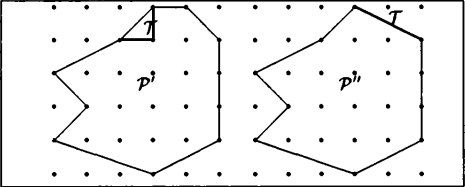
\includegraphics[height=20mm]{kartina1}
\end{wrapfigure}
как эти параллелограммы не имеют ни одной 
внутренней точки в $\mathbb {Z}^{2}$, то объединение их вершин 
является в точности квадратной сеткой $\mathbb {Z}^{2}$, и, 
следовательно, $\{\vec{u},\vec{v}\}$ образуют систему образующих $\mathbb {Z}^{2}$. 
Отсюда следует, что $\{\vec{u},\vec{v}\}$ является базисом $\mathbb {Z}^{2}$ и $|det(\vec{u},\vec{v})| = 1$ является числом, представляющим площадь параллелограмма (площадь треугольника равна половине площади параллелограмма), что совпадает с формулой Пика.

\subparagraph{b.} Рассмотрим два приведения $\mathcal{P} \rightarrow \mathcal{P}'$ и $\mathcal{P} \rightarrow \mathcal{P}''$. Первое состоит в присоединении внутренней точки $\mathcal{P}$ к двум вершинам. Второе --- в присоединении двух вершин $\mathcal{P}$ так, чтобы треугольник $\mathcal{T}$, ограниченный таким образом, отвечал условиям пункта {\bf a} (см. рис. 1).

В первом случае получают многоугольник $\mathcal{P}'$ с характеристикой $(n',f')$, а во втором случае — многоугольник $\mathcal{P}''$ с характеристикой $(n'',f'')$, связанные отношениями:
\begin{equation*}
i' = i - 1,\qquad f' = f + 1,\qquad i'' = i,\qquad f'' = f - 1,
\end{equation*}

\begin{tabular}{ccl} 
площадь($\mathcal{T}$) = $\frac{1}{2}$,$\;\;$ площадь($\mathcal{P}$) &=& площадь($\mathcal{P}'$) + площадь($\mathcal{T}$) = \\
                                                       &=& площадь($\mathcal{P}''$) + площадь($\mathcal{T}$).
\end{tabular} 

\begin{figure}[h]
\center{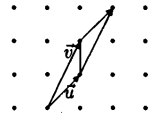
\includegraphics[width=90mm]{kartina2}}
\caption{Приведения многоугольника}
\end{figure}



\noindent Эти соотношения доказывают, что если формула Пика истинна для $\mathcal{P}'$ (соответственно для $\mathcal{P}''$), она истинна и для $\mathcal{P}$. Здесь был использован тот факт, что можно всегда применить одно из двух приведений, что позволяет доказать формулу Пика по индукции.

\subsection{\normalsize{29. Теорема о ядре}}

\subparagraph{а.} Пусть $b_{i} = a_{1}a_{2}\ldots a_{i-1}a_{i+1}\ldots a_{k}$. Тогда $b_{i}$ взаимно просты, следовательно, существуют такие $u_{1},\ldots,u_{k}$, что 1 = $u_{1}b_{1}+u_{2}b_{2}+\dots+u_{k}b_{k}$. Для $x \in M$ имеет место равенство:
\begin{equation}
x = u_{1}b_{1}x + u_{2}b_{2}x +\dots+ u_{k}b_{k}x,\;\;\;\text{и}\;\;\;x \in Ker_{M} a_{2} \Rightarrow b_{i}x \in Ker_{M} a_{i},
\end{equation}

\noindent откуда следует равенство $Ker_{M} a = Ker_{M} a_{1} + Ker_{M} a_{2} +\dots+ Ker_{M} a_{k}$.

С другой стороны, если $x_{i} \in Ker_{M} a_{i}$, то $u_{j}b_{j}x_{i} = 0$ для $j \neq i$. В силу свойства (8): $x_{i} = u_{i}b_{i}x_{i}$. Следовательно, соотношение $\sum_{i = 0}^{k}x_{i} = 0$ влечет $x_{j} = 0$ и то, что сумма прямая.



%\lhead{404}
%\rhead{\rm{III} \small\textit{Модули над кольцами главных идеалов}}

\subparagraph{с.} Имеют место равенства:
\begin{equation*}
(X - \lambda) \bullet e^{\lambda t}f = e^{\lambda t}\frac{df}{dt},\;\;\;\;\; (X - \lambda)^{n} \bullet e^{\lambda t}f = e^{\lambda t}\frac{d^{n}f}{dt^{n}},
\end{equation*}

\noindent и следовательно, ${\rm Ker}(X - \lambda)^{n} = \{R(t)e^{\lambda t} \;|\; R(t) \in \mathbb {C}[t],\;\;{\rm deg}(R) < n\}$.

\subsection{\normalsize{31. Примарные модули над кольцом главных идеалов (задача)}}

\subparagraph{a.} Из равенства $M = N \pi M$ следует:
\begin{equation*}
M = N + \pi N + \pi^{2}M = N + \pi^{2}M =\dots= N + \pi^{3}M=\dots= N + \pi^{k}M = N,
\end{equation*}

\noindent что доказывает пункт ($i$).

\par (\textit{$ii$}) $M = \sum_{i \in I}Ax_{i}\;+\;\pi M$, тогда в силу предыдущего результата\linebreak
$M = \sum_{i \in I}Ax_{i}$, минимальность доказывается легко.

\par (\textit{$iii$}) Если $\pi$ не делит $\alpha$, то $\pi^{k}$ и $\alpha$ взаимно просты, тогда 1 является
линейной комбинацией $\alpha$ и $\pi^{k}$, а так как $x$ обнуляется сразу значениями
$\pi^{k}$ и $\alpha$, то $x = 0$. Получили противоречие.

\par (\textit{$iv$}) Заметим, что $\sum_{i}\mu_{i}x_{i} = 0 \Rightarrow \pi \;|\; \mu_{i}$. Действительно, используя
то, что сумма $\sum_{i \in I}A\pi x_{i}$ прямая, имеем: вышеприведенное равенство,
умноженное на $\pi$, дает $\mu_{i}\pi x_{i} = 0$. Так как $\pi x_{i} \neq 0$, то, в силу предыдущего результата, $\pi | \mu_{i}$.

В $M/\pi M$ равенство вида $\sum_{i \in I}\overline{\lambda_{i}}\overline{x}_{i} = 0$, влечет равенства\linebreak
$\sum_{i \in I}\lambda_{i}x_{i} = \pi\sum_{i \in I}\beta_{i}x_{i}$ и $\sum_{i \in I}(\lambda_{i} - \pi\beta_{i}) = 0$. В силу предыдущего
результата $\pi |\lambda_{i} - \pi\beta_{i} \Rightarrow \pi \;|\; \lambda_{i} \Rightarrow \overline{\lambda_{i}} = 0$, что и надо было доказать.

\subparagraph{b.} Запишем $\pi M$ в виде прямой суммы ненулевых однопорожденных
подмодулей:
\begin{equation}
\pi M = \bigoplus_{i \in I} A\pi x_{i},\;\;\; \text{ где }\;\;\; \pi x_{i} \neq 0.
\end{equation}

\noindent Тогда из пункта $(iv)$ вопроса {\bf a} известно, что множество $(\overline{x}_{i})_{i \in I}$ является линейно независимым множеством векторного $A/\pi A$-пространства
$M/\pi M$. Дополним это множество до базиса $M/\pi M$. Пусть\linebreak
$(\overline{x}_{i})_{i \in I} \cup (\overline{z}_{j})_{j \in J}$ --- это базис.

Равенство (9) доказывает, что $\pi z_{j} \in \bigoplus_{i \in I}A\pi x_{i}$, т.е.
$\pi z_{j} = \sum_{i \in I}a_{ij}\pi x_{i}$. Положим $u_{j} = z_{j} - \sum_{i \in I}a_{ij}x_{i}$; множество
$(\overline{x}_{i})_{i \in I} \cup (\overline{z}_{j})_{j \in J}$ будет всегда базисом $M/\pi M$, и в этом случае $u_{j}$ обнуляется $\pi: \pi u_{j} = 0$.

Докажем, что $M$ является прямой суммой следующих однопорожденных модулей:
\begin{equation*}
M = \bigoplus_{i \in I} Ax_{i} \oplus \bigoplus_{j \in J} Au_{j}.
\end{equation*}



%\lhead{\small\textit{Решение упражнений}}
%\rhead{405}

\noindent Прежде всего, это множество является системой образующих, как это
было доказано во втором пункте $(ii)$ предыдущей задачи. Рассмотрим
соотношение $\sum_{i \in I}a_{i}x_{i} + \sum_{j \in J}b_{j}u_{j} = 0$. Приводя по модулю $\pi M$, получим $\pi\;|\;a_{i}$ и $\pi\;|\;b_{j}$. Из соотношения $\pi u_{j} = 0$ следует, что $b_{j}u_{j} = 0$. Если
записать $a_{i}$ в виде $a_{i} = \pi c_{i}$, получим $\sum_{i \in I} c_{i}\pi x_{i}$, а так как сумма
в (9) прямая, то $c_{i}\pi x_{i} = a_{i}x_{i} = 0$, что и требовалось доказать.

\subparagraph{с.} Достаточно рассмотреть последовательность
\begin{equation*}
0 = \pi^{k}M \subset \pi^{k-1}M \subset\dots\subset \pi M \subset M
\end{equation*}

\noindent и заметить, что теорема истинна для подмодуля $\pi^{k-1}M$, который является векторным $A/\pi A$-пространством. Простая индукция по $k$ доказывает теорему.

\subsection{\normalsize{32. Абелевы группы данного порядка $n$}}

\subparagraph{а.} Пусть дана абелева группа $\Omega$ порядка $p^{r}$. Существует возрастающая последовательность $(r_{1},r_{2},\ldots,r_{s})$ целых строго положительных
чисел, удовлетворяющих условию $r_{1} + r_{2} +\dots+ r_{s} = r$, и такая, что
$\Omega$ будет изоморфна $\mathbb {Z}_{p^{r_{1}}} \times \mathbb {Z}_{p^{r_{2}}} \times \dots \times \mathbb {Z}_{p^{r_{s}}}$, и эта последовательность
определяется единственным образом по структуре $\Omega$. Итак, достаточно пронумеровать все такие последовательности (которые не зависят
от $p$). Для этого зафиксируем длину $s,\; 1 \leqslant s \leqslant r$, и рассмотрим лексикографический порядок на возрастающих последовательностях целых
положительных чисел длины $s$ суммы $r$. Наименьшая последовательность будет $(1,1,\ldots,1,r - (s - 1))$. «Хорошей» последовательностью в
лексикографическом порядке $(r_{1},r_{2},\ldots,r_{s})$ будет последовательность
$(r'_{1},r'_{2},\ldots,r'_{s})$, постоянная на местах $[i,s - 1]$ для определенного $i$:
\begin{gather}
(r_{1},r_{2},\ldots,r_{i-1},1 + r_{i},\ldots,1 + r_{i},r'_{s}), \nonumber \\
\text{где}\;\;r_{1} +\dots+ r_{i-1} + (s-i)(1 + r_{i}) + r'_{s} = r.
\end{gather}

\noindent Из соотношения (10) следует:
\begin{gather*}
r'_{s} = r - (r_{1} + r_{2} +\dots+ r_{i-1}) - (s-i)(1 + r_{i}) = \\
       = (r_{i} + r_{i+1} +\dots+ r_{s}) - (s-i)(1 + r_{i}).
\end{gather*}

\noindent Чтобы сохранить возрастание, достаточно наложить условие $1 + r_{i} \leqslant r'_{s}$,
т.е.:
\begin{equation}
(s - i + 1)(1 + r_{i}) \leqslant (r_{i} +\dots+ r_{s})
\end{equation}

\noindent  Итак, «хорошей» будет последовательность (10), а индекс $i$ будет наибольшим, удовлетворяющим условию (11). Это дает алгоритм 8.


    %\rhead{\emph{\leftmark}}
    %\lhead{\thepage}

    %%%%%%%%%%%%%%%%%%%%%%%%%%%%%%%%%%%%%%%%%%%%%%%%%%%%%%%%%%%%%%%%%%%%%%%\
    % это можно убрать при сшивке с предыдущими страницами

    \setcounter{chapter}{3}
    % ОБЯЗАТЕЛЬНО ДВА РАЗА
    %\chapter[Модули над кольцами главных идеалов]{Модули над кольцами главных идеалов}
    %\thispagestyle{empty} % обязательно после chapter!!!

    %\setcounter{section}{10}
    %\section{Решения упражнений}

    \setcounter{subsection}{32}
    %\subsection{Абелевы группы данного порядка $n$}

    %%%%%%%%%%%%%%%%%%%%%%%%%%%%%%%%%%%%%%%%%%%%%%%%%%%%%%%%%%%%%%%%%%%%%%%

    \chaptertop
    \setcounter{page}{406}
    %\restoretop

    \setcounter{lstlisting}{7}
    \begin{center}
    \begin{minipage}{0.80\textwidth}
    \begin{lstlisting}[
    mathescape=true,
    captionpos={bo},
    caption={Коррекция последовательности $(r_1, \ldots, r_s)$}\label{euclid}
    ]
    	$u \gets 0$;
    	for $i$ $\textbf{in}$ $s...1$ do
    		$u \gets u + r_i;\quad▷\ u = r_i + ... + r_s;$
    		if $(s − i + 1)(1 + r_i ) \leqslant u$ then
    			$r_s \gets u − (s − i)(1 + r_i);$
    			$r_i...s−1 \gets 1 + r_i$;
    			exit;
    		end if
    	end for
    \end{lstlisting}
    \end{minipage}
    \end{center}

    %\setcounter{algorithm}{7}
    %\begin{algorithm}
    %\caption{Коррекция последовательности $(r_1, \ldots, r_s)$}\label{euclid}
    %\begin{algorithmic}
    %\State $u\gets 0;$
    %\For{$i$ \textbf{in} $s...1$}
    %\State $u\gets u + r_i;$ \Comment{$u = r_i + ... + r_s;$}
    % \If{$(s-i+1)(1+r_i) \leqslant u$}
    % \State $r_s \gets u - (s - i)(1 + r_i);$
    % \State $r_{i\ldots s-1} \gets 1 + r_i;$
    % \State \textbf{exit;}
    % \EndIf;
    %\EndFor;
    %\end{algorithmic}
    %\end{algorithm}

    Например, для $r = 6$ получаем следующие $\rho(6) = 11$ последователь-\linebreak ностей:
    \begin{gather*}
    (6),\quad (1, 5),\quad (2, 4),\quad (3, 3),\quad (1, 1, 4),\quad (1, 2, 3),\quad (2, 2, 2),\\
    (1, 1, 1, 3), \quad (1, 1, 2, 2), \quad (1, 1, 1, 1, 2),\quad (1, 1, 1, 1, 1, 1),
    \end{gather*}
    которые образуют для $p = 2$ одиннадцать абелевых групп порядка 64:
    \begin{gather*}
    \mathbb{Z}_{64},\quad \mathbb{Z}_2\times \mathbb{Z}_{32},\quad \mathbb{Z}_4\times \mathbb{Z}_{16},\quad \mathbb{Z}_8 \times \mathbb{Z}_8,\quad \mathbb{Z}_2 \times \mathbb{Z}_2 \times \mathbb{Z}_{16},
    \quad \mathbb{Z}_2\times \mathbb{Z}_4 \times \mathbb{Z}_8 ,\\ \quad \mathbb{Z}_4 \times \mathbb{Z}_4 \times \mathbb{Z}_4,\quad \mathbb{Z}_2 \times \mathbb{Z}_2 \times \mathbb{Z}_2 \times \mathbb{Z}_8 ,\quad \mathbb{Z}_2 \times \mathbb{Z}_2\times \mathbb{Z}_4 \times \mathbb{Z}_4 ,\\ \quad \mathbb{Z}_2 \times \mathbb{Z}_2 \times \mathbb{Z}_2 \times \mathbb{Z}_2\times \mathbb{Z}_4,\quad \mathbb{Z}_2 \times \mathbb{Z}_2 \times \mathbb{Z}_2 \times \mathbb{Z}_2 \times \mathbb{Z}_2 \times \mathbb{Z}_2.
    \end{gather*}

    Приведем таблицу чисел $\rho(r)$\footnote{Заметим, что число $\rho(r)$ равно $\rho(r)$, числу разбиений $r$ на меньшие слагаемые, так что для определения значения $\rho(r)$ при больших $r$ можно воспользоваться знаменитой формулой Рамануджана, дающей решению задачи partitio numerorum.~— {\slshape Прим. перев.}}:

    \begin{table}[h!]
    \centering
    \label{my-label}
    \begin{tabular}{|l|cccccccccc|}
    \hline
    \multicolumn{11}{|c|}{\begin{tabular}[c]{@{}c@{}}$\rho_r = $ число абелевых групп порядка $\rho^r$,\\ $\rho$~— произвольное простое число\end{tabular}} \\ \hline
    $r$ & 1 & 2 & 3 & 4 & 5 & 6 & 7 & 8 & 9 & 10 \\
    $\rho_r$ & 1 & 2 & 3 & 5 & 7 & 11 & 15 & 22 & 30 & 42 \\ \hline
    $r$ & 11 & 12 & 13 & 14 & 15 & 16 & 17 & 18 & 19 & 20 \\
    $\rho_r$ & 56 & 77 & 101 & 135 & 176 & 231 & 297 & 385 & 490 & 627 \\ \hline
    \end{tabular}
    \end{table}

    {\bfseries b.\;}\,Отношение Безу $1 = u\,n + v\,m\,$ для $\,x \in \Omega\,$ влечет $\,x = v\,m\,x + u\,n\,x$ и $\,\Omega = \Omega^{(n)} \oplus \Omega^{(m)}\,$. Остается определить порядок $\Omega^{(n)}$. Так как $\Omega^{(n)}$~— конечная абелева группа, обнуляющаяся $n$, то она является
    частным от степени $\mathbb{Z}_n$ и, следовательно, если простое $p$ делит порядок группы $\Omega^{(n)}$, то $p$ делит $n$. Разложение на простые множители порядка группы $\Omega^{(n)}$ (соответственно группы $\Omega^{(m)}$) состоит из простых делителей $n$ (соответственно $m$). А так как $\card \Omega^{(n)} \times \card \Omega^{(m)} = n\,m$, то $\card \Omega^{(n)} = n$ и $\card \Omega^{(m)} = m$.

    {\bfseries c.\;}\,Если $\Omega^\prime\,$ и $\,\Omega^{\prime\prime}$~— две абелевы группы порядков, соответственно, $n$ и $m$, то $\Omega^\prime \times \Omega^{\prime\prime}$~— абелева группа порядка $n\,m$. Обратно, группа $\Omega$ порядка $n\,m$, где $n$ и $m$ взаимно просты, представляется единственным образом в виде произведения группы порядка $n$ и группы порядка $m$. Действительно, $\Omega = \Omega^{(n)} \oplus \Omega^{(m)}$ и, кроме того, если $\Omega = \Omega^\prime \oplus \Omega^{\prime\prime}$, где $|\Omega^\prime| = n$ и $|\Omega^{\prime\prime}| = m$, то $\Omega^\prime = \Omega^{(n)}$ и $\Omega^{\prime\prime} = \Omega^{(m)}$. Таким образом, получили, что любые абелевы группы порядка $nm$ представляются в виде произведения абелевой группы порядка $n$ и абелевой группы порядка $m$ (и к тому же единственным способом), откуда следует мультипликативность $\theta$.

    Если $p^{r_1}_1p^{r_2}_2 \ldots p^{r_k}_k$~— разложение на простые множители числа $n$, то \linebreak $\theta(n)=p(r_1)p(r_2) \ldots p(r_k)$, и имеются $42$ абелевы группы порядка $21\,600$.

    \subsection{\normalsize {Вычисление инвариантных множителей}}

    {\bfseries a.\;}\,Если положить $ f_1 = e_1 + \ldots + e_n,\,f_2 = e_1 - e_2,\,f_3 = e_1 - e_3, \ldots ,\,f_n = e_1 - e_n$, то $\{f_1, e_2, e_3, \ldots, e_n\}$ будет базисом $\mathbb{Z}^n$, а его первый вектор будет базисом $F$, в то время, как множество $\{e_1, f_2, f_3, \ldots, f_n\}$ будет базисом $\mathbb{Z}^n$, а его последние $n-1$ векторов будут образовывать базис $E$.

    {\bfseries b.\;}\,$\{f_1, f_2, \ldots, f_n\}$~— базис $E \oplus F$, его матрицей в каноническом базисе будет первая из приведенных ниже матриц. Если в этой матрице прибавить к столбцу 1 столбец 2, столбец 3, \ldots, затем столбец $n$, то получим матрицу, вторую по порядку. Теперь достаточно прибавить к строке 1 строку 2, строку 3, \ldots, затем строку $n$, и мы получим матрицу, изображенную последней.

    \[ \begin{pmatrix}
    1 & 1 & 1 && 1\\
    1 & -1 & 0 && 0\\
    1 & 0 & -1 && 0\\
    \vdots & \vdots & \vdots && \vdots\\
    1 & 0 & 0 && -1
    \end{pmatrix},\quad
    \begin{pmatrix}
    n & 1 & 1 && 1\\
    0 & -1 & 0 && 0\\
    0 & 0 & -1 && 0\\
    \vdots & \vdots & \vdots && \vdots\\
    0 & 0 & 0 && -1
    \end{pmatrix},
    \]

    \[ \begin{pmatrix}
    n & 0 & 0 && 0\\
    0 & -1 & 0 && 0\\
    0 & 0 & -1 && 0\\
    \vdots & \vdots & \vdots && \vdots\\
    0 & 0 & 0 & \dots & -1
    \end{pmatrix}
    .\]

    \newpage

    \subsection{\normalsize{Другое вычисление инвариантных множителей}}

    Метод приведения дает следующие матрицы:

    \[ L = \begin{pmatrix}
    1 & 0 & 0 & 0\\
    2 & 1 & 0 & 0\\
    -1 & -1 & 1 & 0\\
    -1 & -6 & 0 & 1
    \end{pmatrix},\quad
    R = \begin{pmatrix}
    -3 & 10 & -2\\
    2 & -7 & -1\\
    0 & 0 & 1\\
    \end{pmatrix},
    \]

    \[ X^\prime = \begin{pmatrix}
    -1 & 0 & 0\\
    0 & -6 & 0\\
    0 & 0 & 0\\
    0 & 0 & 0
    \end{pmatrix},
    \] при этом $X^\prime = LXR$, $L$ и $R$ имеют определители 1. Матрица $L$ индуцирует изоморфизм из $\mathbb{Z}^4/\im{X}$ в $\mathbb{Z}^4/\im{X}^\prime$, который выражается равенствами:
    $$ L(f_1) = \overline{e}_1 + 2\overline{e}_2-\overline{e}_3-\overline{e}_4,\quad L(f_2) = \overline{e}_2-\overline{e}_3-6\overline{e}_4,\quad L(f_3) = \overline{e}_3,\quad L(f_4) = \overline{e}_4,$$
    и дает, обращая формулы, приведенные выше, следующие искомые образующие $M$: $g_1 = f_1 - 2f_2 - f_3 - 11f_4 = 0,\,g_2 = f_2 + f_3 + 6f_4,\,g_3 = f_3$, и $\,g_4 = f_4$.

    \subsection{\normalsize{Инвариантные множители и НОД миноров}}

    Пусть $b_i$~— наибольший общий делитель миноров $X$ порядка $i$ для \linebreak $i = 1,\,2,\,3$.
    Число 2 делит все коэффициенты $X$, и существует пара коэффициентов, имеющая 2 своим наибольшим общим делителем (например, 6 и 10); следовательно, $b_1 = 2$. С другой стороны, 4 делит все миноры порядка 2 (если 2 делит $a, b, c, d,$ то 4 делит $ad - bc$), и существуют два минора порядка 2, имеющие 4 своим наибольшим общим делителем, например:

    $$\begin{vmatrix}
    8 & 4\\
    4 & 4
    \end{vmatrix} = 16 = 2^3 \quad\mathrm{и}\quad \begin{vmatrix}
    18 & 30\\
    4 & 10
    \end{vmatrix} = 60 = 2^2 \times 3 \times 5, $$
    что влечет $b_2 = 4$. Приведем миноры порядка 3:
    \begin{align*}
    \begin{vmatrix}
    8 & 4 & 20\\
    12 & 18 & 30\\
    4 & 4 & 10
    \end{vmatrix} = 0,\quad \begin{vmatrix}
    6 & 4 & 20\\
    12 & 18 & 30\\
    18 & 4 & 10
    \end{vmatrix} &= -3\,480,\\
    \begin{vmatrix}
    6 & 8 & 20\\
    12 & 12 & 30\\
    18 & 4 & 10
    \end{vmatrix} = 0,\quad \begin{vmatrix}
    6 & 8 & 4\\
    12 & 12 & 18\\
    18 & 4 & 4
    \end{vmatrix} &= 1\,392.
    \end{align*}
    \newpage
    Это дает $b_3 = \Nod(1\,392, 3\,480) = 696$. Следовательно, инвариантные \linebreak множители $a_1, a_2, a_3$ задаются равенствами: $a_1 = b_1 = 2,\, a_1a_2 = b_2 = 4,$\,\linebreak $a_1a_2a_3 = b_3 = 696$, откуда $a_1 = 2,\,a_2 = 2\,$ и $\,a_3 = 174$, что совпадает с результатами в данной главе!
    \subsection{\normalsize{Условие наличия одинаковых инвариантных множителей\\ относительно $A^n$}}

    Если $E$ и $F$ имеют одни и те же инвариантные множители, ясно, что $A^n/E$ и $A^n/F$ изоморфны. Обратно, предположим, что $A^n/E$ и $A^n/F$ изоморфны, и пусть $E^\prime \subset A^n$ (соответственно $F^\prime \subset A^n$) ~— нормальный подмодуль, эквивалентный $E$ (соответственно $F$):
    $$E^\prime = a_1A \times a_2A \times \ldots \times a_nA,\quad F^\prime = b_1A \times b_2A \times \ldots \times b_nA,$$
    где $a_i\,|\,a_{i+1}\,$ и $\,b_i\,|\,b_{i+1}$. Модули частные $A^n/E^\prime$ и $A^n/F^\prime$ тогда изоморфны (так как первый изоморфен $A^n/E$, а второй изоморфен $A^n/F$). Пусть $p$ и $q$ индексы, удовлетворяющие условию:
    $$i \in [1, p] \Leftrightarrow a_i \in U(A)\quad\mathrm{и}\quad j \in [1, q] \Leftrightarrow b_j \in U(A).$$
    Тогда $n-p = n-q$, и для $p < i \leqslant n\quad a_iA = b_iA$. Следовательно, $a_iA = b_iA$ для всех $i \in [1, n]$, что влечет равенство $E^\prime = F^\prime$. Итак, подмодули $E$ и $F$ эквивалентны в $A^n$: $E$ и $F$ имеют одни и те же инвариантные множители.



    \subsection{\normalsize{Определяющие соотношения}}

    Пусть $(e_1, e_2, e_3)$~— канонический базис $\mathbb{Z}^3$, a $\varphi -$ {\bf{сюръективный}} морфизм из $\mathbb{Z}^3$ на $\Omega$, который преобразует $e_i$ в $g_i$. Если $X$~— транспонированная матрица системы, то $\im X \subset \Ker\varphi$ и имеет место сюръекция из $\mathbb{Z}^3/\im X$ на $\mathbb{Z}^3/\Ker\varphi \simeq \Omega$. Следовательно, $\Omega$ изоморфна фактор-группе $\mathbb{Z}^3/\im X$. Но $\mathbb{Z}^3/\im X$ является группой с $|\det(X)| = 19$ элементами \ldots

    Можно вычислить две матрицы $L$ и $R$ c определителем 1 и такие, что матрица $X^\prime = LXR$ будет приведенной, например:
    $$ L = \begin{pmatrix}
    1 & 0 & 0\\
    0 & -1 & 0\\
    -2 & 5 & 1
    \end{pmatrix},\quad X^\prime = \begin{pmatrix}
    1 & 0 & 0\\
    0 & -1 & 0\\
    0 & 0 & 19
    \end{pmatrix},$$
    $$R = \begin{pmatrix}
    -8 & -25 & -132\\
    1 & 3 & 14\\
    0 & 0 & 1
    \end{pmatrix}.$$

    \newpage
    \noindent Тогда в $\mathbb{Z}^3/ImX^\prime \simeq \mathbb{Z}/19\mathbb{Z}$\quad\quad$g_1 = \overline{L(e_1)},\,\,g_2 = \overline{L(e_2)},\,\,g_3 = \overline{L(e_3)}$ будет образовывать такую систему. В данном примере $g_1 = -2,\,g_2 = 5\,$ и $\,g_3 = 1$.
    \subsection{\normalsize{Образующие и определяющие соотношения (продолжение)}}

    Пусть $(e_1, e_2, e_3)$~— канонический базис $\mathbb{Z}^3$, а $\varphi$~— {\bf{сюръективный}} морфизм из $\mathbb{Z}^3$ на $\Omega$, который переводит $e_i$ в $g_i$. Если $X$~— транспонированная матрица системы, то $\im X \subset \Ker
    \varphi$ и имеет место сюръекция из $\mathbb{Z}^3/\im X$ на $\mathbb{Z}^3/\Ker \varphi \simeq \Omega$. Следовательно, $\Omega$ изоморфна факторгруппе $\mathbb{Z}^3/\im X$. Но $\mathbb{Z}^3/\im X$ является группой с $|\det X| = 288$ элементами. Действительно, приведение инвариантных множителей показывает, что $X$ эквивалентна приведенной матрице $X^\prime$:

    $$ X = \begin{pmatrix}
    2 & 8 & 72\\
    4 & 20 & 72\\
    -6 & -16 & 324
    \end{pmatrix},\quad X^\prime = \begin{pmatrix}
    2 & 0 & 0\\
    0 & 4 & 0\\
    0 & 0 & 36
    \end{pmatrix},$$
    и, следовательно:
    $$\mathbb{Z}^3/\im X \simeq \mathbb{Z}^3/\im X^\prime \simeq \mathbb{Z}_2 \times \mathbb{Z}_4 \times \mathbb{Z}_{36} = \Omega^\prime.$$
    Если $\overline\varphi$ обозначает сюръекцию из $\Omega^\prime$ на $\Omega$, то подгруппа $96\Omega^\prime$ из $\Omega^\prime$ содержится в $\Ker\overline\varphi$ ($\Omega$ будет группой порядка 96, тогда $96\Omega = \{0\}$). Эта подгруппа имеет индекс 96 (или порядок 3), и, следовательно, $\overline\varphi$ индуцирует сюръекцию из $\Omega^\prime/96\Omega^\prime$ на $\Omega$, которая будет изоморфизмом (эти две группы имеют идентичные порядки). Остальное следует из того, что $\mathbb{Z}_{36}/96\mathbb{Z}_{36}\simeq \mathbb{Z}_{12}$.
    \subsection{\normalsize{Упражнение Чарльза Лутвиджа Доджсона}}
    %\textsf
    { \ldots Place 8 pigs in the first sty, 10 in the second, nothing in the third, and 6 in the fourth: 10 is nearer ten than 8; nothing is nearer ten than 10; 6 is nearer ten than nothing; and 8 is nearer ten than~6\footnote{B первом свинарнике должно находиться 8 поросят, во втором — 10 и в четвертом 6. Ничего не должно находиться в третьем свинарнике: он должен быть пуст... Десять ближе к 10, чем 8. Что может быть ближе к 10, чем~10? Ничто! Но именно «ничто» и находится в третьем свинарнике. Шесть ближе к~10, чем~О (арифметический псевдоним «ничего»), 8 ближе к~10, чем~6...
    \begin{flushright} (Перевод Ю. А. Данилова, Л. Кэррол «История с узелками», М., Мир, 1973.)\end{flushright}}.

    \begin{flushright} (Lewis Carroll, \textit {A tangled tale} (1885 [44])\end{flushright}}
    %~\cite{Carrol1982}

    \setcounter{section}{0}

    \chapter[Некоторые методы алгебраической алгоритмики]{Некоторые методы \\ алгебраической \\ алгоритмики}
    \thispagestyle{empty}

    \epigraph {Although unique factorization for integers is sometimes called the
    “fundamental theorem of arithmetic,” it is only occasionally that a
    student learns anything about the constructive aspects of this
    thm beyond the most elementary facts. Yet there are interesting
    unsolved mathematical and computational problems involved in
    factorization of integers and tests of primality and many of the ideas
    involved are accessible to undergraduate students\footnotemark[1].}{John D. Dixon, \emph{ Factorization and primality tests} (1984 [67])}
    %~\cite{Dixon1974}
    \footnotetext[1]{Хотя единственность разложения целых чисел на простые множители иногда называют «основной теоремой арифметики», студенты редко изучают конструктивные аспекты этой теоремы, кроме, быть может, самых элементарных фактов. Все еще существуют интересные нерешенные математические и комбинаторные проблемы, связанные с разложением целых чисел на множители с проверкой простоты, и многие из используемых там идей доступны студентам.}
    К этому моменту нами получены почти все предварительные результаты за исключением быстрого преобразования Фурье, которое будет детально изучено в главе V, и мы можем начать исследование в области алгоритмической алгебры или, по крайней мере, в той ее
    части, где добились наибольшего успеха, — в области чисел. Как следует из дальнейшего изложения, многие используемые алгоритмы
    опираются на четыре основных метода: алгоритм экспоненциальной дихотомии, алгоритм Евклида, китайскую теорему об остатках (которую мы
    изучим в этой главе) и быстрое преобразование Фурье, которое позволяет, используя алгоритм Полларда, эффективно перемножать большие числа. Конечно,
    этот подход, основанный на редукции, не слишком богат \textit{абстрактными} теоретическими результатами.\\
    \indent Как и Диксон, мы убеждены, что некоторые формальные результаты доступны даже новичку, хотя бы потому, что часто можно привести конкретную и простую иллюстрацию этих результатов. Китайская теорема об остатках, например, записанная формально, действительно может показаться абстрактной (какой-то непонятный идеал в каком-то кольце\ldots); и можно верить в ее так называемую эффективную форму до того момента, когда действительно придется использовать ее для {\textbf{вычислений}}.\linebreak Тогда переходят к менее «возвышенному» этапу, заключающемуся в изучении всех необходимых вычислений, для того, чтобы уловить все нюансы и учесть их при реализации\ldots\;В конце концов приходят, таким образом, к лучшему пониманию богатства чисел. Изучение группы обратимых по модулю $n$ элементов кажется иногда чисто алгебраическим упражнением; несколько конкретных примеров показывают, что эта группа так или иначе определяет структуру числа $n$: если имеются только два квадратных корня из 1 по модулю $n$, то $n$ — степень простого числа\ldots\;Можно указать конкретный вид этой группы, найти ее образующие, установить, что, насколько структура $\mathbb{Z}/n\mathbb{Z}$ регулярна и понятна, настолько структура группы обратимых элементов, спроектированная, как это обычно делается, на интервал $[1, n — 1]$, хаотична и сбивает с толку.\\
    \indent В противоположность некоторым понятиям, которые новичку кажутся сложными, ~— например, квадратичные вычеты, кажущаяся сложность которых обязана большей частью тому названию, которое наши предки дали квадрату (однако, слово \textit{собака} не кусается) ~— существуют очень простые понятия, доступные любому студенту, например, делители нуля в некотором кольце. Но сколько же пользы извлекли из этих особых элементов, которых старались избегать! Например, делитель нуля по модулю $n$ немедленно приводит к разложимости $n$ (благодаря, скажем, алгоритму Евклида); это является основой классических методов проверки чисел на простоту (Rabin-Miller) или вычисления квадратных корней по модулю $n\ldots$\\
    \indent В этой главе мы надеемся показать, что все эти понятия имеют простую интерпретацию, возможно, основанную на редукции, но
    позволяющую, по крайней мере, уменьшить страхи, которые мы испытываем при приближении к загадочному миру чисел.

    \epigraph {Итак, чтобы понять теорию, недостаточно констатировать, что выбранная дорога свободна от препятствий, нужно отдавать себе отчет что заставило выбрать ее. Сможем ли мы когда-нибудь сказать, что понимаем теорию, если хотим придать ей сразу окончательную форму, которую навязывает ей безукоризненная логика, чтобы не осталось никакого следа от действий наугад, которые к ней привели? Нет, в действительности мы не сможем ее понять, не сможем даже запомнить и не запомним, даже выучив наизусть.}{А. Пуанкаре, \textit{Сочинения} (1899 [161]) }
    %\cite{Schmid1978}

    \section{Кольцо $\mathbb{Z}/n\mathbb{Z}$}

    \noindent В начале этой главы мы напомним несколько основных свойств кольца $\mathbb{Z}/n\mathbb{Z}$, затем установим связь с элементарной реализацией необходимых операций для вычислений в этом кольце.

    Как принято в такого рода исследованиях, в тех случаях, когда исключена неопределенность, мы будем одинаково обозначать элемент
    кольца $\mathbb{Z}$ и его класс по модулю $n$. Если необходимо, то класс $x$ по модулю $n$ будем обозначать через $\overline{x}$ или $x \bmod n$.

    \begin{predl}
    \hspace*{0.5cm}
    Пусть $b$~— целое, а $n$~— положительное целое число. Следующие утверждения эквивалентны:

    {\bfseries a.\;} $b$ обратимо по модулю $n$,

    {\bfseries b.\;} $b$~— образующий аддитивной группы $\mathbb{Z}/n\mathbb{Z}$,

    {\bfseries c.\;} $n$ и $b$ взаимно простые.

    \end{predl}

    \begin{myproof}
    ${\bf {a \Rightarrow b}}$. Пусть $p$~— порядок $b$, тогда $pb \equiv 0\,\,(\!\!\!\mod{n})$, откуда, в силу обратимости $b, p \equiv 0\,\,(\!\!\!\mod{n})$.
    Значит, порядок $b$ делится на $n$ и, следовательно, равен $n$.\\\\
    ${\bf {b \Rightarrow c}}$. Так как $b$~— образующий, то существует $x$ такой, что $bx \equiv 1\linebreak(\!\!\!\mod{n})$, откуда $bx + kn = 1$~— равенство, являющееся соотношением Безу для $b$ и $n$.\\

    \noindent${\bf{c \Rightarrow a}}$. Запишем соотношение Безу между $b$ и $n$: $u b + v n = 1$ и рассмотрим его по модулю $n$. Коэффициент Безу $u$ и есть обратный к $b$.
    \end{myproof}
    \newpage
    Можно упростить алгоритм вычисления коэффициентов Безу и применить его для определения обратных к элементам из $\mathbb{Z}/n\mathbb{Z}$. Действительно, для этих вычислений не нужно выражать в явном виде коэффициент\linebreak Безу при $n$ и, следовательно, из алгоритма, данного во второй главе, можно исключить несколько ненужных переменных (см. алгоритм 1).

    \setcounter{lstlisting}{0}
    \begin{center}
    \begin{minipage}{0.85\textwidth}
    \begin{lstlisting}[
    mathescape=true,
    captionpos={bo},
    caption={Обращение $b$ в $\mathbb{Z}/n\mathbb{Z}$}
    ]
 $\begin{pmatrix}
    u\\
    u^{\prime}
    \end{pmatrix} \gets \begin{pmatrix}
    1\\
    0
    \end{pmatrix}; \quad \begin{pmatrix}
    r\\
    r^{\prime}
    \end{pmatrix} \gets \begin{pmatrix}
    b\\
    n
 \end{pmatrix};$
 while $r^{\prime} \ne 0$ do
    $▷\;\Nod(r, r^{\prime}) = \Nod(b, n),\ u\,b \equiv r\,\pmod{n}\;\mathrm{и}\;u^{\prime}\,b \equiv r^{\prime}\pmod{n}.$

    $q \gets r / r^{\prime};\quad \begin{pmatrix}
    u & r\\
    u^\prime & r^\prime
    \end{pmatrix} \gets \begin{pmatrix}
    0 & 1\\
    1 & -q
    \end{pmatrix}\; \begin{pmatrix}
    u & r\\
    u^\prime & r^\prime
    \end{pmatrix};$
 end while;
 $r = \Nod(b, n),\;r > 0\;\mathrm{и}\;u\,b \equiv r\; \pmod n$
 if $r = 1$ ${\textbf{then}}$
    $▷\;b$ обратимо$\;$по$\;$модулю $n$, обратное$\;u$
 else
    $▷\;b$ не$\;$обратимо$\;$по$\;$модулю $n$
 end if;
    \end{lstlisting}
    \end{minipage}
    \end{center}

    %\setcounter{algorithm}{0}
    %\begin{algorithm}
    %\caption{Обращение $b$ в $\mathbb{Z}/n\mathbb{Z}$}\label{euclid}
    %\begin{algorithmic}
    %\State $\begin{pmatrix}
    % u\\
    % u^{\prime}
    % \end{pmatrix} \gets \begin{pmatrix}
    % 1\\
    % 0
    % \end{pmatrix}; \quad \begin{pmatrix}
    % r\\
    % r^{\prime}
    % \end{pmatrix} \gets \begin{pmatrix}
    % b\\
    % n
    % \end{pmatrix};$
    %\While{$r^{\prime} \ne 0$} \Comment{$\Nod(r, r^{\prime}) = \Nod(b, n),\ u\,b \equiv r\,\pmod{n}\;\mathrm{и}\;u^{\prime}\,b \equiv r^{\prime}\pmod{n}.$}
    %\State $q \gets r / r^{\prime};\quad \begin{pmatrix}
    % u & r\\
    % u^\prime & r^\prime
    % \end{pmatrix} \gets \begin{pmatrix}
    % 0 & 1\\
    % 1 & -q
    % \end{pmatrix}\; \begin{pmatrix}
    % u & r\\
    % u^\prime & r^\prime
    % \end{pmatrix};$
    %\EndWhile; \Comment{$r = \Nod(b, n), r > 0 \mathrm{и} u\,b \equiv r\quad \pmod n$}
    % \If{$r = 1$}
    % \State \Comment{$b$ обратимо по модулю $n$, обратное $u$}
    % \Else
    % \State \Comment{$b$ не обратимо по модулю $n$}
    % \EndIf;

    %\end{algorithmic}
    %\end{algorithm}
    Отметим, что, так как $b$ положительно или равно нулю (ибо интервал $[0, n [$ представляет $\mathbb{Z}/n\mathbb{Z}$), то найденный НОД неотрицателен (и \linebreak условие проверки $r = 1$, выведенное в конце алгоритма, следовательно, \linebreak корректно).

    %(2) Следствие.
    \begin{sled}
    \hspace*{0.5cm}
    Для $n \geqslant 1$
    $$\mathbb{Z}/n\mathbb{Z}\,\,\mathrm{поле}\,\,\Leftrightarrow n\,\,\mathrm{простое}\,\,\Leftrightarrow \mathbb{Z}/n\mathbb{Z}\quad \mathrm{область\quad целостности}.$$
    \end{sled}
    Последняя элементарная операция в кольце $\mathbb{Z}/n\mathbb{Z}$~— деление двух элементов~— не всегда
    осуществима, и проблема обратимости элементов в $\mathbb{Z}/n\mathbb{Z}$ является частным случаем делимости.

    %(3) Предложение.

    \begin{predl}
    \hspace*{0.5cm}
    Пусть $a$ и $b$~— целые числа. Будем говорить, что $\overline{a}$ делится на $\overline{b}$ в $\mathbb{Z}/n\mathbb{Z}$, если существует $x$ такой, что $bx \equiv a\pmod{n};\,\overline{a}$ делится на $\overline{b}$ \linebreak тогда и только тогда, когда $a$ делится на $\Nod(b, n)$. Причем, \linebreak ${b\cdot u \dfrac {a} {\Nod(b, n)} \equiv a\pmod{n}}$, где $u$~— коэффициент Безу для $b$.
    \end{predl}

    Это предложение является следствием более общего результата, касающегося решения уравнения $bx \equiv a\pmod{n}$. Вспомним результат, доказанный в упражнении 34 главы I.

    \newpage
    %(4) Предложение.
    \begin{predl}
    \hspace*{0.5cm}
    Пусть $a$ и $b$~— два элемента из $\mathbb{Z}$.
    \begin{itemize}
    \item[($i$)] Множество $\{x \in \mathbb{Z}/n\mathbb{Z}\,|\,bx = 0\}$~— циклическая подгруппа в $\mathbb{Z}/n\mathbb{Z}$ порядка $\,|\Nod(b, n)|$, образующим этой группы является класс числа $\dfrac {n} {\Nod(b, n)}$.
    \item[($ii$)] Уравнение $bx \equiv a\,(\!\bmod\,{n})$ имеет решение тогда и только тогда, \linebreak когда а кратно $\Nod(b, n)$.
    \item[($iii$)] В этом случае частным решением будет $x_0 = u \cdot \dfrac {a} {\Nod(b, n)}$, где $u$\linebreak ~— коэффициент Безу числа b при вычислении $\Nod(b, n)$.
    \item[($iv$)] Более того, числа $x_0 \bmod \dfrac {n} {d} + k \cdot \dfrac {n} {\Nod(b, n)}$ при $0 \leqslant k < d$ образуют систему всех решений уравнения в интервале $[0, n [$.
    \end{itemize}
    \end{predl}

    Алгоритм для делимости в $\mathbb{Z}/n\mathbb{Z}$ полностью аналогичен алгоритму обратимости, если заменить конец последнего на:

    \begin{leftbar}
    \begin{lstlisting}[mathescape=true, frame=none]
 if a $\bmod\;r = 0$ then
    $▷\;b\,u \cdot \dfrac {a} {r} \equiv\;a\;\pmod{n}$
 else
    $▷\;\overline{a}$ не$\;$ делится $\;$ на$\;$ $\overline{b}\;$в$\;\mathbb{Z}/n\mathbb{Z}$
 end if;
    \end{lstlisting}
    \end{leftbar}

    %\begin{algorithm}[H]
    %\begin{algorithmic}
    %\If{$a \; \bmod\,r = 0$}
    % \LeftComment$b\,u \cdot \dfrac {a} {r} \equiv a \; (\bmod\,n)$
    %\Else
    % \LeftComment{$\overline{a} \; \mathrm{не\;делится\;на} \; \overline{b} \; \mathrm{в} \; \mathbb{Z}/n\mathbb{Z}$}
    %\EndIf;
    %\end{algorithmic}
    %\end{algorithm}

    Перейдем теперь к элементарной реализации операций в $\mathbb{Z}/n\mathbb{Z}$. Она строится на основе целых чисел
    %языка Ада
    и, следовательно, в этом случае весьма ограничена размером используемых целых чисел. Пакет, который мы собираемся частично рассмотреть, содержит, в
    принципе, все арифметические или иные операции, которые нужны при модулярных вычислениях.
    %Чтобы избежать бесполезную работу и сразу
    %получить разумное время компиляции, мы выбрали настраиваемую реализацию, параметризованную при помощи типа целых языка Ада, в
    %которой будут осуществляться промежуточные вычисления, а также целое число, по модулю которого мы хотим производить вычисления.
    Нужно отметить, что это не единственное решение для реализации используемого пакета модулярных операций. В случае, когда приходится
    часто изменять характеристику кольца (например, при использовании \textit {китайской теоремы}), может быть полезно динамически изменять эту
    характеристику перед каждой операцией. В этом случае используем пакет \textit {изменяемых} модулярных операций.

    \newpage
    \begin{lstlisting}[
    mathescape=true,
    captionpos=t,
    caption={Спецификация операций в $\mathbb{Z}/n\mathbb{Z}$},
    numbers=left,
    xleftmargin=3em,
    framexleftmargin=2.5em
    ]
#include <stdio.h>
#include <stdbool.h>

typedef int Used_Integer;
typedef int Modular_Integer; //ограничение 0...n-1 проверяется$\;$ в$\;$ функциях
Used_Integer n;

//Операции с$\;$типом Used_Integer
Used_Integer Plus (Used_Integer a, Used_Integer b);
Used_Integer Minus (Used_Integer a, Used_Integer b);
Used_Integer UnaryMinus (Used_Integer a);
Used_Integer Multiply (Used_Integer a, Used_Integer b);
Used_Integer Divide (Used_Integer a, Used_Integer b);
Used_Integer Residue (Used_Integer a, Used_Integer b);

Modular_Integer PlusModular(Modular_Integer a, Modular_Integer b);
Modular_Integer MinusModular(Modular_Integer a, Modular_Integer b);
Modular_Integer UnaryMinusModular(Modular_Integer a);
Modular_Integer MultiplyModular(Modular_Integer a, Modular_Integer b);
Modular_Integer DichotomicExponentModular(Modular_Integer, Used_Integer);
bool IsJnversible (Modular_Integer a);
Modular_Integer InverseOf(Modular_Integer a);
bool DivideModular(Modular_Integer a, Modular_Integer b, Modular_Integer *res);

char * Image (Modular_Integer Item, bool Centered);
bool Value (char * Item, Modular_Integer * res);
Modular_Integer Coerce (Used_Integer Item);
Used_Integer Lift (Modular_Integer Item; bool Centered);

\end{lstlisting}

    Язык Си не позволяет исскуственно ограничить диапазон целых чисел определенным значением, поэтому проверка этого ограничения должна присутствовать в каждой функции.
    %Ясно, что данный пакет создает новый тип (подтип типа $Used\_Integer$), позволяющий представлять целые числа по модулю n, а именно, $Modular\_Integer$, определенный в строке 16.
    Кроме различных арифметических операций, описанных в начале программы, имя которых говорит само за себя, находим в строках 25-28 примитивы внешнего представления элементов кольца. Функция $\lstinline{Image}$ выдает характеристическую последовательность, представляющую целое число, класс которого по модулю $n$ становится параметром, причем это целое число находится в интервале $[0, n [$, если второй параметр, $\lstinline{Centered}$, ложный, и в интервале $[—\lfloor n/2\rfloor, n — \lfloor n/2\rfloor [$, если $\lstinline{Centered}$ — истинный. Это позволяет, например, выдать значение $—1$ вместо $31\,415\,925$ при вычислениях по модулю $31\,415\,926$. Функция $\lstinline{Value}$ осуществляет обратное преобразование, если считать, что ее аргумент представляет целое число из интервала $[0, n [$ (при этом возвращается значение $\lstinline{true}$, а результат преобразования записывается в выходной параметр $\lstinline{res}$), если же характеристическая последовательность не соответствует этому условию, то функция возвращает значение $\lstinline{false}$. Наконец, видим функции $\lstinline{Coerce}$ и $\lstinline{Lift}$, которые позволяют переходить от типа $\lstinline{Used_Integer}$ к подтипу $\lstinline{Modular_Integer}$ и обратно. Эти функции соответствуют, выражаясь математическим языком, канонической проекции $\mathbb{Z}$ в $\mathbb{Z}/n\mathbb{Z}$ и нахождению по элементу из $\mathbb{Z}/n\mathbb{Z}$ eгo прообраза в $\mathbb{Z}$, находящегося в одном из двух обычно рассматриваемых интервалов, в зависимости от значения параметра $\lstinline{Centered}$.

    Видим также в строках 9-14 (так как это единственное место, где это возможно) переименование стандартных арифметических
    операций в тип $\lstinline{Used_Integer}$. Для этого есть причина: чтобы реализовать модулярные операции, необходимо произвести часть вычислений в типе $\lstinline{Used_Integer}$ (т.е. в $\mathbb{Z}$), а потом перевести результат в тип $\lstinline{Modular_Integer}$ (т.е. отобразить в $\mathbb{Z}/n\mathbb{Z}$). Например, алгоритм вычисления $\Nod$ применим в $\mathbb{Z}$, но, конечно, не применим в $\mathbb{Z}/n\mathbb{Z}$. Следовательно, необходимо знание стандартных операций.

    Мы не будем детально описывать реализацию тела этого пакета, это было бы довольно скучно и не интересно. Тем не менее, мы покажем
    тела некоторых функций для того, чтобы проиллюстрировать проблемы, возникающие при использовании типов целых чисел.

    Приведем сначала тело унарной функции $\lstinline{UnaryMinusModular}$:
    \begin{lstlisting}[mathescape=true, frame=none]
    Modular_Integer UnaryMinusModular(Modular_Integer a){
    	if (a == 0)
    		return a;
    	else
    		return Coerce(Minus(n, Lift(a)));
    }
    \end{lstlisting}

    Рассмотрим ветку кода \lstinline{else}.

    Поскольку функция $\lstinline{Minus}$ и $\lstinline{Lift}$. При этом функция
    $\lstinline{UnaryMinusModular}$ возвращает значение типа $\lstinline{Modular_Integer}$, поэтому конечный результат приводится к этому типу с помощью функции $\lstinline{Coerce}$.

    Рассмотрим далее тело бинарной функции \lstinline{Minus} и покажем, что в ней отсутствие конвертации между типами безопасно:
    \begin{leftbar}
    \begin{lstlisting}[mathescape=true, frame=none]
 if (a >= b) return Minus(a, b); //0 <= a - b < n
 else return Plus(a, Minus(n, b)); //0 <= n - b < n - a
    \end{lstlisting}
    \end{leftbar}

    Аналогично можно представить тело функции $\lstinline{Plus}$, которая немного сложнее вычитания. Действительно, разность двух положительных чисел есть число, меньше вычитаемого по абсолютному значению, что, очевидно, неверно для сложения.
    \begin{leftbar}
    \begin{lstlisting}[mathescape=true, frame=none]
 x = Minus(n, b); //x типа Used_Integer, ибо b может $\;$быть$\;$ равно$\;$ нулю
 if (a >= x) return Minus(a, x);
 else return Plus(a, b);
    \end{lstlisting}
    \end{leftbar}

    \renewcommand{\baselinestretch}{1.25}
    \begin{table}[h!]
    \centering
    \begin{tabular}{|rl|cccccccc|}
    \hline
    \multirow{2}{*}{$n = 8\ \left\{\vrule height 3.175ex depth 0pt width 0pt\right.\!\!\!\!\!$} & $x$ & 1 & 3 & 5 & 7 & \multicolumn{1}{l}{} & \multicolumn{1}{l}{} & \multicolumn{1}{l}{} & \multicolumn{1}{l|}{} \\ \cline{2-10}
    & $x^{-1}$ & 1 & 3 & 5 & 7 & \multicolumn{1}{l}{} & \multicolumn{1}{l}{} & \multicolumn{1}{l}{} & \multicolumn{1}{l|}{} \\ \hline
    \multirow{2}{*}{$n = 16\ \left\{\vrule height 3.1755ex depth 0pt width 0pt\right.\!\!\!\!\!$} & $x$ & 1 & 3 & 5 & 7 & 9 & 11 & 13 & 15 \\ \cline{2-10}
    & $x^{-1}$ & 1 & 11 & 13 & 7 & 9 & 3 & 5 & 15 \\ \hline
    \multirow{4}{*}{$n = 32\ \left\{\vrule height 6.175ex depth 0pt width 0pt\right.\!\!\!\!\!$} & $x$ & 1 & 3 & 5 & 7 & 9 & 11 & 13 & 15 \\ \cline{2-10}
    & $x^{-1}$ & 1 & 11 & 13 & 23 & 25 & 3 & 5 & 15 \\ \cline{2-10}
    & $x$ & 17 & 19 & 21 & 23 & 25 & 27 & 29 & 31 \\ \cline{2-10}
    & $x^{-1}$ & 17 & 27 & 29 & 7 & 9 & 19 & 21 & 31 \\ \hline
    \end{tabular}
    \caption{Обратимые по модулю $n = 8, 16, 32$}
    \label{my-label}
    \end{table}

    Что касается умножения, то проблема еще больше усложняется, так как при вычислении выражения $ a\times b\; \bmod n$ промежуточное выражение $ a\times b$ может переполнить разрядную сетку, в том числе, и для типа\linebreak $\lstinline{Used_Integer}$. Точнее, на 32-х разрядной нам гарантировано, что для значений $n$, не превышающих 46\,340, это выражение вычислимо, возможно, даже для типа, превосходящего $\lstinline{Used_Integer}$. Но 46\,340 — весьма небольшое число, и, следовательно, нужно предусмотреть какие-то обходные пути. Одна из возможностей состоит в использовании египетского умножения, изученного в главе I, но это требует выполнения большого числа модулярных сложений, которыми нельзя пренебречь (порядка 32), что очень отягощает выполнение последовательности умножений. По этой причине лучшее решение, как нам кажется, — это использование программы, написанной на языке ассемблер и, следовательно, сильно зависящей от конкретной машины (мы не будем углубляться в детали этой программы).\\\\
    {\textbf{Применение}}

    Этот пакет может быть использован, например, для написания программы вычисления обратимых по модулю $n$. В таблице 1 представлена группа обратимых по модулю 8, 16 и 32..

    Заметим, что порядок группы обратимых элементов кольца $\mathbb{Z}/2^n\mathbb{Z}$ равен половине его порядка. Все элементы этого кольца делятся на два класса: элементы \textit{нечетные}, которые обратимы, и \textit{четные}, которые необратимы.

    Можно также заметить, что в каждой из этих групп обратимых есть точно четыре элемента, которые равны своему обратному. По крайней мере два из них отличны от 1 и —1, откуда сразу следует, что группа обратимых не циклична (это было бы не так, если заменить 2 на простое нечетное число).

    Рассмотрим подробнее элемент 5. Он сравним с 1 по модулю 4. Нетрудно показать, что если $x \equiv y \pmod{n}$ и 2 делит $n$, то
    $x^2 \equiv y^2 \pmod{2n}$. Следовательно, $5^2$ сравнимо с 1 по модулю 8 и в $U(\mathbb{Z}/8\mathbb{Z})$, элемент 5 имеет порядок 2. Кроме того, $5 \equiv 1 + 4 \pmod{8}$, сравнение, которое понадобится нам позже. Переходя к $U(\mathbb{Z}/16\mathbb{Z})$ и используя предыдущие рассуждения получим, что $5^4$ сравнимо с 1 по модулю 16, а значит, 4 делится на порядок 5. Но второе сравнение по модулю 8, возведенное в квадрат, дает $5^2 \equiv 8 + 1 \pmod{16}$, откуда 5 имеет порядок 4. Для $U(\mathbb{Z}/32\mathbb{Z})$ также можно возвести в квадрат оба сравнения, \textit{полученные} в $U(\mathbb{Z}/16\mathbb{Z})$. Получаем $5^8 \equiv 1 \pmod{32}$ и $5^4 \equiv 16 + 1 \pmod{32}$, откуда 5 {\textbf{имеет}} порядок 8 в $U(\mathbb{Z}/32\mathbb{Z})$. Можно показать, что в $U(\mathbb{Z}/2^n\mathbb{Z})$ элемент 5 порождает подгруппу порядка $2^{n-2}$. Следовательно, эта подгруппа содержит половину обратимых элементов (это те же элементы, которые сравнимы с 1 по модулю 4) и нетрудно проверить, что вторая половина (элементы, сравнимые с 3 по модулю 4) состоит из элементов, противоположных к элементам этой подгруппы. Это рассуждение полностью описывает структуру группы $U(\mathbb{Z}/2^n\mathbb{Z})$~— она является прямым произведением группы порядка 2, порожденной — 1, и группы порядка $2^{n-2}$, порожденной 5.

    \section{Китайская теорема об остатках}

    \noindent Мы уже бегло ознакомились с китайской теоремой об остатках в главе III, где применяли ее для получения нормализованной формы произведения двух циклических групп. На самом деле это основной инструмент, используемый в {\textbf{модулярном исчислении}}. Существует много методов для проведения вычислений с большими целыми числами, однако, два наиболее пригодных — это позиционная нумерация и модулярное исчисление. Позиционная нумерация заключается в разложении чисел, с которыми оперируют по основанию $b$, и если действия над цифрами основания легко выполнить, то достаточно просто произвести и действия, которые были необходимы. Модулярное исчисление состоит в осуществлении нескольких малых вычислений по модулям взаимно простых чисел (чаще просто простых чисел) и получении необходимого результата при помощи теоремы об остатках. Например, если мы хотим перемножить два положительных числа $x$ и $y$, то \textit{выбираем} $n$ различных простых чисел $p_i$ так, чтобы $\prod\nolimits p_i > xy$, и берем числа $x$ и $y$ по каждому из модулей $p_i$, что дает числа $x_i$ и $y_i$. Далее вычисляем произведение $x_i$ и $y_i$ в $\mathbb{Z}/p_i\mathbb{Z}$ и получаем числа $z_i$. Китайская теорема об остатках позволяет восстановить $z = xy$ при помощи вычисленных $z_i$. Перейдем к изучению китайской теоремы об остатках и ее применений.

    \sectiontop
    \subsection{Различные формы китайской теоремы об остатках}
    \noindent Напомним сначала формулировки этой теоремы, данные в главе III.
    %(5) Китайская теорема об остатках (для двух элементов).
    \begin{thm}[Китайская теорема об остатках (для двух элементов)]
    \hspace*{0.5cm}
    Пусть $n$ и $m$ — два взаимно простых целых числа.
    \begin{itemize}
    \item[($i$)]Пусть $y$ и $z$ — два произвольных целых числа. Тогда система

    \[
    \left\{
    \begin{aligned}
    x &\equiv y \,(\bmod\,n),\\
    x &\equiv z \,(\bmod\,m)
    \end{aligned}
    \right.
    \]
    имеет по крайней мере одно решение. Кроме того, если $x^\prime$~— другое решение этой системы, то $x \equiv x^\prime (\bmod\,n\,m)$.

    \item[($ii$)] Отображение $\varphi$ множества $\mathbb{Z}$ в $\mathbb{Z}/n\mathbb{Z} \times \mathbb{Z}/m\mathbb{Z}$, которое каждому $x$ ставит в соответствие его классы по модулю $n$ и $m$: $\varphi (x) = \linebreak= (x\, \bmod\,n, x\,\bmod\,m)$, сюрьективно и его ядро $n m \mathbb{Z}$. Следовательно, оно индуцирует изоморфизм $\mathbb{Z}/nm\mathbb{Z}$ и $\mathbb{Z}/n\mathbb{Z} \times \mathbb{Z}/m\mathbb{Z}$.

    \item[($iii$)]Пусть $u$ и $v$~— соответствующие коэффициенты Безу для $n$ и $m$. Тогда морфизмы
    \[\varphi
    \left\{
    \begin{aligned}
    \mathbb{Z} &\to
    \mathbb{Z}^2,\\
    x &\mapsto (x, x)
    \end{aligned}
    \right. \quad \mathrm{и} \quad \psi\left\{
    \begin{aligned}
    \mathbb{Z}^2 &\to \mathbb{Z},\\
    (y, z) &\mapsto z\,u\,n + y\,v\,m
    \end{aligned}
    \right.
    \]
    индуцируют взаимно обратные кольцевые изоморфизмы $\mathbb{Z}/nm\mathbb{Z}$ и \linebreak $\mathbb{Z}/n\mathbb{Z} \times \mathbb{Z}/m\mathbb{Z}$. Впрочем, это единственные кольцевые изоморфизмы между этими двумя структурами.

    \item[($iv$)]Пусть $A$~— коммутативное кольцо с единицей, а $I$ и $J$~— такие идеалы $A$, что $I + J = A$. Пусть $i$ и $j$~— такие элементы из $I$ и $J$, что $i + j = 1$. Тогда произведение $IJ$ равно $I \cap J$ и отображения $\varphi:A \to A/I \times A/J$ и $\psi: A \times A \to A$, определенные по правилам $\varphi(x) = (x\,\bmod\,I, x\,\bmod\,J)$ и $\psi(y, z) = jy + iz$ для $x, y$ и $z$ из $A$ индуцируют взаимно обратные изоморфизмы колец $A/IJ$ и $A/I \times A/J$.
    \end{itemize}
    \end{thm}

    \begin{myproof}
    Мы докажем только наиболее общую форму теоремы (iv). Все остальные получаются из нее при помощи нескольких простых действий.\\
    Очевидно, $IJ \subset I \cap J$. Пусть $x$ принадлежит $I$ и $J$. Тогда $jx + ix = x$ принадлежит $IJ$, ибо каждое слагаемое принадлежит $IJ$.\\
    Можно заметить, что ядро $\varphi$ есть $I \cap J = IJ$. Так как $\varphi$ сюръективно (прообраз пары ($\overline y, \overline z$) есть $yj + zi$), то $\varphi$ является изоморфизмом соответствующих фактор колец.\\
    Ядро $\psi$ равно $I \times J$. Действительно, $jy + iz \equiv y \pmod I, jy + iz \equiv z \pmod J$\,и, следовательно, если $jy+iz \in IJ$ (в частности, $jy+iz = 0$), то $y \in I$ и $z \in J$. Поэтому $\psi$ переводит фактор кольца, указанные в условии, одно в другое и при этом является сюръективным и инъективным. Итак, $\psi$ также изоморфизм. \\
    Осталось доказать, что эти изоморфизмы взаимно обратные; это делается довольно просто: $\varphi(\psi(y, z)) = (\overline{yj}, \overline{zi}) = (\overline{y}, \overline{z})$, поскольку $i \equiv 1 (J)$ и $j \equiv 1(I)$.
    Из этого доказательства легко получить обоснования остальных утверждений теоремы.
    \end{myproof}


    \begin{beznomera}[{\textbf{Пример}}]
    \hspace*{0.5cm}
    Рассмотрим два числа: $n = 19\,687$ и $m = 17$. Оба эти числа простые и соответствующие им коэффициенты Безу $u = I$ и $v = —1158$. Произведение $n$ и $m$ равно 334\,679. Для данных $у$ и $z$ система
    \[
    \left\{
    \begin{aligned}
    x &\equiv y\,\pmod{19\,687},\\
    x &\equiv z\,\pmod{17}
    \end{aligned}
    \right.
    \]
    имеет решение $-1158 \times 17 \times у + 19\,687 \times z$. Если, например, $у = 18\,000$ и $z = 13$, то применяя данную формулу, находим решение $—354\,092\,069$. Можно взять это число по модулю $334\,679$ и получим $x = 332\,992$; другие решения системы могут быть получены добавлением к $х$ чисел, кратных $334\,679$. Следует отметить, что, несмотря на то, что искомое число мало́ $($лежит в интервале $[0, 334\,679 [)$, вычисления вызвали появление чисел в тысячи раз больших, чем размер рабочего интервала.\quad \quad \quad \quad \quad \quad \quad \quad \quad \quad \quad \quad \quad \quad \quad \quad \quad \quad \quad \quad \quad \qedsymbol

    Это достаточно общее явление и показывает просто, что описанный изоморфизм, хотя и точно определен, не позволяет эффективно решать системы сравнений. Необходимо найти такие формулы, которые позволяют решать сравнения, не выходя за пределы интервала $[0,n\,m [$.
    \end{beznomera}

    \begin{bezpodpisi}[\textbf{Вычислительные формулы}]
    \hspace*{0.5cm}
    Пусть $n$ и $m$~— два взаимно простых числа и $u$~— элемент из \{$1,\ldots,m — 1$\}, представляющий обратный к $n$ по модулю $m$. Если $y$ и $z$~— целые числа, принадлежащие соответственно интервалам $[0, n [$ и $[0, m [$, то вычисление
    $$ x = n ( u (z — y) \bmod\,m) + y$$
    дает единственное целое число из интервала $[0, nm [$, удовлетворяющее сравнениям $x \equiv y\,\,(\!\!\!\mod{n})$ и $x \equiv z\,\,(\!\!\!\mod{m})$. Кроме того, все необходимые вычисления в этом
    выражении по абсолютному значению меньше $n\,m$.
    \end{bezpodpisi}

    \begin{myproof}
    Достаточно взять формулу китайской теоремы об остатках и заменить $vm$ на $1 — un$. Тогда получим $x = nu(z — y) + y$. Так как все решения получаются из $x$ прибавлением кратных $nm$, то находим анонсированную формулу и все ее промежуточные вычисления приемлемы. Действительно,

    $$ x = n(u(z — y) \bmod m) + y \leqslant n(m — 1) + n — 1 = nm — 1. $$
    \end{myproof}

    \begin{beznomera}[\textbf{Пример (продолжение)}]
    \hspace*{0.5cm}
    Снова рассмотрим предыдущий пример, в котором промежуточные вычисления вызывали появление \textit{больших} чисел.

    Исходные данные: $n = 19\,687, m = 17, u = 1, y = 18\,000$ и $z = 13$. Сначала подсчитаем $u(z - y)\,\mod\,m = (13 - 18\,000)\!\mod\,17 = 16,$ умножаем это на $n$ и прибавляем $y$. Получаем
    $$x = 19\,687 \times 16 + 18\,000 = 332\,992,$$
    что и является искомым решением.
    \end{beznomera}

    \begin{thm}[Китайская теорема об остатках (для $r$ элементов или $r$\\ идеалов)]
    \hspace*{0.01cm}
    \begin{itemize}
    \item[($i$)] Пусть А ~— кольцо главных идеалов и $n_1, n_2, \times, n_r$~— попарно взаимно простые элементы А. Тогда
    $$\prod\limits_{i=1}^{r} A/(n_i) \simeq A/(\prod\limits_{i=1}^{r} n_i).$$
    Это означает, говоря иначе, что всякая система сравнений по модулям $n_i$ имеет единственное решение по модулю $\prod n_i$.

    \item[($ii$)]Пусть A ~— коммутативное кольцо с единицей и $I_1, I_2, \ldots, I_r$ ~— такие идеалы А, что для любых $i \ne j\,\,I_i + I_j = A$. Тогда:

    {\bfseries a.\;} $\cap_{i = 1}^{r} I_i = \prod\nolimits_{i=1}^{r}I_i,$\\
    {\bfseries b.\;} Отображение $\varphi$ из $A$ в $A/I_1 \times \ldots \times A/I_r$, которое каждому элементу А ставит в соответствие его смежный класс по идеалу $I_i$, является сюръективным гомоморфизмом колец с ядром $\prod I_i$ и индуцирует изоморфизм колец $A/\prod I_i$ и $\prod A/I_i$.
    \end{itemize}
    \end{thm}

    \begin{myproof}
    Докажем сначала ($i$). Пусть $\pi$ ~— канонический гомоморфизм $А$ на $A/(\prod n_i)$, а $\pi_i$~— канонический гомоморфизм $A$ на $A/(n_i)$. Тогда для канонического гомоморфизма $\varphi A/(\prod n_i)$ на $A/(n_i)$ выполняется $\pi_i = \varphi_i \circ \pi$, так как $\Ker \pi \subset \Ker \pi_i$. Следовательно, существует гомоморфизм $\varphi A/(\prod n_i)$ \linebreak на $\prod A/(n_i)$.\\
    Положим $\prod_i = \prod\nolimits_{i \ne j}n_j = \dfrac {\prod n_j} {n_i}$. Числа $\prod_i$ взаимно просты в совокупности (ибо $n_i$ попарно взаимно просты), и следовательно, существуют числа $q_i$ такие, что $\sum q_i \prod\nolimits_i = 1$.\\
    Применяя несколько раз китайскую теорему об остатках для двух элементов, получим, что гомоморфизм $\varphi$ инъективен. В самом деле, если для каждого $i\,a \equiv b (\bmod\,n_i)$, то $a \equiv b\;(\bmod\,\prod n_i)$.\\
    Кроме того, если $(a_1, \ldots, a_r) \in \prod A/ (n_i)$, то $a = \sum\prod_i q_i a_i$~— решение системы сравнений.

    \noindent ($ii$) Для пункта а заметим, что если $I + J = A$ и $I + K = A$, то $I + JK = A$ (рассмотреть произведение). Осталось применить результат, доказанный для двух идеалов в предложении 5. Доказательство пункта b полностью аналогично доказательству пункта$\;(i)$.
    \end{myproof}

    \begin{sled}
    \hspace*{0.5cm}
    Пусть $n_1, n_2, \ldots, n_r$~— попарно взаимно простые элементы \linebreak $\mathbb{Z}$ и $n = n_1n_2\ldots n_r$.\;Тогда
    $$U(\mathbb{Z}/n\mathbb{Z})\quad \simeq \quad U(\mathbb{Z}/n_1\mathbb{Z}) \times \ldots \times U(\mathbb{Z}/n_r\mathbb{Z}),$$
    где $U(A)$ обозначает группу обратимых элементов кольца $A$.
    \end{sled}

    Формулы, позволяющие эффективно решать системы $r$ сравнений, есть лишь обобщение соответствующих формул для двух модулей. Применяем эти формулы для двух чисел $n_1$ и $n_2$, затем для $n_1n_2$ и $n_3$ и т.д. В действительности привыкнуть к новым обозначениям даже труднее, чем понять формулы сами по себе.

    \begin{bezpodpisi}[\textbf{Вычислительные формулы}]
    \hspace*{0.5cm}
    Пусть $n_1, n_2, \ldots, n_r$~— попарно взаимно простые целые числа. Тогда решение системы сравнений $x \equiv x_i\,(\!\!\mod n_i)$ находится из последовательности вычислений:
    \[
    \left\{
    \begin{aligned}
    y_1 &= x_1\,\bmod\,n_1,\\
    y_2 &= N_2(C_2(x_2 - y_1)\,\bmod\, n_2) + y_1,\\
    y_3 &= N_3(C_3(x_3 - y_2)\,\bmod\, n_3) + y_2,\\
    &\vdots\\
    y_r &= N_r(C_r(x_r - y_{r-1})\, \bmod\, n_r) + y_{r-1},
    \end{aligned}
    \right.\eqno{(1)}
    \]
    в которой $N_i = \prod_{j<i}n_j$, коэффициенты $C_i$ удовлетворяют условиям \linebreak $C_iN_i \equiv 1\;(\!\!\mod n_i)$ и получены при помощи алгоритма Евклида для $N_i$ и $n_i$. При этих условиях число $y_r$, являющееся последним членом последовательности, будет единственным решением системы сравнений на интервале $[0, n_1 \ldots n_r [$.
    \end{bezpodpisi}
    {\slshape{Нужно отметить, что первые $k$ строк в (1) определяют решение системы сравнений $x \equiv x_i\,(\!\!\mod n_i)$ для $i \leqslant k$.}}

    Теперь можно построить алгоритм решения системы сравнений, реализующий приведенные выше вычисления (алгоритм 2).
    \setcounter{lstlisting}{1}
    \begin{center}
    \begin{minipage}{0.85\textwidth}
    \begin{lstlisting}[
    mathescape=true,
    captionpos={bo},
    caption={Китайская теорема об остатках для $\mathbb{Z}$}
    ]
 $n_1, n_2, \ldots, n_r$ попарно$\;$взаимно$\;$простые$\;$целые$\;$числа
 $x_1, x_2,\ldots, x_r$ целые$\;\mathrm{числа}$
 $\mathrm{Числа}\;C_i$ таковы,$\;$что $C-iN_i \equiv 1 (\bmod\,n_i)$
    $y \gets x_1; p \gets 1;$
    for $k\;\textbf{in}\;2 .. r$$\quad▷\;\forall_i \in [1, k[, y \equiv x_i\,(\bmod\,n_i),\;\mathrm{и}\; y \in [0, n_1 \ldots n_{k-1}[$
       $p \gets p \times n_{k-1}; y \gets p \times [C_k \times (x_k - y)\,\bmod\,n_k] + y;$
    end for;
 $\;▷\;y\;$ удовлетворяет$\;$условию$\;y \equiv x_i\,(\bmod\,n_i)\;\mathrm{и}\;y \in [0, n_1\,n_2 \ldots n_r[.$
    \end{lstlisting}
    \end{minipage}
    \end{center}

    %\begin{algorithm}
    %\begin{algorithmic}
    %\State $n_1, n_2, \ldots, n_r$ попарно взаимно простые целые числа
    %\State $x_1, x_2,\ldots, x_r$ целые числа
    %\State Числа $C_i$ таковы, что $C-iN_i \equiv 1 (\bmod\,n_i)$
    %\Begin??????????????????????????????????/////??????????????????????
    % \State $y \gets x_1; p \gets 1;$
    % \For $k\;\textbf{in}\;2 .. r$ \Comment $\forall_i \in [1, k[, y \equiv x_i\,(\bmod\,n_i),\;\mathrm{и}\; y \in [0, n_1 \ldots n_{k-1}[$
    % \State $p \gets p \times n_{k-1}; y \gets p \times [C_k \times (x_k - y)\,\bmod\,n_k] + y;$
    % \EndFor;
    %\End; \Comment $y$ удовлетворяет условию $y \equiv x_i\,(\bmod\,n_i)\;\mathrm{и}\;y \in [0, n_1\,n_2 \ldots n_r[.$
    %\end{algorithmic}
    %\end{algorithm}
    \subsection{Модулярная арифметика и смешанная система \\счисления}

    \noindent Согласно китайской теореме об остатках для попарно взаимно простых чисел $n_1, n_2, \ldots, n_r$ имеются формулы, позволяющие кодировать любое число из интервала $[0, n [$ $r$-й чисел из $[0, n_1 [\times \ldots \times [0, n_r [$. Если каждое из чисел $n_i$, можно ввести в машину и обычные операции кольца $\mathbb{Z}/n_i\mathbb{Z}$ также могут быть реализованы на этой машине, то мы располагаем арифметикой на интервале $[0, n [$, определенной следующим образом:

    \begin{align*}
    0&\simeq(0,\ldots, 0),\quad 1 \simeq(1, \ldots, 1),\\
    x&\simeq(x \bmod n_1, \ldots, x \bmod n_r),\\
    (x + y) \bmod n &\simeq ((x + y) \bmod n_1, \ldots, (x + y) \bmod n_r),\\
    (x - y) \bmod n &\simeq ((x - y) \bmod n_1, \ldots, (x - y) \bmod n_r),\\
    xy \bmod n &\simeq (xy \bmod n_1, \ldots, xy \bmod n_r),\\
    xy^{-1} &\simeq (xy^{-1} \bmod n_1, \ldots, xy^{-1} \bmod n_r).
    \end{align*}
    В последнем выражении $y^{-1}$ обозначает обратное к $y$ по модулю $n, n_1, \ldots ,n_r$. Понятно, что $y$ предполагается обратимым.

    Разумеется, речь идет об арифметике по модулю $n$. Однако, если оперировать с целыми числами из этого интервала и удается доказать, что полученный результат также лежит в этом интервале, то этот результат точен.
    %\arabic{section}

    Деление имеет, между прочим, особый статус. Если $y$ делит $x$ в $\mathbb{N}$, то $xy^{-1} \mod n$ и $x/y$ сравнимы по модулю $n$, и, следовательно, равны, так как они оба лежат в интервале $[0, n [$.

    Итак, видим, что все арифметические действия на интервале $[0, n [$ \linebreak соответствуют, благодаря китайкой теореме об остатках, аналогич-\linebreak

    %\begin{thebibliography}{999}
    %\bibitem{Carrol1982} CARROLL L. The complete illustrated works, Chancellor Press, 1982.
    %\bibitem{Dixon1974} DlXON J.D. ``Factorization and primality tests'', Amer. Math. Monthly, vol. 91, 1974, pp. 333-352.
    %\bibitem{Schmid1978} SCHMID A.F. {\emph Une philosophic de savant, Henri Poincaré et la logique mathématique,} François Maspero, 1978.
    %\end{thebibliography}
\newpage

\sectiontop
%\lhead{426}
%\rhead{\small\textit{IV-2 Китайская теорема об остатках}}
\hspace{-14pt}ным действиям на интервалах $[0,n_i[$. Зато другие операции --- напри- 
\linebreak мер, сравнение элементов --- менее очевидны. Эта проблема осложняет- \linebreak ся еще тем, что в общем, когда используем модулярную арифметику,\linebreak  стоит избегать вычислений с «обычными» числами, ибо переход от од- \linebreak ной системы к другой не является пренебрегаемым.\par
Проблема определения конкретных цифр в числе, полученном при \linebreak
модулярных вычислениях, используя лишь его модулярные составляющие (т.е. не восстанавливая настоящее число), также весьма не тривиальна. Займемся теперь различными проблемами такого типа.\par
Оригинальная идея, принадлежащая Гарнеру (1958) и представлен-\linebreak ная у Кнута [99], состоит в том, чтобы связать с модулярным пред-\linebreak ставлением еще одно представление, называемое смешанной системой счисления. \\ 
\vspace{0.3mm}

\textbf{(10) Определение.}
\vspace{2mm}
\par
Основанием смешанной системы счисления называется множество \linebreak
из $r\geq2$ целых чисел $n_1, n_2,\ldots, n_r$, не обязательно взаимно простых.\linebreak
Если положим $N_i = \prod_{j<i}n_j$ и $n=n_1 n_2\ldots n_r$, то имеется биекция
$$[О, ni[\times \cdots \times [0, n_r[\rightarrow[О, n[, (z_i,\ldots, z_r)\rightarrow x = \sum\limits^{r}_{i=1}z_iN_i.$$
Обратное отображение определяется при помощи евклидовых делений:
$$x = q_1n_1 + z_1,\quad q_1 = q_2n_2 + z_2,\quad \ldots,\quad q_{r-1} = q_rn_r + z_r.$$
В случае, когда все числа n, равны, получаем обычную позиционную
систему счисления (смешанная система счисления, следовательно, это
система, в которой основание варьируется). 
\vspace{3mm}
\par
Прежде чем изучать переход от модулярного представления к 
представлению в смешанной системе счисления, продемонстрируем два 
основных метода изменения основания позиционной системы. 
Предположим, что мы работаем с целыми числами и с основанием 6, а хотим \linebreak
представить их в системе с основанием В. Подобные замены основания
часто возникают, например, при операциях ввода-вывода целых чисел \linebreak
на компьютере: для человека более удобной является система 
счисле-\linebreak ния с основанием 10, в то время как сама машина работает с 
осно-\linebreak ванием 2. В обоих представленных методах мы рассматриваем целое\linebreak число $u$, записанное в двух формах $\sum u_{i}b^{i}$ или $\sum U_{i}B^{i}$ в зависимости \linebreak
от соответствующего основания $b$ или $B$.

\newpage

%\lhead{\small\textit{IV-2.2 Модулярная арифметика и смешанная система счисления}}
%\rhead{427}
\textbf{Изменение основания при помощи умножения}
\par
 Предположим, что мы располагаем позиционной арифметикой с 
основанием $b$, к которому и хотим перейти. Это, например, все тот же
случай, когда работают вручную и $b = 10^n$. Перевод числа $(U_{r},\ldots,U_{0})_{B}$ тогда осуществляется как поиск значения многочлена $\sum U_{i}X^{i}$ в точке$B$. В процессе перевода вычисляем схему Горнера для данного 
многочлена. Вычисления будут значительно проще, если $B < b$, так как
в этом случае значения операндов во всех осуществляемых действиях
меньше чем $b$.\par
Например, приведем число $х = (31415)_9$ к основанию 10:
$$x = (((3 \times 9+1)\times9 + 4)\times9+1)\times9 + 5 = 20750.$$
Предположим, что у нас на машине реализована арифметика с 
основанием $2^{16}$ (умножение чисел, меньших $2^{16}$, имеется на всех современных машинах). Тогда в программе, которая читает большие числа, переход от представления пользователя (в десятичной системе) к внутреннему представлению (в двоичной) может быть осуществлен при помощи этого метода с $B = 10^{4}$ и $b = 2^{16}$. \\

\textbf{Изменение основания при помощи деления} \par
Этот дуальный к предыдущему методу способ реализуется 
посредством последовательного деления. Чтобы перевести число $x$ из
представления с основанием $B$ в представление с основанием $b$, 
разделим $x$ на $b$. Остаток от этого деления дает цифру наименьшего веса для
$x$ в основании $b$, затем повторяем то же самое для частного. Процесс
останавливается, когда очередное частное равно нулю. Метод 
предполагает умение делить числа, представленные в основании $B$, поэтому предпочтительнее его использовать при $b < B$.\par
Например, переведем число $x = (31415)_{10}$ в число по основанию 7.
Для этого разделим $x$ на 7 и получим остаток 6 и частное 4487, 
потом получим остаток 0 и частное 641, затем остаток 4 и частное 91
и т.д. В итоге, читая полученные остатки в обратном порядке, 
находим $(160406)_{7}$.\par
Если теперь у нас имеется арифметика с основанием $2^16$, а мы 
хотим получить результаты вычислений в системе с основанием 10, то
удобно использовать этот метод, положив $B = 2^{16}$ и $b = 10^{4}$. Заметим,
что можно было использовать первый метод с $B = 2^{8}$ и $b=10^{3}$, если
предположить, что сложение и умножение с основанием $10^{3}$ 
запрограммировано (что не так сложно). %черный квадрат справа

\pagebreak
\newpage

%\lhead{428}
%\rhead{\small\textit{IV-2 Китайская теорема об остатках}}
Вернемся теперь к системам со смешанным основанием. Научимся
сначала находить цифры в системе со смешанным основанием, исходя
из модулярных компонент.\\
\textbf{(11) Формулы определения цифр} (из модулярных компонент).\par
 Пусть $n_1,n_2,\ldots, n_r$ — попарно взаимно простые числа. Пусть
$N = \prod_{j<i} n_{j}$ и $C$» — обратные к $N_{i}$,- по модулю $n_{i}$. Рассмотрим целое число $х$ модулярные компоненты которого $х_{1},х_{2},\ldots, x_{r}$ тогда цифры $x$ в системе со смешанным основанием $n_{i}$ обозначим через $z_i$; они находятся по формулам:
\begin{flushleft}
\hspace{72pt}$z_{1} = x_{1} mod\ n_1,$ \\
\hspace{72pt}$z_{2} = C_{2}(x_{2} - z_{1}) mod\ n_{2}$ \\
\hspace{72pt}$z_{3} = C_{3}(x_{3} - (N_{2}z_{2} + z_{1}))mod\ n_{3}$ \\
\hspace{85pt}\vdots  \\
\hspace{72pt}$z_{r} = C_{r}(x_{r} - (N_{r-1}z_{r-1}+\cdots+N_{2}z_{2}+z_{1}))mod\ n_{1}.$
\end{flushleft}
\begin{myproof}
Рассмотрим формулы (1), полученные в китайской теореме об остатках:
\begin{flushleft}
\hspace{72pt}$y_{1} = x_{1}\ mod\ n_{1},$  \\
\hspace{72pt}$y_{2} = N_{2}(C_{2}(x_{2}-y_{1})\ mod\ n_{2})+ y_{1},$  \\
\hspace{85pt}\vdots \\
\hspace{72pt}$y_{r} = N_{r}(C_{r}(x_{r}-y_{r-1})\ mod\ n_{r})+y_{r-1}$ \\
\end{flushleft}
и положим $z_{1} = y_{1}, z_{2} = C_{2}(x_{2} - y_{1})\ mod\ n_{2},\ \ldots, z_r = C_{r}(x_{r}\ -\linebreak y_{r-1})\ mod\ n_{r} $.Тогда $0 \leq z_{i} < n_{i}$ и $x =\sum z_{i}N_{i}$. Теперь исключим числа $y_{i}$ используемые в этих формулах, и найдем соотношения\linebreak
для определения $z_{i}$.
\end{myproof}
Все это реализовано в алгоритме 3 (слева). \par
Чтобы осуществить обратный переход от системы со смешанным
основанием к модулярному представлению, достаточно провести 
следующие вычисления:
\begin{flushleft}
\hspace{2cm}$x_{1} = z_{1},$ \\ 
\hspace{2cm}$x_{2} = z_{1} + z_{2}n_{1}\ mod\ n_{2},$ \\ 
\hspace{2cm}$x_{3} = z_{1} + z_{2}n_{1} + z_{3}n_{1}n_{2}\ mod\ n_{3},$ \\ 
\hspace{2.5cm} \vdots  \\
\hspace{2cm}$x_{r} = z_{1} + z_{2}n_{1} + \cdots + z_{r}n_{1} \vdots n_{r-1}.$
\end{flushleft}
\pagebreak
\newpage
%\lhead{\small\textit{IV-2.2 Модулярная арифметика и смешанная система счисления}}
%\rhead{429}

Алгоритм 3 проводит эти вычисления по аналогии с предыдущим,
используя схему Горнера.
\begin{table}[h]
\centering
\begin{tabular}{ll}
\hline
\multicolumn{2}{|c|}{$n_{1}, n_{2}, \ldots, n_{r},$ попарно взаимно просты,}\\
\multicolumn{2}{|c|}{$N_{i} = \prod_{j < i} n_{j}$ и $C_{i}N_{i}\equiv 1\ (mod \ n_{i})$}                           \\
\multicolumn{2}{|c|}{$x = \sum_{i = 1}^{r} z_{i}N_{i}$ и $x \equiv x_{i}\ (modn_{i})$, где $0 \leq z_{i}, x_{i} < n_{i}.$}                           \\ 
\multicolumn{1}{|l|}{$\underline{(x_{1},\ldots,x_{r})\rightarrow (z_{1},\ldots, z_{r})}$} & \multicolumn{1}{l|}{$\underline{(z_{1},\ldots, z_{r}) \rightarrow (x_{1}, \ldots , x_{r})}$ } \\ 
\multicolumn{1}{|l|}{z[0] = x[0];} & \multicolumn{1}{l|}{x[0] = z[0]; } \\ 
\multicolumn{1}{|l|}{\textbf{for (int i = 1; i < r; ++i) \{} } & \multicolumn{1}{l|}{\textbf{for (int i = 1; i < r; ++i) \{}} \\ 
\multicolumn{1}{|l|}{\qquad s = z[i-1];} & \multicolumn{1}{l|}{\qquad s = z[i];} \\ 
\multicolumn{1}{|l|}{\qquad \textbf{for (int j = 0; j < i; j++) \{}} & \multicolumn{1}{l|}{\qquad \textbf{for (int j = 0; j < i; j++) \{}} \\ 
\multicolumn{1}{|l|}{\qquad \qquad s = (s * n[j] + z[j]) \% n[i]; } & \multicolumn{1}{l|}{\qquad \qquad s = (s * n[j] + z[j]) \% n[i];} \\ 
\multicolumn{1}{|l|}{\qquad \textbf{\}}} & \multicolumn{1}{l|}{\qquad \textbf{\}}} \\ 
\multicolumn{1}{|l|}{\qquad z[i] = (1 / n[i]) * (x[i] - s) \% n[i];} & \multicolumn{1}{l|}{\qquad x[i] = s; } \\ 
\multicolumn{1}{|l|}{\colorbox{gray}{$s = N_{i-1}z_{i-1}+\cdots+N_1z_1\ (mod\ n_i$}} & \multicolumn{1}{|l|}{\colorbox{gray}{$s = (\cdots(z_in_{i-1} + z_{i-1})n_{i-2} + )$}} \\ 
\multicolumn{1}{|l|}{\ } & \multicolumn{1}{|l|}{\colorbox{gray}{$\cdots)n_1+z_1\ (mod\ n_i$}} \\
\multicolumn{1}{|l|}{\textbf{\}}} & \multicolumn{1}{l|}{\textbf{\}}} \\
\multicolumn{1}{|l}{\ } & \multicolumn{1}{l|}{\ } \\
\hline
\end{tabular}
\end{table}
\begin{center}
\textbf{Алгоритм 3.} Переход от модулярного представления к смешанной
системе счисления
\end{center}

Рассмотрим теперь применение системы со смешанным основанием
к некоторым проблемам, сформулированным в начале раздела. \\
\textbf{Сравнение двух целых чисел} \par
 Предположим, что у нас имеются два целых числа $x$ и $x'$, 
заданные своими модулярными компонентами, и мы хотим узнать, которое
из этих чисел (можем считать, что они оба лежат в интервале $[0, m[$)
больше, по возможности не вычисляя явный вид этих чисел. Вычислим
сначала цифры $(z_{i})$ и $(z_{i}')$, соответствующие $x$ и $x'$в смешанной системе счисления, определяемой модулями. В этом случае $x < x'$ тогда и 
только тогда, когда наибольший вес $i$, на котором различаются эти числа,
таков, что $z_{i} < z_{i}'$. \\
\textbf{Определение цифр в позиционной системе счисления} \par
 Пусть целое число $x$ задано своими модулярными компонентами и
мы хотим вычислить его цифры в системе с основанием $b$, взаимно
простым со всеми модулями. Вычислим сначала цифры числа $x$ в 
системе со смешанным основанием и обозначим их, как обычно, $z_{1},\ldots,z_{r}$. В этих обозначениях число $x$ запишется как $\sum z_{i}N_{i}$, что позволяет вычислить $x\ mod\ b$, используя схему Горнера.
$$x\ mod\ b = (\ldots((z_{r}\ mod\ b)* n_{r-1} +z_{r-1}\ mod\ b)\ldots)*n_{1}+ z_{1}\ mod\ b $$
\pagebreak
\newpage
%\lhead{430}
%\rhead{\small\textit{IV-2 Китайская теорема об остатках}}
Таким образом, мы получили первую цифру $x$ в системе счисления с
основанием $b$. Чтобы повторить эту процедуру, нужно вычислить 
модулярные компоненты числа $(x - (x\ mod\ b))/b$ при помощи 
модулярного вычитания (которое совпадает с обычным вычитанием, ибо $x mod b$
меньше или равно $x$) и модулярного деления (которое возможно, так
как $b$ обратимо по всем модулям $n_{i}$).\par
Рассмотрим, например, три простых числа $n_{1} = 1009, n_{2} = 2039,
n_{3} = 907$. Пусть $x$ — число из интервала $[0, 1 866 017 357[$ и его остатки по модулям $n_{1}, n_{2}$ и $n_{3}$ равны $x_{1}$ = 23, $x_{2}$ = 41 и $x_{3}$ = 35. Вычислим сначала цифры $x$ в системе со смешанным основанием: 23, 1746, 144.Чтобы вычислить последнюю цифру $x$ в системе с основанием 10, 
проведем соответствующие вычисления по модулю 10 и получим:
$$x_{0}\equiv((23 \times 1009 + 1746) \times 2039 + 144 = (3 \times 9 + 6) \times 9 + 4 \equiv 1 (mod\ 10).)$$
Зная обратные к 10 по модулям $n_{i}$ а это 101, 204 и 635, вычисляем
модулярные компоненты числа $x' = (x - x_{0})/10$ :
\begin{equation*}
\begin{split}
x' = ((23 - 1) \times 101 mod 1009, (41 - 1) \times 204 mod 2039, \\
(35 - 1) \times 635 mod 907) = (204, 7, 729),
\end{split}
\end{equation*}
которым соответствуют цифры смешанного представления $x'$:
204, 990,14\ldots В итоге мы восстановим все цифры числа $x = 298\ 020\ 281$,
не вычисляя само $x$ (самые большие числа, использованные нами, не
превосходят 2039).\\
\sectiontop
\subsection{Умножение целых чисел методом Полларда}
В настоящее время этот метод является самым быстрым и позволяет
перемножать два числа длины $n$ за $\mathcal{O}(n\log{}n)$ элементарных 
умножений, а не за $\mathcal{O}(n^{2})$, как обычный метод. Важно отметить, что это не асимптотический метод, т.е. пригодный для умножения чисел любой
длины, напротив, он ограничивает размер чисел. Правда, на 
практике эта граница ни на что не влияет, так как метод Полларда 
позволяет умножать числа, имеющие около 1 миллиарда десятичных цифр!
Существуют и другие, асимптотически быстрые методы умножения;
такие, как метод Шёнхаге — Штрассена [162], который имеет 
сложность $\mathcal{O}(n\log{}n\log{}\log{}n)$, или упрощенная версия Карпа [29] со сложностью $\mathcal{O}(n\log{}^{2}n)$. Однако, в диапазоне применения метода Полларда они хуже последнего, а первый метод настолько сложен, что, возможно, никогда не будет реализован.
\pagebreak
\newpage
%\lhead{\textit{IV-2.3 Умножение целых чисел методом Лолларда}}
%\rhead{431}
Метод Полларда основан на применении алгоритма вычисления 
быстрого преобразования Фурье, которое будет изучено в главе V. 
Основной результат этой главы, с которым мы сейчас будем работать, 
выглядит следующим образом: \\
\textbf{(12) Теорема} (быстрое преобразование Фурье).\\
Существует метод интерполяции на п специально выбранных 
точках, который работает с многочленами, степени строго меньшей п, я
требует $\mathcal{O}(n\log{}n)$ умножений коэффициентов (вместо $n^{2}$, обычно необходимых).\par
Эти методы позволяют быстро умножать по модулю $X^{n} - 1$ 
многочлены степени, строго меньшей n, за$\mathcal{O}(n\log{}n)$ элементарных 
умножений.\par
 Метод Полларда заключается в следующем: пусть $u$ и $v$ два 
перемножаемых числа, записанных в системе с основанием $b$: $u = \sum_{i<n}u_{i}b^{i}$, $v = \sum_{i < n}v_{i}b^{i}$($u$ и $v$ длины $\leq n$). Эти два числа могут быть рассмотрены как значения в точке $b$ многочленов $U = \sum u_{i}X^{i}$ и $V = \sum v_{i}X^{i}$.
\begin{itemize}
\item Начнем с умножения многочленов $U$ и $V$. Эта операция, 
используя быстрое преобразование Фурье, требует $\mathcal{O}(n\log{}n)$  умножений цифр.
\item Обсудим теперь переносы: коэффициенты произведения 
многочленов, полученного на предыдущем этапе, в действительности
могут быть больше основания выбранной системы и проблема не
в том, чтобы вычислить значение произведения в точке $b$, а в том,
чтобы управлять недоступными вычислениями.
\end{itemize}

Как мы видим, метод Полларда разбивается на два различных этапа: вычисление произведения многочленов и переносы цифр в уме. Мы изучим оба эти этапа по отдельности. Начнем с простой операции переноса цифр. \\
\textbf{(13) Предложение} (перенос цифр в уме).\par
  Пусть $u = \sum_{i<n}u_{i}b^{i}$ и $v = \sum_{i < n}v_{i}b^{i}$ --- Два перемножаемых числа, a $U$ и $V$ — многочлены с целыми положительными коэффициентами, соответствующими этим числам. Пусть $W =\sum_{i<2n-1} \alpha_{i}X^{i}$--- произведение $U$ и $V$.\par
 ($i$) Тогда $w = uv = W(b)$ и цифры $w_{i}$ числа $w$ могут быть получены
по следующим рекуррентным формулам: 
\begin{center}
$w_{i} = \beta_{i}mod\ b, $ \quad где\quad $\beta_{i+1} = \alpha_{i+1} + fraq{\beta_{i}-w_{i}}{b}$\enskip и\enskip $\beta_0 = \alpha_{0}$\quad (2)
\end{center}
\pagebreak
\newpage

%\lhead{432}
%\rhead{\small\textit{IV-2 Китайская теорема об остатках}}

($ii$)Если константа М не меньше всех $\alpha_{i}$, то все числа $\beta_{i}$,

\begin{myproof}
($i$)Покажем, что $\alpha_0 + \alpha_{1}b + \cdots + \alpha_{i}b^{i} = w_{0} + w_{1}b + \cdots + w_{i-1}b^{i-1}+ \beta_{i}b^{i}$
для всех $i$ (положим $\alpha_{i} = 0$, если $ i \geq 2n — 1$). Если мы к тому же докажем, что $\beta_{i} = 0$ для $i \geq 2n$, то это и будет означать, что $w_{i}$--- цифры $w$. Из (2) получаем $\beta_{i+1}b^{i+1} + w_{i}b^{i} = \alpha_{i+1}b^{i+1} + \beta_{i}b^{i}$,откуда и следует предыдущая формула (при $i = 0$ она проверяется непосредственно). \\ 
Коэффициенты $\alpha_{i}$ равны нулю при $i > 2n - 2$ и, следовательно,
$\beta_{i} \leq \beta_{i-1}/b$для всякого $i > 2n — 2$, это доказывает, что, начиная с некоторого $i_{0}$, коэффициенты $\beta_{i}$, нулевые. Равенство $W(b) =\sum w_{i}b^{i}$ доказывает, что это выполнено при $i_0$, меньшем или равном $2n$. \\
($ii$) Найдем константу $М'$, которая мажорирует все $\beta_{i}$. По 
формуле (2) $\beta_{i+1} \leq M + M'/b$ и, следовательно, если существует $М'$,удовлетворяющая неравенству $M + M'/b \leq M'$, то она 
удовлетворяет и нашим требованиям. Нетрудно проверить, что $Mb/(b-1)$ удовлетворяет последнему неравенству. Кроме того, оно больше $\beta_{0}$(так как $\beta_{0}$ это цифра в системе с основанием $b$). 
\end{myproof}

На этом этапе обсуждения можно было бы подумать, что все 
закончено и все, что можно было сказать о методе Полларда, сказано. Ничего
подобного! Какова в действительности граница величины 
перемножаемых целых чисел? Чтобы ответить на этот вопрос, нужно перейти к
изучению главы V и подробнее рассмотреть условия применения 
алгоритма FFT. \par
 Для применения FFT к многочленам степени $< n$ необходимо, чтобы
$n$ было достаточно составным (например, степенью 2), а также 
перейти в поле $\mathbb{Z}_p$, в котором существует примитивный корень $n$-й степени из 1. Последнее условие выполняется, например, при $p \equiv 1 (mod n)$. Но (какой ужас!), если работать по модулю $p$, то коэффициенты 
произведения многочленов, вычисленные с помощью FFT, более не являются
точными, а лишь сравнимы с настоящими коэффициентами. Если мы
хотим получить точный результат, то $p$ должно мажорировать 
коэффициенты произведения. \\
\textbf{(14) Предложение} (Поллард). \\ 
\par
Пусть $n$ — достаточно сильно составное число (например, степень 2
или 3) и $p$ — простое число, удовлетворяющее условию $p \equiv 1 (mod n)$. 
\pagebreak
\newpage

%\lhead{\textit{IV-2.3 Умножение целых чисел методом Лолларда}}
%\rhead{433}
Пусть $u$ и $v$ — два целых числа такие, что
$$u = \sum\limits^{k-1}_{i = 0}u_{i}b^{i},\quad v = \sum\limits^{l-1}_{i = 0}v_{i}b^{i},\quad 2sup(k,l) \leq n, (b - 1)^{2}inf(k, l) < p$$
Тогда можно перемножить $u$ и $v$ при помощи алгоритма Поллардау 
используя быстрое преобразование Фурье в поле $\mathbb{Z}_p$. Сложность 
вычислений --- $\mathcal{O}(n\log{}n)$  умножений в $\mathbb{Z}_p$.\par
Очевидно, что сложность именно такая: именно столько операций
требует алгоритм умножения многочленов при помощи Fft, а 
переносы в уме имеют линейную сложность относительно величины 
результата действия алгоритма. Что касается неравенства, которому 
удовлетворяет $p$, то оно просто означает, что коэффициенты произведения
многочленов меньше $p$. 

\begin{table}[h]
\centering
\small
\begin{tabular}{|l l l l|}
\hline
$40961 = 5\times2^{13} + 1$ & & & \multicolumn{1}{c|}{\ }\\ 
\multicolumn{4}{|c|}{} \\
\hline
$122289 = 3 \times 2^{12} + 1$ & $61441 = 15 \times 2^{12} + 1$ & & \multicolumn{1}{c|}{\ }\\
\multicolumn{4}{|c|}{} \\
\hline
$18433=9\times2^{11} + 1$ & $59393=29\times2^{11} + 1$  & & \multicolumn{1}{c|}{\ }\\
\multicolumn{4}{|c|}{} \\
\hline
$13313=13\times 2^{10}+1$ & $15361=15\times 2^{10}+1$ & $19457=19\times2^{10}+1$ & $25601=25\times2^{10}+1$ \\
$37889=37\times2^{10}+1$ & $39937=39\times2^{10}+1$ & $50177=49\times 2^{10}+1$ & $58369=57\times2^{10}+1$ \\ 
$64513=63\times2^{10}+1$ & & & \multicolumn{1}{c|}{\ } \\
\multicolumn{4}{|c|}{} \\
\hline

$7681=15\times2^9+1$ & $10753=21\times2^9+1$ & $11777=23\times2^9 + 1$ & $17921=35\times2^9 + 1$  \\
$23041=45\times2^9+1$ & $26113=51\times 2^9 + 1$ & $32257=63\times 2^9 + 1$ & $36353=71 \times 2^9 + 1$ \\ 
$45569=89 \times 2^9+1$ & $51713=101\times 2^9+1$ & & \multicolumn{1}{c|}{\ } \\
\multicolumn{4}{|c|}{} \\
\hline
$257=1 \times 2^8 + 1$ & $769=З\times2^8 + 1$ & $3329=13\times2^8 + 1$ & $7937=31\times2^8 + 1$  \\
$9473=37\times2^8+1$ & $14081=55\times2^8 + 1$ & $14593=57\times2^8 + 1$ & $16129=63\times2^8 + 1$ \\
$22273=87\times2^8+1$ & $23297=91\times2^8 + 1$ & $26881=105\times2^8+1$ & $30977=121\times2^8+1$ \\
$31489=123\times2^8+1$ & $36097=141\times2^8+1$ & $37633=147\times2^8+1$ & $40193=157\times2^8+1$ \\
$41729=163\times2^8+1$ & $43777=171\times2^8+1$ & $46337=181\times2^8+1$ & $49409=193\times2^8+1$  \\
$49921=195\times2^8+1$ & $57089=223\times2^8+1$ & $57601=225\times2^8+1$ & $60161=235\times2^8+1$  \\
\hline
\end{tabular}
\end{table}
\begin{flushleft}
\vspace{-18pt}
\textbf{Таблица 2.}Простые числа < $2^{16}$ и представимые в виде $p - 1 = q^{2^{k}}$
\end{flushleft}
\par
Рассмотрим более подробно, насколько большие целые числа можно\linebreak
умножать при помощи этого алгоритма. Для этого необходимо \linebreak
уточнить характеристики целых чисел, используемых в алгоритме, и \linebreak
подробнее остановиться на его конкретной реализации. Как уже \linebreak
упоминалось, умножение многочленов, использующее быстрое \linebreak
преобразование Фурье, наиболее просто реализуется в $\mathbb{Z}_p$ и при условии, что $p = q^{2k+1}$с нечетным $q$. При этом можно точно перемножать (в этом\linebreak 
\begin{flushleft}
\tiny
28-1017
\end{flushleft}
\pagebreak
\newpage

%\lhead{434}
%\rhead{\small\textit{IV-2 Китайская теорема об остатках}}

\hspace{-14pt}поле) многочлены длины $k$. Выше сказанное как раз и составляет 
формальную характеристику алгоритма Полларда.\par
  Перейдем теперь к практическим соображениям. Вычисления 
должны производиться по модулю $p$; следовательно, машина, на которой
реализуется этот метод, должна позволять легко осуществлять такие
модулярные вычисления. В частности, простое число $p$ должно быть
таким, чтобы его можно было закодировать в виде машинного 
слова; по аналогичным соображениям таковым должно быть и основание
используемой системы счисления. Теперь почти все ограничения 
сформулированы. Остается только найти простые числа $p$, которые можно
реализовать на машине, и при этом степень 2 в $p - 1$ была бы 
достаточно велика. В таблице 2 приведены простые числа, меньшие $2^{16}$ и
такие, что степень двойки в разложении $p - 1$ на простые множители
не меньше 8. Эта таблица позволяет выбирать простые числа при 
работе на 16-битной машине. Мы ограничимся этим частным случаем для
изучения производительности метода Полларда. \par
 В данной таблице наибольший интерес представляет число $40961$\linebreak $=
5 \times 2^13 + 1$ , так как оно содержит наибольшую степень 2, а его 
нечетный делитель наименьший. Вернемся к условиям предложения 14 
(внимание, $n$ теперь обозначает длину чисел в системе с основанием $b$):
используется система счисления с основанием $b$ и длина $n$ чисел в этой
системе удовлетворяет неравенствам $(b — 1)^{2}n < 40961$ и $n = 2^{m} \leq 2^{12}$.Учитывая специфику используемых машин, наиболее разумным 
представляется выбор основания системы счисления в виде степени 2, $b = 2^{l}$,и тогда предыдущие условия перепишутся как $2^{2l+m} \leq 2^{15} < 40961$ и
$m < 12$. Посмотрим как отразятся эти неравенства на величине перемножаемых чисел. Ниже приведена таблица возможных значений $l,m$ и
величины перемножаемых чисел с этими характеристиками (эти 
величины порядка $b^{n} = 2^{l2^{m}}$).
\begin{table}[h]
\centering
\begin{tabular}{|c|c|c|c|c|c|c|c|}
\hline  
$l$ & 7 & 6 & 5 & 4 & 3 & 2 & 1 \\ 
\hline
$m$ & 1 & 3 & 5 & 7 & 9 & 11 & 12 \\
\hline
$u,v \leq$ & $2^{14}$ & $2^{48}$ & $2^{160}$ & $2^{512}$ & $2^{1536}$ & $2^{4096}$ & $2^{4096}$   \\
\hline
\end{tabular}
\end{table}

Как видим, величина перемножаемых чисел растет при уменьше-\linebreak
нии основания системы, тем не менее не достигая экстраординарных\linebreak
значений: например, $2^{4096}$ --- число, которое имеет порядка 1230 десятичных цифр. Если довериться грубым результатам этой таблицы, то \linebreak
можно подумать, что наиболее приемлемое для работы основание системы счисления есть 4, ибо это наибольшее основание, при котором достигается верхняя граница размера перемножаемых чисел. Здесь на- \linebreak
\pagebreak
\newpage
%\lhead{\textit{IV-2.3 Умножение целых чисел методом Лолларда}}
%\rhead{435}
\hspace{-14pt}до действовать быстро! Если использовать это основание, то можно
было бы перемножать 1000-значные числа, но эти вычисления 
потребовали бы промежуточных действий (по модулю $p$), приводящих к числам
почти достигающим $2^{16}$. Следовательно, каждая цифра кодируется 16-
битным словом. При использовании системы счисления с основанием
4 на каждые 16 бит, необходимых для промежуточных вычислений,
эффективно используются лишь 2, которые управляют цифрами, а 
значит, с пользой работает лишь 1/8 часть памяти. Например, 
кодирование близкого к максимально допустимому числа требует 2048 
машинных слов, тогда как это же кодирование требует 256 слов в системе
с основанием $2^{16}$. Кроме того, арифметические операции в системе с
основанием 4 недостаточно эффективны в современных машинах, в то
время как основание 256 лучше всего использует и память, и потенциал
машины. Таким образом, читатель может убедиться, что для того, 
чтобы максимально оптимизировать использование имеющихся ресурсов,
нужно быть как можно ближе к максимуму возможностей машины. То
же самое касается основания системы и используемых чисел. И ясно,
что это невозможно в тех условиях, которые мы только что описали.\par
  Конечно, если вместо 16-разрядной машины работают на 
32-разрядной, то величина перемножаемых при помощи алгоритма чисел 
увеличивается (в таблице 3 приведены простые числа $p$, меньшие $2^{31}$ и
такие, что степень 2 в разложении $p - 1$ не меньше 21). Но, используя
китайскую теорему об остатках, можно улучшить приведенные выше
рассуждения, откуда мы и получим настоящий алгоритм Полларда.\par
 Выберем три простых числа $p_{1}, p_{2}$ и $p_{3}$ которые можно 
закодировать на машине (мы предполагаем теперь, что наша машина 
32-разрядная) и удовлетворяющие неравенству $(b - 1)^{2}n < 2p_{1}p_{2}p_{3}$.Интуитивно можно считать, что два из этих чисел мажорируют основание системы счисления, а третье --- длину умножаемых чисел, и, таким образом, мы
приблизимся к тем границам, о которых только что говорили. \par
   \textbf{Метод Полларда} умножения двух чисел $u$ и $v$, при обозначениях
начала раздела, выглядит следующим образом: \par
($i$) приведем цифры $u$ и $v$; по модулям $p$,- и получим шесть 
многочленов $U_{1}, U_{2}, U_{3}$ и $V_{1},V_{2}, V_{3}$. Эта операция имеет линейную сложность по сравнению с величиной чисел (и может быть проведена немедленно, если простые числа мажорируют основание системы),\par
($ii$) используем FFT для умножения по модулям $p_{1}, p_{2}, p_{3}$ трех пар\linebreak
полученных многочленов и приходим к многочленам $W_{1}, W_{2}, W_{3}$. Эта \linebreak
\begin{flushleft}
\scriptsize
*28
\end{flushleft}

\pagebreak
\newpage

%\lhead{436}
%\rhead{\small\textit{IV-2 Китайская теорема об остатках}}

\hspace{-14pt}операция имеет сложность порядка $\mathcal{O}(6n\log{}n)$, где $n$ --- длина исходных чисел, \par
  ($iii$) с помощью результатов предыдущего раздела 
восстанавливаем многочлен $W = UV$. Сложность этого преобразования линейная по отношению к величине произведения многочленов, \par
 ($iv$) наконец, производим переносы в уме, чтобы получить цифры
произведения $w = uv$. Сложность этой операции пропорциональна 
величине результата (т.е. при плохом стечении обстоятельств вдвое больше
величины операндов).\par
 Из таблицы 3 видно, что имеются простые числа $p = q^{2^{k}} + 1$, 
меньшие $2^{31}$, для которых $q$ достаточно мало. Для применения метода надо
все-таки выбрать их таким образом, чтобы вычисления по модулям $p$,
были как можно проще. На используемой нами машине мы не располагаем операциями с 32 битами, дающими 64 битовые результаты, но можем без труда организовать вычисления по модулю числа, меньшего $2^{30}$. Выберем числа
\begin{center}
$469\ 762\ 049 = 7 \times 226 + 1, 167 772 161 = 5 \times 225 + 1,$ \\
$754\ 974\ 721\ = 45 \times 2^{24} + 1,$
\end{center}
что немедленно дает нам границу на величину чисел, к которым 
можно применять алгоритм: они могут иметь более $2^{23}$ цифр в выбранной
системе счисления (но так, чтобы их произведение имело не более $2^{24}$
цифр). Основание системы счисления, которое мы должны выбрать, должно оптимально использовать память, а следовательно, использовать как можно лучше 32 бита, в которых у нас записаны простые числа. Кроме того, если мы хотим оптимизировать фазу ($i$) алгоритма Полларда, то лучше выбрать основание меньше используемых простых чисел. 
\begin{table}[h]
\centering
\small
\begin{tabular}{|l l l|}
\hline
$2013265921=15\times2^{27}+1$ & & \\ 
\multicolumn{3}{|c|}{} \\
\hline
$469762049=7\time 2^{26}$ & $1811939329=27\times2^{26}+1$ & \\  
\multicolumn{3}{|c|}{} \\
\hline
$167772161=5\times2^{25} + 1$ & $1107296257=ЗЗ\times2^{25}+1$ & $1711276033=51\times2^{25}+1$  \\
$2113929217=63\times2^{25}+1$ & & \\
\multicolumn{3}{|c|}{} \\ 
\hline
$754974721=45\times2^{24}+1$ & $1224736769 = 73\times2^{24}+1$ & $2130706433=127\times2^{24}+1$  \\
\multicolumn{3}{|c|}{} \\
\hline
$377487361=45\times2^{23}+1$ & $595591169=71\times2^{23}+1$ & $645922817=77\times2^{23}+1$ \\
$880803841=105\times2^{23}+1$ & $897581057=107\times2^{23}+1$ & $998244353=119\times2^{23}+1$ \\  
$1300234241=155 \times 2^{23}+1$ & $1484783617=177\times2^{23}+1$ & $2088763393=249\times2^{23}+1$ \\
\multicolumn{3}{|c|}{} \\  
\hline
\end{tabular}
\end{table}
\vspace{-14pt}
\begin{flushleft}
\textbf{Таблица 3.} Простые числа < $2^{31}$ и пред ставимые в виде $p - 1 = q^{2^{k}}$
\end{flushleft}
\pagebreak
\newpage

%\lhead{\textit{IV-2.3 Умножение целых чисел методом Лолларда}}
%\rhead{437}

\begin{table}[h]
\centering
\small
\begin{tabular}{|l l l|}
\hline
\multicolumn{3}{|c|}{} \\
$104857601=25\times2^{22} + 1$ & $113246209=27\times2^{22} + 1$ & $138412033=ЗЗ\times2^{22}+1$  \\
\multicolumn{3}{|c|}{} \\
$155189249=37\times2^{22} + 1$ & $163577857=39\times2^{22} + 1$ & $230686721=55\times2^{22}+1$  \\
\multicolumn{3}{|c|}{} \\
$415236097=99\times2^{22} + 1$ & $415236097=99\times222 + 1$ & $683671553=163\times2^{22}+1$  \\
\multicolumn{3}{|c|}{} \\
$918552577=219\times2^{22}+1$ & $935329792=223\times2^{22}+1$ & $943718401=225\times2^{22}+1$  \\
\multicolumn{3}{|c|}{} \\
$985661441=235\times2^{22}+1$ & $1161822209=277\times2^{22}+1$ & $1212153857=289\times2^{22}+1$  \\
\multicolumn{3}{|c|}{} \\
$1321205761=315\times2^{22}+1$ & $143864627а=343\times2^{22}+1$ & $1572864001=375\times2^{22}+1$  \\
\multicolumn{3}{|c|}{} \\
$1790967809=427\times2^{22}-1$ & $1866465281=445 \times 2^{22}+1$ & $2025848833=483\times2^{22}-1$  \\
\hline
\multicolumn{3}{|c|}{} \\
$23068673=11\times2^{21} + 1$ & $69206017= ЗЗ \times2^{21} + 1$ & $81788929=39\times221 + 1$  \\
$111149057=53\times2^{21} + 1$ & $132120577=63\times2^{21} + 1$ & $136314881=65\times2^{21} + 1$ \\ 
$169869313=81\times2^{21} + 1$ & $186646529=89\times2^{21} + 1$ & $199229441=95\times2^{21} + 1$  \\
$21181235a=101\times2^{21}+1$ & $249561089=119\times2^{24}+1$ & $257949697=123\times2^{21} + 1$  \\
$270532609=129\times221 + 1$ & $274726913=131\times221 + 1$ & $383778817=183\times2^{21} + 1$  \\
$387973121=185\times2^{21} + 1$ & $459276289=219\times2^{21} + 1$ & $463470593=221\times2^{21} + 1$ \\ 
$576716801=275\times2^{21} + l$ & $597688321=285х2^{21} + 1$ & $635437057=303\times2^{21} + 1$  \\
$639631361=305\times2^{21} + 1$ & $648019969=309\times2^{21} + 1$ & $710934529=339\times2^{21} + 1$ \\ 
$715128832=341\times2^{21} + 1$ & $740294657=353\times2^{21} + 1$ & $786432001=375\times2^{21} + 1$  \\
$799014913=381\times2^{21} + 1$ & $824180737=393\times2^{21} + 1$ & $899678209=429\times2^{21} + 1$  \\
$924844032=441\times2^{21} + 1$ & $950009857=453\times2^{21} + 1$ & $962592769=459\times2^{21} + 1$  \\
$975175681=465\times2^{21} + 1$ & $1004535809=479\times2^{21} + 1$ & $1012924417=483\times2^{21} + 1$  \\
$109261619а=521\times2^{21} + 1$ & $1138753537=543\times2^{21} + 1$ & $1151336449=549\times2^{21} + 1$  \\
$1205862401=575\times2^{21} + 1$ & $1214251009=579\times2^{21} + 1$ & $1218445313=581\times2^{21} + 1$  \\
$128135987а=611\times2^{21} + 1$ & $1306525697=623\times2^{21} + 1$ & $1327497217=633\times2^{21} + 1$  \\
$136524595а=651\times2^{21} + 1$ & $1415577601=675\times2^{21} + 1$ & $1541406721=735\times2^{21} + 1$  \\
$1558183937= 743\times2^{21} + 1$ & $1570766849= 749\times2^{21} + 1$ & $1654652929= 789\times2^{21} + 1$ \\ 
$1709178881=815\times2^{21} + 1$ & $1835008001=875\times2^{21} + 1$ & $1868562433=891\times2^{21} + 1$  \\
$1893728257=903\times2^{21} + 1$ & $193147699а=921\times2^{21} + 1$ & $1998585857=953\times2^{21} + 1$  \\
$2095054849=999\times2^{21} + 1$ & $2099249153=1001\times2^{21} + 1$ & \multicolumn{1}{c|}{\ } \\
\hline    
\end{tabular}
\end{table}
\begin{center}
Окончание таблицы 3.
\end{center}
Наконец, чтобы ускорить вычисления на машине, это основание должно быть степенью 2 и даже степенью $2^{8}$, поэтому мы выберем $b = 2^{24}$. Тогда верхняя грань умножаемых чисел равна
$$b^{2^{23}} = 2^{24 \times 8388608} = 2^{201326604};$$
это означает, что при выбранных простых числах можно перемножать
числа, имеющие примерно 70 миллионов цифр в десятичной записи 
(заметим, что современные машины имеют порядка $2^{23}$ байт памяти, что
%что делать
\pagebreak
\newpage

%\lhead{438}
%\rhead{\small\textit{IV-3 Группа обратимых элементов в $\mathbb{Z}/n\mathbb{Z}$}}
\hspace{-14pt}позволяет кодировать $2^{21}$ цифр в системе с основанием $2^{32}$). Конечно,
если выбрать простые числа еще большими, например,
\begin{center}
$3\ 221\ 225\ 473 = 3 \times 230 + 1, 3\ 489\ 660\ 929= 13 \times 228 + 1,$
$2\ 013\ 265\ 921 = 15\times2^{27} + 1,$
\end{center}
и уметь достаточно экономично считать в системе с основанием $2^{32}$,
то получится еще более впечатляющая граница:
$$b^{2^{26}} = 2^{32 \times 67108864} = 2^{2\ 147\ 483\ 648},$$
что составляет примерно 700 миллионов десятичных цифр 
(кодирование одного такого числа требует порядка 250 миллионов байт).
\vspace{10pt}


\sectiontop
\section{Группа обратимых элементов в $\mathbb{Z}/n\mathbb{Z}$}


\hspace{-14pt}Если А --- коммутативное кольцо с единицей, то группа обратимых
элементов А есть
$$U(A) = \{x \in A \vrule\ \exists y \in A:xy = yx = 1  \}$$
Если $А$ и $В$ — два унитарных коммутативных кольца, то ясно, что
$U(А \times В) = U(А) \times U(В)$. Вспомним следствие 8, сформулированное в
разделе 2, и уточним одно из его следствий. \\
Пусть $n_{1}, n_{2}, \ldots, n_{q}$--- попарно взаимно простые целые числа и $n = n_1n_2\ldots n_q$. Тогда $U(\mathbb{Z}/n\mathbb{Z})\simeq U(\mathbb{Z}/n_1\mathbb{Z})\times \cdots \times U(\mathbb{Z}/n_q\mathbb{Z})  $. В 
частности, если разложение $n$ на простые множители есть $p_1^{\alpha_1}p_2^{\alpha_2} \ldots p_r^{\alpha_r}$, то

$$U(\mathbb{Z}/n\mathbb{Z})\simeq U(\mathbb{Z}/p_1^{\alpha_1}\mathbb{Z})\times U(\mathbb{Z}/p_2^{\alpha_2}\mathbb{Z}) \times \cdots \times U(\mathbb{Z}/p_r^{\alpha_r}\mathbb{Z}).$$
Следовательно, изучение группы обратимых элементов $\mathbb{Z}/n\mathbb{Z}$ сводится к изучению аналогичной группы для $\mathbb{Z}/p^{\alpha}\mathbb{Z}$ с простым $p$. \\
\sectiontop
\subsection{Порождающие $\mathbb{Z}/n\mathbb{Z}$ и функция Эйлера}
\vspace{4pt}\textbf{(16) Определение.} 
\par
Порядок группы $U(\mathbb{Z}/n\mathbb{Z})$ для $n \in N$ назовем функцией Эйлера я обозначим ее через $\varphi(n)$. Значение функции Эйлера в точке $n$ равно числу элементов интервала $[0, n[$, взаимно простых с $n$, или числу порождающих циклической группы порядка $n$.
\pagebreak
\newpage

%\lhead{\small\textit{IV-3.1 Порождающие $\mathbb{Z}/n\mathbb{Z}$ и функция Эйлера}}
%\rhead{439}
\textbf{(17) Предложение.} \\
($i$) Если $p$ --- простое число и $\alpha > 0$, то $\phi(p^{\alpha}) = p^{\alpha - 1}(p - 1)$. В частности, $\varphi(p) = p - 1$. \par
($ii$) Если $n$ --- положительное целое число, то $\sum_{d|n}\varphi(d) = n$. \par
($iii$) Если $n$ и $m$ --- взаимно просты, то $\varphi(nm) = \varphi(n)\varphi(m)$(это прямое следствие китайской теоремы об остатках).\par  
($iv$) Следовательно, если $n = p_1^{\alpha_1} \ldots p_r^{\alpha_r}$--- разложение $n$ на простые множители, то
$$\varphi(n) = \prod\limits_{i = 1}^{r}p_{i}^{\alpha_{i}-1}(p_{i} - 1) = n\prod\limits_{i = 1}^{r}(1 - \frac{1}{p_i})$$
\begin{myproof}
($i$) $U(\mathbb{Z}/p^{\alpha}\mathbb{Z})$--- это множество элементов из $U(\mathbb{Z}/p^{\alpha}\mathbb{Z})$, взаимно простых с $p$. Так как $p$ простое, то это также множество элементов из $U(\mathbb{Z}/p^{\alpha}\mathbb{Z})$, которые не кратны $p$. Следовательно,
\begin{center}
$U(\mathbb{Z}/p^{\alpha}\mathbb{Z}) =\mathbb{Z}/p^{\alpha}\mathbb{Z} - p\mathbb{Z}/p^{\alpha}\mathbb{Z}$\enskip и\enskip $\varphi(p^{\alpha}) = p^{\alpha} - p^{\alpha - 1}$
\end{center}
что и требовалось доказать.  \\
($ii$) Пусть $\mathbb{Z}_{n,d} = \{x \in \mathbb{Z}/n\mathbb{Z} \}$. Тогда $\mathbb{Z}_{n,d}$ содержится в подгруппе $\{ х \in \mathbb{Z}/n\mathbb{Z} | dx = 0 \}$,которая является циклической группой порядка $d$, если $d$ делит $n$ (предложение 4). Множество  $\mathbb{Z}_{n,d}$ есть множество порождающих элементов этой циклической группы, а значит, состоит из $\varphi (d)$ элементов. Чтобы закончить доказательство, достаточно заметить, что семейство $\mathbb{Z}_{n,d}$ --- это разбиение множества $\mathbb{Z}/n\mathbb{Z}$. \\
Пункт ($iv$) немедленно следует из ($i$) и ($iii$).
\end{myproof}
\textbf{(18) Следствие.} \\
  \textbf{($i$)Теорема Лагранжа:} пусть $x \in U(\mathbb{Z}/n\mathbb{Z})$, тогда $x^{\varphi (n)} = 1$, что можно перефразировать следующим образом: для всякого целого $x$, взаимно простого с $n$, $x^{\varphi(n)} \equiv 1\ (mod\ n)$. \par
  \textbf{($ii$) Малая теорема Ферма}: пусть $p$ --- простое,а $x$ — целое 
число $x \not\equiv 0\ (mod\ p)$, тогда $x^{p - 1} \equiv 1\ (mod\ p)$. Освобождаясь от ограничений на $x$, получаем эквивалентную формулировку теоремы: $x^{p}\equiv x\ (mod\ p)$.
\pagebreak
\newpage

%\lhead{440}
%\rhead{\small\textit{IV-3 Группа обратимых элементов в $\mathbb{Z}/n\mathbb{Z}$}}
\textbf{Примеры} \par
 \textbf{1.} Пусть $n$ = 26. Группа обратимых элементов в $\mathbb{Z}_{26}$ равна
$$\{1,3,5,7,9,11,15,17,19,21,23,25\}$$
и, следовательно, $\varphi (26) = \varphi (2) \varphi (13) = 12$. Можно проверить, что для этого кольца 12 --- наименьший показатель $m$ такой, что $x^{m} = 1$. Наименьший как в смысле обычного упорядочения целых чисел, так и в
смысле делимости. Это так называемый индикатор Кармайкла числа 26 или экспонента группы $U(\mathbb{Z}_{26})$. \par
  \textbf{2.} Пусть $n = 15$. Обратимые по модулю 15: 1, 2, 4, 7, 8, 11, 13
и 14. Функция Эйлера от 15, следовательно, равна 8, но на этот раз
это не самый маленький показатель с $x^{m} = 1$ для всех $x \in \mathbb{Z}/15\mathbb{Z}$. Действительно, $\varphi(3) = 2$ и $\varphi(5) = 4$; откуда, если $y \in U(\mathbb{Z}_{3})$ и $z \in U(\mathbb{Z}_5)$, то $y^{2} = 1$ и $z^4 = 1$, следовательно, $x^4 = 1$ для всех $x \in U(\mathbb{Z}_{15})$.Экспонента группы $U(\mathbb{Z}_{15}$) равна 4, а не 8. \par
  \textbf{3.} Рассмотрим $n = 561 = 3 \cdot 11 \cdot 17$.$\varphi (561) = 320$ и не трудно проверить, что индикатор Кармайкла 561 равен 80. К тому же 561 --- исключительное число в том смысле, что 80 делит $561 - 1$. Следовательно
для $x$ взаимно простого с 561, выполняется: $x^{560} \equiv 1\ (mod\ 561)$, 
иначе говоря, 561 удовлетворяет малой теореме Ферма, не являясь при этом простым числом. Такие числа называются числами Кармайкла. Мы столкнемся с этими числами при изучении теста на простоту Рабина — Миллера. \\
%\subsectiontop
\subsection{Системы криптографии с открытым ключом}
В качестве применения элементарных свойств группы $U(\mathbb{Z}/n\mathbb{Z}$ мы дадим несколько примеров систем шифрования с открытым ключом. 
Ставится следующая задача: некий Томас хочет быть уверен в 
конфиденциальности посланий, которые он получает. Для этого он определяет
две функции, одну мы обозначим через $C$ и назовем ключом 
зашифрования, а вторую $D$ назовем ключом расшифрования. В классических
криптографических схемах обе функции держатся в секрете. Принцип
системы с открытым ключом был впервые предложен Диффи и Хеллманом [64] со следующими требованиями на функции $C$ и $D$:\par
  ($i$) Если $M$ какое-то послание, то $D(C(M)) = M$.\par
  ($ii$) Очень трудно, или невозможно, найти $D$, зная $C$\par
  ($iii$) Наконец, ключ $C$ невозможно взломать, даже если известны
любые выбранные пары (незашифрованное сообщение, зашифрованное
сообщение). $C$ --- так называемая функция-ловушка.
\pagebreak
\newpage
%\lhead{\small\textit{IV-3.2 Системы криптографии с открытым ключом}}
%\rhead{441}

\rule{0pt}{18pt}
 Это последнее ограничение является тем козырем, который 
позволя-\linebreak ет Томасу предоставить ключ $C$ для общественного пользования. При\linebreak
этом, если кто-то хочет послать конфиденциальное сообщение Томасу,\linebreak
он его кодирует при помощи ключа шифрования $C$. Согласно 
гипо-\linebreak тезам, лишь Томас сможет декодировать это сообщение при помощи\linebreak
известного только ему ключа расшифрования.\par
 Прежде чем рассмотреть несколько систем шифрования с 
откры-\linebreak тым ключом, рассмотрим пример использования этих систем: 
удосто-\linebreak верение посланий, называемое еще электронной подписью. Во время\linebreak
обмена информацией между двумя лицами очень важно для обоих 
убе-\linebreak диться в «достоверности» своего партнера и в том, что никто другой \linebreak
не может узнать содержание посланий. Точнее, принимающий может\linebreak
проверить личность посылающего, так что посылающий не сможет 
впоследствии отказаться от своего сообщения.\par
 Рассмотрим двух корреспондентов, Романа и Клару, с 
соответству-\linebreak ющими ключами зашифрования и расшифрования $C_r , D_r , C_c$ и $D_c$, ко-\linebreak торые будем считать биективными. Роман может подписать свое 
сообщение следующим образом. Сначала он кодирует свою подпись $S$, 
ис-\linebreak пользуя свой ключ расшифрования $D_r$, а затем полученный результат
кодирует ключом зашифрования Клары $C_c$, который известен. Клара \linebreak
получает сообщение $C_c(D_r(S))$ и последовательно применяет к нему \linebreak
ключ расшифрования $D_c$, который известен только ей, и ключ 
заши- \linebreak фрования $C_r$, который известен всем. Поскольку функции 
зашифрова-\linebreak ния и расшифрования взаимно обратны, то она получает подпись 
Ро-\linebreak мана, достоверность которой подтверждается тем фактом, что только\linebreak
один Роман мог воспользоваться ключом $D_r$. Фактически, для 
тако-\linebreak го механизма подписи было бы достаточно, чтобы Роман закодировал
свою подпись своим ключом расшифрования, кодируя же ее ключом
зашифрования Клары, он уверен, что ее сможет декодировать только\linebreak
Клара.\par
 Еще одно интересное применение описано Гарелом [81] (книга, 
ко-\linebreak торую надо обязательно прочитать!), и заключается оно в игре в 
по-\linebreak кер по телефону. Пусть два игрока, один на западном, а другой на\linebreak
восточном побережье США, хотят сыграть партию в покер по теле-\linebreak фону. Проблемы, возникающие при этом: раздать каждому по 5 карт,\linebreak
сыграть партию и в конце партии иметь возможность проверить, что\linebreak
никто из участников не плутовал. Для этого используют систему двух\linebreak
ключей, зашифрования и расшифрования, и предполагают, что ключи\linebreak
обоих игроков коммутируют. Кроме того, до конца партии оба игрока\linebreak
хранят свои ключи расшифрования в секрете и открывают их лишь в\linebreak
конце, чтобы позволить сопернику проверить не было ли плутовства.

\newpage

%\lhead{442}
%\rhead{\small\textit{IV-3 Группа обратимых элементов в $\mathbb{Z}/n\mathbb{Z}$}}
Чтобы раздать карты, один игрок, Томас, берет 52 карты и 
кодирует их, используя свой ключ зашифрования, затем он перемешивает
полученные коды и посылает их второму игроку, Роману. Тот 
вынимает из полученного пакета 10 карт, из которых выбирает 5 карт для
Томаса, а 5 для себя и кодирует свои карты ключом зашифрования.
Затем он посылает их все Томасу, который декодирует все 10 карт: 5
карт появятся незашифрованными (так как ключи игроков 
коммутируют) --- это его карты. Оставшиеся 5 карт он снова посылает Роману,
который также сможет их декодировать. Теперь можно начать партию
и ее развитие будет идти по тому же протоколу, что и раздача, когда
речь пойдет об обмене картами.\\
\subsectiontop
\subsubsection{Система RSA}
\par
 Эта система была предложена в 1977 году Ривестом, Шамиром и
Адлеманом [156]. Принцип ее действия чрезвычайно прост: выбирается
группа $G$ порядка $g$, который держится в секрете (в $G$ возможны 
вычисления), а также целое число $с$ (ключ расшифрования), обратимое по
модулю $g$. Передаваемое сообщение представляет собой 
последовательность элементов из $G$, каждый из которых является зашифрованным
членом последовательности, соответствующей исходному сообщению.
Элемент $x \in G$ шифруется как $x^c$. Получатель, который знает $g$, может
вычислить обратное к $c$ по модулю $g$ число, скажем $d$. Биекции $x \rightarrow x^c$ и $x \rightarrow x^d$ взаимно обратные: $(x^{c})^{d} = x$, так как порядок $G$ равен g. Сообщение, таким образом, может быть декодировано посредством возведения в степень $d$ каждого члена полученной последовательности.\par
  Чтобы применить этот метод, остается найти такие группы, 
порядок которых трудно вычислим, в то время как вычисления в них 
достаточно просты. В качестве таких групп можно взять группы обратимых
элементов в $\mathbb{Z}/n\mathbb{Z}$, если не известно разложение п на простые множители. Итак, выбираются два больших простых числа, $p$ и $q$. Легко 
вычислить $\varphi(n) = (p - 1)(q - 1)$ --- число, которое держится в секрете (действительно, зная $\varphi (n)$, можно найти сумму чисел $p$ и $q$, произведение которых $n$ известно). Зная же $n$ и $c$, невозможно обратить $c$ по модулю $\varphi (n)$, так как $\varphi (n)$ можно вычислить, используя факторизацию $n$.\par
 Если $c$ и $d$ взаимно обратны по модулю $\varphi(n)$, то биекции $x \rightarrow x^c$ и $x \rightarrow x^d$ также взаимно обратны в $U(\mathbb{Z}/n\mathbb{Z})$. Фактически же эти биекции взаимно обратны и в $\mathbb{Z}/n\mathbb{Z}$. \\
 
\textbf{(19) Лемма.} \\

  Пусть $p$ и $q$ --- два различных простых числа и $f \equiv 1\ (mod\ (p-1)(q-1))$. Тогда $x^{f} = x$ для всех $x \in \mathbb{Z}/n\mathbb{Z}$.
\pagebreak
\newpage
%\lhead{\textit{IV-3.2.1 Система RSA}}
%\rhead{443}
\begin{myproof}
$f - 1$ кратно $q - 1$, а значит, $p^{f - 1} \equiv 1\ (mod\ q)$ и $p^f \equiv p\ (mod\ q)$, откуда $p^f \equiv p\ (mopd\ pq)$, так как ри</ различны. Меняя местами $p$ и $q$, получим аналогичное сравнение. Таким образом, необходимое
нам равенство верно для $x \in U(\mathbb{Z}_{pq} \bigcup \{p,q \})$. Оно сохраняется при умножениях, а следовательно, оно верно для любого $x \in \mathbb{Z}_{pq}$, ибо любой необратимый элемент кратен $p$ или $q$.
\end{myproof}
  Следовательно, можно закодировать исходное сообщение, ставя в
соответствие каждому его члену элемент из $\mathbb{Z}_n$. Расшифровка 
гарантирована.\\
\textbf{Пример} \par
  Рассмотрим следующие два простых числа $p$ и $q$ и их произведение $n$:
\begin{center}
$p = 37\ 866\ 809\ 061660\ 057\ 264\ 219\ 253\ 397,$ 
$q = 2^{60} - 173 = 1152\ 921\ 504\ 606\ 846\ 803,$ 
$n = pq = 43\ 657\ 458\ 478\ 029\ 293\ 976\ 669\ 622\ 635\ 814\ 729\ 303\ 016\ 339\ 791.$
\end{center}
Отметим, что факторизация п обычным методом потребовала бы 
порядка $10^{17}$ операций, что соответствует примерно 1000 лет работы 
машины, выполняющей миллион операций в секунду. Немного 
усовершенствованный, типа метода Полларда (раздел 6.3), метод факторизации
требует порядка $10^9$ операций, а значит, с выбранными числами 
предложения система шифрования может быть взломана. Однако на практике
выбирают простые числа, имеющие порядка 100 цифр в десятичной 
записи, и там даже метод Полларда бессилен. Итак, в качестве открытого
ключа требуется обнародовать п и число, обратимое по модулю
$$(p - 1)(q - 1) = 43 657 458 478 029 293 938 802 813 573 001750 534 190 239 592,$$
например, $c = 3$. Если исходное послание представляется в виде числа
$$m = 123 456 654 092127 765 342 896 201397,$$
то посылающий возводит его в куб по модулю $n$, что дает
$$m^{3}\ mod\ n = 36 807 684 002 873 914 344 429 802 591 773 115 971466 280 467.$$
Получатель легко может обратить 3 по модулю $\varphi (n)$ действительно,
так как $p$ и $q$ сравнимы с 2 по модулю 3, то $\varphi (n) = (n - 1)(q - 1)$
сравнимо с 1 по модулю 3, а значит, число
$$d = \varphi (n) - (\varphi (n) - 1)/3 = 29104 972 318 686 195 959 201875 715 334 500 356 126 826 395$$
\newpage

\documentclass{../template/mai_book}

\defaultfontfeatures{Mapping=tex-text}
\setmainfont{DejaVuSerif}
\setdefaultlanguage{russian}

\clearpage
\setcounter{page}{444}
\setcounter{thm}{19}
\setcounter{section}{3} % ТАК ЗАДАВАТЬ ГЛАВЫ, ПАРАГРАФЫ И ПРОЧЕЕ.
% Эти счетчики достаточно задать один раз, обновляются дальше сами
\setcounter{subsection}{2}



\usepackage{amsmath}
\begin{document}
%\lhead{444}
%\rhead{IV-3 \small\textit{Группа обратимых элементов}}
\noindent обратно к $3$ по модулю $(p — 1)(q — 1)$. Возводя полученное сообщение в\linebreak
степень $d$ по модулю $n$, получатель найдет число $m$.

Чтобы завершить обсуждение RSA, отметим, что до настоящего\linebreak
времени все сколько-нибудь серьезные атаки на RSA были либо не­-\linebreak
корректными, либо сводились к алгоритму факторизации целых чисел.\linebreak
Эквивалентность между этими двумя проблемами, кстати, в общем слу­-\linebreak
чае не доказана (см. Рабин [151]).

Хотя систему RSA очень трудно атаковать, но зато можно получить\linebreak
некоторую частичную информацию. В частности, некоторые свойства\linebreak
шифруемых элементов могут быть снова найдены в криптограммах.\linebreak
Например, свойство числа из $\mathbb{Z}/n\mathbb{Z}$ быть квадратичным вычетом со-\linebreak
храняется при зашифровке.

\paragraph{3.2.2 Алгоритм рюкзака}
\subparagraph{}Этот метод опирается на алгоритмическую сложность хорошо из-\linebreak 
вестной проблемы и принадлежит Мерклю и Хеллману [127]. Свое на­-\linebreak
звание метод получил благодаря во многом аналогичной проблеме, ко-\linebreak
торая возникает у путешественника, имеющего рюкзак и желающего\linebreak
унести как можно больше вещей из $n$ имеющихся, которые, к сожале-\linebreak
­нию, все в рюкзак не умещаются. Следовательно, он должен выбрать\linebreak
предметы, чтобы наиболее оптимально наполнить рюкзак. Более фор-\linebreak
­мально, общая проблема состоит в следующем: дана $n$-ка положитель-\linebreak
ных целых чисел $(a_1, a_2,...,a_n)$ и положительное число $S$ такое, что\linebreak
$S=\sum a_i x_i$, c $x_i \in \{0, 1\}$. Если вычисление $S$, при известных $x_i$, очень\linebreak
простая процедура, требующая всего $n$ сложений, то поиск $x_i$, для за-\linebreak
данных $S$ и $a_i$, требует порядка экспоненты от $n$ операций, если числа $a_i$\linebreak
не выбраны особым образом (поставленная задача является $N P$-полной,\linebreak
как и классическая задача коммивояжера).

Следовательно, в общем случае эту проблему решить невозможно, а\linebreak значит, можно адаптировать алгоритм рюкзака для получения функ-\linebreak
­ции ловушки. Для этого, конечно, нужно выделить класс $n$-ок, для\linebreak
которых, имея некоторую дополнительную информацию (секретную),\linebreak
можно решить проблему рюкзака. Во всяком случае, следует отметить,\linebreak
что решение этой проблемы существует не всегда, а если решение су-\linebreak
ществует, то оно не обязательно единственно.
\begin{determ}
$n$-ка положительных чисел $(b_1,b_2,...,b_n)$ называется сверхрастущей,\linebreak если каждая компонента $b_i$ больше суммы всех предыдущих.
\end{determ}
Проблема рюкзака легко решается для сверхрастущей $n$-ки чисел.\linebreak
Действительно, пусть $S = \sum x_i b_i$ с $x_i = 0$ или $1$. Начнем с поиска\linebreak
\noindent в $n$-ке $b$ наибольшего элемента, меньшего $S$, скажем $b_k$. Так как $n$-\linebreak
ка $b$ сверхрастущая, то число $S\text{ -- }b_k$ строго меньше, чем $b_k$ и к нему\linebreak
снова можно применить только что описанный процесс. Таким образом,\linebreak
за линейное время можно найти единственное решение проблемы или\linebreak
доказать, что его нет.

Конечно, в этом частном виде, алгоритм рюкзака не представляет\linebreak
никакого интереса для криптографии. Но идея Меркля и Хеллмана со­-\linebreak
стоит в том, чтобы немного изменить компоненты сверхрастущей $n$-ки\linebreak
и получить $n$-ку, по виду не отличающуюся от других, но несущую в\linebreak
себе скрытое сверхвозрастание исходной $n$-ки. Для этого выбирается\linebreak
произвольное число $m$, большее $\sum b_i$ и число $w$, взаимно простое с $m$,\linebreak
обратное к которому по модулю $m$ есть $u$. Далее вычисляем новую $n$-ку\linebreak
$a = (a_1,a_2,...,a_n)$ по правилу $a_i = wb_i (\text{mod} m)$ и в качестве открытого\linebreak
ключа публикуем $а$, а числа $b_i$, $m$ и $w$ держим в секрете. Понятно, что\linebreak
$n$-ка $a$ больше не сверхрастущая (в противном случае $m$ и $w$ выбраны\linebreak
неудачно).

Процесс расшифровки очень прост: лицо, желающее отправить со­-\linebreak
общение, кодирует его при помощи $0$ и $1$, затем разбивает полученную\linebreak
последовательность на группы из $n$ битов, $x_i$, и посылает криптограм-\linebreak­
му $S = \sum x_i a_i$. Дешифровка не менее проста: полученное сообщение\linebreak
$S$ умножаем на $u$ $w$ $S' = \sum x_i b_i$
дальнейшее декодирование тривиально, так как $b$ сверхрастущая.

\noindent\textbf{\textit{Пример}}

Чтобы немного разъяснить механизм действия этой системы, про­
иллюстрируем его на конкретном примере. Возьмем сверхрастущую по­
следовательность $b$ (состоящую из чисел Фибоначчи):

\begin{center}
$5$,\;\;\;\;\;$13$,\;\;\;\;\;$21$,\;\;\;\;\;$89$,\;\;\;\;\;$233$,\;\;\;\;\;$377$,\;\;\;\;\;$987$,\;\;\;\;\;$2 584$,\;\;\;\;\;$6 765$,\;\;\;\;\;$17 711$.
\end{center}

\noindent Сумма этих чисел равна $28 785$ и в качестве модуля $m$, большего этой\linebreak
суммы, выберем наименьшее простое число, большее числа Фибоначчи\linebreak
$46368$, это $m = 46381$. Так как $m$ простое, то любой множитель подхо­-\linebreak
дит для изменения $Ь$, а потому возьмем $w = 522$. Обратное к нему по\linebreak
модулю то есть $u = 40961$. Тогда открытый ключ $а$, полученный из $b$\linebreak
при помощи умножения на $522$, выглядит так:

\begin{center}
$2 610$,\;\;\;\;$6 786$,\;\;\;\;$10 962$,\;\;\;\;$77$,\;\;\;\;$28 864$,

$11 270$,\;\;\;\;$5 023$,\;\;\;\;$3 799$,\;\;\;\;$6 374$,\;\;\;\;$15 323$.
\end{center}
\noindent Теперь рассмотрим три обмена сообщениями между Кларой, которая\linebreak
знает только набор $а$, и Романом, который имеет всю информацию.
\pagebreak
\subparagraph{Сообщение 1}
Допустим Клара хочет послать Роману секретное\linebreak
сообщение $(1,0,1,1,0,1,0,0,0,1)$. Она составляет сумму соответствую­\linebreak
щих элементов из $a$: $S = 40 242$ и посылает ее Роману.\linebreak
Роман умножает полученный криптотекст на $40961$ по модулю\linebreak
$46381$, что дает $S' = 18203$. Далее он ищет в $b$ наибольший элемент,\linebreak
меньший $S'$, — это $b_10 — 17711$, вычитает это число из $S'$ и отмечает,\linebreak
что последний бит сообщения равен 1. Затем Роман ищет наибольшее\linebreak
$b_i$, меньшее $S' = 492$, — это $b_6 = 377$. Таким образом, новые биты со­-\linebreak
общения есть $0$, $0$, $0$ и $1$ ...; продолжая в том же духе, Роман вскоре\linebreak
закончит дешифровку и найдет сообщение, посланное Кларой.

\subparagraph{Сообщение 2}
Роман получает криптограмму $S$ = 91088, умно­-\linebreak
жает ее на 40961 по модулю 46381 и получает $S'$ = 28785. Ага!\linebreak
Это сумма всех элементов из $b$, а значит, было послано сообщение\linebreak$
(1,1,1,1,1,1,1,1,1,1)$.

\subparagraph{Сообщение 3}
Криптограмма — это $S = 40831$. Умножение\linebreak
$S$ на $u$ дает $26112$. Тогда, произведя декодирование, получим $M =\linebreak
(1,1,1,0,1,1,1,0,1,1)$. но это еще не все! Охваченный сомнением, подо­-\linebreak
зрительный по природе Роман, решает зашифровать $М$ , как бы желая\linebreak
послать его самому себе. И к собственному удивлению находит не $S$, а\linebreak
$87 212$. Следовательно, полученная криптограмма не была зашифрована\linebreak
ключом Романа и его пытались обмануть. Конечно, чудес не бывает, и\linebreak
оба сообщения, полученное и найденное Романом, сравнимы по модулю\linebreak
$m$, чем и объясняется возможность дешифровки. Неразбериха происхо­-\linebreak
дит из-за того, что Клара производит вычисления в $\mathbb{Z}$, а Роман в $\mathbb{Z}_m$.\linebreak
Зато, несомненно при использовании этой схемы всевозможные сооб-\linebreak
щения инъективно отображаются в множество целых чисел. $\blacksquare$
\paragraph{}
Когда в 1978 году Меркль и Хеллман представили свой метод кри­-\linebreak
птографии с открытым ключом, это выглядело многообещающе. Увы!\linebreak
В 1982 году Шамир [163] опубликовал алгоритм, атакующий \textit{проблему\linebreak
сверхрастущего рюкзака}. Хотя общая проблема неразрешима и откры­-\linebreak
тый ключ ($n$-ка), полученный по методу Меркля — Хеллмана, ничем\linebreak
не отличается от обычных, но атака все-таки возможна.

Параллельно своему алгоритму Шамир представил процедуру, по-\linebreak­
зволяющую усложнить исходную систему. Идея состоит в том, чтобы\linebreak
изменять сверхрастущую $n$-ку, несколько раз используя метод Меркля\linebreak
--- Хеллмана для различных целых чисел. Приведем основные принципы\linebreak
методов, используемых в настоящее время:

 
\par (\textit{i}) случайным образом выбирается сверхрастущая $n$-ка $(b_1,b_2,...,b_n)$\linebreak
положительных чисел и некоторое, строго определенное, число $k$\linebreak
\pagebreak
(см. Шамир [163] для выбора $k$),
\par  (\textit{ii}) выбирается любая перестановка $a = (a_1,a_2,...,a_n)$ $n$-ки $b$,
\par  (\textit{iii}) наконец, выполняется следующий алгоритм:
\begin{lstlisting}[mathescape=true]
for $j$ in $1 .. k$ loop
	$\text{выбирается целое число }$ $m_j$ $\text{, большее суммы всех}$ $a_i$;
	$\text{выбирается целое число }$ $w_j$ $\text{, взаимно простое с }$ $m_j$;
	$\text{вычисляется }$ $v_j$ $\text{, обратное к }$ $w_j$ $\text{ по модулю }$ $m_j$;
	$(a_1,a_2,a_n)\leftarrow (w_j a_1 \text{ mod }w_ja_2\text{ mod }m_j, ..., w_ja_n \text{ mod }m_j)$
end loop
\end{lstlisting}	
\normalsize \par  (\textit{iv}) публикуется полученная $n$-ка $(a_1,a_2,...,a_n)$. Текст кодирует­-\linebreak
ся при помощи последовательностей из $n$ битов и криптограмма (т.е.\linebreak
зашифрованное сообщение) есть $S = \sum x_i a_i$.

Алгоритм расшифровки очень прост и начинается с применения к\linebreak
криптограмме $S$ $k$ раз (в порядке, обратном предыдущему алгоритму)\linebreak
операции $S \twoheadleftarrow S * U_j \text{ mod } m_j$. Затем, для полученного результата $S'$,\linebreak
избавляясь от перестановки, которая была применена к $n$-ке $b$, исполь­-\linebreak зуем метод сверхрастущего рюкзака. После того как все эти действия\linebreak проведены, необходимо проверить, что сообщение, полученное таким\linebreak
образом, соответствует криптограмме. Хотя, возможно, что крипто­-\linebreak
грамма, признанная недействительной, после всех операций, которые\linebreak
над ней совершаются, может дать сообщение, связанное с исходным\linebreak
(как мы видели это в примере). Дополнительная дешифровка позво­-\linebreak
ляет избавиться от таких случаев. В 1985 году Бриккел нашел спо­-\linebreak
соб разбивать секретные коды, базирующие на предыдущем принципе\linebreak
(многократных домножений). Различные работы привели к ослаблению\linebreak
криптосистем, основанных на алгоритме рюкзака и его частных слу­-\linebreak
чаях [47].
\paragraph{3.2.3 Как разделить секрет?}
\subparagraph{} Этот заголовок является названием двух статей по вопросу, соот­-\linebreak
ветствующему проблеме, впервые изученной Шамиром [164]. Рассмо­-\linebreak
трим группу из $n$ лиц, которые должны разделить секрет $S$ таким\linebreak
образом, чтобы никакие $k$ — 1 лиц, объединяя свои знания, не смог-\linebreak­
ли раскрыть этот секрет, в то время как это могли бы сделать любые\linebreak
к лиц. Эта проблема известна как \textit{$(k, n)$-пороговая схема}.\linebreak

Решение этой проблемы является простым применением китайской\linebreak
теоремы об остатках и состоит в следующем: секрет $S$ представляется\linebreak
в виде элемента унитарного коммутативного кольца $A$ и приводится\linebreak

\newpage

\noindent по модулям $n$ взаимно простых идеалов кольца $А$ так, что знания лю-­\linebreak
бых $k — 1$ остатков недостаточно для определения $S$, а знание любых $k$\linebreak
остатков для этого вполне хватает.

Первый конкретный пример был найден Шамиром, который рассмо­-\linebreak
трел кольцо $A = F[X]$, где $F$ — конечное поле $\mathbb{Z}/ p \mathbb{Z}$ с $p > n$. Возьмем\linebreak
$n$ идеалов $I_j = {Q \in F[X] | Q(a_j) = 0}$ для $1\leq Q \leq n$ и различных\linebreak
точек $a_j$. Секрет — это многочлен $Р$ степени, строго меньшей $k$, и ча­-\linebreak
стичная информация, распределенная между $n$ лицами, есть значения\linebreak
$X_j$ многочлена $P$ в точках $a_j$. В этом случае применению китайской\linebreak
теоремы об остатках соответствует интерполяционный многочлен Ла­-\linebreak
гранжа, который будет рассмотрен в главе V.

Следует отметить, что в этом случае $k — 1$ лиц могут свести пробле­-\linebreak
му к выбору одного из $|F|$ многочленов степени $< k$, полученных при\linebreak
помощи интерполяции, если варьировать значение искомого многочле­-\linebreak
на в $k$-й точке. Каждая интерполяция требует порядка $k^3$ операций, а\linebreak
потому поиск секрета не совсем безнадежная попытка.

Следующий пример был предложен Mignotte [128] и использует коль­-\linebreak
цо целых чисел. Выбираются $n$ попарно взаимно простых чисел $m_i$,\linebreak
 и два числа $а$ и $b$ такие, что $a < b$ и произведение любых\linebreak
$k — 1$ чисел из то, меньше $a$, а произведение любых $k$ чисел больше $b$.\linebreak
Теперь если секрет $S$ — это целое число, заключенное между $a$ и $b$, то\linebreak
мы можем применить принцип Шамира. Знание $k - 1$ вычетов, напри­-\linebreak
мер, по модулям $m_1,m_2,...,m_{k-1}$ дает порядка $(b-a)/(m_1m_2...m_{k-1})$\linebreak
вариантов, среди которых и нужно выбрать секрет. Если числа $a$ и $b$ до­-\linebreak
вольно большие, то количество вариантов также велико и делает поиск\linebreak
секрета бесполезным.

Если, например, все то,- порядка $10^7$ и $k = 20$, то $a \approx 10^{133}$, а\linebreak
$b\approx1О^{140}$. Таким образом, размер интервала $(b-a)$ порядка $10^{140}$ и,\linebreak
имея $19$ вычетов, получим около $10^7$ вариантов решения.
\subsection{Мультипликативные группы конечных полей}
\begin{predl}
Если $p$ - простое, то группа обратимых элементов из $F_p = \mathbb{Z}/ p \mathbb{Z}$ ---\linebreak
порядка $p-1$.
\end{predl}
\begin{myproof}
Пусть $p_{1}^{\alpha_1} ...p_{r}^{\alpha_r}$ --- разложение на простые множители числа\linebreak
$n = p - 1$. Докажем, что существует элемент порядка $p_{i}^{\alpha_i}$ для лю-\linebreak
го $i \in [1, r]$. Так как мы работаем в поле, то многочлен $X^{n/p_i}-1$\linebreak
имеет не более $n/p_i$ корней. Следовательно, существует элемент $z_i$,
обратимый в $F_p$ и такой, что $z_i^{n/p_i} \ne 1$. Тогда элемент $y_i = z_i^{n/p_i^{\alpha_i}}$ удовлетворяет соотношениям $y_i^{p_i^{\alpha_i}} = 1$ и $y_i^{p_i^{\alpha_i - 1}} \ne 1$, а значит, имеет порядок $p_i^{a_i}$. Нетрудно проверить, что произведение $y_1,y_2...y_r$\linebreak
имеет порядок $p-1$ в $F_p^*$
\end{myproof}
\begin{mynotice}
Предыдущее доказательство можно применить к\linebreak
любой коммутативной группе $G$, для порядка которой $n$ выпол­-\linebreak
няется условие: $\forall d | n$ уравнение $x^d = 1$ имеет не более $d$ корней в\linebreak
$G$ (в частности, это верно для любой подгруппы в $К^*$). Предложе­-\linebreak
ние 21, фактически, прямое следствие более общего результата,\linebreak
установленного для произвольных полей
\footnote{На самом деле указанная группа обязана быть циклической (докажите!). --- \linebreak \textit{Прим. ред.}}
\end{mynotice}
\textbf{Пример}

Данное выше доказательство не указывает в явном виде образую­-\linebreak
щие группы $U(\mathbb{Z}/p\mathbb{Z})$, но оно дает метод, при помощи которого можно\linebreak
попытаться найти элемент порядка $d$ для числа $d$, которое делит по­-\linebreak
рядок группы и является степенью простого числа. Действительно,\linebreak
запишем: $n = p - 1$ — порядок $U(\mathbb{Z}/p\mathbb{Z})$ и $q^{\alpha}$ делит $n$ и $q$ — простое.\linebreak

Возьмем произвольный $x \in U(\mathbb{Z}/p\mathbb{Z})$ и вычислим $y = x^{n/q^{\alpha}}$.Ра­-\linebreak
зумеется, $y^{q^{\alpha}} = 1$ и если $y^{q^{\alpha - 1}} \ne 1$, то порядок $y$ равен $q^{\alpha}$. Так как\linebreak
$y^{q^{\alpha -1}} = x^{n/q}$, то выбор неудачный, если он принадлежит подгруппе\linebreak
$H = \{x | x^{n/q} = 1\}0$. Эта подгруппа порядка $n/q$, а потому вероят-\linebreak
ность неудачи равна $1/q$. Два замечания: эта вероятность не зависит от\linebreak
показателя а (она одинакова как для кубического корня, так и для кор­-\linebreak
ня степени 27, лишь бы разложение числа $n = p — 1$ было подходящим);\linebreak
кроме того, существует ровно $q$ корней степени $q$ из $1$ среди рассматри­-\linebreak
ваемых $n$ элементов, поэтому вероятность найти примитивный корень\linebreak
степени $q$ из $1$ равна $1 — 1/q$ Например, если $p = 1 (\text{mod } 3)$, то среди\linebreak
$p-1$ элементов имеется только три кубических корня из единицы, но\linebreak
при каждой попытке вероятность найти примитивный кубический ко­-\linebreak
рень равна $2/3$.

Рассмотрим $6$ простых чисел, больших $100$ и сравнимых с $1$ по мо­-\linebreak
дулю $3$: $103$, $109$, $127$, $139$, $151$ и $157$. Применяя этот метод, найдем\linebreak
кубические корни из $1$ (отличные от $1$) по модулям этих простых чи­-\linebreak
сел. Значение $x = 2$ подходит лишь для $103$, $139$, $151$, а значение $x = 3$\linebreak

\pagebreak
\noindent подходит для $109$, $127$ и $157$. Приведем соответствующие кубические\linebreak корни:
$$2^{\frac{(103-1)}{3}} = 46 (\text{mod } 103), 3^{\frac{(109-1)}{3}} = 63 (\text{mod } 109),$$
$$3^{\frac{(127-1)}{3}} = 107 (\text{mod } 127),$$
$$2^{\frac{(139-1)}{3}} = 96 (\text{mod } 139), 2^{\frac{(151-1)}{3}} = 32 (\text{mod } 151),$$
$$3^{\frac{(157-1)}{3}} = 12 (\text{mod } 157).$$
Не стоит думать, что $2$ или $3$ всегда подходят для проверки; ниже даны
три примера, в которых числа, меньшие $x$, приводят к неудаче:
$$p = 6091, x = 7, x^{frac{p - 1}{3}} = 5346(\text{mod }p),$$
$$p = 6271, x = 7, x^{frac{p - 1}{3}} = 2020(\text{mod }p),$$
$$p = 6271, x = 7, x^{frac{p - 1}{3}} = 7921(\text{mod }p),$$
\begin{thm}
Пусть $K$ - поле. Тогда всякая подгруппа мультипликативной группы $K^*$ циклическая.
\end{thm}
\begin{myproof}
Здесь приведено абстрактное доказательство этой теоремы, кото­-\linebreak
рое также является еще одним доказательством предложения 21.­\linebreak
Пусть $G$ — конечная подгруппа в $К^*$ и ее порядок равен $n$. Для­\linebreak
$d | n$ через $G_d$ обозначим множество элементов $G$ порядка $d$.­\linebreak
Если $G_d$ не пусто, то возьмем элемент $x_0$ - Тогда мультипли­-­\linebreak
кативная группа, порожденная $x_0$, совпадает с множеством корней­\linebreak
многочлена $X^d — 1$, так как последний имеет не более $d$ корней в­\linebreak
поле. Следовательно, $G_d$ состоит из элементов порядка $d$, лежащих­\linebreak
в группе, порожденной элементом $x_0$. Множество $G_d$ содержит все­\linebreak
образующие (и только их) циклической группы из $d$ элементов, ко­-­\linebreak
личество которых $\phi(d)$. Значит, $|G_d|\phi(d)$ для любого $d|n$.­

\noindent Понятно, что $n = |G| = \sum_{d|n} |G_d|$, а кроме того $n = \sum_{d|n}\phi(d)$,­\linebreak
откуда $|G_d| = \phi(d)$ для любого $d|n$. В частности, $|G_n| = \phi(n) \ne0$\linebreak
и существует элемент порядка $n$.
\end{myproof}
\begin{mynotice}
То, что в теореме 22 фигурирует поле, а не произ-\linebreak
вольное тело, важно, как показывает пример следующий пример. Пусть\linebreak
$H$ --- множество $2\text{ x }2$-матриц с комплексными коэффициентами,\linebreak
\pagebreak
\linebreak 
\noindent имеющих вид $\begin{pmatrix}
	x & -\overline{y}\\
	y & \overline{x}\\
\end{pmatrix}$
. Можно проверить, что $H$ является уни-\linebreak
тарным подкольцом кольца $M_2(\mathbb{C})$. Используя равенство\\
\begin{center}
$\begin{pmatrix}
	x & -\overline{y}\\
	y & \overline{x}\\
\end{pmatrix}$
$\begin{pmatrix}
	\overline{x} & \overline{y}\\
	-y & x\\
\end{pmatrix}$
=
$\begin{pmatrix}
	|x^2| + |y^2| & 0\\
	0 & |x^2| + |y^2|\\
\end{pmatrix}$
,
\end{center}
легко доказать, что $H$ - некоммутативное подтело в $M_2(\mathbb{C})$. Оно \linebreak
называется телом кватернионов. Мультипликативная группа $H^*$\linebreak
содержит нециклическую подгруппу порядка 8, состоящую из ма­-\linebreak
триц
\begin{center}
$\pm$
$\begin{pmatrix}
	1 & 0\\
	0 & 1\\
\end{pmatrix}$
,
$\pm$
$\begin{pmatrix}
	i & 0\\
	0 & -i\\
\end{pmatrix}$
,
$\pm$
$\begin{pmatrix}
	0 & 1\\
	-1 & 0\\
\end{pmatrix}$
,
$\pm$
$\begin{pmatrix}
	0 & i\\
	i & 0\\
\end{pmatrix}$
\end{center}
Это группа кватернионов. Всякий ее элемент является корнем
многочлена $X^4 — 1$, который, следовательно, имеет по крайней
мере $8$ корней в $H$.
\end{mynotice}
\paragraph{3.3.1 Аннулятор конечной абелевой группы}
\begin{predl}
Пусть $G$ — конечная абелева группа, записанная аддитивно.
 
\par  (\textit{i}) Множество $AnnG = \{m \in \mathbb{Z} | \forall i \in G, mx = 0\}$ — ненулевой\linebreak
идеал $\mathbb{Z}$ (по крайней мере порядок группы $G$ принадлежит $Ann G$), по­-\linebreak
рожденный положительным целым числом $\lambda(G)$. Этот элемент $\lambda(G)$\linebreak
наименьший как в смысле обычного упорядочения целых чисел, так\linebreak
и по делимости, среди положительных чисел то таких, что $mx = 0$ для\linebreak
любого $x$ из $G$. Следовательно, это НОК порядков элементов группы $G$.
\par  (\textit{ii}) В $G$ существует элемент порядка $\lambda(G)$. Назовем его примитив­-\linebreak
ным.
 
\end{predl}
\begin{myproof}
Приведем сначала самое короткое доказательство. Согласно теоре­-\linebreak
ме 67 главы III, в которой определена структура конечно порожденных\linebreak модулей (всякая абелева группа является $\mathbb{Z}$-модулем), группа-\linebreak
$G$ изоморфна прямому произведению\\
$$\mathbb{Z}/n_1\mathbb{Z}\times...\times\mathbb{Z}/n_r\mathbb{Z}, \text { где } n_i > 1 \text{ и } n_1 | n_2 | ... | n_r.$$
Тогда $n_rG = 0$ и элемент из $G$, образ которого при изоморфизме\linebreak
есть $(0,...,0,1)$, имеет порядок $n_r$. Таким образом, в $G$ имеется\linebreak
элемент порядка $\lambda(G) = n_r$.
\end{myproof}
\newpage
Ниже приведено более длинное доказательство, которое зато не тре­
бует знания модулей над кольцами главных идеалов. Для этого необхо­
дима следующая дополнительная лемма.
\begin{lemma}
Пусть $x$ и $y$ — два элемента конечного порядка в абелевой группе\linebreak
$G$. Тогда существует элемент $z$ в группе, порожденной $x$ и $y$, порядок\linebreak
которого равен НОК порядков $x$ и $y$.
\end{lemma}
\begin{myproof}
Пусть $n$ и $m$ — порядки $x$ и $y$ соответственно. Запишем разложение\linebreak
этих двух чисел на простые множители, делящие хота бы одно из\linebreak
этих чисел:
$$n=p_1^{\alpha_1}...p_r^{\alpha_r} \text{ и } m = p_1^{\beta_1}...p_r^{\beta_r},$$
и предположим, что эти разложения таковы, что
$$\alpha_i \ge \beta_i, \forall i \le q \text{ и } \alpha_i < \beta_i  \forall i > q.$$
Тогда числа $n=p_1^{\alpha_1}...p_q^{\alpha_q} \text{ и } m = p_{q+1}^{\beta_{q+1}}...p_r^{\beta_r}$ делят $n$ и $m$ соот­-\linebreak
ветственно, взаимно просты и их произведение равно НОК($n$, $m$).\linebreak
Элементы $(n/n')x$ и $(m/m')y$ имеют порядки $n'$ и $m'$ соответствен-\linebreak
но, а значит, их сумма имеет порядок $n'm'$.
\end{myproof}
\textbf{\textit{Другое доказательство предложения 23}}

Для простого числа $p$ назовем абелеву группу $G р$-примарной, если\linebreak
для любого $x \in G$ существует $m \in \mathbb{N}$ такое, что $p^mx= 0$. Пусть $m$ —\linebreak
наименьшее число, удовлетворяющее этому свойству для всех элементов\linebreak
из $G$ ($m$ существует, так как $G$ конечна). Тогда существует элемент в $G$\linebreak
порядка $p^m = \lambda(G)$ (в противном случае $p^{m - 1} G = 0$, что противоречит\linebreak
минимальности $m$).

Всякая абелева группа порядка $n$ разлагается в прямую сумму при-\linebreak
марных подгрупп (это простое следствие соотношения Безу):\linebreak
$$G = G_1\oplus...\oplus G_r, \text{ где } n=p_1^{\alpha_1}...p_r^{\alpha_r} \text{ и } G_i - p_i \text{-примарная}.$$
В каждой группе $G$, имеется элемент $z_i$ порядка $\lambda(G_i)$. Тогда элемент\linebreak
$z=z_1+...+z_r$ имеет порядок
$$\lambda{G_1}...\lambda{G_r} = \text{НОК}(\lambda{G_1}...\lambda(G_r)) = \lambda(G).$$
\newpage
Дадим несложный критерий, позволяющий проверить, является ли\linebreak
элемент $x$ группы $G$ порядка $n$ ее образующим.
\begin{predl}
Пусть $G$ — циклическая группа порядка $n$, записанная мультипли­-\linebreak
кативно. Пусть $p_1^{\alpha_1}...p_r^{\alpha_r}$ — разложение $n$ на простые множители.\linebreak
Элемент $x \in G$ является образующим $G$ тогда и только тогда, когда\linebreak
$x^{n/p_i} \ne 1$ для всех $i \in [1, r]$.

К сожалению, этот критерий трудно использовать в приложениях,\linebreak
так как он требует знания разложения порядка группы на простые\linebreak
множители.
\end{predl}

\paragraph{3.3.2 Индикатор Кармайкла}
\subparagraph{}
В данном разделе рассматриваются группы, записанные мультипли­-\linebreak
кативно.
\begin{determ}
\par \quad\;  (\textit{i})	Число $\lambda (G)$, введенное в предложении 23, называется экспонен-\linebreak­
той группы $G$.
\par  (\textit{ii}) Экспонента группы обратимых по модулю $n$ элементов называ­-\linebreak
ется \textbf{индикатором Кармайкла} числа $n$.
\end{determ}
\begin{mynotice}
Пусть $K$ — поле, $E$ — конечномерное векторное\linebreak
пространство над $K$ и $u$ — эндоморфизм $E$. Отображение, ко­-\linebreak
торое каждому $P \in K[X]$ ставит в соответствие $P(u)$, является\linebreak
гомоморфизмом $K$-алгебр и, так как $K[X]$ бесконечномерно, то\linebreak
его ядро не пусто. Ядро этого отображения является идеалом в\linebreak
$K[X]$ (вспомним, что $K[X]$ кольцо главных идеалов), порожден­-\linebreak
ным многочленом $M$, который мы назовем минимальным много­-\linebreak
членом $u$.

Кроме того, можно наделить $E$ структурой $K[X]$-модуля, по­-\linebreak
ложив для $P \in K[X]: P*x = P(u)(x)$. Этот $K[X]$-модуль, который\linebreak
обычно обозначается через $E$ и , конечно порожден (так как $K[X]$\linebreak
содержит константы, а потому любой базис $E$ будет системой\linebreak
образующих для $E_u$) и с кручением (если бы это было не так, то\linebreak
$E_u$ содержал бы подмодуль, изоморфный $K[X]$, что невозможно,\linebreak
так как $K[X]$ бесконечномерный). Тогда к $E_u$ можно применить\linebreak
теорему о структуре конечно порожденных модулей и найти $r$\linebreak
унитарных многочленов $P_1,P_2,...,P_r$ с
$$E_u \simeq K[X]/(P_1) \oplus...\oplus K[X]/(P_r), \text{ где } P_1 | P_2 | ... | P_r.$$
\newpage
\noindent Инвариантные множители $P_i$ называются инвариантами подо­бия\linebreak
 эндоморфизма $u$. Многочлен $P_r$ --- минимальный многочлен\linebreak
$u$, аналогом которого в группе является экспонента.

Характеристический полином квадратной матрицы $U$ степе­-\linebreak
ни п определяется как определитель $det(X|d_n — U)$ матрицы с\linebreak
элементами в $K[X]$. Это унитарный многочлен степени и, инва­-\linebreak
риантный относительно перехода от базиса к базису. Поэтому\linebreak
имеет смысл говорить о характеристическом полиноме эндомор­-\linebreak
физма и. Можно доказать, что характеристический полином эн­-\linebreak
доморфизма и есть произведение инвариантов подобия и и мы\linebreak
приходим к теореме \textbf{Гамильтона — Кэли}, которая говорит,\linebreak
что характеристический полином эндоморфизма и аннулирует\linebreak
этот эндоморфизм.

Теперь ясна аналогия между тем, что мы изучали ранее, и\linebreak
тем, о чем только что говорили: минимальный многочлен игра­-\linebreak
ет роль индикатора Кармайкла, характеристический полином —\linebreak
функции Эйлера, а теорема Гамильтона — Кэли, соответствует\linebreak
теореме Лагранжа для целых чисел.
\end{mynotice}

\begin{property}
\par \quad\;  (\textit{i}) Порядок группы $n$ ее экспонента имеют одни и те же простые\linebreak
множители.
\par  (\textit{ii}) Абелева группа является циклической тогда и только тогда, ко­-\linebreak
гда $|G| = \lambda(G)$.
\par  (\textit{iii})Порядок — функция мультипликативная, что неверно для экс­-\linebreak
поненты:
$$|G_1\times G_2| = |G_1|\times |G_2| \text{ и } (\lambda(G_1\times G_2)) = \text{НОК}(\lambda(G_1), \lambda(G_2).$$

\end{property}

\begin{myproof}
\par \quad\;  (\textit{i}) Из теоремы о структуре конечных абелевых групп (являющих­-\linebreak
ся Z -модулями) следует, что экспонента группы — это наибольший\linebreak
инвариантный множитель, в то время как порядок — произведение\linebreak
всех инвариантных множителей. Но все инвариантные множители\linebreak
делят A(G). Поэтому A(G) делит |G| и любой простой делитель |G|\linebreak
делит A(G). Отсюда, между прочим, следует, что в абелевой группе\linebreak
G существует элемент порядка d для всякого свободного от ква-\linebreak­
дратов делителя d порядка |G|.
\par  (\textit{ii}) Достаточно заметить, что и то и другое утверждение эквива­-\linebreak
лентности влечет существование элемента порядка $|G|$.
\end{myproof}
\newpage
\begin{mynotice}
Продолжим аналогии с эндоморфизмами вектор­
ных пространств.

Пункт (i) предыдущего предложения означает, что минималь-\linebreak­
ный и характеристический многочлены имеют одни и те же не­-\linebreak
приводимые множители.

Пункт (ii) означает следующее: если минимальный и характе-\linebreak­
ристический многочлены и равны, то $K[X]$-модуль $E_u$ порожда­-\linebreak
ется одним элементом $x$. В этом случае $x$ является образующим\linebreak
модуля, но не его базисом. Зато последовательное применение $u$\linebreak
к элементу $x: x, u(x), u^2(x),...$, продолжаемое до тех пор пока\linebreak
эти векторы линейно независимы, дает базис $E$.

Наконец, декартову произведению двух абелевых групп соот­-\linebreak
ветствует квазидиагональная матрица, состоящая из двух блоков.\linebreak
Последний пункт означает, что характеристический многочлен\linebreak
этой квазидиагональной матрицы равен произведению характе­-\linebreak
ристических многочленов блоков, в то время как минимальный\linebreak
многочлен есть НОК соответствующих минимальных многочле­-\linebreak
нов.
\end{mynotice}
\begin{property}
\
 
\par  (\textit{i}) $\lambda(U(\mathbb{Z}/n\mathbb{Z}))$ и $\phi(n)=\phi(U(\mathbb{Z}/n\mathbb{Z}))=\card U(\mathbb{Z}/n\mathbb{Z})$
\par  (\textit{ii}) Если $p$ — нечетное простое число, то $\lambda(p^r) = \phi(p^r)$ (так как
группа обратимых элементов по модулю $p^r$ циклическая, что будет до­
казано позже). Для $p = 2$ имеем: $\lambda(4) = 2$ и $\lambda(2^r) = 2^{r - 2}$.
\par  (\textit{iii}) Если разложение $n$ на простые множители есть $p_1^{\alpha_1}...p_r^{\alpha_r}$, то
$$\phi(n)=\phi(p_1^{\alpha_1})...\phi(p_r^{\alpha_r}) \text{ и } \lambda(n)=\text{НОК}(\lambda(p_1^{\alpha_1})...\lambda(p_r^{\alpha_r})).$$

\end{property}
\begin{beznomera}
\textbf{\textit{Приложение}}

В примере 3 конца раздела 3.1 мы назвали число 561 числом Кар­-\linebreak
майкла. Теперь мы в состоянии дать более строгое определение чисел\linebreak
Кармайкла: это числа $n$, для которых $\lambda(n)$ делит $n — 1$ и, следовательно,\linebreak
которые удовлетворяют формулировке теоремы Лагранжа, не будучи\linebreak
при этом простыми. Никакая степень простого числа не является чи­-\linebreak
слом Кармайкла, что следует из пункта (ii) предыдущего утверждения\linebreak
и того, что НОД $p^r - 1$ и $\lambda(p^r)=\phi(p^r)$ равен $p — 1$ (для степеней 2 это\linebreak
просто проверить).
\end{beznomera}
\newpage
\subsection{Группа обратимых элементов $\mathbb{Z}/p^r\mathbb{Z}$}
\noindent Ранее мы видели, что изучение группы $U(\mathbb{Z}/n\mathbb{Z})$, благодаря китайской\linebreak
теореме об остатках, свелось к изучению групп $U(\mathbb{Z}/p^r\mathbb{Z})$ для всех при-\linebreak
марных множителей $p^r$, участвующих в разложении $n$. Пришло время\linebreak
изучить структуру этих особенных групп.

В действительности, как будет показано дальше, это изучение сво-\linebreak­
дится к двум различным случаям, в зависимости от того, равно простое\linebreak
число двум или отлично от двух. В первом случае почти всегда соответ­-\linebreak
ствующая группа не циклическая, а во втором — всегда циклическая.\linebreak
\paragraph{3.4.1 Несколько полезных сравнений}
\subparagraph{}
Сравнения, которые мы собираемся получить, полезны при изучении\linebreak $U(\mathbb{Z}/p^r\mathbb{Z})$
а также будут использоваться при нахождении образующих.

Для $p>1$ определим многочлены с целыми коэффициентами:
$$S_p(X, Y) = \frac{X^p - Y^p}{X - Y}=X^{p-1}+X^{p-2}Y+...+Y^{p-1}.$$
$$S_p(X) = S_p(X, 1) = \frac{X^p - 1}{X - 1} = X^{p-1} + X^{p - 2} + ... + 1.$$
Для коммутативного кольца с единицей и целого числа $m$ через $(m)$\linebreak
обозначим идеал этого кольца, порожденный элементом $m - 1$/
\begin{property}
Пусть $n_1, n_2,...,n_r$ — целые числа,, делящие целое число $n$. Если $x$\linebreak
и $y$ — элементы коммутативного кольца с 1, то
$$x \equiv y\pmod{n}\Rightarrow S_{n_1...n_r}(x,y) \equiv 0 \pmod{n_1...n_r}.$$
\end{property}
\begin{myproof}
Если $x \equiv y \pmod{n}$, то имеем: $S_n(x, y) \equiv nx^{n _ 1} \equiv 0 \pmod {n}$.\linebreak
Заметим также, что $S_{n_1,n_2}(X,Y) = S_{n_1}(X^{n_2}, Y^{n_2})S_{n_2}(X,Y)$, отку-\linebreak­
да $x \equiv y \pmod{n_1} \Rightarrow x^{n_2} \equiv y^{n_2} \pmod{n_1} \Rightarrow S_{n_1}(x^{n_2},y^{n_2}) \equiv 0$\linebreak $\pmod{n_1}$. Дальнейшее доказательство происходит по индукции.
\end{myproof}
\begin{sled}
Пусть А --- коммутативное кольцо с $1$, а $p \ge 
1$, $r \ge 0$ — целые числа.
 
\par  (\textit{i}) $x \equiv y \pmod{p} \Rightarrow S_{p^r}(x,y) \equiv 0 \pmod{p^r}$. В частности, если $x \equiv 1$\linebreak
 $\pmod{p}$, то $S_{p^r}(x)\equiv 0 \pmod{p^r}$. Это немедленно следует из преды-\linebreak
дущего свойства при $n_i = p$.
\newpage
\par  (\textit{ii}) Для $k \ge 1 x \equiv y \pmod{p^k} \Rightarrow x^{p^r} \equiv y^{p^r} \pmod{p^{r+k}}$. В частности,\linebreak
если $x \equiv 1 \pmod{p^k}$, то $x^{p^r}\equiv 1 \pmod{p^{r+k}}$. Действительно, $x^{p^r} - y^{p^r} = $\linebreak$(x - y)S_{p^r}(x,y)$.
\end{sled}
\noindent\textbf{Отступление}

Прежде чем переходить к изучению обещанных сравнений, что явля­-\linebreak
ется немного скучным занятием , мы наметим применение предыду­-\linebreak
щего следствия к рассмотрению рекуррентных последовательностей\linebreak
$x_{n+1} = ax_n+b \pmod{m}$, которые часто используются для получения\linebreak
псевдослучайных последовательностей. Первое требование для таких\linebreak
последовательностей — это получение как можно больш его количества\linebreak
различных чисел. Это приводит нас к следующему вопросу: при ка-\linebreak
ких условиях аффинное преобразование $f$ кольца $\mathbb{Z}_m$ , определенное как\linebreak
$f:x\rightarrow ax+b$, является циклом длины $m$?

Ясно, что $f$ биективно тогда и только тогда , когда $а$ обратимо по\linebreak
модулю $m$. Кроме того, $f^q$ — это отображение $x \rightarrow a^qx + bS_q(a)$. Сле­-\linebreak
довательно, равенство $f^q = Id$ эквивалентно тому , что $a^q \equiv 1 \mod{m}$\linebreak
и $bS_q(a) \equiv 0 \pmod{m}$. Для простоты предположим, что $b = 1$ . Тогда\linebreak
условие $bS_q(a) = 0$ дает $S_q(a) = 0$, откуда $a^q = 1$. Начинает появляться\linebreak
некоторая связь между порядком элемента $a$, порядком преобразования\linebreak
$f$ и сравнением $S_q(a)\equiv \pmod{m}$.

Еще больше упростим ситуацию и положим $m = p^r$, где $p$ простое.\linebreak
Если $a \not\equiv 1 \pmod{p}$, то уравнение $x = ax + 1$ имеет одно решение, а\linebreak
значит, $f$ имеет неподвижную точку . Следовательно, для того , чтобы\linebreak
$f$ было циклом наибольшей длины, необходимо, чтобы $а \equiv 1 \pmod{p}$.\linebreak
Применим теперь сравнение ($i$) предложения 30: $S_{p^r}(a) \equiv 0 \pmod{p^r}$,\linebreak
откуда $f^{p^r} = Id$.

Конечно, мы не доказали, что $f$ — это цикл максимальной длины\linebreak
(это иногда не так при $p = 2$), но ниже приведен пример, для которого
это так:


\begin{figure}[h]
\center{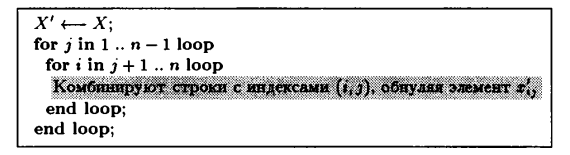
\includegraphics[width=0.8\linewidth]{image1}}
\end{figure}
... теперь должно быть более понятно, что обратимые по модулю $p^r$\linebreak
формы $a = 1 + kp$, суммы $S_{p^r}(а)$ и порядок $f$ тесно связаны между со­-\linebreak
бой. Однако, несмотря на все найденные соотнош ения, преобразование\linebreak
\newpage
$x \rightarrow 3x+1 \pmod{16}$ не является циклическим:
\begin{figure}[h]
\center{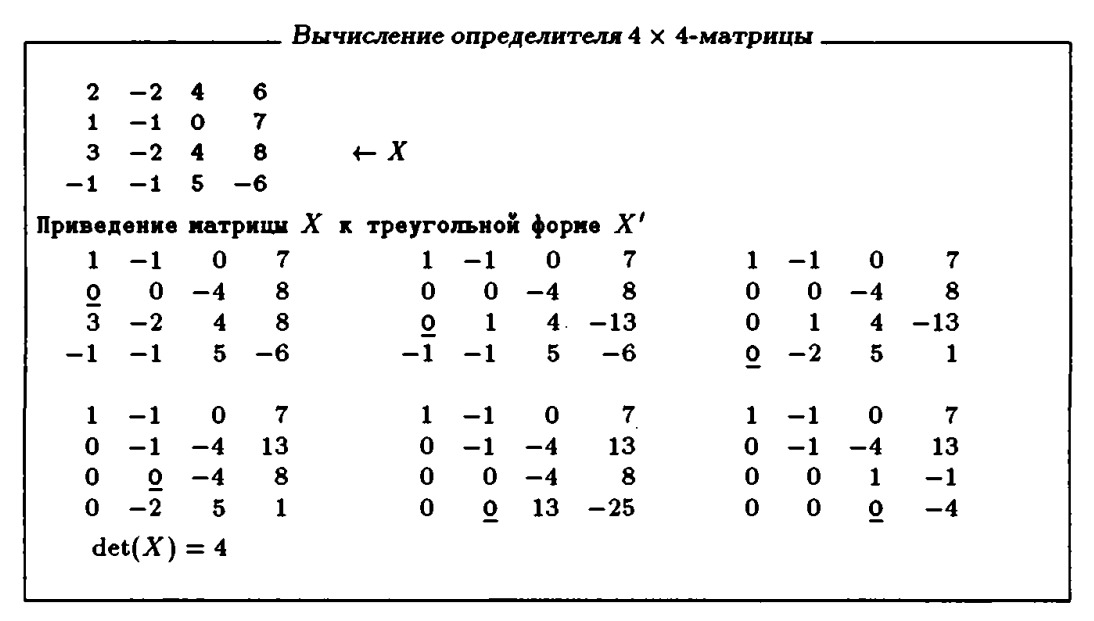
\includegraphics[width=1\linewidth]{image2}}
\end{figure}
\begin{predl}
\quad \;\;Пусть $p$ нечетное число, $k \ge 1$ и $r \ge 0$,.
\par  (\textit{i}) $x \equiv 1 \pmod{p^k} \Rightarrow S_{p^r}(x) \equiv p^r \pmod{p^{k+r}}.$
\par  (\textit{ii}) Если $x \equiv 1 + ap^k \pmod{p^{k+1}}$, то $x^{p^r} \equiv 1 + ap^{k+r}\pmod{p^{k+r+1}}$.\linebreak В частности,
$x \equiv 1 + ap \pmod{p^2}\rightarrow x^{p^r} \equiv 1 + ap^{r+1}\pmod{p^{r+2}$.}
\end{predl}
\begin{myproof}
\par (\textit{i}) Рассмотрим сначала случай $r = 1$. Тогда $x = 1 + vp^k$ для $v \in A$ и\linebreak
$$S_p(x)=1+(1+vp^k)+(1+vp^k)+...+(1+vp^k)^{p-1}$$
$$\equiv 1 + (1+vp^k) (1+2vp^k)+ ... + (1+(p-1)vp^k) \pmod{p^{k+1}}$$
$$\equiv p + vp^k(1 + 2 + ... + p - 1) \equiv p + vp^k\frac{p(p-1)}{2} \pmod{p^{k+1}}.$$
Откуда $S_p(x) \equiv p\pmod{p^{k+1}}$, так как $p$ нечетно. Для\linebreak
произвольного $r$ доказательство ведется по индукции, ибо\linebreak
$S_{p^{r+1}}(X) = S_{p^r}(X^p)S_p(X).$
\par  (\textit{ii})Имеем:
	$$x^{2^r} - 1 = (x - 1)S_{2^r}(x)=(a2^k + \alpha2^{k+1})(a2^k + \beta2^{k+r-1}=)$$
	$$=a2^{r+k}+\alpha \beta 2^{r+2k-1}+\alpha 2^{r+k+1}(1+\beta 2^{k-1})\equiv$$
	$$\equiv2^{k+r} \pmod{2^{r+k+1}}.\quad\quad\quad\quad\quad\quad\quad\quad\quad\;\;$$
\end{myproof}
\begin{mynotice}
Результаты, полученные в этом предложении, более\linebreak
тонкие, чем в предыдущем, но опираются на то, что $p$ нечетно.\linebreak
Следующие примеры показывают, что эти результаты неверны\linebreak
для четного $p$:
$$3\equiv 1\pmod{2}, \text{ но } S_2(3) \not\equiv 2 \pmod{4},$$
$$p = 2, x = 3, k = 1, r = 1;$$
$$(1 + 2)^2 \not\equiv 1 + 2^2\pmod{2^3}, p = 2, a = 1, k = 1, r = 1.$$
\end{mynotice}
\begin{beznomera}
\noindent \textbf{Применение}

Применим некоторые простые следствия предыдущего предложения\linebreak
к изучению структуры $U(\mathbb{Z}_{3^r})$. Итак, $р = 3$ и $а = - 1$. Тогда

Следовательно, $—2$ является элементом порядка $3^{r-1}$ по модулю $3^r$ . По­\linebreak
рядок $U(\mathbb{Z}_{3^r})$ равен $\phi (3^r) = 2 \times 3^{r-1}$, а значит, $—2$ не может быть\linebreak
элементом максимального порядка. Посмотрим, что дают предыдущие\linebreak
равенства для $2$ (хотя и без вычислений ясно, что $—1$ не является сте­-\linebreak
пенью $—2$):
$$(-2)^{3^{r-2}} = (1+ ap)^{3^{r-2}} \equiv 1 - 3^{r-1} \pmod{3^r}$$
$$\text{ и }$$
\noindent откуда, благодаря предложению 25, следует, что $2$ — образующий груп-\linebreak­
пы обратимых по модулю $3^r$ элементов.
\end{beznomera}
\begin{predl}
Пусть $r$ и $k$ — два целых числа, причем $k$ больше или равно 2.
\par (\textit{i}) Если $x \equiv 1 \pmod{2^k}$, то $S_{2^r}(x) \equiv 2^r \pmod{2^{k+r-1}}$. В частности,\linebreak
если $x \equiv 1 \pmod{4}$, то $S_{2^r}(x) \equiv 2^r \pmod{2^{r+1}}$.
\par (\textit{ii}) Если $x \equiv 1 + a2^k \pmod{2^{k+1}}$, то $x^{2^r} \equiv 1 + a2^{k+r+1}$.\linebreak
В частности, если $x \equiv 1 + 4a \pmod{8}$, то $x^{2^r} \equiv 1 + a2^{r+3}$.
\end{predl}
\begin{myproof}
\par (\textit{i}) Для $r = 1$ запишем $x = 1 + v2^k$, откуда $S_2(x) = 1 + (1+v2^k)$,\linebreak
что доказывает результат. Дальнейшее доказательство производится\linebreak
индукцией по $r$. Так как $S_{2^{r+1}}(x)= S_{2^{r}}(x^2)S_2(x)$=, то 
$$S_{2^{r+1}}(x)=(2^r+\alpha 2^{k+r-1}(2+\beta 2^{k})\equiv 2^{r+1},$$
ибо $r + 2k -1 \ge k + r$.
\par (\textit{ii})Имеем:
$$x^{2^r} - 1 = (x - 1)S_{2^r}(x) = (a2^{k} + \alpha 2^{k+1})(2^r+\beta 2^{k+r-1})=$$
$$= a2^{r+k}+\alpha \beta 2^{r +2k -1} + \alpha 2^{k+r+1}(1+\beta 2^{k-1})\equiv$$
$$\equiv a2^{k+r}\pmod{2^{k+r+1}},$$
ибо $r+2k-1\ge k + r +1$ (для $k \ge 2$).
\end{myproof}
\newpage
\noindent\textbf{Пример}

Пусть имеется рекуррентная последовательность
$$x_{n+1} = 13x_n + 1 \pmod{2^r}.$$
Применяя предыдущее предложение с $x = 13 \equiv 1 \pmod{4}$, находим, что\linebreak
$S_{2^{r-1}}(13) \equiv 2^{r - 1} \pmod{2^r}$, в то время как $S_{2^r}(13) =\equiv 0 \pmod{2^r}$. Это\linebreak
означает, что аффинное отображение $x \rightarrow 13x+1 \text{ mod } 2^r$ в точности\linebreak
порядка $2^r$. Это хорошо видно на следующем примере:
\begin{figure}[h]
\center{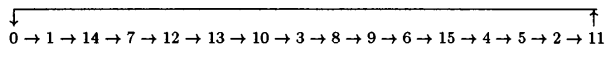
\includegraphics[width=1\linewidth]{image5}}
\end{figure}

Вопрос в том,всегда ли верно, что отображение порядка $2^r$ на $2^r$\linebreak
элементах является циклом длины $2^r$ ? Отображение $(1) (23) (456)$ пере­-\linebreak
ставляет $6$ элементов, имеет порядок $6$, но не является циклом!
\paragraph{3.4.2 Группа обратимых элементов $\mathbb{Z}/2^r\mathbb{Z}$}
\begin{thm}
\par\quad\;\;(\textit{i}) Группа $U(\mathbb{Z}_{2^r}$имеет порядок $2^{r-1}$. Группа $U(\mathbb{Z}_2)$ тривиальна,\linebreak
группа $U(\mathbb{Z}_4)$ — циклическая порядка $2$ и порождена элементом $3 = — 1$.
\par  (\textit{ii}) Предположим, что $r\ge2$. Пусть $\pi$ — отображение $U(\mathbb{Z}_{2^r})$  в\linebreak
$U(\mathbb{Z}_{4})$, определенное по правилу $\pi(x) = x\pmod{4}$. Тогда ограничение $\pi$ на\linebreak
$\{ — 1,1\}$ — изоморфизм на $U(\mathbb{Z}_4)$ и имеется разложение\linebreak
$U() = \text{Ker }\pi  х {—1, 1}$, которое задается следующим образом:
$$x = x \times 1, \text{ если } x \equiv 1 \pmod{4},$$
$$x = (-x) \times (-1), \text{ если } x \equiv 3 \pmod{4}$$
Кроме того, $\ker\pi$ - циклическая группа порядка $2^{r-2}$.
\par  (\textit{iii}) Предположим,что $r > 2$. Пусть $x = 1\pmod{4}$. Тогда\linebreak
$x\pmod{2^r}$ является порождающим $\text{Ker }\pi$ тогда и только тогда, когда\linebreak
$x\not\equiv 1 \pmod{8}$. Например, $5$ — образующий $\text{Ker }\pi$ по модулю $2^r$ для\linebreak
всякого $r\ge2$ (как мы это видели в разделе 1).
\par  Итак, при $r > 2$ группа $U(\mathbb{Z}_{2^r})$ порядка $2^{r-1}$ является прямым произ­-\linebreak
ведением циклической группы порядка $2^{r-2}$, порожденной элементом $5$,\linebreak
и циклической группы порядка $2$, порожденной элементом $—1$.
\end{thm}
\pagebreak
\begin{myproof}
\par  (\textit{ii}) То, что $\Ker{\pi}$ циклическая, следует из пункта (\textit{iii}) при $r > 2$\linebreak
и из того, что $\pi$ --- изоморфизм при $r = 2$.
\par  (\textit{iii}) Пусть $x$ — такое целое число, что $x \equiv 1 (\text{mod } 4)$. Обозна­-\linebreak
чим через $\overline{x}$ его класс по модулю $2^r$ и запишем $x = 1 + 4a$ с
$a \in \mathbb{Z}$. Так как $x$ принадлежит группе $\Ker{\pi}$, порядок которой равен\linebreak
$2^{r-2}$, то $x^{2^{r-2}} \equiv 1 (\text{mod } 2^r)$. Кроме того, согласно предложению 32,\linebreak
$x^{2^{r-3}} \equiv 1 + a2^{r-1} (\text{mod } 2^r)$ и, следовательно, $x^{2^{r-3}} \not\equiv 1 (\text{mod } 2^r)$ то­-\linebreak
гда и только тогда, когда $a \not\equiv 0 (\text{mod } 2)$. Это означает, что порядок\linebreak
$x$ равен $2^{r-2}$ тогда и только тогда, когда $x \not\equiv 1 (\text{mod }8)$.
\end{myproof}
\paragraph{3.4.3 Группа обратимых элементов	$\mathbb{Z}/p^r\mathbb{Z}$ при нечетном $p$}
%\newtop{Группа обратимых элементов	$\mathbb{Z}/p^r\mathbb{Z}$ при нечетном $p$}
\begin{lemma}
Предложение 30 (\textit{ii}) позволяет определить отображение $\chi_{r,k}$ из\linebreak
$U(\mathbb{Z}_{p^r})$ в $U(\mathbb{Z}_{p^{r+k}})$ по правилу $\chi_r,k(x mod р^{r+k}) = x^{p^k}\text{mod }р^{r + k}$. Позво-­\linebreak
ляя себе небольшую вольность, будем это иногда обозначать через\linebreak
$\chi_{r,k}(x)=x^{p^k}$.
\end{lemma}
\begin{predl}
Пусть $\pi$ — естественный гомоморфизм $U(\mathbb{Z}_{p^r})$ на $U(\mathbb{Z}_p)$. Обозначим\linebreak
через $\chi = \chi_{1,r-1}$ отображение из $U(\mathbb{Z}_p)$ в $(U(\mathbb{Z}_{p^r})$.
 
\par  (\textit{i}) Отображение $\chi$ есть сечения $\pi: \pi \textopenbullet \chi = Id$. В частности, $\chi$ инъ-\linebreak
ективно, а $\pi$ сюрьективно.
\par  (\textit{ii}) Благодаря разложению $x = {(x^{p^{r-1}})^{-1}} \times x^{p^{r-1}}$, имеем $U(\mathbb{Z_{p^r}})=$$\ker\pi \times \im \chi.$
\par  (\textit{iii}) Кроме того $\ker \pi$ --- группа порядка $p^{r-1}$, состоящая из таких\linebreak
элементов $x \in U(\mathbb{Z}_{p^r})$, что $x \equiv 1 (\mod p)$, a $\im x$ — группа порядка\linebreak
$p — 1$, образованная $q$-ми степенями элементов из $U(\mathbb{Z}_{p^r})$, где $q = p^r - 1$\linebreak
($\im x$ изоморфна $U(\mathbb{Z}_p)$).
\end{predl}
\begin{myproof}
 
\par  (\textit{i}) Пусть $x \in \mathbb{Z} - p\mathbb{Z}$, т.е. $x$ обратимо по модулю $p^k$ для любого $k$.\linebreak
Тогда
$$\pi \textopenbullet \chi(x\mod p) = \pi (x^{p^{r-1}}\mod p^r)=^{p^{r-1}}\mod p=x\mod p,$$
$$\text{так как } y^p \equiv y (\mod p).$$
\newpage
\par  (\textit{ii}) Отображение $r = 
\chi \textopenbullet \pi$ является проекцией $U(\mathbb{Z}_{p^r})$, т.е. $r \textopenbullet r = r$.\linebreak
Следовательно, имеем классическое разложение в прямое произве-\linebreak­
дение ядра и образа:
$$U(\mathbb{Z}_{p^r})=\text{Ker }r \times \im r, \text{ по правилу: }x = (xr(x)^{-1})\times r(x)$$
То, что разложение $\text{Ker }r \times \im r$имеет место и что оно единственно,\linebreak
сразу следует из свойства $r \textopenbullet r = r$. В нашем случае $\chi$ инъективно,\linebreak
а значит, $\text{Ker }r = \text{Ker } \pi$, а так как $\pi$ сюръективно, то $\im r= \im \chi$.\linebreak
Вычисляя $x * r (x)^{-1}$ и $r(x)$, получим выражения, записанные в усло­-\linebreak
вии.
\par  (\textit{iii}) $\text{Ker }\pi$ состоит из элементов $U(\mathbb{Z}_{p^r})$ таких, что $x \equiv 1 (\mod р)$, и\linebreak
нетрудно сосчитать количество таких элементов: $p^{r - 1}$ . Таким обра-\linebreak
зом, снова получили функцию Эйлера для $p^r$.
\end{myproof}
\begin{predl}
Пусть $p$ --- нечетное простое число, а $r > 0$.
 
\par  (\textit{i}) Элемент $1 - p$ имеет порядок $p^{r-1}$ в $\text{Ker }\pi$. Другими словами, $1-p$\linebreak
порождает $\text{Ker }\pi$.
\par  (\textit{ii})Гомоморфизм $\chi_{r,k}$ группы $U(\mathbb{Z}_{p^r})$ инъективен.
\end{predl}
\begin{myproof}
 
\par  (\textit{i}) Порядок $\text{Ker }\pi$ равен $p^{r-1}$ и, очевидно, $1 — p$ принадлежит $\text{Ker }\pi$.\linebreak
Следовательно, порядок $1 — p$ делит $p^{r - 1}$. Кроме того, используя\linebreak
предложение 31 (i), имеем:
$$(1-p)^{p^{r-2}}\equiv 1 - p^{r-1} \not\equiv 1 (\mod p^r).$$
Значит, $1 - p$ имеет порядок $p^{r-1}$.
\par  (\textit{ii}) Достаточно доказать, что инъективен $\chi_{r,1}$. Действительно,\linebreak
$$\chi_{r,k} = \chi_{r+k-1,1}\textopenbullet...\textopenbullet\chi_{r+1,1}\textopenbullet\chi_{r,1}.$$
Для этого же достаточно показать, что из $x^p \equiv 1 (\mod p^{r+1})$ сле­-\linebreak
дует $x \equiv 1 (\mod p^r)$. Пусть $x$ таково, что $x^p \equiv 1(\mod p^{r + 1})$. Тогда\linebreak
$x^p \equiv 1 (\mod p)$, а значит, $x \equiv 1 (\mod p)$. Согласно предложению 31\linebreak
(i) имеем $S_p(x) = p (\mod p^2 )$ и тем более $S_p (x) \not\equiv 0 (\mod p^2 )$. Из\linebreak
равенства $x^p -1 = (x - 1)S_p(x)$ и того, что по условию левая часть\linebreak
равенства делится на $p^{r + 1}$ , a $S_p(x)$ не делится на $p^2$ по только что
доказанному, заключаем, что $r —1$ делится на $p^r$. Что и требовалось
доказать.
\end{myproof}
\begin{mynotice}
Элемент $1 + kp$ также порождает $\text{Ker }\pi$, если $k \not\equiv 0$\linebreak $(\mod p)$.

Отображение $\mathbb{Z}$ в $U(
\mathbb{Z}_{p^2})$, которое каждому числу $b$ ставит в\linebreak
соответствие $1 — bp$, является гомоморфизмом, чье ядро — $p\mathbb{Z}$, а\linebreak
образ — $\text{Ker }\pi$. Это отображение индуцирует изоморфизм $\mathbb{Z}_p$ и\linebreak
$\text{Ker }\pi$. Если $x \in \mathbb{Z} — p\mathbb{Z}$, то разложение $U(\mathbb{Z}_{p^2})$, введенное в предло­-\linebreak
жении 35, позволяет записать $x = x^p(x^{p-1})^{-1}$. По малой теореме\linebreak
Ферма 
$x^{p-1}=1+a_xp$, а значит $x \equiv x^p(1-a_xp) (\mod p^2)$, откуда\linebreak
$$x \equiv x^p(1-p)^{a_x}(\mod p^2).$$
Это позволяет заключить, что в $U(\mathbb{Z}_{p^2})$ компонента $x$, принадле-\linebreak­
жащая $\text{Ker }\pi$, есть степень $a_x$ образующей $1 — p$ ядра $\text{Ker }\pi$.
\end{mynotice}

Предыдущее предложение позволяет полностью определить струк­-\linebreak­
туру $U(\mathbb{Z}_{p^к})$ для нечетного простого $P$. Так как $p — 1$ и $p^r - 1$ взаимно\linebreak­
просты и группа $U(\mathbb{Z}_{p^r})$ — прямое произведение циклических групп\linebreak­
порядков $p — 1$ и $p^r - 1$, то она изоморфна $\mathbb{Z}_{p^{r-1}(p-1)}$ и циклична.
\begin{thm}
Пусть $p$ — нечетное простое число, а $r$ - строго положительное целое число.
 
\par  (\textit{i}) Элемент $1 - p$ имеет порядок $p^{r-1}$ в $U(\mathbb{Z}/{p^r}\mathbb{Z})$.
\par  (\textit{ii}) Группа $U(\mathbb{Z}/{p^r}\mathbb{Z})$ изоморфна прямому произведению подгруппы
порядка $p^{r-1}$, порожденной элементом $1-p$, и подгруппы порядка $p — 1$,
образованной $q$-ми степенями элементов $U(\mathbb{Z}/{p^r}\mathbb{Z})$, где $q = p^{r-1}$ . Вторая
подгруппа изоморфна $U(\mathbb{Z}/{p^r}\mathbb{Z})$.
\par  (\textit{iii}) Группа $U(\mathbb{Z}/{p^r}\mathbb{Z})$ --- \textbf{циклическая} порядка $p^{r-1}(p-1)$.
\end{thm}


\noindent\textbf{Пример}
\\

В таблице 4 дана группа обратимых по модулю 125 элементов, разло­-\linebreak­
женная согласно предыдущему изложению. В первом столбце находится\linebreak­
образ $\chi$ , а в первой строке --- ядро $\pi$.

Первый столбец состоит из 25-х степеней чисел по модулю 125 и\linebreak­
изоморфен$U(\mathbb{Z}_5)$. При этом \textit{изоморфизме} элементы 57 и 68 соответ­-\linebreak­
ствуют образующим группы $%U(\mathbb{Z}_5)$. Кроме того, теперь легко опреде­-\linebreak­
лить образ любого элемента из $%U(\mathbb{Z}_125)$ под действием $\chi$:это элемент\linebreak­
первого столбца, который имеет тот же остаток по модулю 5.
\newpage
\end{document} 
\begin{mynotice} Элемент $1+kp$ также порождает $Ker$ $\pi$, если $k \not\equiv 0$ \linebreak $(mod p)$. \par

Отображение $\mathbb{Z}$ в $U({{\mathbb{Z}}_{p^{2}}})$, которое каждому числу b ставит в \linebreak соответствие $1-bp$, является гомоморфизмом, чье ядро --- $p \mathbb{Z}$, а \linebreak образ --- $Ker$ $\pi$. 
Это отображение индуцирует изоморфизм $\mathbb{Z}_{p}$ и \linebreak $Ker$ $\pi$. Если $x\in\mathbb{Z} - p\mathbb{Z}$, то разложение $U(\mathbb{Z}_{p^{2}})$, введенное в предло- \linebreak жении 35, позволяет записать $x$ = $x^{p}(x^{p-1})^{-1}$. По малой теореме \linebreak Ферма $x^{p-1}=1+a_{x}p$, а значит, $x\equiv x^{p}(1-a_{x}p) (mod \; p^{2})$, откуда \par  
\vspace{\baselineskip}
$$ x\equiv x^{p}(1-p)^{a_{x}} (mod \; p^2). $$ \par
\vspace{\baselineskip}
\noindent Это позволяет заключить, что в $U(\mathbb{Z}_{p^{2}})$ компонента $x$, принадле- \linebreak жащая $Ker$ $\pi$, есть степень $a_{x}$ образующей $1-p$ ядра $Ker$ $\pi$. \par
\vspace{\baselineskip}
\end{mynotice}
Предыдущее предложение позволяет полностью определить струк- \linebreak туру $U(\mathbb{Z}_{p^{r}})$ для нечетного простого p. Так как p - 1 и $p^{r-1}$ взаимно \linebreak просты и группа $U(\mathbb{Z}_{p^{2}})$ --- прямое произведение циклических групп \linebreak порядков $p-1$ и $p^{r-1}$, то она изоморфна $U(\mathbb{Z}_{p^{r-1}(p-1)})$ и циклична. \par
 
\vspace{\baselineskip}
\begin{thm}
\slshape{Пусть p --- нечетное простое число, а r --- строго положительное \linebreak целое число.} \par \slshape{(\textit{i}) Элемент $1-p$ имеет порядок $p^{r-1}$ в $U(\mathbb{Z}/p^{r})$.} \par 
\slshape{(\textit{ii}) Группа $U(\mathbb{Z}/p^{r}\mathbb{Z})$ изоморфна прямому произведению подгруппы \linebreak подрядка $p^{r-1}$, порожденной элементом $1-p$, и подруппы порядка $p-1$, \linebreak образованной q-ми степенями элементов  $U(\mathbb{Z}/p^{r}\mathbb{Z})$, где $q=p^{r-1}$. Вторая подруппа изоморфна  $U(\mathbb{Z}/p\mathbb{Z})$}. \par 
\slshape{(\textit{iii}) Группа $U(\mathbb{Z}/p^{r}\mathbb{Z})$ --- циклическая порядка $p^{r-1}(p-1).$}
\end{thm}
\noindent \textbf{Пример} \par
\upshape{В таблице 4 дана группа обратимых по модулю 125 элементов, разло- \linebreak женная согласно предыдущему изложению. В первом столбце находится \linebreak образ $\chi$, а в первой строке --- ядро $\pi$.} \par
Первый столбец состоит из 25-x степеней чисел по модулю 125 и \linebreak изоморфен $U(\mathbb{Z}_{5})$. При этом \textit{изоморфизме} элементы 57 и 68 соответ- \linebreak ствуют образующим группы $U({\mathbb{Z}_{5}})$. Кроме того, теперь легко опреде- \linebreak лить образ любого элемента из $U(\mathbb{Z}_{125})$ под действием $\chi$ : это элемент \linebreak первого столбца, который имеет тот же остаток по модулю 5. \par

\newpage
% новая страница 464 ---------------------------------

\begin{center}
    \begin{tabular}{| c | c | c | c | c | c | c | c | c | c | c | c | c | c }
    \hline
    \itshape{1} & \itshape{6} & \itshape{11} & \itshape{16} & \itshape{21} & \itshape{26} & \itshape{31} & \itshape{36} & \itshape{41} & \itshape{46} & \itshape{51} & \itshape{56} & \itshape{61} & ... \\ \hline
    \itshape{57} & \textbf{92} & \textbf{2} & \textbf{37} & \textbf{72} & 107 & \textbf{17} & \textbf{52} & \textbf{87} & \textbf{122} & 32 & \textbf{67} & \textbf{102} & ...
\\ \hline
    \itshape{68} & \textbf{33} & \textbf{123} & \textbf{88} & \textbf{53} & 18 & \textbf{108} & \textbf{73} & \textbf{38} & \textbf{3} & 93 & \textbf{58} & \textbf{23} & ...
\\ \hline
    \itshape{124} & 119 & 114 & 109 & 104 & 99 & 94 & 89 & 84 & 79 & 74 & 69 & 64 & ...
\\ \hline
    \end{tabular}
\end{center}

\begin{center}
    \begin{tabular}{| c | c  c | c | c | c | c | c | c | c | c | c | c | c }
    \hline
    \itshape{1} & ... & \itshape{66} & \itshape{71} & \itshape{76} & \itshape{81} & \itshape{86} & \itshape{91} & \itshape{96} & \itshape{101} & \itshape{106} & \itshape{111} & \itshape{116} & \itshape{121} \\ \hline
    \itshape{57} & ... & \textbf{12} & \textbf{47} & 82 & \textbf{117} & \textbf{27} & \textbf{62} & \textbf{97} & 7 & \textbf{42} & \textbf{77} & \textbf{112} & \textbf{22}
\\ \hline
    \itshape{68} & ... & \textbf{113} & \textbf{78} & 43 & \textbf{8} & \textbf{98} & \textbf{63} & \textbf{28} & 118 & \textbf{83} & \textbf{48} & \textbf{13} & \textbf{103}
\\ \hline
    \itshape{124} & ... & 59 & 54 & 49 & 44 & 39 & 34 & 29 & 24 & 19 & 14 & 9 & 4
\\ \hline
    \end{tabular}
\end{center}

\noindent \textbf{Таблица 4.} Разложение группы обратимых по модулю 125 элементов \par

\vspace{\baselineskip}

Первая строка представляет собой подгруппу $U(\mathbb{Z}_{125})$, изоморфную \linebreak $\mathbb{Z}_{25}$. Этот изоморфизм очень просто выражается в явном виде: он ото- \linebreak бражает элемент $x$ из $\mathbb{Z}_{25}$ в элемент $(1+5)^x$ из $U(\mathbb{Z}_{125})$, тем самым \linebreak преобразуя аддитивную структуру $\mathbb{Z}_{25}$ в мультипликативную струк- \linebreak туру подгруппы из $U(\mathbb{Z}_{125})$, образованной элементами, сравнимыми с \linebreak  1 по модулю 5. Эта подгруппа имеет 20 образующих (они выделены в \linebreak таблице курсивом). \par 
Группа $U(\mathbb{Z}_{125})$ есть прямое произведение первой строки и перво- \linebreak го столбца таблицы; ее образующие представляют собой произведения \linebreak образующих элементов из подгрупп, соответствующих первому столб- \linebreak цу и первой строке. Все образующие группы обратимых по модулю 125 \linebreak элементов выделены в таблице жирным шрифтом. Сколько же их? Не \linebreak трудно проверить, что их ровно $\varphi(\varphi(125)) = 40.$ \par
\vspace{\baselineskip}
Продолжим наше исследование. В случае $U(\mathbb{Z}_{{2}^{r}})$ мы выяснили, что \linebreak элемент 5 порождает \textit{подгруппу}  порядка $2^{r-2}$ при r > 2. Займемся те- \linebreak перь поиском примитивных корней в $U(\mathbb{Z}_{{p}^r}).$ \par

\begin{thm}
\slshape{Пусть p --- нечетное простое число. \par 
(\textit{i}) Пусть x обратимо по модулю p. Следующие утверждения экви- \linebreak валентны: \linebreak}
\indent \slshape{a) x --- примитивный корень по модулю $p^{r}$ для всякого r > 0, \linebreak \indent b)\; x --- примитивный корень по модулю $p^{r}$, \linebreak \indent c) x --- примитивный корень по модулю p и $x^{p-1} \not\equiv 1 \; ($mod$ \; p^{2}).$ } \par 
\slshape{(\textit{ii}) Пусть x --- примитивный корень по модулю p. Если $x\equiv y$ 
\linebreak $(mod \; p^{2})$ и $x \not\equiv y \; (mod \; p^{2})$, то один из элементов x или y является прими- \linebreak тивным корнем по модулю $p^{2}$. В частности, если x не является прими- } \linebreak \newpage

% новая страница 465 ----------------------------------

\noindent тивным корнем по модулю $p^{2}$, то $x+p$ и $x-p$ являются примитивными корнями по модулю $p^{2}$. 
\end{thm}
 \begin{myproof}
Импликации $a \rightarrow b \rightarrow c$ очевидны. Для доказательства $c \rightarrow a$ зап- \linebreak \indent ишем $x^{p-1} = 1 + kp$, где k не делится на p. Используя доказанные в \linebreak \indent предложении 31 (\textit{ii}) сравнения, получаем: \par 
$$x^{(p-1)p^{r-2}} \equiv 1 + kp^{r-1} (mod \; p^{r}),$$ \par 
\indent откуда следует, что порядок \textit{x} равен $(p-1)p^{r-1}$. \par 
\indent (\textit{ii}) Если $x \equiv y \; (mod \; p)$, то сформулированное в предложении 30 (\textit{ii}) \linebreak \indent соотношение приводит к $x^{p} \not\equiv y^{p} \; (mod \; p^{2})$. Остается лишь дока- \linebreak \indent зать, что $x^{p-1} \not\equiv y^{p-1} \; (mod \; p^{2})$, что равносильно $xy^{-1} \not\equiv 1 \linebreak \indent (mod \; p^{2})$. Если это не верно, то сравнение $xy^{-1} \equiv
1(mod \; p^{2})$ дава- \linebreak \indent ло бы $(xy^{-1})^{p} \not\equiv 1 \; (mod \; p^{2})$, что невозможно.
\end{myproof}
\begin{sled}
\slshape{Пусть x --- образующий группы $U(\mathbb{Z}/p^{r}\mathbb{Z})$, обратимый в $\mathbb{Z}/p\mathbb{Z}$, где \linebreak p --- нечетное простое число, $r \geqslant 1$}. Тогда остальные примитивные \linebreak корни по модулю $p^{r}$ являются степенями x, взаимно простыми с $\varphi(p^{r}) = \linebreak p(p - 1)$; их число равно $\varphi(\varphi(p^{r}))$, т.е. $p^{r - 2}(p - 1)\varphi(p - 1)$.
\end{sled}
\section{Почти периодические последовательности}
\noindent \upshape{Во многих областях математики бывает необходимо использовать так \linebreak называемые псевдослучайные последовательности чисел: в численных \linebreak методах это методы Монте-Карло, в статистике это генерирование \linebreak образцов для различных тестов, в некоторых алгоритмах требуется \linebreak выбрать \guillemotleft наугад\guillemotright \; один элемент из какого-то множества --- в этой главе \linebreak приведены конкретные примеры --- и такой случайный выбор может \linebreak значительно улучшить сложность алгоритма по отношению к выбору \linebreak детерминированному... Возникает множество вопросов относительно \linebreak так называемых \textit{генераторов случайных чисел}: насколько случайны по- \linebreak являющиеся числа? Что вообще такое последовательность случайных \linebreak чисел? Это довольно сложные вопросы.} \par 

Кнут[99] во введении к третьей граве \guillemotleft \textit{Случайные числа}\guillemotright \; своей кни- \linebreak ги, в качестве упражнения задает несколько вопросов, которые пока- \par

 \newpage


% новая страница 466 ----------------------------------

\noindent зывают, насколько наш выбор не случаен. Как, например, наугад \textit{вы- \linebreak брать} цифру от 0 до 9? Использовать телефонный справочник? Нет! \linebreak Цифры, которые там используются, неодинаково распределены. Попро- \linebreak сить кого-нибудь загадать цифру? Нет! В основном люди загадывают \linebreak вполне конкретные числа... \par 

Один из методов, используемых для образование чисел случайным \linebreak образом, состоит в применении последовательности, задаваемой срав- \linebreak нениями $x_{n+1} = ax_{n} + b \; mod \; m$. Конечно, эти последовательности на \linebreak некотором шаге становятся периодическими и нужно выбирать их так, \linebreak чтобы период был максимален. \par 

Известно, что десятичная запись рационального числа почти пе- \linebreak риодическая. Если открыть книгу, в которой изучаются непрерывные \linebreak дроби, то вскоре обнаружится, что запись непрерывной дроби действи- \linebreak тельного числа почти периодическая тогда и только тогда, когда это \linebreak число является квадратичным целым. Периодические явления встреча- \linebreak ются повсюду. В частности, всякий руррентный порцесс, происходя- \linebreak щий в конечном множестве, --- почти периодический (согласно прин- \linebreak ципу вложенных отрезков). В конце этого раздела мы увидим, что
в \linebreak некоторых случаях имеются эффективные алгоритмы для определения \linebreak периодов таких последовательностей, а в конце главы нами будет рас- \linebreak смотрен алгоритм факторизации, основанный на почти периодическом \linebreak явлении ($\rho$ -метод Полларда). \par

\subsection{Одношаговый генератор}

\noindent Случайные последовательности\footnote{Мы не будем доказывать никаких свойств этих последовательностей, касаю- \linebreak щихся их случайного ил детерминированного характера. Это выходит за рамки \linebreak данного учебника, требует серьезных статистических исследований и формального \linebreak определения того, что означает \guillemotleft наугад\guillemotright \;} легко получить при имитациях функ- \linebreak ций с одной или несколькими переменными (что влияет на длину по- \linebreak лучаемых последовательностей), выбранной таким образом, что пери- \linebreak одичность последовательностей неочевидна.

\begin{determ}
Последовательность $(x_{n})_{n}\geqslant 0$ (элементов какого-либо множества) на- \linebreak зывается периодической, если существует такое $k\geqslant 1$, что $x_{n+k} = x_{n}$ \linebreak для всех $n \in \mathbb{N}.$ Множество чисел k, удовлетворяющих этому определе- \linebreak нию, представляет собой подмножество из $\mathbb{N}^{*}$, замкнутое относитель- \linebreak но сложения и вычитания, и равное $\lambda \mathbb{N}^{*}$, где $\lambda$ --- наименьший элемент
 \newpage 
%новая страница 467 -----------------------------------
\noindent этого множества (как относительно отношения порядка $\leqslant$, так и по \linebreak делимости). \par 
Подпоследовательность $x_{0}, x_{1},..., x_{\lambda - 1}$ называется \textbf{периодом} по- \linebreak следовательности $(x_{n})_{n} \leqslant 0$, а число $\lambda$ --- \textbf{длиной периода}.
\end{determ}
\noindent\textbf{Пример} \par
\upshape{Последовательность десятичной записи числа 1/7 периодическая с \linebreak периодом длины 6, так как 1.7 = 0,\underline{142857}142857...}. Последователь- \linebreak ность $x_{n+1} = 4x_{n}, x_{0} = 5$ имеет период длины 3. Этот период \linebreak (5, 20, 17).


\begin{determ}
\slshape{Последовательность $(x_{n})_{n} \geqslant 0$} называется \textbf{почти периодической} \linebreak или \textbf{периодической некоторого ранга}, если существует такое \linebreak $m \geqslant 0$, что последовательность $(x_{n})_{n \leqslant m}$ периодическая. Обозначим че- \linebreak рез $\mu$ наименьшее из целых чисел m, удовлетворяющих этому свойству. \linebreak $\mu$ называется \textbf{индексом вхождения в период}. Назовем \textbf{периодом \linebreak последовательности} $(x_{n})_{n} \geqslant 0$ период последовательности $(x_{n})_{n \geqslant \mu}$. \linebreak Отметим, что множество \par 
{$${k \in \mathbb{N}|\exists m, x_{n+k} = x_{n}, \forall n \geqslant m},$$} \linebreak
как и в предыдущем определении, есть множество кратных длине пе- \linebreak риода.
\end{determ}
\textbf{Примеры} \par
\upshape{Последовательность $x_{n+1} = 2x_{n}+1 mod \; 48, x_{0} = 0,$ является перио- \linebreak дической ранга 4 и имеет период длины 2:} \par 
$$\;\;\;\;\;\;\;\;\;\;\;\;\;\;\;\;\;\;\;\;\;\;\;\;\;\;\;\;\;\downarrow \leftharpoonup \uparrow$$
$$0 \to 1 \to 3 \to 7 \to 15 \to 31$$ \par 
Для числа $\frac{99}{700} = 0,14\underline{142857}142857...$ последовательность десятичной \linebreak записи почти периодическая, а последовательность десятичной запи- \linebreak си $\sqrt{2} = 1,4142135623730950488016887242096980785697...$ не являет- \linebreak ся почти периодической. \par 
В данном разделе \textbf{генератором} множества F называется алго-\linebreak ритм, который выдает последовательность $(x_{n})_{n}\geqslant 0$ элементов F. На- \linebreak пример, \par 
$$x_{n+1} = 3141592521 x_{n} + 2718281829 (mod \; 10^{10}),$$
$$x_{n} = (x_{n-24}+x_{n-55})(mod \; 2^{64}),$$
$$x_{n+1} = (4x_{n}^{2} + 5x_{n})(mod \; 2^{32}).$$ \par \newpage 

%страница 468 ----------------------------------------

\noindent В дальнейшем будем считать, что $F$ \textbf{конечно}, и рассматривать только \linebreak \textbf{одношаговые} генераторы, т.е. имеющие вид $x_{n+1} = f(x_{n})$, где $f$ --- \linebreak отображение $F$ в себя. \par 
\begin{predl}
Пусть $(F,f,x_{0})$ --- генератор (множество $F$ конечно). Тогда после- \linebreak довательность $(x_{n})_{n \geqslant 0}$, определяемая по правилу $x_{n+1} = f(x_{n})$, почти \linebreak периодическая. Если $\mu$ --- индекс вхождения в период, а $\lambda$ --- длина \linebreak периода, то для различных индексов \textit{i} и \textit{j} \par

$$x_{i}=x_{j} \Longleftrightarrow \textit{i},\textit{j} \geqslant \mu и \textit{i}\equiv\textit{j} (mod \; \lambda).$$ \par 
\noindent В частности, все $x_{\textit{i}}$ при $0 \leqslant\textit{i} \leq \mu + \lambda$ попарно различны и, следователь- \linebreak но, $\mu + \lambda \leqslant|F| и \mu \leqslant|F| - 1)$. \par 
\end{predl}
\begin{myproof}
Поскольку F конечно, существую h < k такие, что $x_{h} = x_{k}$ (прин- \linebreak \indent цип ящиков). Применяя $f^{r}$, получим $x_{h+r} = x_{k+r}$, а значит, k - h --- \linebreak \indent период подпоследовательности $(x_{i})_{i}\geqslant h$. Предположим, что $x_{i} = x_{j}$ \linebreak \indent  для $j > i$. Последовательность $(x_{l})_{l \geqslant i}$ периодична, а потому $i \geqslant \mu$ и, \linebreak \indent следовательно, $j - i \equiv 0 (mod \; \lambda)$. Обратное очевидно, так же как и \linebreak \indent конец предложения. \par 
\end{myproof}
\begin{figure}[h]
\center{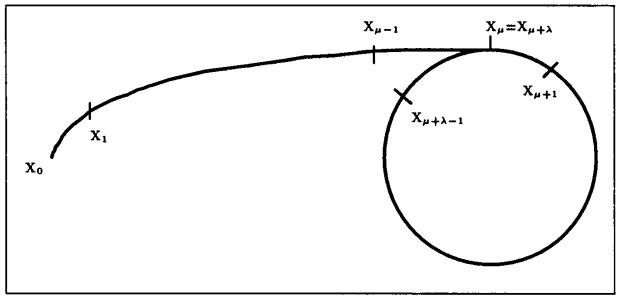
\includegraphics[width=0.8\linewidth]{image3}}
\end{figure}

Почти периодическая последовательность, получаемая при одноша- \linebreak говом генерировании, схематически может быть представлена фигурой \linebreak $\rho$(рис. 1): все элементы на $\rho$ различны, хвост --- это множество членов \linebreak \newpage

%новая страница 469-----------------

\noindent последовательности, которые не входят в период, а завиток предста- \linebreak вляет собой пеирод. Число $\mu$ является длиной хвоста, а $\lambda$ --- длиной \linebreak завитка. \par 
\vspace{\baselineskip}
\noindent \textbf{Пример: представление рационального числа в виде \linebreak десятичной дроби}
\upshape{Пусть $u$ и $v$ --- два целых числа с $v > 0$ и $q_{0} + (0 \cdot q_{1}q_{2}...)_{10}$ --- де- \linebreak сятичная запись числа $u / v$ с $q_{0} \in \mathbb{N}$. Можно определить последователь- \linebreak ность $({r_{i}})_{i \geqslant 0}$ по правилу: $r_{0} = u, r_{i+1} = 10r_{i} mod v$. Тогда $q_{i+1} = [\frac{10r_{i}}{v}]$ \linebreak (и $q_{0} = [u / v]$). Последовательность $r_{i}$ порождается с функцией $f:[0, v[ \to$ \linebreak $[0, v[$, которая каждому x ставит в соответствие $10 x mod v$. Такая по- \linebreak следовательность почти периодическая, а потому почти периодической \linebreak является и последовательность $q_{i}$ десятичных цифр в записи $u / v$.} \par 
\begin{mynotice}Отметим, что индекс вхождения в период и длина \linebreak \indent периода зависят от первого члена $x_{0}$. Например, для последова- \linebreak \indent тельности $x_{n+1} = 2x_{n} + 1 (mod 48)$ имеем: \linebreak
 
$\;\;\;\;\; \downarrow \leftharpoonup \uparrow$ \linebreak
\indent $(i)$ при $x_{0} = 0: 0 \to 1 \to 3 \to 7 \to 15 \to 31$, а значит, $\mu = 4, \linebreak \lambda = 2,$ \par 

$(ii)$ при $x_{0} = 11: 11 \to 13 \to 47 \to$ и уже $\mu = 2, \lambda = 1.$ \par 

Хотя одношаговый генератор не может порожать последо- \linebreak \indent вательности, период которых больше порядка F, очевидно, су- \linebreak \indent ществуют почти периодические последовательности произвольно \linebreak \indent большого периода. Например, для F = {0,1} последовательность \linebreak \indent $(x_{n})_{n \geqslant 0}$ такая, что $x_{n} = 0$ при $n \not\equiv 0 (mod \lambda)$ и $x_{n} = 1$ при \linebreak \indent $n \equiv 0 (mod \lambda)$ имеет период длины $\lambda$. Так как для $\lambda = 5$ получаем \linebreak \indent 0000100001.... \par 
Предыдущий пример тривиален, а потому приведем еще один \linebreak пример: \par 
\noindent $1 \, \to \, 1 \, \to \, 0 \, \to \, 1 \, \to \, 0 \, \to \, 1 \, \to \, 0 \, \to \, 0 \, \to \, 0 \, \to \, 0 \, \to \, 0 \, \to \, 1 \, \to \, 0 \, \to \, 0 \, \to \, 1$ \linebreak
$\uparrow \;\;\;\;\;\;\;\;\;\;\;\;\;\;\;\;\;\;\;\;\;\;\;\;\;\;\;\;\;\;\;\;\;\;\;\;\;\;\;\;\;\;\;\;\;\;\;\;\;\;\;\;\;\;\;\;\;\;\;\;\;\;\;\;\;\;\;\;\;\;\;\;\;\;\;\;\;\;\;\;\;\;\;\;\;\;\;\;\;\;\;\;\;\;\;\;\;\;\;\;\;\;\;\;\;\;\;\;\;\;\;\;\;\;\;\;\;\;\;\;\;\;\;\;\;\;\downarrow$ \linebreak
$ 1 \;\;\;\;\;\;\;\;\;\;\;\;\;\;\;\;\;\;\;\;\;\;\;\;\;\;\;\;\;\;\;\;\;\;\;\;\;\;\;\;\;\;\;\;\;\;\;\;\;\;\;\;\;\;\;\;\;\;\;\;\;\;\;\;\;\;\;\;\;\;\;\;\;\;\;\;\;\;\;\;\;\;\;\;\;\;\;\;\;\;\;\;\;\;\;\;\;\;\;\;\;\;\;\;\;\;\;\;\;\;\;\;\;\;\;\;\;\;\;\;\;\;\;\;\;\; 0$ \linebreak
$\uparrow \;\;\;\;\;\;\;\;\;\;\;\;\;\;\;\;\;\;\;\;\;\;\;\;\;\;\;\;\;\;\;\;\;\;\;\;\;\;\;\;\;\;\;\;\;\;\;\;\;\;\;\;\;\;\;\;\;\;\;\;\;\;\;\;\;\;\;\;\;\;\;\;\;\;\;\;\;\;\;\;\;\;\;\;\;\;\;\;\;\;\;\;\;\;\;\;\;\;\;\;\;\;\;\;\;\;\;\;\;\;\;\;\;\;\;\;\;\;\;\;\;\;\;\;\;\;\downarrow$ \linebreak
\noindent $0 \, \to \, 1 \, \to \, 1 \, \to \, 0 \, \to \, 0 \, \to \, 0 \, \to \, 1 \, \to \, 1 \, \to \, 1 \, \to \, 1 \, \to \, 1 \, \to \, 0 \, \to \, 0 \, \to \, 1 \, \to \, 1$ \linebreak

\indent В данном случае используется множество {0,1} и если приc- \linebreak мотреться повнимательнее, то видно, что все 5-ти битовые цепи \linebreak возникают в данной диаграмме ровно по одному разу. Этот цикл \linebreak длины 32, а значит, генерируется за 5 шагов. Этому циклу отве- \linebreak чает многочлен степени 5, неприводимый над $\mathbb{Z}_{2}$, $P = X^{5} + X^{5} + 1$.
\end{mynotice}
\newpage

%новая страница 470-----------------------------------------------

\begin{determ} 
\textit{Одношаговый генератор $(F,f,x_{0})$ называется генератором \textbf{максимального периода}, если длина его периода равна |F|}.
\end{determ}
\begin{predl}
\slshape{Для одношагового генератора (F,f) эквивалентны следующие усло- \linebreak вия:} \par 
\upshape{a)$(F,f,x_{0})$ максимального периода для $x_{0} \in F$. \par 
\indent b)Отображение f --- циклическая перестановка F. \par
\indent c)$(F,f,x)$ максимального периода для всех $x \in F$. \par
\indent d)Для любых $x,y \in F$ существует $r \in \mathbb{N}$ такое, что $f^{r}(x) = y.$ \par}
\indent Из двух генераторов $(F,f,x_{0})$ и $(G,g,y_{0})$ можно получить третий, \linebreak рассматривая их декартово произведение $(F \times G, f \times g, (x_{0}, y_{0})).$
\end{predl}
\begin{predl}
 \slshape{Декартово произведение двух генераторов имеет период длины, \linebreak равной НОК длин периодов компонент, а индекс вхождения, равный \linebreak наибольшему из индексов компонент.}
\end{predl}
\begin{myproof}
 Для последовательности $(u_{n})_{n \geqslant 0}$ обозначим: \par 
 $$I_{u} = {s \equiv \mathbb{N}|\exists k_{0}, u_{k+s} = u_{k}, \forall k \geqslant k_{0}}.$$ \par 
 Тогда для последовательностей $(x_{n})_{n \geqslant 0}, (y_{n})_{n \geqslant 0}, (z_{n})_{n \geqslant 0},$ порожда- \linebreak \indent емых соответственно функциями $f, g$, и $f \times g$, имеем $I_{x} \bigcap I_{y} = I_{z}$, \linebreak \indent откуда легко получить утверждение, касающееся длины периода. \linebreak \indent Последовательность $(z_{i})_{i \geqslant q}$ периодична тогда и только тогда, когда \linebreak \indent такими же являются последовательности $(x_{i})_{i \geqslant q}$ и $(y_{i})_{i \geqslant q}$, до- \linebreak \indent казывает утверждение относительно индекса вхождения в период. \par 
\end{myproof}
\subsection{Генерирование при помощи линейных сравнений}

\noindent В данное пункте рассматриваются генераторы вида \par 
$$x_{n+1} = ax_{n} + b mod \; m;$$ \par
\noindent назовем их линейными генераторами сравнений. Такие генераторы ха- \linebreak рактеризуются модулем m, \textit{аффинным} преобразованием $x \to ax + b$ кольца $\mathbb{Z}_{m}$ (назовем a мультипликатором, а b приращением) и, нако- \linebreak нец, первым членом $x_{0} \in \mathbb{Z}_{m}$. \par \newpage 

%новая страница 471----------------------

\textbf{Несколько примеров} \begin{itemize}
\item $x_{n+1} = 4x_{n}+1 \; mod \; 9, x_{0} = 0$ дает 
$$0 \to 1 \to 5 \to 3 \to 4 \to 8 \to 6 \to 7 \to 2$$
\item $x_{n+1} = 2x_{n} + 1 \; mod \; 48, x_{0} = 0$ дает $0 \to 1 \to 3 \to 7 \to 15 \to 31$
\item $x_{n+1} = 3x_{n} + 1 \; mod \; 20, x_{0} = 0$ дает $0 \to 1 \to 4 \to 13$
\item $x_{n+1} = 2x_{n} + 1 \; mod \; 5, x_{0} = 0$ дает цикл $0 \to 1 \to 3 \to 2$, а при \linebreak $x_{0} = 4$ цикл длины 1: (4).
\end{itemize}
Дадим теперь необходимые и достаточные условия того, что генера- \linebreak  тор сравнений имеет максимальный период. Более детальное изучение \linebreak читатель найдет в упражнениях 37-40. \par 
\begin{predl} (китайская теорема об остатках). \par
\indent\slshape{Пусть $m = m_{1}m_{2}$, где  $m_{1}$ и $m_{2}$} --- два взаимно простых числа. Любой \linebreak генератор сравнений по модулю $m$: \par 

\begin{equation*}
(G) 
 \begin{cases}
   &\text{$z_{n+1} = (az_{n} + b) \; mod \; m$}\\
   &\text{$z_{0} = c \; mod \; m$}
 \end{cases}
\end{equation*}

\noindent есть декартово произведение генераторов по модулям $m_{1}$ и $m_{2}$: \linebreak
 
 \begin{equation*}
(G) 
 \begin{cases}
   &\text{$x_{n+1} = (ax_{n} + b) \; mod \; m_{1}$}\\
   &\text{$x_{0} = c \; mod \; m_{1}$}
 \end{cases}
\end{equation*}
 
 
\noindent В частности, длина периода (G) равна НОК длин периодов ($G_{1}$) и ($G_{2}$), \linebreak а индекс вхождения в период (G) равен наибольшему из индексов вхо- \linebreak ждения ($G_{1}$) и ($G_{2}$). \par
\end{predl} 
\begin{myproof}
Рассмотрим преобразования $f_{1}, f_{2}, f_{3}$, определенные по правилам \linebreak \indent $f_{1}(x) = ax + b \; mod \; m_{2}, f(z) = az + b \; mod \; m.$ \linebreak \indent Тогда коммутативна диаграмма \par 

$$\mathbb{Z_{m}} \to \mathbb{Z_{m}} \linebreak \indent
 \downarrow \;\;\;\;\;\;\;\;\;\;\;\;\;\;\;\; \uparrow \linebreak \indent
 \mathbb{Z_{m_{1}}} \times \mathbb{Z_{m_{2}}} \to \mathbb{Z_{m_{1}}} \times \mathbb{Z_{m_{2}}}$$ \par 
 в которой вертикальные отображения --- это китайский изомор- \linebreak \indent физм $\bar{z_{m_{1}}} \to (\bar{z_{m_{1}}}, \bar{z_{m_{2}}})$ и, следовательно, f и $f_{1} \times f_{2}$ связаны между \linebreak \indent собой. \end{myproof}
 \newpage
 
 % новая страница 472
 
После этого общего представления генераторов сравнений, займем-  \linebreak ся теми, которые имеют максимальный период. \linebreak 
\indent Предположим, что генератор $x_{n+1} = f(x_{n}) = ax_{n} + b \; mod \; m$ имеет \linebreak максимальный период (т.е. период длины m). Тогда для всякого дели- \linebreak теля $p \geqslant 2$ числа m генератор $x \mapsto ax + b \; mod \; p$ также имеет период \linebreak длины p. Действительно, если f --- цикл на множестве A, а $\pi$ ---сюръ- \linebreak екция A на множество B, то преобразование g множества B такое, что \linebreak $\pi \circ f = g \circ \pi$, также является циклом. Поэтому, если последовательность \linebreak имеет максимальную длину, то уравнение $x = ax + b \; mod \; p$ не имеет ре- \linebreak шений для любого делителя p числа m. В частности, если p --- простое, \linebreak то: \par
$$a - 1 \equiv 0 \; (mod \; p) и\; b \not\equiv 0 \; (mod \; p).$$ \par 
\noindent Кроме того, если 4 делит m, то $a \equiv 1 (mod \; 4)$. Действительно, $a \equiv 1 \linebreak (mod \; 2)$  и условие$ a \equiv -1 (mod \; 4)$ невозможно, так как тогда \linebreak $x_{n+1} = -x_{n} + b \; mod \; 4$. Эти условия являются и \linebreak достаточными, как это следует их следующей теоремы. \par 

\begin{thm}
\textit{Генератор сравнений $x_{n+1} = f(x_{n}) = ax_{n} + b \; mod \; m$ имеет максимальный период тогда и только тогда, когда выполняются следующие \linebreak три условия:} \par 
a) b обратимо по модулю m, \linebreak
\indent b) $a \equiv 1 (mod \; p)$ для любого простого p, делящего m, \linebreak
\indent c) если 4 делит m, то $a \equiv 1 (mod 4).$ \par
\end{thm}
\begin{lemma}
Пусть f(x) = ax + b рассматривается как отображение $Z_{m}$ в себя. \linebreak Тогда q-я степень f это афинное преобразование $x \to a^{q}x + bS_{q}(a)$, \linebreak $S_{q}(X)$ --- многослен из раздела 3.4.1. В частности, если b обратимо по \linebreak модулю m, то \par
$$f^{q}(0) = 0 \Leftrightarrow S_{q}(a) = 0 \Leftrightarrow f^{q} = Id_{\mathbb{Z_{m}}}.$$ \par
\end{lemma}
\upshape{Чтобы доказать эту лемму, достаточно заметить, что $bS_{q}(a) = 0$ \linebreak эквивалентно $S_{q}(a) = 0$, так как b обратимо по модулю m, и что \linebreak $S_{q}(a) = 0$ влечет $a^{q} = 1$, ибо $a^{q} - 1 = (a - 1)S_{q}(a).$
\begin{lemma}
\slshape{Пусть p --- простое, $r \geqslant 1 (с r = 1$ при $p = 2), a \equiv 1 (mod \; p)$ и $b \not\equiv 0 \linebreak (mod \; p).$ Тогда $x \mapsto f(x) = ax + b$ --- циклическая перестановка $\mathbb{Z_{p^{r}}}$, а \linebreak значит, генератор максимального периода.}  \par \newpage 
\end{lemma}
%новая страница 473--------------------------------------------
\begin{myproof}
Отображение f это перестановка $Z_{p^{r}}$, так как a обратимо по моду- \linebreak \indent лю $p^{r}$. Кроме того, лемма тривиальна, если $p = 2$(так как r = 1). \linebreak \indent Предположим, что $p \ne 2$, и рассмотрим ограничение f на орбиту 0, равную \linebreak \indent ${f^{q}(0), q \equiv \mathbb{N}}$. Достаточно доказать, что наименьшее q та- \linebreak \indent кое, что $f^{q}(0) = 0$, равно $p^{r}$. Так как $a \equiv 1 (mod \; p)$, то $S_{p^{r}}(a) \equiv 0 \linebreak \indent (mod \; p^{r})$ согласно предложению 31, имеем $S_{p^{r}}(a) \not\equiv p^{l} (mod \; p^{l + 1})$ и, следова- \linebreak \indent тельно, $S_{p^{l}}(a) \not\equiv 0 (mod \; p^{r})$. Теперь осталось применить лемму 48.
\end{myproof}
\begin{lemma}
\slshape{Пусть $r \geqslant 2$, а $a \equiv 1 (mod \; 4)$ и $b \not\equiv 0 (mod \; 2)$. Тогда $x \mapsto f(x) = \linebreak ax + b$ --- циклическая перестановска $\mathbb{Z_{2^{r}}}$, а значит, генератор макси- \linebreak мального периода.}
\end{lemma}
\begin{myproof}
 \indent\upshape{Доказательство аналогично доказательству предыдущей леммы и \linebreak \indent использует главным образов то, что $a \equiv 1 (mod \; 2^{2})$. Согласно \linebreak \indent предложению 32 имеем $S_{p^{r}}(a) \equiv 0 (mod \; 2^{r})$, а кроме того, при \linebreak \indent $l < r, S_{2^{l}}(a) \equiv 2^{l} (mod \; 2^{l+1})$, по предложению 32, откуда $S_{2^{l}}(a) \not\equiv 0 \linebreak \indent (mod \; 2^{r})$. Затем применим лемму 48.} \par 
\end{myproof}
Теперь можно доказать теорему 47. Необходимость доказана перед \linebreak формулировкой теоремы, а достаточность следует из китайской тео- \linebreak ремы об остатках и двух предыдущих лемм. \par 
\textbf{Пример} \par
Пусть $m = 10^{6} - 1 = 3^{3} \times 7 \times 11 \times 13 \times 37$. Чтобы получить генератор \linebreak $x_{n+1} = ax_{n} + b \; mod \; m$  максимального периода, нужно выбрать (согласно \linebreak теореме 47): \par 
$$a \equiv 1 (mod 3 \times 7 \times 11 \times 13 \times 37) и b \not\equiv 0 (mod \; p)$$
$$для p \in \{3, 7, 11, 13, 37\}.$$
\noindent Это дает 9 решений для $a$ вида $1 + 111111 \times с 0 \geqslant k \geqslant 8.$
\subsection{Нахождение периода методом Брента}
\noindent Пусть f --- конечно множество, $x_{0} \in F$ и $f: F \to F$ отображение, которому соответствует последовательность $x_{n+1} = f(x_{n})$, начинаю- \linebreak щаяся с $x_{0}$. Цель алгорима Брента --- сосчитать длину периода после- \linebreak довательности $((x_{n})_{n \geqslant 0}$, используя при этом как можно меньше памяти \linebreak

% новая страница 474 ------------------------------------------

\noindent(достаточно 3 переменных!). Сложность алгоритма имеет порядок ква- \linebreak дратного корня из F.} \par 

\slshape{\textbf{Принцип метода}} \par
\upshape{Метод Брента состоит в проверке равенства $x_{h} = x_{k}$ для пар ин- \linebreak дексов (h,k), принимающих следующие значение:} \par
\begin{figure}[h]
\center{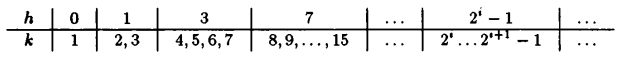
\includegraphics[width=1\linewidth]{image4}}
\end{figure}% таблица
Отметив, что для $h = 2^{i} - 1$ интервал соответствующих значений k равен $[h + 1, 2h + 1]$. Для того, чтобы теперь $x_{h} = x_{k}$, необходимо
\begin{wrapfigure}{i}{0.5\textwidth}
\begin{lstlisting}[mathescape=true]
$j \leftarrow 1; x \leftarrow x_0;j - 1 = h$
$\text{loop}$
 $x' \leftarrow{x};$
 $j \text{ - степень } 2,\text{ } x' = x = x_{j-1}$
 $\text{for }\lambda \text{ in } 1..j \text{ loop } j - 1 + \lambda = k$
  $x\leftarrow f(x); x = x_{j-1+\lambda}$
  $x'={x'} \text{ then}$
  $\text{return } \lambda;\text{ длина периода}$
  $\text{end if};$
 $\text{end loop};$
 $j\leftarrow 2j;$
$\text{end loop};$
\end{lstlisting}
Алгоритм 4. Вычисление\\
периода по методу Брента
\end{wrapfigure}
 и достаточно, чтобы $h \geqslant \mu$ (индекс вхождения в период) и k - h было  кратно $\lambda$ (длина периода) --- условия, которые выполняются при достаточно большом h (так как интервал для k удваивается на каждом этапе). Пусть h --- какой-либо индекс, для которого существует  $k \in [h + q, 2h + 1]$ с $x_{h} = x_{k}$. Если k --- первый индекс интервала $[h + q, 2h + 1]$, для которого $x_{h} = x_{k}$, то k - h равно длине периода $\lambda$. Наконец, если $\mu$ --- наименьший индекс, такой, что $x_{\mu} = x_{\mu + \lambda}$, то $\mu$ --- индекс вхождения в пеирод. Это приводит к алгоритму, представленному слева. В этом алгоритме переменная j принимает значения h + 1, т.е. степени 2. Хотя алгоритм 4 находит только длину периода, дальнейшее применение метода Брента позволяет определить все 4 параметра $(h, k, \mu, \lambda)$, описанных выше (причем $k - h = \lambda$): сложность измеряется при помощи параметра k, который равен числу итераций $x \leftarrow f(x)$ и обозначается $k_{f,x_{0}}$. \par 

\noindent\slshape{\textbf{Пример}} \par 
\upshape{Применяя метод Брента к десятичной записи числа $\frac{1}{7^{2}}$, получаем:} \par 
$$\frac{1}{49} = 0.\underline{020408163265306122448979591836734693877551}020408163...$$ \par 
\indent Длина периода равна 42 и в этом нет ничего удивительного, так как при \linebreak получении цифр десятичной записи используется функция \linebreak\newpage 

% новая страница 475--------------------------------------------

\noindent$x \mapsto 10x \; mod]; 7^{2}$ и длина периода равна порядку элемента 10 в суль- \linebreak типликативной группе $U(\mathbb{Z^{7_{2}}})$. Но 10 --- порождающий элемент \linebreak группы $U(\mathbb{Z^{7_{2}}})$ и $10^{7-1} \not\equiv 1 (mod \; 7^{2})$, а значит, 10 --- порождающий элемент \linebreak группы $u(\mathbb{Z^{7_{2}}})$ и его порядок $\phi(7^{2}) = 42$. \par 

\noindent\slshape{\textbf{Сложность метода Брента}} \par 
\upshape{Рассмотрим теперь следующую проблему: если f --- функция, дей- \linebreak ствующая из F в F, и начальный член $x_{0} \in F$ "выбран наугад", то \linebreak каков порядок величин $\lambda$ (длина периода), $\mu$ (индекс вхождения алгоритма в пе- \linebreak риод) и индекса $k = k_{f,x_{0}}$, полученного после применения алгоритма \linebreak Брента? Основной результат данного раздела состоит в том, что эти \linebreak величины имеют порядок $\sqrt{m}$, где m --- число элементов в F. Основ- \linebreak ные идеи доказательства заимствованы из книги Кнута "The Art Of \linebreak Computer Programming", успржнения к разделам 3.1 и 4.5.4. Читатель \linebreak может также обратиться к [104], [155] и [67].} \par 
Заметим сначала, что если $\mu$  --- индек с вхождения, то выполняется \linebreak равенство (в котором сложное выражение $2^{[log_{2}n])}$ --- это наименьшая \linebreak степень 2б большая или равная n): \par 
$$k_{f,x_{0}} = 2^{[log_{2}max(\mu+1,\lambda)]} + \lambda - 1$$ \par 
\noindent Действительно, $h = k_{f,x_{0}} - \lambda$ --- это наименьшее целое число, такое, что: \par 

$$h + 1 степень 2 и h \geqslant \mu, (2h + 1) - h \geqslant \lambda.$$ \par 
\noindent Значит h, удовлетворяющее этим условиям, равно $2^{[log_{2}max(\mu + 1,\lambda)]} - 1$, \linebreak откуда и следует равенство для $k_{f,x_{0}}$. Заметим, что $k_{f,x_{0}}$ зависит только \linebreak от $\lambda$ или $\mu$, а потому обозначим его через $k_{\mu, \lambda}$. \par 
Зафиксируем конечное множество F мощности m и рассмотрим ве- \linebreak роятностное пространнство, состоящее из возможных пар $(f, x_{0})$, где \linebreak $f: F \to F$ --- некоторая функция, а $x_{0} \in F$. \par 

\begin{lemma}
Пусть F --- конечное множество мощности m и $\lambda$, $\mu$ удовлетворяют \linebreak неравенствам $1 \geqslant \lambda \geqslant m, 0 \geqslant \mu и \mu + \lambda \geqslant m$. Вероятность того, \linebreak что последовательность $x_{n+1} = f(x_{n})$(f --- функция из F в F, $x_{0} \in F$) \linebreak имеет   период длины $\lambda$ и индекс вхождения $\mu$, равна \par 

$$P(\mu, \lambda)=\frac{1}{m} \Pi_{1\geqslant k<\mu+\lambda} (1 - \frac{k}{m}).$$ \par 
\noindent Функция $P(\mu,\lambda)$ зависит только от $\mu + \lambda$ (и m, очевидно). \end{lemma}
\newpage 
%новая страница 476--------------------------------------------

\begin{myproof}
Имеется $m^{m+1}$ возможностей выбора функции f из F в F (число \linebreak которых $m^m$) и первого члена $x_{0}$. Благоприятным исходом, кото- \linebreak \indent рому соответствует пара $(f, x_{0})$, является последовательность из \linebreak \indent $\mu + \lambda$ различных элементов $E = (x_{0}, x_{1},..., x_{\mu + \lambda -1})$(на которой f \linebreak \indent зацикливается) и произвольная функция из $F - E$ в F (сужение f \linebreak \indent на $F - E$). Число благоприятных исходов равно \par 

$$m \times (m - 1) \times ... \times (m -(\mu + \lambda - 1)) \times m^{m - (\mu + \lambda)}.$$ \par 
Значит, отношение числа благоприятных исходов к общему числу возможностей равно: \par 

$$\frac{m \times (m - 1) \times ... \times (m - (\mu + \lambda - 1))}{m^{\mu + \lambda + 1}} =$$ $$= \frac{1}{m} \times (1 \ \frac{1}{m})\times ... \times (1 - \frac{\mu + \lambda - 1}{m}).$$ \par 
\end{myproof}
\begin{determ}
\slshape{Определим функцию $Q : \mathbb{N^{*}} \to \mathbb{R^{+}}$ следующим образом \par}

$$ Q(m) = 1 + \frac{m - 1}{m} + \frac{m - 1}{m}\frac{m - 2}{m} +...+\frac{m - 1}{m}\frac{m - 1}{m}...\frac{1}{m}$$ \linebreak
$$= \sum_{1 \geqslant q \geqslant m} \Pi_{1 \geqslant k \geqslant q}(1 - \frac{k}{m}) = \sum_{1 \geqslant q \geqslant m} \frac{m!}{(m - q)!m^{q}}.$$ \par 
\noindent Она связана с $P(\mu, \lambda)$ равенством $\sum_{0 \geqslant \mu \geqslant m}P(\mu,1) = Q(m)/m.$ \par 
\end{determ}
\begin{predl}
\slshape{Кнутом в книге The Art Of Computer Programming, раздел 1.2.11.3, была получена асимптотическая формула для функции Q:} \linebreak 

$$Q(n) = \sqrt{\frac{\pi n}{2}} - \frac{1}{3} + \frac{1}{12}\sqrt{\frac{\pi}{2n}} - \frac{4}{135n} + \frac{1}{288}\sqrt{\frac{\pi}{2n^{3}}} + O(n^{-2}).$$ \par 

\upshape{Функция Q используется при изучении сложности алгоритма Брен- \linebreak та.} \linebreak
\end{predl}
\begin{lemma}
\slshape{Если индексы $\lambda$ и $\mu$ связаны соотношениями $1 \geqslant  \lambda \geqslant m, 0 \geqslant \mu < m$ \linebreak \newpage 

% новая страница 477-------------------------------------------

и $\mu + \lambda \leqslant m$, то выполняются равенства:} \par
 
$$\sum_{\mu,\lambda} P(\mu,\lambda) = \frac{1}{m} \sum_{1 \leqslant q < m} q \Pi_{1 \leqslant k < q} (1 - \frac{k}{m}) = 1,$$ \par 

$$\sum_{\mu,\lambda} (\mu + \lambda) P(\mu,\lambda) = \frac{1}{m} \sum_{1 \leqslant q < m} q^{2} \Pi_{1 \leqslant k < q} (1 - \frac{k}{m}) = Q(m),$$ \par 

$$\sum_{\mu,\lambda} \lambda P(\mu,\lambda) = \frac{1}{m} \sum_{1 \leqslant q < m} \frac{q(q+1)}{2} \Pi_{1 \leqslant k < q} (1 - \frac{k}{m}) = \frac{Q(m)+1}{2},$$ \par 

$$\sum_{\mu,\lambda} \mu P(\mu,\lambda) = \frac{1}{m} \sum_{1 \leqslant q < m} \frac{q(q-1)}{2} \Pi_{1 \leqslant k < q} (1 - \frac{k}{m}) = \frac{Q(m)-1}{2}.$$ \par

\noindent Эти равенства представляют собой математические ожидания соответ- \linebreak ственно 1, $\mu + \lambda, \lambda и \mu$. \par
\end{lemma}
\begin{myproof}
\indent Заметим, что \linebreak 
$$\sum_{\mu,\lambda} g(\mu, \lambda) P(\mu, \lambda) = \sum_{1 \leqslant q < m} \sum_{\mu + \lambda = q} g(\mu, \lambda) =$$ \par 
$$\frac{q}{m} \sum_{1 \leqslant q < m} \sum_{1 \leqslant \lambda < q} g(q - \lambda,\lambda) \Pi_{1 \leqslant k < q} (1 - \frac{k}{m}),$$ \par 

что позволяет перейти от выражений с $(\mu, \lambda)$ к выражениям с q. \linebreak \indent Функция $P(\mu, \lambda)$ была определена как вероятность и, следователь- \linebreak \indent но, $\sum_{\mu,\lambda} P(\mu,\lambda) = 1$ (первая формула леммы). \linebreak \indent
Для бесконечной последовательности $a = (a_{0}, a_{1}, a_{2},...)$ 
 определим \linebreak \indent f(a): \par 
 $$f(a) = f(a_{0}, a_{1}, a_{2},...) = \sum_{n \geqslant 0} a_{n} \Pi_{1 \leqslant k \leqslant n} (1 - \frac{k}{m}) = $$ \par
 
 $$= a_{0} + a_{1}(1 - \frac{1}{m}) + a_{2}(1 - \frac{1}{m})(1 - \frac{2}{m}) + ...,$$ \par 
 сумма, в которой лишь конечное число слагаемых не равно нулю, \linebreak \indent так как внутреннее произведение равно нулю при $n \geqslant m$. Вычислим \linebreak \indent $f(1^{2}, 2^{2}, 3^{2},...)$. Используя то, что при $n \geqslant 1$ \linebreak \indent \newpage
 
 % новая страница 478-------------------------------------------
 
 $$a_{n}(1 - \frac{1}{m})...(1 - \frac{n}{m}) = a_{n}(1 - \frac{1}{m})...(1 - \frac{n - 1}{m}) -$$ \par
 $$\frac{na_{n}}{m}(1 - \frac{1}{m})...(1 - \frac{n - 1}{m}),$$ \par 
\noindent получаем равенство: \par 
 
 $$f(a) = f( a_{0}, a_{1}, a_{2},...) = a_{0} +  f( a_{1}, a_{2}, a_{3},...) - \frac{1}{m} f( f( a_{1}, 2a_{2}, 3a_{3},...).$$ \par 
 
\noindent Для удобства обозначим $\Delta a = (a_{1} - a_{0}, a_{2} - a_{1}, a_{3} - a_{2},...)$ и $a' = (a_{1}, 2a_{2}, 3a_{3},...)$ и из предыдущего равенства получим: \par 
 
 $$\frac{a'}{m} = f(\Delta a) + a_{0}.$$ \par
 
\noindent Применяя это равенство к постоянной последовательности 1, полу- \linebreak чим $f(1,2,3,...) = m$, \noindent что доказывает первую формулу леммы. А ес- \linebreak ли применить это равенство к последовательности $a =(0,1,2,3,...),$ получим: \par 
 
 $$\frac{(1^{2}, 2^{2}, 3^{2},...)}{m} = f(1,1,1,...) + 0 = Q(m),$$ \par 
 что дает вторую формулу. Две последние формулы являются след- \linebreak ствиями первых. \par
\end{myproof}
\begin{predl} 
 \slshape{Математическое ожидание $E(k_{\mu, \lambda})$ индекса Брента оценивается сле-\linebreak дующим образом \par }
 
 $$1,5Q(m) - 0,5 \leqslant E(k_{\mu, \lambda}) \leqslant 1,625Q(m) - 0,5.$$ \par 
 \end{predl}
\begin{myproof}
 Вместо обычных индексов запишем $E(k_{\mu, \lambda}) = \sum_{\mu, \lambda} k_{\mu, \lambda}P(\mu, \lambda) = S_{1} + S_{2}$, \linebreak \indent где \par
 
 $$S_{1} = \sum_{\mu, \lambda} 2^{[log_{2} max(\mu + 1,\lambda)]} P(\mu, \lambda), \;\;\;\;\;\; S_{2} = >\sum_{\mu, \lambda}P(\mu, \lambda).$$ \par 
 
 Согласно предыдущему результату сумма $S_{2}$ равна $(Q(m) - 1)/2$. \linebreak \indent Осталось лишь вычислить сумму $S_{1}$, которую перепишем так: \linebreak \newpage 
 
%новая страница 479--------------------------------------------

$$S_{1} = \frac{1}{m} \sum{1 \leqslant q < m} f(q) \Pi {1 \leqslant k < q} (1 - \frac{k}{m}),$$ \linebreak 
$$где f(q) = \sum{1 \leqslant \lambda < q} 2^{[log_{2}max(q+1-\lambda,\lambda)]}.$$ \par 

\noindent Найдем ограничения для f(q). Значения $u = max(q + 1 - \lambda, \lambda)$ для \linebreak \noindent $1 \leqslant \lambda < q$ следующие: \par

$$u = q, q - q, ...,[q/2] + 1, ..., q - 1, q,$$ \par

\indent и значение [q / 2] + 1 для f(q) появляется два раза при четном q и один раз \linebreak \indent при нечетном. Теперь, чтобы определить f(q), нужно определить \linebreak \indent $2^{[log_{2}u]}$ для приведенных выше значений u. Пусть 2q' --- первая сте- \linebreak \indent пень 2, большая или равная q. Тогда $q' < q \leqslant 2q'$, и, в частности, \linebreak \indent $q/2 \leqslant q'$. Для значений u, удовлетворяющих условию $q' + 1 \leqslant u \leqslant q$ \linebreak \indent (число которых 2(q - q')), наименьшая степень 2, большая или рав- \linebreak \indent  ная u, есть $2q'$, а для остальных значений u (число которых 2q' - q) \linebreak \indent она равна q'. Отсюда \par 

$$f(q) = 2q'(2(q - q')) + q'(2q' - q) = 3qq' - 2q^{'2} = q^{2}(3x - 2x^{2}), $$ \par 
$$x = \frac{q'}{q}. $$ \par 

Так как $1/2 \leqslant x < 1$, а экстремумы функции $3x - x^{2}$ на интерва- \linebreak \indent ле [1/2,1] равны 1, 9/8, 11 и достигаются в точках 1/2, 3/4, 1 то \linebreak \indent $q^2 \leqslant f(q) \leqslant\frac{9}{8}q^{2}.$ Перенося эти оценки в формулы для $S_{1}$ и исполь- \linebreak \indent зуя результаты предыдущей леммы, получим $Q(m) \leqslant S_{1} \leqslant \frac{9}{8}Q(m)$, \linebreak \indent откуда и следует искомое утверждение. \par 
\end{myproof}
\section{Квадратичные вычеты}

Термин "квадратичный вычет" несколько устарел. Он вводится очень \linebreak простым определением: это квадрат в мультипликативной группе обра- \linebreak тимых по модулю p элементов или, более обще, в конечном поле. Несмо- \linebreak тря на всю простоту, изучение квадратов довольно быстро приводит \linebreak к эффективным результатам типа формулы Эйлера или результату, \linebreak известному как закон квадратичной взаимности Лежандра --- Гаусса, труднейшей задаче, в которой изучается распределение квадратов и \linebreak \newpage 

% новая страница 480------------------------------------------

\noindent не-квадратов на интервале [1, p - 1] (таблицы квардратов по модулям \linebreak малых простых чисел выглядят довольно любопытно). \linebreak
\indent Понятие квадратного вычета имеет достаточно приложений в ариф- \linebreak метику и мы увидим некоторые из них. Например, запись простого чи- \linebreak сла в виде суммы двух квадратов тесно связана с тем, является ли -1 \linebreak квадратичным вычетом по модулю этого простого числа. Это только \linebreak один пример среди многих. \par 
\indent Мы начнем с классического изучения квадратичных вычетов. Бла- \linebreak годаря критерию Эйлера, можно довольно быстро узнать, является ли \linebreak элемент квадратом по модулю p. Закон взаимности позволяет ответить \linebreak на вопрос: \textit{3, или 5, или 7... является квадратом по модулю p?} Наконец, в последнем разделе мы рассмотрим алгоритмы вычисления \linebreak квадратных корней в $u(\mathbb{Z_{p}})$. В некоторых, например, необходимо знать \linebreak какой-нибудь не-квадрат по модулю p. Тогда это вопрос слуайности: \linebreak или распределение не-квадратов с вероятностью 1/2 будет случайным \linebreak распределением или же некий не-квадрат в интервале [2, p - 1] появится \linebreak очень быстро. К счастью, все это можно проверить на практике. \par 

\subsection{Общие свойства}
 
\begin{determ}
\slshape{Назовем элемент $a \in \mathbb{Z}$ квадратичным вычетом по модулю $n \linebreak (n \in \mathbb{N*})$, если a является квадратом в $\mathbb{Z_{n}}$, т.е. если существует такой \linebreak $x \in \mathbb{Z}$, что $x^{2} \equiv a (mod \; n).$} \par 
\end{determ}
\noindent  \upshape{\textbf{Примеры}} \par 
  Число -1 --- квадрат по модулю 10, ибо $3^{2} \equiv -1 (mod \; 10)$. Оно \linebreak также является квадратом по модулю 13, так как $5^{2} \equiv -1 (mod \; 13)$. \linebreak С другой стороны, оно не является квадратом по модулю 7, так как \linebreak можно найти все квадраты по модулю $7: {0^{2}} = 0, (\pm 1)^{2} = 1, (\pm 2)^{2} = 4, \linebreak (\pm 3)^{2} = 2$ и -1 в этом списке не присутствует. Приведем список ква- \linebreak дратичных вычетов и невычетов по модулю простого числа 43: \par 
  
  $$квадраты: 1,4,9,16,45,36,6,21,38,14,35,15,40,$$ \par 
  $$ 24,10,41,31,23,17,13,11$$ \par 
  $$не-квадраты: 42,39,34,27,18,7,37,22,5,29,8,28,$$ \par 
  $$3,19,33,2,12,20,26,30,32$$ \par \newpage 
  
  %новая страница 481--------------------------------------------
  
\noindent Можно заметить, что число квадратов равно числу не-квадратов и это \linebreak свойство является общим для конечных полей. Заметим также, что ес- \linebreak ли x --- квадрат, то -x является не-квадратом и, как мы увидим в /\linebreak дальнейшем, это произошло потому, что $43 \equiv 3 (mod \; 4).$ \linebreak
 
\begin{predl}
    \slshape{Пусть p --- нечетное простое число. Множество С квадратов в $U(\mathbb{Z_{p}})$ \linebreak --- подгруппа $U(\mathbb{Z_{p}})$ подрядка $\frac{p-1}{2}$. Это свойство сохраняется для всех ко- \linebreak нечных полей K характеристики, отличной от 2: множество квадратов \linebreak --- это подгруппа порядка $\frac{|K|-1}{2}$ (понятно, что условие, наложенное на \linebreak характеристику, означает, что |K| нечетно).} \par v
\end{predl}
\begin{myproof}      
Отображение $U(\mathbb{Z_{p}}) \owns x \mapsto x^{2} \in U(\mathbb{Z_{p}})$ есть, очевидно,  говмомор- \linebreak \indent физм с образом C. Его ядро --- \{-1, 1\} (так как в полях $x^{2} = 1 \Rightarrow \linebreak \indent x = \pm 1$). Следовательно, C изоморфно $U(\mathbb{Z_{p}})/\{-1,1\}$ и имеет иско- \linebreak \indent мый порядок. \par 
      
  \upshape{\textbf{(58) Определение (символ Лежандра.)}} \par
  
  \slshape{Отождествляя факторгруппу $U(\mathbb{Z_{p}})/C$ (состоящую из 2 элементов) \linebreak с группой \{-1, 1\}, для элемента $x \in \mathbb{Z} - p\mathbb{Z}$ обозначим через $\frac{x}{p} образ \linebreak x в \{-1,1\}.$ Тогда по определению:} \par 
  
  $$(\frac{xy}{p}) = (\frac{x}{p})(\frac{y}{p}) и (\frac{x}{p}) = 1 \Longleftrightarrow x --- квадрат по модулю p.$$ \par 
  Можно также рассматривать факторгруппу отображение $a \mapsto (\frac{a}{p})$ как гомоморфизм \linebreak $U(\mathbb{Z_{p}}) в {-1,1}. $ \par 
\end{myproof}
\begin{predl}[критерий Эйлера]
 
 Если p --- нечетное число, то для $a \in U(\mathbb{Z_{p}}): (\frac{a}{p}) = a ^{\frac{p-1}{2}}.$ \linebreak
\end{predl}
\begin{myproof}
 Отображение $\psi : U(\mathbb{Z_{p}}) \owns a \to a^{\frac{p-1}{2}}$ --- гомоморфизм со значениями \linebreak  в множестве {-1,1}, так как если $b = a^{\frac{p-1}{2}}$, то $b^{2} = a^{p-1}$, а зна- \linebreak чит $b = \pm 1$. С другой стороны, подгруппа С квадратов из $U(\mathbb{Z_{p}})$ \linebreak содержится в ядре $\psi$. Это ядро сопадает с множествои корней \linebreak многочлена $X^{\frac{p-1}{2}} - 1$, число которых не превосходит $\frac{p-1}{2}$, а поря- \linebreak док C в точности равен $\frac{p-1}{2}$. Включение $C \subset Ker \; \psi$, следовательно, доказывает, что
\end{myproof}
\newpage

$C = \{ a\in U(\mathbb{Z}_p)\ |\ a^{\frac{p-1}{2}}\}, U(\mathbb{Z}_p) - C = \{ a\in U(\mathbb{Z}_p)\ | \ a^{\frac{p-1}{2}} = -1,\}$

и отсюда получем необходимый результат
%\end{myproof}

\begin{sled}
Число $—1$ является квадратичным вычетом тогда и только тогда, когда $р \equiv 1$ (mod 4).

Рассмотрим известный результат, связывающий два свойства: << $р$— квадрат по модулю $q$ >> и << $q$ — квадрат по модулю $p$ >>.
\end{sled}

\begin{thm}[закон квадратичной взаимности Лежандра — Гаусса]
Пусть $р$ и $q$ — два различных нечетных простых числа. Тогда
\end{thm}
\begin{center}
$(\frac pq)(\frac qp) = (-1)^{\frac{(p-1)(q-1)}{4}}$.
\end{center}

Среди различных доказательств закона взаимности есть такие, которые используют конечные поля. Вот одно из них. Рассмотрим надполе $\Omega_p$ поля $\mathbb{Z}_p$, содержащее $\omega$, — корень степени $q$ из единицы (можно, конечно, рассмотреть алгебраически замкнутое надполе $\mathbb{Z}_p$, но достаточно и любого другого надполя, в котором многочлен $X^q - 1$ имеет корень, отличный от 1, например, надполе $\mathbb{Z}_p/(P)$, где $Р$ — неприводимый множитель многочлена $X^q - 1$). Рассмотрим сумму Гаусса:

\begin{center}
$\tau = \underset{x\in \mathbb{Z}_q^*}{\sum} (\frac xq)\omega^x$
\end{center}

Отметим что так как $\omega^q = 1$, то отображение $\mathbb{F}_q \ni x \rightarrow \omega^z \in \Omega_p$ определено и удовлетворяет равенству $\omega^{x+y} = \omega^x\omega^y$. Например, для $q = 7$ имеем: $\tau = \omega + \omega^2+\omega^4-\omega^3-\omega^5-\omega^6$. В поле $\Omega_p$ элемент $\tau$ — квадратный корень из $\pm q$, как это показывает следующая лемма.

\begin{lemma}
В предыдущих обозначениях $\tau^2 = (\frac{-1}{q})q$.
\end{lemma}

\begin{myproof}
Имеем:
\begin{center}
$\tau^2 = \underset{x}{\sum} (\frac xq)\omega^x \times \underset{y}{\sum} (\frac yq)\omega^y = \underset{x,y}{\sum} (\frac{xy}{q})\omega^{x+y}$.
\end{center}
\documentclass{mai_book}

\defaultfontfeatures{Mapping=tex-text}
\setmainfont{DejaVuSans}
\setdefaultlanguage{russian}

\clearpage
\setcounter{page}{483}

\begin{document}
%на предыдущей странице должно быть \begin{myproof}

Проведем замену переменных~$y = xz$ и, используя то, что ~$(\frac{xy}{q}) = (\frac xq)^2(\frac zq) \\ = (\frac zq) $, получим:
\begin{center}
$\tau^2 = \underset{z}{\sum} (\frac zq) \underset{x}{\sum} \ \omega^{x(1+z)} $
\end{center}
Так как $\sum_{t \in \mathbb{Z}_q} \omega^t = 1 + \omega + \omega^2 + \dots + \omega^{p-1} = 0 $, то $\sum_{t \in \mathbb{Z}_q} \omega^t = ~-1$. Если $z \not=~-1$
, то отображение $x \rightarrow x(1+z) $
 ~- перестановка из $\mathbb{Z}_q^*$
 и, следовательно, $\sum_{x} \omega^{x(1+z) = ~-1}$, а потому:

\begin{center}
$\tau^2 = ~- \underset{z \not= ~-1}{\sum} (\frac zq) + (\frac{-1}{q})(q - 1) $.
\end{center}


Используя то, что число квадратов в $\mathbb{Z}_q^*$
 равно числу не-квадратов, получаем  $\sum_{z \in \mathbb{Z}_q^*} (\frac zq) = 0$, откуда

\begin{center}
$\tau^2 = (\frac{-1}{q}) + (\frac{-1}{q})(q - 1) = (\frac{-1}{q})q $.
\end{center}

%\end{myproof}

\begin{thm}[доказательство квадратичного закона взаимности]
Сумма Гаусса $\tau \in \Omega_p$ - это квадратный корень из $(\frac{-1}{q})q$. Отсюда следует, что $(\frac{-1}{q})q$
 есть квадрат в $\mathbb{Z}_p$
 тогда и только тогда, когда $\tau$
 принадлежит $\mathbb{Z}_p$. Напомним в связи с этим, что элемент $\theta \in \Omega_p$
 принадлежит $\mathbb{Z}_p$
 тогда и только тогда, когда $\theta^p = \theta$: действительно, многочлен $X^p ~- X$
 имеет в $\Omega_p$
 не более $p$ корней и все элементы $\mathbb{Z}_p$
 являются корнями этого многочлена. Вычисление $\tau^p$
 упрощается, потому что мы работаем в характеристике $p$:

\begin{center}
$\tau^p = \underset{x \in \mathbb{Z}_q^*}{\sum} (\frac xq)\omega^{px} = (\frac pq)^{-1} \underset{y \in \mathbb{Z}_q^*}{\sum} (\frac yq)\omega^y = (\frac pq)\tau$.
\end{center}


Отсюда получаем, что $(\frac{-1}{q})q$
 ~- квадрат в $\mathbb{Z}_p$
 тогда и только тогда, когда $p$ ~- квадрат по модулю $q$. Следовательно, 

\begin{center}
$(\frac pq) = (\frac{(\frac{-1}{q})q}{p}) = (\frac{(-1)^{\frac{q-1}{2}}q}{p}) = (\frac{-1}{p})^{\frac{q-1}{2}}(\frac qp) = (-1)^{\frac{p-1}{2}\frac{q-1}{2}} (\frac qp)$.
\end{center}


что и требовалось доказать.
\end{thm}

\newpage

Существует дополнение к закону взаимности, указывающее, когда число 2 является квадратом по модулю простого нечетного числа.

\begin{thm}[дополнение к квадратичному закону взаимности]
Пусть $p$ - нечетное простое число. 2 является квадратом по модулю $p$ тогда и только тогда, когда $p \equiv \pm 1$ (mod \ 8). Это можно записать в виде:

\begin{center}
$(\frac 2p) = (-1)^{\frac{p^2 -1}{8}}$.
\end{center}
\end{thm}
\begin{myproof}

Легко убедиться в том, что для нечетного $х$ число $x^2 -1$
 делится на 8 и $\frac{x^2-1}{8}$
 четно тогда и только тогда, когда $x \equiv \pm 1$ (mod \ 8). По аналогии с доказательством закона взаимности найдем квадратный корень из 2 в расширении поля $\mathbb{Z}_p$.

В поле комплексных чисел равенство $e^{\frac{2i\pi}{e}} = (\sqrt2 + i\sqrt2)/2$
 позволяет записать $\sqrt2 = z + \bar z$
 , где $z = e^{\frac{2i\pi}{8}}$; кроме того, используя равенство $X^4+1 = (X^2 + \sqrt2 X+1)(X^2 - \sqrt2 X+1)$
 , получаем, что $z$ - примитивный корень из 1 степени 8 (что эквивалентно $z^4=~-1$
    ).
Это отчасти объясняет, почему следует рассмотреть подполе $\Omega_p$
 поля $\mathbb{Z}_p$
 , имеющее корень $\alpha$
 8-й степени из единицы (достаточно взять поле, в котором многочлен $X^4+1$
 имеет корень $\alpha$
 ). Тогда:

\begin{center}
$\alpha^2 = -\alpha^{-2} \Longrightarrow (\alpha + \alpha^{-1})^2 = 2$.
\end{center}


Значит, 2 является квадратом по модулю p тогда и только тогда, когда элемент $\omega = \alpha + \alpha^{-1}$
 принадлежит  $\mathbb{Z}_p$
 , т.е. когда $\omega^p = \omega$. Так как мы работаем в поле характеристики $p$, то $\omega^p = \alpha^p + \alpha^{-p}$
 ~- выражение, в котором показатели можно привести по модулю 8 (так как $\alpha^8=1$
    ). Получаем:

\begin{center}
$\alpha^1 + \alpha^{-1} = \omega, \alpha^3 + \alpha^{-3} = -\omega, \alpha^5 + \alpha^{-5} = -\omega, \alpha^7 + \alpha^{-7} = \omega$,
\end{center}


и следовательно, 2 является квадратом по модулю $p$ тогда и только тогда, когда $p$ сравнимо с 1 или 7 по модулю 8.
\end{myproof}

\begin{beznomera}
{\bf Пример: является ли 323 квадратом по модулю 479?}
\end{beznomera}

Это пример применения закона квадратичной взаимности. Введенный в упражнениях 31, 32, символ Якоби позволяет проводить те же самые вычисления, не разлагая используемые числа в произведение множителей. Число 479 - простое, в то время как $323 = 17\times 19$, а потому

\newpage


$(\frac{323}{479}) = (\frac{17}{479})(\frac{19}{479})$. Первый символ Лержандра вычисляем, используя то, что $479 \equiv 3$ (mod \ 17):

\begin{center}
$(\frac{17}{479}) = (-1)^{\frac{479-1}{2}\frac{17-1}{2}}(\frac{479}{17}) = (\frac{3}{17}) = (-1)^{\frac{479-1}{2}\frac{19-1}{2}}(\frac{479}{19}) = -(\frac{4}{19}) = -(\frac{2}{19})^2 = ~-1$
\end{center}

Аналогично, используя сравнение $479 \equiv 4$ (mod \ 19), получаем:

\begin{center}
$(\frac{19}{479}) = (-1)^{\frac{479-1}{2}\frac{19-1}{2}}(\frac{479}{19}) = -(\frac{4}{19}) = -(\frac{2}{19})^2 = -1$,
\end{center}

откуда $(\frac{323}{479}) = 1$
 и значит, число 323 является квадратом по модулю 479. Вопрос теперь состоит в том, как эффективно вычислить квадратный корень из 323 в $\mathbb{Z}_{479}$?


\subsection{Квадратные корни: метод\newline Цассенхауза - Кантора}


Зафиксируем конечное поле K (например, K = $\mathbb{Z}_p$
 для простого $p$) и поставим себе цель: вычислить квадратный корень из элемента $u \in K^*$. Конечно, необходимо, чтобы $u$
 был квадратом, - условие, которое всегда можно реализовать в поле K характеристики 2 (почему? как в этом случае эффективно получить квадратные корни?). Предположим поэтому, что в дальнейшем K обозначает поле характеристики, отличной от 2. В этом случае элемент $u$ является квадратом тогда и только тогда, когда $u^{\frac{|K|-1}{2}} = 1$. Результат сохраняется также во всякой циклической группе G четного порядка: элемент $u \in G$
 ~- квадрат тогда и только тогда, когда $u^{\frac{|G|}{2}} = 1$
 (записать $u$
 в виде степени порождающего элемента).

{\bf Простой случай:} $|K| \equiv 3 (mod \ 4)$

Соотношение $u^{\frac{|K|-1}{2}} = 1$
 можно записать как $u^{\frac{|K|+1}{2}} = u$
 или как $(u^{\frac{|K|+1}{4}})^2 = u$
 . Таким образом, найден квадратный корень из $u$
, а именно $u^{\frac{|K|+1}{4}}$
, который может быть быстро вычислен при помощи метода экспоненциальной дихотомии.


Мы изучим два метода извлечения корней. Первый фигурирует как упражнение в книге Кнута [99] (раздел 4.6.2) и опирается на метод разложения многочленов в конечных полях, принадлежащий Цассенхаузу и Кантору. Второй, изложенный в следующем разделе, принадлежит Шенксу.

\newpage

Принцип метода Цассенхауза~---Кантора состоит в сопоставлении квадрату $u \in K^*$
 кольца $A = K[X]/(X^2 - u)$. В этом кольце тождество $z^{|K|} = z$
 может быть записано как

\begin{center}
$0 = z \times (z^{\frac{|K|-1}{2}} - 1) \times (z^{\frac{|K|-1}{2}} +1)$,
\end{center}


а потому (прочтите в конце раздела отступление о факторизациях) взятое наугад $z$ приводит к делителю многочлена $X^2 - u$
 (а значит, и к квадратному корню из $u$
 в K). Продолжение этого раздела состоит в основном в перечислении благоприятных случаев и доказательстве того, что все вычисления могут быть реализованы без кольца многочленов.

Легко убедиться, что $A = K\oplus K \bar X$
 и умножение в кольце А задается формулой:

\begin{center}
$(a + b \bar X)(a\prime b\prime \bar X) = aa^{\prime} + bb^{\prime} u + (ab^{\prime} + a^{\prime} b) \bar X$,
\end{center}


и А имеет инволютивный автоморфизм $\sigma$
, который переводит $a + b \bar X$
 в $a - b \bar X$, а также мультипликативную норму $N : A \rightarrow K$, определенную как $N(z) = z \sigma (z)$
 или, по другому, $N(a+b \bar X) = a^2 - b^2u$.

Напомним, что найти квадратный корень из $u$
 в K это все равно, что найти делитель нуля в А. В следующей лемме дано несколько уточнений.

\begin{lemma}
Для $y = a+b \bar X \in A - {0}$
 эквивалентны следующие условия:

a)$N(y) = 0$,

b)$b$ не равно нулю и $a/b$
 ~- квадратный корень из $u$,

c)$y$ делитель нуля в А,

d)$y$ не обратим в А.
\end{lemma}

\begin{myproof}
Импликации $a \Rightarrow b$
 и $c \Rightarrow d$
 очевидны. Для доказательства $b \Rightarrow c$
 рассмотрим $y = a + b \bar X$
 , удовлетворяющий равенству $(a/b)^2 = u$
. Тогда $y\sigma(y) = N(y) = 0$
 и $y$
 ~- делитель нуля в А. Наконец, $d \Rightarrow a$:
 если $N(y) \not= 0$,
 , то $y\sigma(y)/N(y) = 1$, что приводит к обратимости $y$
 в А.
\end{myproof}
Пусть $|K| - 1 = 2^kq$
, где $q$ - нечетное, а $k \geqslant 1$
. Каждому элементу $y \in A - {0}$
 поставим в соответствие последовательность элементов из А:

\begin{center}
$y_0 = y^q, y_{i+1} = y_i^2,$ (а значит, $y_i = y^{2^iq}$),
\end{center}


и назовем элемент $y$
 благоприятным, если $N(y) = 0$
 или существует такой индекс $i\geqslant 0$
 , что $N(y_i-1) = 0$
 и $y_i \not= 1$. В противном случае назовем $y$
 неблагоприятным. Если удастся найти благоприятный элемент,

\newpage

то сразу найдется и квадратный корень из $u$
, так как в этом случае найдется {\bf ненулевой} элемент $z \in A$, удовлетворяющий условию предыдущей леммы.

{\bf Частный случай} $|K| \equiv 3 (mod \ 4)$

Этот случай эквивалентен $k = 1$. Если $y = \bar X$
, то

\begin{center}
$y_0 = y^q = (\bar X)^{\frac{|K|-1}{2}} = u^{\frac{|K|-1}{2}}\bar X$,

а значит, $N(y_0 -1) = 1 - y^2_0 = 1 - u^{\frac{|K|-1}{2}} = 0$.
\end{center}

Следовательно, элемент $\bar X$
 благоприятен ($y_0$
 отличен от 1 в K), а это позволяет вычислить квадратный корень из $u$
 в K и снова легко находим $\sqrt u = u^{\frac{|K|+1}{4}}$.

\begin{predl}

$(i)$ Вероятность того, что элемент $y \in A - {0}$
 неблагоприятный, меньше или равна $\frac 13 + \frac{2}{3\cdot 4^k}$.

$(ii)$ Если $k\geqslant 2$
 , т.е. $|K| \equiv 1 (mod \ 4)$
, то эта вероятность $\leqslant \frac 38$.

$(iii)$ Если $k = 1$
 , то элемент $y = \bar X$
 благоприятный.

Для доказательства построим новое кольцо B, изоморфное $A = K[X]/(X^2 - u)$
, в котором множество неблагоприятных элементов легко пересчитать. Пусть $\omega$
 ~- квадратный корень из $u$
 в K. Тогда $X^2 - u = (X-\omega)(X+\omega)$
 и многочлены $X - \omega$
 и $X + \omega$
 взаимно просты. На основании китайской теоремы об остатках
\end{predl}
\begin{center}
$K[X]/(X^2 - u) \simeq K[X]/(X-\omega) \times K[X]/(X+\omega) \simeq K \times K$.
\end{center}


Более того, справедливо утверждение:

\begin{lemma}

$(i)$
 Отображение $K[X]\rightarrow K\times K$
 , которое каждому многочлену $P(X)$
 ставит в соответствие пару $(P(\omega),P(-\omega))$,
 ~- сюръективный гомоморфизм кольца $K[X]$
 в произведение колец $K\times K$
 . Идеал, порожденный $X^2 - u$, ~- ядро этого гомоморфизма. Переходя к факторкольцу, получаем изоморфизм $\psi : K[X]/(X^2 -u)\rightarrow K\times K$, который элементу $a+b\bar X$
 ставит в соответствие пару $(a+b\omega, a - b\omega)$.

$(ii)$ Норма $K[X]/(X^2 - u)$, перенесенная в $K\times K$
, каждой паре $(\alpha,\beta) \in K\times K$
 ставит в соответствие элемент $\alpha\beta$.
\end{lemma}
\newpage

\begin{lemma}

Пусть $G_{-1}=\theta, G_i = \{x \in K \ | \ x^{2^iq} = 1\}$
 для $i\geqslant 0$
 . Если $D$
 ~- множество неблагоприятных элементов из $A - {0}$
 , то 
\end{lemma}
\begin{center}
$\psi(D) = \underset{i=0}{\overset{\bigcup}{k}}(G_i - G_{i-1})\times (G_i - G_{i-1})$.
\end{center}



\begin{myproof}
Заметим сначала, что $G_{-1}\subset G_0 \subset G_1 \subset \dots\subset G_k$ и $G_k = K^*$. Кроме того, если для $y \in A \psi(y) = (\alpha,\beta)$, то $\psi(y_i)=(\alpha_i,\beta_i)$
, где $\alpha_i = \alpha^{2^iq}, \beta_i = \beta^{2^iq}$.
Если $y$
 ~- неблагоприятный, то $N(y)\not= 0$
 , а потому $\alpha\beta\not= 0$
. Пусть $i\leqslant k$
 ~- наименьший индекс, такой, что $\alpha_i = 1$
 (такой индекс существует, ибо $\alpha\not= 0$
 и, следовательно, $\alpha_k = 1$
 ). Тогда $N(y_i-1) = (\alpha_i-1)(\beta_i - 1)=0$
 , откуда $y_i = 1$
 (в противном случае $y$
 будет благоприятным). Следовательно, $\beta_i = 1, \alpha \in G_i - G_{i-1}, \beta\in G_i$. Аналогично можно доказать, что существует индекс $j\leqslant k$
 такой, что $\beta\in G_j-G_{j-1}$
 и $\alpha\in G_j$
 , а значит, $i=j$
, и $(\alpha,\beta)\in (G_i-G_{i-1})\times(G_i-G_{i-1})$
, и включение $\psi(D)\subset\bigcup(G_i-G_{i-1})^2$
 доказано.
Обратное включение $(G_i-G_{i-1})^2\subset\psi(D)$
 доказывается следующим образом: пусть $(\alpha,\beta)=\psi(y)$
 и $\alpha\in G_i-G_{i-1}, \beta\in G_i-G_{i-1}$
 . Тогда $\alpha\not= 0, \beta\not= 0$
 и $N(y) = \alpha\beta\not= 0$
 . Пусть индекс $j$
 такой, что $N(y_i-1)=0$
 . Тогда $(\alpha_j-1)(\beta_j-1)=0$
, и без ограничения общности можно считать, что $\alpha_j = 1$
. Но $\alpha_j =1$
 приводит к тому, что $j\geqslant i$
 (так как $\alpha\in G_i - G_{i-1}$
    ) и $\beta_j = 1$
 (так как $\beta\in G_i$
    ), откуда $y_i = 1$
. Это доказывает, что $y$
 ~- неблагоприятный элемент. Лемма доказана.
\end{myproof}


{\bf Доказательство предложения 65}


Имеем $|D|=|\psi(D)|=\sum_{i=0}^k(|G_i|-|G_{i-1}|)^2$
 и для $i\geqslant 0$
 порядок $G_i$
 равен $2^iq$
 (так как $K^*$
 ~- циклическая группа порядка $2^kq$
 ); для $i=-1$
 положим $|G_i|=0$
 . Получаем:

\begin{center}
$|D|= q^2 + \underset{i=1}{\overset{k}{\sum}}(2^iq-2^{i-1}q)^2 = q^2(4^{k-1}+4^{k-2}+\dots+4+1+1) = q^2(4^k+2)/3$.
\end{center}


Откуда:

\begin{center}
$\frac{|D|}{|A-{0}|} = \frac{q^2(4^k+2)}{3(|K|^2-1)} \leqslant
\frac{q^2(4^k+2)}{3(|K|-1)^2} = \frac{q^2(4^k+2)/3}{3\cdot
4^kq^2} = \frac 13 + \frac{2}{3\cdot
4^k}$.
\end{center}


\newpage

Сделаем несколько замечаний, касающихся реализации алгоритма 5. Пусть $y\in A - {0}$
 такой, что $N(y)\not= 0$
 и $i$
 ~- наименьший индекс, для которого $N(y_i-1)=0$
 (такой индекс существует, так как $y_k=1$
    ). Если $i\geqslant 1$
 , то $y_i-1=y^2_{i-1}=(y_{i-1}-1)(y_{i-1}+1)$
, откуда $N(y_{i-1}+1)=0$
 и можно проверять $N(y_{i-1}+1)$
 вместо $N(y_i-1)$
 .

%
\begin{lstlisting}[mathescape=true]
data_type loop()
    $\text{Выбрать <<наугад>>}$ $t\in K; y\longleftarrow t +\bar X$;
    if($t*t-u == 0$)  $N(y) = t^2 - u\Rightarrow t = \sqrt u$
        return $t$;
    
    while($z\not\in K$) 
        if($N(z+q)=0$) return $(a+1)b^{-1}$;
        else if($N(z-1)=0$) return $(a-1)b^{-1}$;
        else
        $z\leftarrow z^2$;
        
    $y = t+\bar X$ $\;$ $\text{неблагоприятен, рассмотреть другое}$ $t$

\end{lstlisting}


{\bf Алгоритм 5.} Вычисление квадратных корней в конечном поле


С другой стороны, если $y_j\in K$
 для некоторого $j$
 , то для $l\geqslant j$
 равенство $N(y_l -1)=0$
 приводит к тому, что $y_l-1=0$
 (действительно, $y_l-1\in K$
 влечет $N(y_l-1)=(y_l -1)^2$
 ). Поэтому достаточно найти $y_j\in K$
 (вместо того, чтобы продолжать вычислять $y_{j+1},y_{j+2}\ldots$
    ).

Наконец, для элемента $\lambda\in K^*$
 элемент $y\in A - {0}$
 неблагоприятный тогда и только тогда, когда неблагоприятен элемент $ \lambda y$
 . Следовательно, вместо проверки произвольных элементов $y\in A - {0}$
 достаточно проверить элементы вида $y = t + \bar X (t\in K)$
 .

Вероятность того, что выбранные наугад $m$
 элементов из $A - {0}$
 являются неблагоприятными, меньше, чем $(\frac 38)^m$
 , при условии $k\geqslant 2$
. Для $k = 1$
, т.е. при $|K|\equiv 3 (mod \ 4)$
, используя формулу $\sqrt u = u^{\frac{|K|+1}{4}}$
, сразу получаем квадратный корень из $u$
 (разумеется, если $u$
 ~- это квадрат).

Отметим, что этот алгоритм предполагает, что $u$
 является квадратом в $K^*$
 , т.е. удовлетворяет равенству $u^{\frac{|K|-1}{2}} = 1$
 (конечно, все возведения в степень осуществляются при помощи дихотомии).


{\bf Пример}

Приведем пример, иллюстрирующий два результата работы алгоритма 5: $N(z-1)=0$ и $N(z+1)=0$
. В обоих случаях имеются по 3

\newpage

неудачных попытки (данные абсолютно не выдуманные, хотя, как правило, число попыток меньше). Пусть $p = 401$
. Тогда $p = 25\cdot 2^4 +1$
 и найдем квадратные корни из -1 и 29 (проверить, что эти числа действительн о являются квадратами по модулю $p$). Вычисления $\sqrt{-1}$
 дают:

\begin{center}
$z = 1 +\bar X$, $z^{25}=86+86\bar X$, $z^{2\cdot 25}=356\bar X$,
$z^{4\cdot 25}=381$, неудача,

$z = 2+\bar X$, $z^{25}=400\bar X$, $z^{2\cdot 25}=400$, неудача,

$z = 3+\bar X$, $z^{25}=315+86\bar X$, $z^{2\cdot 25}=45\bar X$, $z^{4\cdot 25}=381$, неудача,

$z=4+\bar X$, $z^{25}=302+396\bar X$, $N(z-1)=0$,
\end{center}


откуда $\sqrt{-1} = 301\cdot 396^{-1} mod \ 401 = 20 $
. Вычисления $\sqrt{29}$
 следующие:

\begin{center}

$z = 1 +1\bar X$, $z^{25}=315+255\bar X$, $z^{2\cdot 25}=250\bar X$,
$z^{4\cdot 25}=381$, неудача,

$z = 2+1\bar X$, $z^{25}=272+182\bar X$, $z^{2\cdot 25}=362\bar X$, $z^{4\cdot 25}=400$, неудача,

$z = 3+1\bar X$, $z^{25}=282+331\bar X$, $z^{2\cdot 25}=272+219\bar X$,\\ $z^{4\cdot 25}=39\bar X$, $z^{8\cdot 25}=400$, неудача,

$z=4+1\bar X$, $z^{25}=305+320\bar X$, $z^{2\cdot 25}=188+314\bar X$,\\ $z^{4\cdot 25}=210+170\bar X$, $N(z+1)=0$,

\end{center}


откуда $\sqrt{29}=211\cdot 170^{-1}$ $mod \ 401=164$
.


{\bf Делители 0 и факторизация.}

Начнем с элементарных вещей: элемент $a$
 кольца главных идеалов $А$ называется разложимым, если кольцо $A/a$
 не является областью целостности, т.е. существует ненулевые элементы $\bar x,\bar y\in A/ a$
 такие, что $\bar x,\bar y = 0$
 . Значение делителей нуля, в частности, позволяет найти нетривиальные факторизации $a$: НОД$(x,a)$
 и НОД$(y,a)$
 являются истинными делителями $a$
 . Действительно, они необратимы и, тем более, не эквивалентны $a$
. Аналогичные рассуждения применяются, если в факторкольце $A/a$
 имеется равенство $\bar x_1\bar x_2\ldots \bar x_r = 0$
 , в котором ни один из $\bar x_i$
 не равен нулю. Внимание: в этом случае можно лишь утверждать, что существует такой $x_i$
 , что НОД$(x_i,a)$
 ~- нетривиальный делитель $a$
 (фактически, имеется по крайней мере два необратимых элемента $\bar x_i$
    , которые дают два нетривиальных делителя $a$
).

Разумеется, все это простая переформулировка определения непростого элемента (а значит, разложимого). Чтобы все это выявить, необходимо использовать машину для нахождения равенств $\alpha\beta\ldots\nu=0$
 в факторкольце $A/a$
 . Эти равенства отражают структуру алгебры $A/a$
 и зависят от природы элемента $a$
 .

Проиллюстрируем эти ужасы при помощи простого примера. Предположим, что мы хотим найти квадратный корень из 7 по

\newpage

модулю простого числа $p$. Разумеется, поиски бесполезны, если 7 не яаляется квадратом по модулю $p$ (вычисление $7^{\frac{p-1}{2}}$ $mod \ p$
 позволяет выяснить это). Найти $\sqrt 7$
 в $\mathbb{F}_p$
 все равно, что разложить на множители многочлен $X^2 - 7$
 в $\mathbb{F}_p[X]$
 . Можно ли, используя машину, породить равенство $\alpha\beta=0$
 в кольце $\mathbb{F}_p[X]/(X^2 - 7)$
 ? Да! И ответ лежит в китайской теореме об остатках: так как элемент 7 имеет квадратный корень, то в $\mathbb{F}_p[X]$
 можно записать $X^2 - 7 = (X-\sqrt 7)(X+\sqrt 7)$
 и, применяя китайскую теорему об остатках к взаимно простых многочленам $X - \sqrt 7$, $X+\sqrt 7$
 , получим:

\begin{center}
$\mathbb{F}_p[X]/(X^2 - 7)\simeq \mathbb{F}_p[X]/(X-\sqrt 7)\times\mathbb{F}_p[X]/(X+\sqrt 7)$.
\end{center}


Оба множителя, находящиеся в правой части равенства, изоморфы $\mathbb{F}_p[X]$
, в котором имеется тождество $z^p=z$
. Следовательно, это тождество выполняется и в $\mathbb{F}_p[X]/(X^2-7)$
, что позволяет, как мы увидим позже, находить делители 0.

Небольшое отступление: небесполезно выделить в явом виде китайский изоморфизм жля этого частного случая, чтобы заменить одну очень простую вещь, - многочлен степени 1 может быть найдет, если известны его значения в точках $\pm\sqrt 7$
.

Но какие делители нуля дают равенство $z^p=z$
? Ответ записан в тождестве Цассенхауза ~- Кантора:

\begin{center}
$z^p-z=z\times(z^{\frac{p-1}{2}}-1)\times(z^{\frac{p-1}{2}}+1)=0$.
\end{center}


Если $(p-1)/2$
 четно, то можно разложить и $z^{\frac{p-1}{2}}-1$
 . Например, если $p\equiv 1$ $(mod \ 8)$
, то

\begin{center}
$z\times(z^{\frac{p-1}{8}}-1)\times(z^{\frac{p-1}{8}}+1)\times(z^{\frac{p-1}{4}}+1)\times(z^{\frac{p-1}{2}}+1)=0$.
\end{center}


Но необходимо избежать таких $z$
, что предыдущее равенство было бы вида $a\times 0\times\dots\times b =0$
. Это происходит, например, при $z=0,1$
 или $z\in\mathbb{F}_p$
 . Существуют ли <<хорошие>> $z$
 и насколько их много? Только что изученный материал говорит о том, что удача нам улыбается.

Привести пример? Пусть $p=337$
, $p-1=16q$ и $q=21$
. Тогда:

\begin{center}
$(z^{21}-1)(z^{21}+1)=z^{42}-1$, $(z^{42}-1)(z^{42}+1)=z^{84}-1$,

$(z^{84}-1)(z^{84}+1)=z^{168}-1$, $(z^{168}-1)(z^{168}+1)=z^{336}-1$.
\end{center}


Как оперировать с $z\in\mathbb{F}_p[X]/(X^2-7)$
? Элементы $z\in\mathbb{F}_p[X]/(X^2-7)$
 представляют собой формы вида $a+b\bar X$
 , которые складывают и перемножают, используя равенство $\bar X^2 = 7$
. Если взять $z=$


\newpage

$1+\bar X$
, то мы потерпим неудачу (придем к равенству $0\times a = 0$
    ). Возьмем $z=2+\bar X$
 и получим:

\begin{center}
$z^{21}=150+11\bar X$, $z^{42}=94+267\bar X$, $z^{84}=320\bar X$, $z^{168}=1$.
\end{center}


Получилось! $z^{84}-1\not= 0$, $z^{84}+1\not= 0$, $a(z^{84}-1)(z^{84}+1)=z^{168}-1=0$
. Из-за простоты примера можно без вычисления НОД заметить, что $z^{84}+1=1+320\bar X$
 делит $X^2-7$
 в $\mathbb{F}_{337}[X]$, откуда $\sqrt 7 = 320^{-1} mod \ 337 = 218$
. Мы нашли квадратный корень.

Существуют и другие примеры применения этого принципа. Например, метод Барлекампа [21] разложения многочлена степени $n$
 с коэффициентами из $\mathbb{F}_p$
 испульзует алгебру $B=\mathbb{F}_p[X]/P$
 размерности $n$
 над $\mathbb{F}_p$
 . Вычисляется матрица эндоморфизма $\tau: z\mapsto z^p$
 в каноническом базисе $\{1,\bar X,\bar X^2,\ldots,\bar X^{n-1}\}$
 алгебры $B$, что не вызывает особых проблем. Заием определяется базис ядра $Ker(\tau-Id_B)$ 
 ~- это классическая задача линейной алгебры. Если элемент $z$
 принадлежит $Ker(\tau-Id_B)$
 и не является константой, то произведение

\begin{center}
$z(z-1)(z-2)\ldots(z-(p-1))=z^p-z=0$,
\end{center}


состоит из ненулевых множителей, а потому позволяет разложить $P(X)$:
если элемент $z$
 из  $\mathbb{F}_p[X]/P$
 представляется в виде многочлена $Q\in\mathbb{F}_p[X]$
 степени $<n$
 , то по крайней мере один из НОД$(Q-i,P)$
 является нетривиальным множителем $P(X)$
 . Читатель, заинтересовавшийся этим методом, может получить более точную информацию в [21],[22] и [99].

Последний пример: записать простое число $p$  в виде суммы двух квадратов. Фактически запись $p=x^2+y^2$
 в  $\mathbb{Z}$
 означает, что $p=(x+iy)(x-iy)$
 в  $\mathbb{Z}[i]$
 , а значит, $p$ разложимо в  $\mathbb{Z}[i]$
. Что дает в этом контексте рассмотрение факторкольца $\mathbb{Z}[i]/p$
? Ничего. Если не рассмотреть  $\mathbb{Z}[i]$
 как факторкольцо  $\mathbb{Z}[X]/(X^2+1)$
 и не поменять местами факторкольца:

\begin{center}
$\mathbb{Z}[i]/P\simeq(\mathbb{Z}[X]/(X^2+1))/p\simeq(\mathbb{Z}[X]/p)/(X^2+1)\simeq$

$\simeq \mathbb{F}_p[X]/(X^2+1)$.
\end{center}


Ситуация изменилась: теперь речь идет о разложении на простые множители многочлена $X^2+1$
 по модулю $p$ или, по-другому, об отыскании квадратных корней из -1 по модулю $p$. А это мы уже умеем делать! Если $x^2\equiv -1$ $(mod \ p)$
 , то $z =$НОД$(x+i,p)$
 является собственным делителем $p$
 в $\mathbb{Z}[i]$
 . Это приводит к тому, что $N(z)=p$
 ~- сумма двух найденных квадратов.

\newpage


\subsection{Квадратные корни: метод Шенкса}


Как обычно, запишем $|K|-1=2^kq$
, где $q$
 ~- нечетно. Из китайской теоремы об остатках, примененной к циклической группе $K^*$
 порядка $2^kq$
 , следует, что эта группа является прямым произведением $G_0\times G_1$
 группы порядка $2^k$
 (единственная 2-подгруппа Силова) и группы порядка $q$. Метод Шенкса использует 2-подгруппу, а не всю группу $K^*$
 . В отличие от метода Цассенхауза ~- Кантора, метод Шенкса использует вычисления в K (а не в его квадратичном расширении).

При помощи коэффициентов Безу мы можем вычислить разложение $u=u_0u_1$
 элемента $u\in K^*$
 . Элемент $u_1$
 всегда квадрат в $G_1$
 (так как порядок $G_1$
 нечетен) и мы всегда можем вычислить квадратный корень из $u_1=(u_1^{\frac{q+1}{2}})^2$
 . Поэтому вычисление квадратного корня из $u$
 сводится к вычислению квадратного корня из $u_0$
 . Это приводит нас к изучению группы, порядок которой - степень 2.

Вместо того, чтобы использовать приведенное выше разложение $K^*$
, Шенкс опирается на равенства:

\begin{center}
$(u^{\frac{q+1}{2}})^2 = u\cdot u^q$ или $u=(u^{\frac{q+1}{2}})^2(u^q)^{-1}$,
\end{center}


которые, с одной стороны, доказывают, что $u$
 является квадратом тогда и только тогда, когда $u^2$
 ~- квадрат (это следует также из того, что отображение $u\mapsto u^q$
 есть автоморфизм поля), а с другой стороны, позволяют вычислить квадратный корень из $u$
 , зная квадратный корень из $u^q$
. Конечно, элемент $u^q$
 принадлежит подгруппе $G=\{z\in K^*, z^{2^k}=1\}$
 порядка $2^k$
 . Отметим, что если $|K|\equiv 3$ $(mod \ 4)$
 (что эквивалентно $k = 1$), то из (3) немедленно следует искомый результат: элемент $u$
 является квадратом тогда и только тогда, когда $u^{\frac{|K|-1}{2}}=u^q=1$
 , а значит, в этом случае $u^{\frac{q+1}{4}}$
 ~- один из квадратных корней из $u$
 (вторым корнем является - $u^{\frac{q+1}{4}}$
    ). Остается описать алгоритм вычисления квадратного корня из элемента, принадлежащего циклической (под)группе, порядок которой - степень 2.

\begin{lemma}
Пусть $x$
 и $y$
 ~- два элемента порядка $2n$
 в циклической группе. Тогда произведение $xy$
 имеет порядок, строго меньший $2n$
 (в действительности, этот порядок делит $n$
    ).
\end{lemma}

\begin{myproof}
Так как $(x^n)^2=1$
 и $x^n\not= 1$
 , то $x^n=e$
, где $e$
 обозначает {\it единственный} элемент порядка 2 в нашей группе. Следовательно, $(xy)^n=e^2=1$
 .
\end{myproof}

\newpage

Пусть порядок циклической группы $G$ - степень 2. Предыдущая лемма позволяет найти квадратный корень из элемента $x\in G$
 при помощи последовательного понижения порядка $x$
 , предполагая, тем не менее, что выполняется следующее свойство: для всякого элемента $x\in G$
, порядок которого строго меньше $|G|$
, существует элемент $y$
того же порядка, что и $x$
, квадратный корень из которого мы знаем. Действительно, рассмотрим произведение $xy$
 ($y$
 имеет тот же порядок, что и $x$
 , и нам известен квадратный корень из $y$
) и из равенства $x=xy\cdot y^{-1}$
 получим $\sqrt x = \sqrt{xy}(\sqrt y)^{-1}$
 . Это дает рекуррентную процедуру, так как $ord(xy)<ord x$
.


{\bf Пример}

Рассмотрим простое число $p=641=5\cdot 2^7+1$
. Группа $G = \{x\in U(\mathbb{Z}_p)\ | \ x^{2^7}=1\}$
 имеет порядок 128. Позже будет показано, как определить с помощью вероятностного метода образующий элемент $G$
 ; сейчас же воспользуемся тем, что образующим $G$
 будет элемент $\omega=21$
 ( из равенства $\omega^{2^7}=1$
 следует, что $\omega$
 порождает группу $G$
 ). Следующее фундаментальное равенство непосредственно проверяется для любого образующего элемента $G$
 :

\begin{center}
$\omega^{2^6}=-1$.
\end{center}


Выберем какой-нибудь элемент из $G$
, скажем $x_0 = 160$
, и попытаемся найти квадратный корень из $x_0^{-1}$
. Начальная проверка $x_0^{2^6} = 1$
 доказывает, с одной стороны, что $x_0$
 принадлежит $G$
 , а с другой стороны, что $x_o$
 ~- квадрат. Действительно, порядок $x_0$
 равен 32, а значит:

\begin{center}
$x_0^{2^4}=-1\Rightarrow (x_0\omega^{2^2})^{2^4} = x_0^{2^4}\times\omega^{2^6}=(-1)\times(-1)=1$.
\end{center}


Положим $x_1=x_0\omega^{2^2}=256$
 и заметим, что $x_1^{2^4}$
 . Нетрудно проверить, что порядок $x_1$
 равен 8, откуда:

\begin{center}
$x_1^{2^2}=-1\Rightarrow (x_1\omega^{2^4})^{2^2} = x_1^{2^2}\times\omega^{2^6}=(-1)\times(-1)=1$.
\end{center}


Полагая $x_2=x_1\omega^{2^4}=487$
, получаем $x_2^{2^2}=1$
. Проверяем, что порядок $x_2$
 равен 4, откуда следует:

\begin{center}
$x_2^2 = -1\Rightarrow (x_2\omega^{2^5})^2 = x_2^2\times\omega^{2^6}=(-1)\times(-1)=1$.
\end{center}


В итоге процесс останавливается на $x_3=x_2\omega^{2^5}$
, так как $x_3=1$
. Перепишем цепочку в обратном порядке: $1=x_3=x_2\omega^{2^5}=x_1\omega^{2^4}\omega^{2^5}=$


\newpage

$x_0\omega^{2^2}\omega^{2^4}\omega^{2^5}=x_0\omega^52$
. Следовательно, $x_0^{-1}=(\omega^26)^2=308^2$
, что и требовалось найти.

Ниже приведена итеративная версия этого метода для группы, в которой известен образующий ее 2-подгруппы. Согласно формуле (3) этот метод позволяет вычислять квадратный корень из $x^{-1}$
 быстрее, чем из $x$
 (конечно, с математической точки зрения эти процедуры эквивалентны, однако, с точки зрения программистской необходимо еще и вычисление обратных). Для прямого вычисления квадратного корня из $x$
 было бы предпочтительнее заменить в лемме 68 $xy$
 на $xy^{-1}\dots$

\begin{predl}
Пусть $G^`$
 ~- циклическая группа порядка $2^kq$
 с нечетным $q$
 и $G$
 ~- подгруппа $G^`$
 порядка $2^k$
 . Предположим, что известен образующий $\omega$
 группы $G$
 . Свяжем с ним последовательность $\omega_i=\omega^{2^{k-1}}$
 для $0\leqslant i\leqslant k$
 .

$(i)$ Элемент $\omega_i$
 является элементом $G^`$
 порядка $2^i$
 и, кроме того, $\omega_i = \omega^2_{i+1}$
 для $i<k$
 .

$(ii)$ Элемент $x\in G$
 является квадратом в $G^`$
 тогда и только тогда, когда его порядок (делящий $2^k$
    ) меньше $2^k$
 . В этом случае определим последовательность целых чисел $h_i$
 и элементов $x_i$
 группы $G$
 :
\end{predl}
\begin{center}
$
    \begin{cases}
    \text{$x_1=x$,} \\
    \text{$2^{h_1}=ordx_1$,}
    \end{cases}
    \begin{cases}
    \text{$x_2=x_1\omega_{h_1}$,} \\
    \text{$2^{h_2}=ordx_2$,}
    \end{cases}
    \dots, \ \ \ \
    \begin{cases}
    \text{$x_{m+1}=x_m\omega_{h_m}$,} \\
    \text{$2^{h_{m+1}}=ordx_{m+1}$.}
    \end{cases}
$
\end{center}



Последовательность чисел $h_i$
 строго убывает до 0 (т.е. $h_{m+1}=0$
    , что эквивалентно $x_{m+1}=1$
) и $\omega_{1+h_1}\omega_{1+h_2}\ldots\omega_{1+h_m}$
 ~- квадратный корень из $x^{-1}$
 .


\begin{myproof}
Заметим, что $G$
 ~- единственная подгруппа порядка $2^k$
 в $G^`$
 ($G^`$
 циклическая) и элемент, порядок которого есть степень 2, принадлежит подгруппе $G$
 . В частности, $x\in G$
 является квадратом в $G^`$
 тогда и только тогда, когда он является квадратом в $G$
 .
Согласно предыдущей лемме последовательность $h_i$
 - строго убывающая, а элементарные вычисления показывают, что

\begin{center}
$x_{j+1}= x_1\omega_{h_1}\omega_{h_2}\ldots\omega_{h_j} = x_1(\omega_{1+h_1}\omega_{1+h_2}\ldots\omega_{1+h_j})^2$;
\end{center}


откуда, используя $x_{m+1}=1$
 и $x_1=x$
 получаем искомый результат.
\end{myproof}

Для вычисления произведения $\omega_{1+h_1}\omega_{1+h_2}\ldots\omega_{1+h_m}$
 при программировании введем последовательность $z_j$
 , стоящую из последовательных произведений, т.е. определенную как $z_j = \omega_{1+h_1}\omega_{1+h_2}\ldots\omega_{1+h_j}$
, и

\newpage

удовлетворяющую рекуррентным соотношениям:

\begin{center}
$z_1 = \omega_{1+h_1}$, $z_2=z_1\omega_{1+h_2}$, \ldots, $z_j=z_{j-1}\omega_{1+h_j}$,\ldots
\end{center}


Если $m$
 такой индекс, что $h_{m+1}=0$(т.е. $x_{m+1}=1$)
 , то $x^{-1}=z_m^2$
.

Для рассматриваемой нами проблемы было бы предпочтительнее напрямую вычислять квадратный корень из $u$
 (а не из $u^q$
    ), изменив для этого значения $z_1$
 (см. формулу (3)). Впрочем, можно немного сэкономить при вычислении $\omega_{h_i}$
 и $\omega_{1+h_i}$
 . Это сделано в следующем следствии.

\begin{sled}
Обозначения заимствованы из предыдущего предложения.

$(i)$ Для $z_o\in G^`$
 последовательность $z_i$
 , построенная по правилу $z_i=z_{i-1}\omega_{1+h_i}$
, удовлетворяет равенству $z_m^2=z_0^2x^{-1}$
.

$(ii)$ $\omega_{h_i}=\omega_{h_{i-1}}^{2^{h_{i-1}-1h_i}}$, $\omega_{1+h_i}=\omega_{h_{i-1}}^{2^{h_{i-1}-h_i-1}}$ 
\end{sled}

%
\begin{lstlisting}[mathescape=true]
$(x,z,h,\alpha)\leftarrow (u^q, u^{\frac{q+1}{2}},k,\omega)$;
    
    $\mathrm{Вычислить}\;$ наименьшее$\;$ $j$ $\;$такое,$\;$ что $\;$ $x^{2^j}=1$;
    if($j=k$)
        printf("$u$ -$\;$ не$\;$ квадрат");
        return $0$;
    
    while($j!=0$)
        $ux=z^2$, $ord\alpha = 2^h$, $ord x=2^j$, $j < h$

        $(x,z,h,\alpha)\leftarrow (x\alpha^{2^{h-j}}, z\alpha^{2^{h-j-1}},j,\alpha^{2^{h-j}})$;
    $\mathrm{Вычислить}\;$ минимальное $\;$ $j$ $\;$такое,$\;$ что$/;$ $x^{2^j} = 1$;
   
    return $z$; $x=1$,$\;$и $z$ $\;$-$\;$ квадратный$\;$ корень$\;$ из $\;$ $u$
\end{lstlisting}


\begin{center}
{\bf Алгоритм 6.} Квадратные корни: метод Шенкса
\end{center}

Алгоритм 6 с одной стороны позволяет проверить, является ли элемент $u$
 квадратом, а с другой стороны, в случае положительного ответа, вычисляет квадратный корень из $u$
 в $K^*$
 .
При этом используется предыдущее следствие с $z_0=u^{\frac{q+1}{2}}$
. Кроме того, предполагается известным образующий $\omega$
 группы $G = \{v\in K^* \ | \ v^{2^k} = 1\}$
 (ниже описано, как можно определить вероятностным методом).

Во время реализации можно осуществить еще несколько небольших улучшений. Для нахождения пары $(x,y)$
 вычисляем $x\leftarrow u^{\frac{q-1}{2}}$
 , затем $z=u^{\frac{q-1}{2}}\cdot u = u^{\frac{q+1}{2}}$
 и заканчиваем вычисление так: $x\leftarrow z\cdot x=u^{\frac{q+1}{2}}u^{\frac{q-1}{2}}=u^q$
 .

Чтобы реализовать

\begin{center}
$(x,z,h,\alpha)\leftarrow (x\alpha^{2^{h-j}},z\alpha^{2^{h-j-1}},j,\alpha^{2^{h-j}})$,
\end{center}


\newpage

можно выполнить следующие действия:

\begin{center}
$\alpha\leftarrow\alpha^{2^{h-j-1}}$; $z\leftarrow z\alpha$; $\alpha\leftarrow\alpha^2$; $x\leftarrow x\alpha$; $h\leftarrow j$.
\end{center}


Можно показать, что основной цикл требует порядка $k^2/4$
 умножений в $K$
 . Чтобы найти образующий группы $G=\{v\in K^* \ | \ v^{2^k}=1\}$
, выбираем наугад $t\in K^*$
 до тех пор, пока не выполнится равенство $t^{\frac{|K|-1}{2}}$
 : некоторые $t$
 из $K^*$
 подойдут (не-квадраты в $K^*$
    ). Затем положим $\omega = t^q$
 , это порождающий элемент $G$
. Очевидно, что поиск порождающего элемента 2-силовской подгруппы $G$
 из $K^*$
 эквивалентен поиску не-квадрата в $K^*$
 . Действительно, если $\omega$
 ~- порождающий элемент 2-силовской подгруппы, то $\omega$
 ~- не-квадрат, а если $t$
 ~- не-квадрат, то $t^q$
 порождает 2-силовскую подгруппу.

\section{Факторизация и простота}

Изучим теперь два критерия простоты и метод факторизации. Рассматриваемые нами алгоритмы вычисления модулярных квадратных 
корней выроятностны в том смысле, что их сложность статистически 
ограниченная, однако, когда они выдают ответ, то он корректен.  
Алгоритм факторизации Полларда, который мы изучим в конце раздела, 
является вероятностным в различных смыслах: он может подвести. 
Аналогично этим алгоритмам, тест на простоту Рабина ~—  
Миллера также является вероятностным, впрочем, как и множество других 
алгоритмов теории чисел. Примененный к некоторому числу этот  
алгоритм очень быстро дает один из следующих ответов: число составное 
и этот ответ однозначен, или число, вероятно, простое, т.е. имеются 
лишь достаточно сильные предположения простоты. Это то, что  
называется вероятностным тестом на непростоту. Однако существуют 
числа, для которых имеются детерминированные критерии простоты. 
Это, например, числа Ферма, с которыми мы уже встречались (тест 
Пепина представлен в упражнении 23), и числа Мерсенна, к изучению 
которых мы и переходим. 

\subsection{Числа Мерсенна} 

Огромное преимущество детерминированных критериев простоты  
заключается в том, что они дают доказательство простоты. Без этих 
критериев исследование простоты числа довольно сложная операция, 
которая иногда состоит в доказательстве того, что группа обратимых 

\newpage

элементов циклическая. Числа Мерсенна (которыми являются и самые 
большие известные сейчас простые числа) и Ферма (относительно 5 из 
которых известно, что они простые) позволяют освободиться от этой 
сложной работы. 
В 1644 г. Марен Мерсенн предположил, что единственные простые 
числа вида $2^q-1$
, соответствующие значениям параметра $q$
,  
заключенным в интервале от 2 до 257, это в точности числа, соответствующие 
следующим значениям $q$
:

\begin{center}
$2,3,5,7,13,17,19,31,67,127,257$
\end{center}

Прошло два века, прежде чем появилась идея доказательства  
предположения Мерсенна. В 1772 г. Эйлер доказал, что $x^{31} - 1$
 ~— простое; в 
1870-х годах Лукас доказывает, что $2^{127}-1$
 ~— простое, а $2^{67}-1$
 - 
нет, что приводит к предположению об опечатке $61\leftrightarrow 67$
 в сообщении 
Мерсенна. С 1911 по 1914 г. Пауэрc доказывает, что $2^{89}-1$
 и $2^{107}-1$
 
простые, а в 1922 г. Крайчик показывает, что $2^{257}-1$
 непростое, что 
и заканчивает экспертизу предположения Мерсенна. 

{\bf Числами Мерсенна} называются простые числа $M_q$
 вида $2^q-1$
 , 
где $q$
 ~— простое (если $q$
 непростое, то $M_q$
 легко факторизуется). Из 
того, что $q$
 ~— простое, еще не следует, что $M_q$
 также простое, как это 
доказывают исправления в предположении Мерсенна. Так, например, 
11 и 23 ~— простые числа, а $M_{11}=2047$
 и $M_{23}=8\ 388\ 607$
 простыми не 
являются $(2047=23\times 89,\ 8\ 388\ 607=47\times 178\ 481)$
. 
В таблице 5, возможно и неполной, указаны известные к 1990 году 
числа Мерсенна; причем явно в этой таблице выписаны лишь те числа 
Мерсенна, число цифр в которых не слишком велико. Для оставшихся 
мы указали лишь число десятичных знаков. Забавно, но например,  
запись числа $M_{132049}$
 в эту книгу потребовала бы порядка 20 страниц, 
и если бы какой-нибудь оратор захотел продекламировать это число 
на светском вечере, то ему понадобилось бы примерно 10 часов (без 
остановок и перерывов). Вот два небольших числа Мерсенна:

\begin{center}
$2^{61}-1 = 2\ 305\ 843\ 009\ 213\ 693\ 951$,

$2^{107}-1= 162\ 259\ 276\ 829\ 213\ 363\ 391\ 578\ 010\ 288\ 127$.
\end{center}


Конечно ли множество.чисел Мерсенна? А множество непростых чисел 
Мерсенна?

\newpage

\begin{tabular}[t]{|r|r|l|}

\hline
q & $M_q=2^q-1$ & Открыватель, дата, ЭВМ \\
\hline
2 & 3 & \\
3 & 7 & \\
5 & 31 & \\
7 & 127 & \\
13 & 8\ 191 \\
17 & 131\ 071 & Cataldi, 1588 \\
19 & 524\ 287 & Cataldi, 1588 \\
31 & 2\ 147\ 483\ 647 & Euler, 1772 \\
61 & 19 цифр & Perchouvine, 1883 \\
89 & 27 цифр & Powers, 1911 \\
107 & 33 цифр & Powers et Fauquemberge, 1914 \\
127 & 39 цифр & Lucas et Fauquemberge, 1876-1914 \\
521 & 157 цифр & Robinson, 1952, sur SWAC \\
607 & 183 цифр & Robinson, 1952, sur SWAC \\
1\ 279 & 386 цифр & Robinson, 1952, sur SWAC \\
2\ 203 & 664 цифр & Robinson, 1952, sur SWAC \\
2\ 281 & 687 цифр & Robinson, 1952, sur SWAC \\
3\ 217 & 969 цифр & Riesel, 1957, sur BESK \\ 
4\ 253 & 1\ 281 цифр & Hurwitz, 1961, sur IBM-7090 \\
4\ 423 & 1\ 332 цифр & Hurwitz, 1961, sur IBM-7090 \\
9\ 689 & 2\ 917 цифр & Gillies, 1963, sur ILLIAC-II \\
9\ 941 & 2\ 993 цифр & Gillies, 1963, sur ILLIAC-II \\
11\ 213 & 3\ 376 цифр & Gillies, 1963, sur ILLIAC-II \\
19\ 937 & 6\ 002 цифр & Tuckerman, 1971, sur IBM-360/91 \\
21\ 701 & 6\ 533 цифр & Nickel et Noll, 1978,sur CDC-CYBER-174 \\
23\ 209 & 6\ 987 цифр & Noll, 1979,sur CDC-CYBER-174 \\
44\ 497 & 13\ 395 цифр & Nelson et Slowinski, 1979,sur CRAY-I \\
86\ 243 & 25\ 962 цифр & Slowinski, 1982 \\
110\ 503 & 33\ 264 цифр & Colquitt et Welsh, 1990, sur NEC SX-2 \\
132\ 049 & 39\ 751 цифр & Slowinski, 1983 \\
216\ 091 & 65\ 050 цифр & Slowinski, 1985 \\
\hline
\end{tabular}

\begin{center}
{\bf Таблица 5.} Известные числа Мерсенна 
\end{center}

Мы упоминали, что доказательство простоты числа $р$ часто  
связано с факторизацией, полной или частичной, числа $p-1$
. Лукас  
показал, что в некоторых случаях можно заменить факторизацию $p-1$
 на 
факторизацию $p+1$
; Лемер обобщил эту идею и не так давно показал, 
что существуют и другие способы доказательства простоты [67]. Числа

\newpage

Мерсенна входят в категорию чисел, для которых возможно  
разложение на множители числа $p+1$
. 
Тест на простоту чисел Мерсенна, называемый {\bf тестом Лукаса — 
Лемера}, основывается на изучении порядка элемента $2+\sqrt 3$
 по модулю 
$M_q$
, т.е. в группе обратимых факторкольца $\mathbb{Z}[\sqrt 3]/(M_q)$
. 

\begin{thm}[Лукас — Лемер]

Число Мерсенна $M_q = 2^q -1$
 с нечетным показателем $q$
 большим 
или равным 3
 простое тогда и только тогда, когда $(2+\sqrt 3)^{2^{q-1}}\equiv -1$ $(mod \ M_q)$
 . 
\end{thm}

Вопреки формулировке предыдущей теоремы в тесте Лукаса —  
Лемера используются вычисления только с целыми числами, и позже мы 
дадим более {\sl эффективную} формулировку этой теоремы, в которой уже 
не будет фигурировать $\sqrt 3$
. В любом случае мы видим, что  
доказательство простоты числа Мерсенна эквивалентно доказательству  
некоторого сравнения, что легко реализовать (благодаря алгоритму  
экспоненциальной дихотомии), и имеет сложность порядка $2q$
 ( $q-1$ возведений 
в квадрат и $q-1$
 делений на $M_q$
 ). Докажем теорему Лукаса — Лемера, 
рассматривая по отдельности каждую из импликаций. 

{\bf Из сравнения следует простота} 

При доказательстве этой импликации явно ипользуется арифметика 
кольца $\mathbb{Z}[\sqrt 3] = \mathbb{Z}\oplus\mathbb{Z}\sqrt 3$
. Напомним, что данное кольцо имеет инволютивный автоморфизм, который переводит $\sqrt 3$ в $-\sqrt 3$
 а также  
снабжено мультипликативной нормой $N : \mathbb{Z}[\sqrt 3]\rightarrow\mathbb{Z}$
, определенной как $N(x+y\sqrt 3)=x^2 - 3y^2$
. 

\begin{lemma}

$(i)$ Кольцо $\mathbb{Z}[\sqrt 3]$
 евклидово по отношению к отображению $x+y\sqrt 3\mapsto |x^2 - 3y^2|$
 
(абсолютное значение нормы). В частности, это кольцо — 
кольцо главных идеалов. 

$(ii)$ Элемент $\alpha$
 из $\mathbb{Z}[\sqrt 3]$
 обратим тогда и только тогда, когда его 
норма равна $\pm 1$
. 

$(iii)$ Элемент $2+\sqrt 3$
 обратим в $\mathbb{Z}[\sqrt 3]$
 его обратный $2-\sqrt 3$
 . 
\end{lemma}
\begin{myproof}
 Для определения евклидова деления элемента $\alpha$
 на $\beta$
 введем элемент 
$\alpha/\beta$
 из $\mathbb{Q}[\sqrt 3]$
 , который запишем в виде $r +s\sqrt 3$ с $r$ и $s$ из $\mathbb{Q}$ 
. Рассмотрим такие целые числа $x$
 и $y$
 , что $|r-x|\leqslant 1/2$ и $|s-y|\leqslant 1/2$
.

\newpage

Тогда 

\begin{center}
$-3/4 \leqslant (r-x)^2 - 3(s-y)^2 \leqslant 1/4\Rightarrow |N(\alpha/\beta - (x+y\sqrt 3))| \leqslant$

$\leqslant 3/4\Rightarrow |N(\alpha - \beta(x+y\sqrt 3))| < |N(\beta)|$.
\end{center}


Положив $\gamma = x +y\sqrt 3$ и $\rho = \alpha - \beta\gamma$
 получим, что $\alpha = \beta\gamma + \rho$
 и $|N(\rho)| < |N(\beta)|$.
\end{myproof}

\begin{sled}
Пусть число Мерсенна $M_q = 2^q - 1$
 с нечетным показателем $q$
 , 
большим или равным 3, удовлетворяет сравнению $(2+\sqrt 3)^{2^{q-1}}\equiv -1$ $mod \ M_q$
 . Тогда $M_q$
 простое. 
\end{sled}
\begin{myproof}

 Индукцией по нечетному числу $q$
 , большему или равному 3, легко 
показать, что $M_q\equiv 7$ $(mod \ 12)$
. Заметим, что всякий простой  
делитель $p$
 числа $M_q$
 отличен от 2 и 3, а значит, сравним с $\pm 1$
 или $\pm 5$
 по модулю 12 (иначе с $\pm 1$
 было бы сравнимо и их  
произведение). Отсюда следует, что $M_q$
 имеет по крайней мере один простой 
делитель $p$ с $p\not\equiv \pm 1$ $(mod \ 12)$
. Теперь покажем, что этот простой 
делитель $p$
 равен $M_q$
 , что доказывает простоту $M_q$
. 
В $\mathbb{Z}$
 существуют простые числа, которые уже не являются  
простыми в $\mathbb{Z}[\sqrt 3]$
 (например, 13). Но это не относится к $p$
 . Действительно, 
если $p$
 разложимо в $\mathbb{Z}[\sqrt 3]$
 , то 

\begin{center}
$p = \alpha\beta \Rightarrow p^2 = N(\alpha)N(\beta) \Rightarrow p=\pm N(\alpha) \Rightarrow p=\pm(x^2 - 3y^2)$,
\end{center}


и, учитывая то, что $x^2-3y^2$
 ~— простое число, отличное от $\pm 2$ и $\pm 3$
 , 
легко проверить, что $x^2 - 3y^2 \equiv 1 \ (mod \ 3)$ и $x^2 -3y^2\equiv 1 \ (mod \ 4)$
, 
откуда $p\equiv\pm 1 \ (mod \ 12)$
 ~— противоречие с выбором $p$
 . Значит, $p$

остается простым и в $\mathbb{Z}[\sqrt 3]$
. 

Сравнения 

\begin{center}
$(2+\sqrt 3)^{2^{q-1}}\equiv -1 \ (mod \ p) \ \Rightarrow (2+\sqrt 3)^{2^q}\equiv 1 \ (mod \ p)$
\end{center}

показывают, что $2+\sqrt 3$
 имеет порядок $2^q$ в $U(\mathbb{Z}[\sqrt 3]/(p))$
 а  
поэтому, кольцо $\mathbb{Z}[\sqrt 3]/(p)$
 ~— поле (поскольку $\mathbb{Z}[\sqrt 3]$
 ~— кольцо главных 
идеалов), состоящее из $p^2$
 элементов. Следовательно, $2^q$
 делит $p^2-1$
 
~— порядок группы обратимых элементов этого поля. Так как $p$
 делитель $M_q = 2^q -1$
 , то получаем сравнения 
\end{myproof}

\end{document}

		\begin{equation}
		p^2\equiv1(mod 2^q) \;\text{и}\; \alpha\rho\equiv-1 (mod\;2^q) \Rightarrow \alpha\rho\equiv-p^2 (mod\;2^q)
		\end{equation}
		Можно сократить последнее сравнение на р (р нечетно, а следовательно, обратимо по модулю $2^q$) и получится, что $a+p \equiv0$ (mod $2^q$). Теперь имеем неравенства $ap<2^q\leqslant a+p$, а это приводит к $(a-1)p \leqslant a -1$, что возможно лишь при a=1, т.е. $p=2^q-1$

	\paragraph{Другое доказательство следствия 73}
	\noindent
	
	Второе доказательство не использует структуру кольца $\mathbb Z[\sqrt{3}]$, а	происходит в кольце $A =\mathbb Z[\sqrt{3}] /(M_q).$ Обозначим через $\alpha$ и $\beta$ соответственно образы элементов $2+\sqrt{3} и 2-\sqrt{3}$ в A. Сравнения \\
	\begin{equation}
	(2+\sqrt{3})^{2^{q-1}} \equiv (mod\;M_q) \Rightarrow (2+\sqrt{3})^{2^q} \equiv 1 (mod\;M_q)
	\end{equation}
	показывают, что $\alpha$ имеет порядок $2^q$ в A. Существенно отметить, что последний вывод сделан благодаря неравенству $1\neq-1$ в A  (2 обрати­
	мо в А, так как $M_q$ нечётно) Итак, 2 остается обратимым в любом частном Л и, в частности, $\alpha$  имеет порядок $2^q$ не только в А, но и в любом его частном: это замечание является основным для дальнейшего	доказательства.
	
	Пусть р — некоторый простой делитель $M_q$.Покажем, что р непременно равно $M_q$, что и докажет простоту $M_q$. Этот делитель необратим	в A (поскольку является делителем нуля в A). Пусть М  — максималь­
	ный идеал А, содержащий р. Тогда факторкольцо А/М является полем	характеристики р (так как $p \in$ M ) и
	следовательно, имеет подполе $\mathbb F_p = \mathbb Z/p \mathbb Z$.
	
	Коэффициенты многочлена $(X-\bar\alpha)(X-\bar\beta)$ принадлежат $\mathbb F_p$, так как  $\alpha+\beta = 4$ и $\alpha\beta=1$. Поскольку $\bar\alpha$ - корень этого многочлена, то таковым является и $\bar\alpha^p$ (из-за формального равенства $P(X)^p = P(X^p)$ в $\mathbb Z/p \mathbb Z[X]$ Следовательно, в А /М имеем:
	

	\begin{center}
		$\bar{\alpha}^p = \bar{\alpha}$ или 
		$\bar{\alpha}=\bar{\beta}=\bar{\alpha}^{-1}=\bar{\alpha}^{2^q-1}$
	\end{center}
	 Используя то, что $\bar{\alpha}$ имеет порядок $2^q$ в  $(A/M)^{*}$, получаем:
	 
	 \begin{center}
	 	$p\equiv (mod \; 2^q)$ или $ p\equiv2^q-1 (mod \; 2^q)$
	 \end{center}
     Поскольку $p$ делит $2^q-1 = M_q$, то $p<2^q$, что делает невозможным левое сравнение. Из правого сравнения следует, что $p\geqslant 2^q-1$, а значит, $p=2^q-1$, что и требовалось доказать.
     
     \pagebreak
     
     
     
     \paragraph{Из простоты $M_q$  следует сравнение Лукаса — Лемера} 
     
     \noindent 
     
     При доказательстве этой импликации используется частный случай закона квадратичной взаимности Лежандра — Гаусса. Для простого  числа $p$ и $a \in \mathbb Z - p\mathbb Z$ символ Лежандра  $(\frac{a}{p})$ равен 1, если $а$ является
     квадратом по модулю $p$ и равен —1 в противном случае. Для числа 3  закон квадратичной взаимности можно записать следующим образом:
     
     \begin{lemma}
     \noindent
     
     Пусть $р$ — простое число, отличное от 2 и 3. Число 3 является ква дратичным вычетом по модулю $р$ тогда и только тогда, когда $р$ $\equiv$ ±1
     (mod 12).
     \end{lemma}
     \begin{myproof}
     \noindent
     
 	 
 	 	
 	 	Закон квадратичной взаимности, примененный к числу 3, дает  $(\frac{3}{p})(\frac{p}{3}) = (-1)^{(p-1)/2}$.Следовательно, 3 является квадратичным вычетом по модулю $р$ тогда и только тогда, когда $(\frac{p}{3}) = (-1)^{(p-1)/2}$ Единственным квадратом по модулю 3 является 1, откуда $p \equiv 1 \;(mod \; 3)$ и $p \equiv 1 \;(mod \; 4)$, либо $p \equiv 2 \;(mod \; 3)$ и $p \equiv 3 \;(mod \; 4)$ Отсюда следует искомый результат.
	 \end{myproof}
 
 	 \begin{sled}
 	 \noindent
 	 
 	 Пусть $M_q = 2^q - 1$ — простое число Мерсенна с показателем $q$, большим или равным 3. Тогда $(2+\sqrt{3})^{2^{q-1}} \equiv -1 \; (mod\;M_q)$.
 	 \end{sled}
 	 \begin{myproof}
 	 \noindent
 	 
 	 
 	 	
 	 	Для удобства записи положим $p = M_q$. Поскольку $p \equiv 7 \; (mod\;12)$ (см. доказательство следствия 73), то из предыдущего доказательства следует, что 3 не является квадратом по модулю $р$, а потому 
 	 	\begin{equation}
 	 	\sqrt{3}^p = 3^{(p-1)/2}\sqrt{3}\equiv -\sqrt{3} \;(mod;\ p)
 	 	\end{equation}
 	 	
 	 	\begin{center}
 	 		откуда $(x+y\sqrt{3})^p \equiv x- y\sqrt{3} (mod;\ p)$
 	 	\end{center}
  	    Это сравнение можно рассматривать как малую теорему Ферма в $\mathbb Z[\sqrt{3}]$. С другой стороны, 2 является квадратом по модулю $р$. Можно, конечно, вспомнить теорему о квадратичной взаимности, а можно получить это в явном виде:

 	 	\begin{equation}
 	 		\begin{split}
 	 			2(2^q-1) \equiv (mod ;\ 2^q-1) & \Rightarrow  2^{q+1} \equiv 2 (mod \; p) \\ 	
 	 			& \Rightarrow (2^{(q+1)/2})^2 \equiv 2 (mod \; p)
 	 		\end{split}
 	 	\end{equation}

 	 	Определим теперь два элемента $\tau$ и $\bar{\tau}$ в $\mathbb Z[\sqrt{3}]/(p)$ как $\tau = \dfrac{1+\sqrt{3}}{\sqrt{2}}$ и
 	 
 	 
 	 \pagebreak 
  	 
  	 
  	 	$\bar\tau = \frac{1-\sqrt{3}}{\sqrt{2}}$. Элементарные вычисления дают:
		\begin{center}
			$\tau^2 = 2 +\sqrt{3}$ в $\mathbb Z[\sqrt{3}]/(p), \tau\bar{\tau}=-1$
		\end{center}
		
		Из сравнения (4) выводим:
		\begin{equation}
		\begin{split}
		\tau^p=\bar{\tau} & \Rightarrow\bar{\tau}^{p+1}=-1 (\text{так как} \tau\bar{\tau}=-1) \\ &
		\Rightarrow (2+\sqrt{3})^{(p+1)/2} \equiv (mod\;p) (\text{так как} \tau^2 = 2+\sqrt{3}) \\ &		
		\Rightarrow (2+\sqrt{3})^{2^{q-1}} \equiv -1 (mod\;p).
		\end{split} 
		\end{equation}
  	 \end{myproof}	
   
   \noindent
   
   Приведем обычную формулировку теоремы Лукаса — Лемера, кото рая хотя и является переформулировкой теоремы 71, но не использует больше $\sqrt{3}$.
   
   \begin{thm}[тест Лукаса — Лемера]
   \noindent
   
   Пусть $M_q = 2^q-1$  — число Мерсенна с нечетным показателем $q$,  большим или равным 3. Поставим ему в соответствие следующую по­следовательность Лукаса — Лемера 
   $(L_i)_{i\geqslant 0}:$
   
   \begin{center}
   	$L_0=4$ и $L_{i+1} = L_{i}^{2}-2\;mod\;M_q$ 
   \end{center}
	Число $M_q$ простое тогда и только тогда, когда $L_{q-2}\equiv 0\;(mod\;M_q)$
	\end{thm}
	\begin{myproof}
	\noindent
	
		Положим $\omega=2+\sqrt{3},\bar{\omega}=2-\sqrt{3}$. Используя то, что $\omega\bar{\omega}=1$, и индукцию по $i$, легко показать, что $L_i = \omega^{2^{i}} + \bar{\omega}^{2^{i}}$. Теперь также легко проверяется эквивалентность для некоторого целого числа $n$:
		\begin{equation}
		L_i\equiv0\;(mod\;n) \Longleftrightarrow \omega^{2^{i+1}} \equiv -1\;(mod\;n)
		\end{equation}
		Действительно, во всяком кольце, если выполнено равенство $yz = 1$,	то эквивалентны равенства $y+z = 0$ и $y^2 = -1$. Осталось применить	эти рассуждения к $y=\omega^{2^{i}}$ и $z=\bar{\omega}^{2^{i}}$
  	\end{myproof}
  
  	\subsection{Тест на простоту Рабина — Миллера}
  	
  	\noindent
  	
  	Если $р$ — простое число, то малая теорема Ферма утверждает, что $b^{p-1} \equiv 1 \;(mod\;p)$ для любого $Ь$, не кратного $р$ (т.е. взаимно простого с $р$). Этот критерий можно использовать для того, чтобы показать, что некоторое число $n$ — $\it составное$. Выберем целое число
  	$1<b<n-1$ и 
  	
  	\pagebreak
  	
  	
  	\noindent
  	вычислим $b^{n-1} mod\;n$ при помощи дихотомии. Если последний результат отличен от 1, то $n$ — составное, в противном случае ничего конкретного сказать нельзя. На практике бывает полезно перед вычислением $b^{n-1}\;mod\;n$, требующем $log(n— 1)$ операций, вычислить НОД$(b,\;n)$,что требует $\varTheta(logb)$ операций, и в случае результата, отличного от 1,
  	сразу доказывать, что $n$ составное. Например, для приведенного ниже $n$ вычисление $З^{n-1}- 1 mod\;n$ требует 128 возведений в квадрат по модулю $n$:
  	\begin{center}
  		$n=2^{2^{7}}+1=34\; 282 \;366 920\; 938\; 463\; 463\; 374\; 607\; 431\;768 211\;457$,
  		
  		$3^{n-1}\;mod\;n=47\; 511\;664\;169 \;441\;434\; 718\; 291\;075\; 092 \;691\;853 \;899.$
  	\end{center}
  	\noindent
  	Последнее доказывает, что $n$ непростое (вопросы: что дает вычисление НОД$(3,n)$? а если выбрать основание $b = 2$ вместо $b = 3?$). Конечно,  это несерьезный пример, поскольку $n$ не что иное как число Ферма  $F_7$, непростота которого может быть установлена при помощи теста  Пепина, который утверждает, что число Ферма $F_q=2^{2^{q}}+1$ простое  тогда и только тогда, когда $3^{\frac{F_q-1}{2}}\equiv —1\;(mod\;F_q)$ (см.упражнение 23).
  	\begin{determ}
  	\noindent
  	
  	Число $n \in \mathbb N^{*}$ {\bf называется псевдопросты}  по основанию $b \in \mathbb N^{*}$ ,	если $b^{n-1} \equiv 1\;(mod\;n)$ (что, в свою очередь, приводит к тому, что $b$ и $n$ — взаимно просты).
  	\end{determ}
  	\paragraph{{\it Пример псевдопростого числа}}
  	\noindent
  	
  	Пусть $n=105 = 3\times5\times7$ . Число $n$ не является псевдопростым по основанию 2, поскольку $2^104 = 2^{17\times6+2}= (2^6)^{17} \times 2^2 \equiv 4\;(mod\;7)$
  	и, тем более, $2^{104} \not\equiv 1 (mod\;105)$. Однако, $n$ является псевдопростым по основанию 13:
  	\begin{equation}
  	13^{104}=(13^2)^{52}\equiv 1\;(3), 13^104=(13^4)^{26} \equiv 1\;(5),
  	\end{equation}
  	\begin{equation}
  	 13^{104} = (13^6)^{17}\times 13^2 \equiv \;(7)
  	\end{equation}

  	
  	и, следовательно, $13^{104} \equiv 1\;(mod\;105)$
  	
  	\noindent
  	
	Является ли простым целое число $n$, псевдопростое по любому основанию $b$, взаимно простому с $n$? Ответ неизвестен.

  	

  	
	\begin{determ}
  	
	\noindent
  	

  	
	Число $n$ называется числом Кармайкла, если оно псевдопростое
	по любому основанию $b$, взаимно простому с $n$ (по-другому, если
  	

  	
	\pagebreak
  	
  	 \noindent
  	 $x^{n-1} = 1$ в группе $U(\mathbb Z_n)$ (обратимых по модулю $n$ элементов), но само при этом {\bf простым не является}. 
  	\end{determ}
  	Классический пример: $n = 561 = 3 \times 11 \times 17$. Группа $U(\mathbb Z_{561})$ изоморфна произведению трех групп $U(\mathbb Z_3)$, $U(\mathbb Z_{11})$, $U(\mathbb Z_{17})$ порядков 2, 10	и 16 соответственно.Но $n — 1 = 560$ делится на каждое чисел 2, 10, 16, а потому $х^{560} = 1$ в группе $U(\mathbb Z_{561})$ и число 561 является псевдопростым,	но не простым (это наименьшее число Кармайкла).

  	
  	\paragraph{(79) Напоминания} (см. раздел 3.3).
  	\noindent
  	
  	({\it i}) Индикатором Кармайкла $\lambda(n)$ целого числа $n$ называется экспонента группы $U(\mathbb Z_{n})$, т.е. наименьшее целое число $m$ такое, что $x^m = 1$.	Наименьшее как но отношению к упорядочению $\leqslant$ так и по делимости:$\lambda(n)$ делит всякое такое число $m$.
  	
  	({\it ii}) Индикатор Кармайкла $\lambda(n)$ делит значение функции Эйлера 	$\varphi(n)$ и вычисляется следующим образом:
  	\begin{itemize}
  		\item если $n_1,n_2,...,n_r$— взаимно простые числа, то $\lambda(n_1n_2...n_r)=$ \\ НОК$(\lambda(n_1)\lambda(n_2)...\lambda(n_r))$,
  		\item если $р$ — простое число, отличное от 2, то $\lambda(p^{\alpha}) = р^{\alpha-1}(р — 1)$,
  		\item $\lambda(2)=1,\lambda(4)=2$ и $\lambda(2^{\alpha})=2^{\alpha-2}$ при $\alpha \geqslant 3$
  	\end{itemize}
  
  	({\it iii}) Целое непростое число $n$ является числом Кармайкла тогда и  	только тогда, когда индикатор Кармайкла $\lambda(n)$ делит $n — 1$.
  	\paragraph{{\it Сильно псевдопростые числа}} 
  	\noindent
  	
  	Существование чисел Кармайкла доказывает, что выполнение свой­ства $b^{n-1} \equiv 1 (mod \;n)$ для всякого $b$, взаимно простого с $n$, недостаточно для выяснения простоты $n$. Чтобы усилить это свойство, заметим,что если $n$ — нечетное простое число, то, кроме сравнения $b^{n-1}\equiv1\;(mod\;n)$,	 выполняется сравнение $b^{\frac{n-1}{2}}\equiv\pm 1 \;(mod\;n)$ (поскольку в поле $у^2=1 \Rightarrow у = \pm 1$). Далее, если $b^{n-1}\equiv1\;(mod\;n)$ и $\dfrac{n-1}{2}$ четно, то $Ь^{\frac{n-1}{4}} \equiv \pm 1\;(mod\;n)$... Получаем:
  	
  	\begin{determ} 
  	\noindent

  	Пусть $n$ — целое {\bf нечетное} число и $n — 1 = 2^kq$, где $q$ — нечетное.	Назовем число $n$ {\bf сильно псевдопростым} по основанию $b \in \mathbb Z$, если	выполняются следующие условия:
  	
  	\begin{center}
  		$b^q\equiv1 \; (mod\;n)$ или $\exists\;j\;\in [0,k-1],\; b^{2^{j}q}\equiv-1\;(mod\;n)$
  	\end{center}
  	\end{determ}
  
  	\begin{predl} 
  	\noindent

  	Пусть $n$ — целое нечетное число. Если $n$ — простое, то $n$ — сильно псевдопростое по любому основанию $b, 1 \eqslantless6<n$. Если $bn$ — сильно 
  
  	\pagebreak 
  	
  	\noindent
  	псевдопростое по основанию $b$, то оно псевдопростое по основанию $b$ (в частности, взаимно простое с $Ь$).
	\end{predl}
  	
  	\begin{myproof} 
  	\noindent
  	
  	
  		Пусть $n — 1 = 2^kq$ с нечетным $q$. Для доказательства первого пункта рассмотрим наименьшее целое число $i \in [0, k]$ с $b^{2^{i}q} \equiv 1\;(mod\;n)$ ($k$ удовлетворяет этому свойству). Если $i = 0$, то $b^q \equiv 1\;(mod\;n)$. Если	$i > 0$, то для $j = i — 1$ выполняется $0 \leqslant j < к$ и $b^{2^{i}q} \equiv 1\;(mod\;n)$.	Для доказательства второй части заметим, что в любом случае существует такое $i \in [0, k]$, что $b^{2^{i}q} \equiv 1\;(mod\;n)$ (возвести в квадрат
  		сравнение $b^{2^{i}q} \pm 1\;(mod\;n)$ и заметить, что $j < k$). Так как $2^{i}q$ делит $n — 1$, то $b^{n-1} \equiv 1\;(mod \;n)$.

  		
  	\end{myproof}	
  	
  	\paragraph{{\it Пример числа Кармайкла}}
  	\noindent
  	
  	Число $n = 561 = 3 \times 11 \times 17$ является числом Кармайкла, а потому 	псевдопростое по основанию 2. Однако оно не является сильно псевдо-простым по основанию 2. Действительно, $n — 1 = 35 \times 2^4$
  	и $2^{35\times 2} \equiv1\;(mod\;561)$, а $2^{35\times 2^2} \equiv 67\;(mod\;561)$.
  	
  	\begin{lstlisting}[mathescape=true, caption=Сильная псевдопростота по основанию $b$]
  	c $\longleftarrow$$b^q$ % n
  	if(c == 1|| c == n-1){
  	return n  есть $\;$ псевдопростое $\;$ по $\;$ основанию $\;$ b;
  	} 
  	j$\longleftarrow$ 0;
  	while(j != k-1){ \\ $c=b^{2^{i}}$ )(mod n) и j<k \\
  		c $\longleftarrow$ c^2 % n;
  		j $\longleftarrow$ j+1;
  		if(c == n-1)
  			return n псевдопростое $\;$ по $\;$ основанию $\;$ b;
  		if(c == 1)	break;
  	}	
  	return n  не $\;$сильно $\;$ псевдопростое $\;$ по $\;$ основанию$ \;$ b;
  	 
  	\end{lstlisting}
  	В алгоритме 7 реализуется концепция сильной псевдопростоты.	Входными параметрами этого алгоритма являются основание $b$ и це­лое число $n \geqslant 3$ с $n - 1 = 2^kq$, где $q$ нечетно. Отметим выход из цикла	{\bf exit when} $с = 1$:действительно, если $b^{2^{j}q} \;mod\;n = 1$, то $b^{2^{j^{'}}q}\;mod\;n = 1$	для любого $j' \geqslant j$, а потому $n$ не является сильно псевдопростым по основанию $b$. 
  	
  	Целые числа  $\leqslant 25 • 10^9$, сильно псевдопростые по малым основаниям 	были изучены Померанцем, Селфриджем и Вагстафом [148]. Существует лишь 13 не простых сильно псевдопростых чисел по основаниям 2,
  	
  	\pagebreak
  	
  	
  	\noindent
  	3, 5 и нет ни одного не простого сильно псевдопростого числа по основаниям 2, 3, 5, 7 и 11.
  	
  	\subsection{Вероятностный алгоритм Рабина}
  	
  	\begin{thm}[Рабин]
  	\noindent
  	
  	Пусть дано целое {\bf нечетное} число $n$. Определим
  	\begin{center}
  		$B_n = $\{$x\;\in\;U(\mathbb Z_n)\;|\;n$ сильно псевдопростое {\bf по основанию} $x$\} 
  	\end{center}
  	Если $n$-{\bf непростое} (а значит, $\geqslant$ 9), то отношение числа элементов множества $B_n$
  	к числу элементов $U(\mathbb Z_n)$ не превосходит $\dfrac{1}{4}$, т.е $\dfrac{|B_n|}{\varphi(n)} \leqslant \dfrac{1}{4}$. Исключение составляет случай $n = 9$.
  	\end{thm}
  	Можно придать вероятностную окраску приведенной выше формулировке, рассматривая вероятность $р_n = \dfrac{|B_n|}{\varphi(n)}$ того, что $n$ сильно псевдопростое по основанию из $U(\mathbb Z_n)$. Теорема Рабина утверждает, что 	если $n$ {\bf непростое}, то эта вероятность не превосходит 1/4. Когда $n$  	непростое, можно рассматривать элементы $B_n$	как «свидетелей» простоты в том смысле, что они наводят на мысль о простоте $n$. Следовательно, если число $n$ является сильно псевдопростым по $m$ случайно 	выбранным основаниям, то с вероятностью ошибки, меньшей, чем $\dfrac{1}{4^m}$ можно считать, что $n$ — простое. Другая формулировка теоремы Рабина — следующее следствие, в котором надо исключить $n = 9$ как непростое число.

  	
  	\begin{sled}
  	\noindent
  	
  	Если нечетное целое число $n$ сильно псевдопростое по основанию $b$	для любого $b \in B\subset U(\mathbb Z_n)$ и $|B| \geqslant \dfrac{\varphi{n}}{4}$, то $n$  — простое.
  	\end{sled}
  	Теорема Рабина приводит к следующему вероятностному алгорит­му. Зафиксируем множество $В$ оснований тестов на сильную псевдопростоту и будем проверять по этим основаниям нечетное целое число $n$, строго большее каждого $b \in В$, до тех пор, пока не выполнится одно из следующих условий; $n$ не сильно псевдопростое по основанию $b$, а  	потому составное; $n$ — сильно псевдопростое по любому из используе­мых оснований и с вероятностью ошибки, меньшей, чем $\leqslant\dfrac{1}{4^{|B|}}$, можно считать, что $n$ — простое.

  	
  	\paragraph{{\it Пример реализации}}
  	\noindent
  	
  	Приведем описание реализации теста Рабина в системе формальных 	вычислений Scratchpad. Устраним сначала некоторое количество целых чисел $n$ (например,$\leqslant 100 ООО$), относительно которых можно точно
  	
  	\pagebreak
  	\noindent
  	выяснить, простые они или нет. Для этого возьмем первые 66 простых  	чисел $p_i$, выпишем их ($р^{2}_{65}< 100 000 < р^{2}_{66}$) и начнем алгоритм с деления 	$n$ на эти числа:
  	\begin{center}
  		
  		2, 3, 5, 7, 11, 13, 17, 19, 23, 29, 31, 37, 41, 43, 47, 53, 59, 61, 67, 71, \\
  		73, 79, 83, 89, 97, 101, 103, 107, 109, 113, 127, 131, 137, 139,149, \\  		
  		151, 157, 163, 167, 173, 179, 181, 191,193,197, 199, 211, 223, 227, \\ 229, 233, 239, 241,251, 257, 263, 269, 271, 277, 281, 283, 293, 307, \\	311, 313, 317.
  	\end{center}	
  
  	Если $n$ не делится ни на одно из $p_i$, то применим тест Рабина, зафиксировав в качестве оснований первые 10 простых чисел $В = { 2, 3, 5, 7, 11, 13, 17, 19, 23, 29 }$. Результат работы теста «вероятно, число $n$ — простое» будет верным с вероятностью $ \geqslant 1 — \frac{1}{4^{10}} \approx	0,99999905.$
 
 	\begin{tabular}{|c|l|}
 		\hline
 		1 195 068 768 795 265 792 518 361 315 725 116 351 898 245 581 = \\ 24 444 516 448 431 392 447 461 $\times$ 48 889 032 896 862 784 894 921 \\
 		\hline
 		1 345 587 387 292 051 697 387 186 550 543 937 646 682 206 242 741 = \\ 845 101 010 021 569 864 697 461 $\times$ 1 690 202 020 043 139 729 394 921 \\
 		\hline
 		8 218 776122 312 414 589 259 453 815 284 880 194 791 556 136 781 = \\ 2 027 162 564 067 373 284 085 861 $\times$ 4 054 325 128 134 746 568 171 721 \\
 		\hline
 		21 725 013 656 018 763 076 105 459 253 647 137 482 758 798 581 781 = \\ 3 295 831735 390 837 809 700 861 $\times$ 6 591 663 470 781 675 619 401 721 \\ 
 		\hline 
 		65 133 961 998 738 965 332 758 869 580 009 452 514 988 654 652 701 = \\ 5 706 748 724 043 269 339 010 901 $\times$ 11 413 497 448 086 538 678 021 801 \\ 
 		\hline
 		19 840 288 923 887 081 357 309 700 907 668 002 023 719 213 638 581 = \\ 3 149 626 082 877 702 592 298 461 $\times$ 6 299 252 165 755 405 184 596 921 \\ 
 		\hline
 		47 824 338 726 623 806 233 423 439 382 232 910 557 660 981 544 141 = \\ 4 890 007 092 358 036 970 775 781 $\times$ 9 780 014 184 716 073 941 551 561 \\ 
 		\hline
 		40 731 291916 337 435 991 504 960 386 523 783 671925 548 224 861 = \\ 4 512 831 257 444 567 691 328 021 $\times$ 9 025 662 514 889 135 382 656 041 \\ 
 		\hline
 		65 670 822 302 684 064 701 133 181 659 108 281 791 806 006 666 541 = \\ 5 730 219 118 964 128 438 904 581 $\times$ 11 460 438 237 928 256 877 809 161 \\ 
 		\hline
 		111 968 231 758 836 883 865 259 414 369 643 926 962 293 874 583 421 = \\ 7 482 253 395 830 593 088 122 741 $\times$ 14 964 506 791 661 186 176 245 481 \\
 		\hline
	\end{tabular}
	\begin{center}
		{\bf Таблица 6.} Сильно псевдопростые числа по основаниям 2, 3, . . . , 29
	\end{center}

	В таблице 6 дан список чисел (найденных Ф. Арнаутом), которые	объявлены системой Scratchpad простыми, а сами таковыми не явля­ются.
	
	\pagebreak
	
	\subsection{Доказательство теоремы Рабина}
	\noindent
	
	В доказательстве перечисляются элементы множества $B_n$. Используя китайскую теорему об остатках, можно пересчитать решения урав­нения $х^q= \pm 1$ в циклической группе $U(\mathbb Z_{p_{i}^{\alpha_{i}}})$.

	
	\begin{lemma}
		
				
		($i$) В конечной мультипликативной группе $G$ уравнения $x^q= 1$ и $x^{\text{НОД}(q,|G|)}  = 1$ эквивалентны.

		
		($ii$) Если $G$ — циклическая группа, то $Н = \{x \in G | x^q = 1\}$ —
		циклическая подгруппа порядка НОД($q, |G|$).
		
	\end{lemma}	

	\begin{myproof}
		Если $x^q = 1$, то $x^{uq+v|G|} = 1$ для любых $u,v \in \mathbb Z$, откуда $x^{\text{НОД}(q,|G|)}  = 1$ Обратное утверждение очевидно. Для доказатель­ства пункта (ii) рассмотрим образующий $g$ группы $G$ Нетрудно проверить, что $h = g^{\frac{|G|}{\text{\small{НОД}}(q,|G|)}}$ является образующим подгруппы $H$ порядка НОД($q,|G|$).
	\end{myproof}	

	\begin{lemma}
		
		Элемент у циклической группы $G$ является $q$-й степенью тогда и только тогда, когда $y^{\frac{|G|}{\text{\small{НОД}}(q,|G|)}} = 1$ В этом случае число решений уравнения  $x^q = y$ равно НОД($q,|G|$)
	\end{lemma}

	\begin{myproof}
		Подгруппа $G^{(q)}$ группы $G$, состоящая из $g-х$ степеней, изоморфна факторгруппе $G/\{x \in G,x^q = 1\}$, а потому ее порядок равен 
		$\frac{|G|}{\text{\small{НОД}}(q,|G|)}$. Эта. подгруппа содержится в подгруппе $H = \{y\in G | y^{\frac{|G|}{\text{\small{НОД}}(q,|G|)}} = 1\}$ такого же порядка и, следовательно $G^{(q)} = H$. Вторая часть леммы доказывается легко. Допустим мы	хотим в явном виде представить элемент $y \in H$ как $g$-ю степень. Запишем $y = g^m$, где $g$ - образующий группы $G$. $\frac{m|G|}{\text{\small{НОД}}(q,|G|)}$ кратность $|G|$, а значит, $m$ делится на НОД($q,|G|$), т.е. существуют такие $u,v \in \mathbb Z$, что $m=uq+v|G|$ и $y=g^m = g^{uq}g^{v|G|} = x^q$ с $x=g^u$
	\end{myproof}	
	
	Вычисления, которые приведены ниже, несколько утомительны. Начнем с частного случая чисел $n$, для которых $\frac{|B_n|}{\varphi(n)} = \frac{1}{4}$ . Этот частный случай не только иллюстрирует используемую технику, но и то,
	насколько тщательным должно быть общее доказательство для того, чтобы получить границу $\frac{1}{4}$.
	
	\pagebreak
	
	\noindent
	
	\paragraph{{\it Пример предельного случая}}
	\noindent 
	
	Рассмотрим простое число $p_1 \equiv 3\;(mod\;4)$ такое, что число $р_2=2p_1 — 1$ также является простым (например, $p_1 = 40039, 41011, 42727$).	Тогда $n = p_1p_2$ —составное и $\frac{|B_n|}{\varphi(n)} = \frac{1}{4}$ (числа такого вида появятся в общем доказательстве). Запишем $p_1 = l+2q_1$, $р_2 = l+4q_1$ с нечетным $q_1$.	Для вычисления $|В_n|$ положим $n — 1 = 2^k q$, где $q$ — нечетное:

	
	\begin{equation}	
	\begin{split}
	n=(q+2q_1)(1+4q_1)=1+8q_{1}^2 + 6q_1 & \Rightarrow n-1=2q_1(3+4q_1) \\ & \Rightarrow k = 1, q=q_1(3+4q_1),
	\end{split}
	\end{equation}
	и воспользуемся тем, что множество $В_n$ есть объединение двух непересекающихся множеств $Р_n$ и $Q_n$:
	
	\begin{equation}
	P_n=\{x \in U(\mathbb {Z}_n) | x^q=1 \}, \;\;\; Q_n= \{x \in U(\mathbb {Z}_n) | x^q=-1 \}.
	\end{equation}
	По китайской теореме об остатках $|P_n|=|P_{p_{1}}| \times |P_{p_{2}}|$ и $Q_n| = |Q_{p_{1}}| \times |Q_{p_{2}}|$   (обозначения понятны). $|P_{p_{i}}|$
	 вычисляются по лемме 84:
	 
	\begin{equation}
	|P_{p_{1}}| = \text{НОД}(q,p_1-1) = \text{НОД}(q,2q_1) = \text{НОД}(q,q_1)=q_1, \\ 
	|P_{p_{2}}|= \text{НОД}(q,p_2-1) = \text{НОД}(q,4q_1) = q_1,
	\end{equation}
	а $|Q_{p_{i}}|$ вычисляются по лемме 85, поскольку $(-1)^{\frac{p_i-1}{\text{НОД}(q,p_i-1)}}=1$:
	\begin{equation}
	|Q_{p_{1}}| = \text{НОД}(q,p_1-1)=q_1, \;\;\; |Q_{p_{2}}| = \text{НОД}(q,p_2-1)=q_1
	\end{equation}
	Итак,$|B_n| = q_{1}^2 + q_{1}^2 = 2q_{1}^2$, а $\varphi(n) = (p_1-1)(p_2-1) = 8q_{1}^2$, откуда
	следует, что $\frac{|B_n|}{\varphi(n)} = \frac{1}{4}$
	
	\begin{lemma}
	\noindent
	
	Пусть $n = p_{1}^{\alpha_{1}}p_{2}^{\alpha_{2}} ...p_{r}^{\alpha_{r}}$ 	— разложение нечетного числа $n$ на про­стые множители. Положим $n = 1 + 2^kq$ с нечетным $q$ и для любого $i$ $p_i = 1 + 2^{k_{i}}q_i$, где все $q_i$ также нечетны. Если $k_1 \leqslant	k_2 \leqslant ...	k_r$	(чего
	можно добиться, переставив $p_i$), то

	\end{lemma}	

	\begin{equation}
		|B_n| = \text{НОД}(q,q_1)\text{НОД}(q,q_2)...\text{НОД}(q,q_r)(1+\sum_{0\leqslant j \leqslant < k_1} 2^{jr}).
	\end{equation}
	
	\begin{myproof}
	В дальнейшем неоднократно будет использоваться равенство: 
	\begin{equation}
	\text{НОД}(2^jq,\varphi(p_{i}^{\alpha_i}))=2^{\inf(j,k_i)}\text{НОД}(q,q_i)
	\end{equation}
	
	
	
	\noindent
	Действительно, $p_i$ делит $n$ и потому взаимно просто с $n — 1 = 2^kq$,а значит, и с $2^j$	. Отсюда
	
	\begin{equation}
	\begin{split}
	\text{НОД}(2^jq,\varphi(p_{i}^{\alpha_i-1}(p_i-1))) & = \text{НОД}(2^jq,p_{i} = \\ & = \text{НОД}(2^jq,2^{k_{i}}q_i = 2^{\inf(j,k_i)}\text{НОД}(q,q_i)
	\end{split}
	\end{equation}
	Множество $B_n$	является объединением непересекающихся множеств $P_n = Q_n(j)(0 \leqslant j<k)$, где:
	
	\begin{equation}
	P_n = \{x \in U(\mathbb Z_n) | x^q= 1 \}, \; Q_n(j) = \{x \in U(\mathbb Z_n) | x^{2^{j}q}= -1 \},
	\end{equation}
	а потому
	\begin{equation}
	|B_n| = |P_N|+\sum_{0\leqslant j \leqslant < k} |Q_N(j|)
	\end{equation}
	1. Вычислим $|Р_n|$: при понятных обозначениях из китайской теоре	мы об остатках следует изоморфизм $Р_n \simeq P_{p{1}^{\alpha_1}} \times P_{p{2}^{\alpha_2}} \times ... \times P_{p{r}^{\alpha_R}}$,
	приводящий к тому, ЧТО $|Р_n| = |Р_{p^{\alpha_{1}}_1}| \times |Р_{p^{\alpha_{2}}_2}| \times ... \times |Р_{p^{\alpha_{r}}_r}|$ . Применяя
	лемму 84 к  циклической группе $U(\mathbb Z_{p_{i}^{\alpha_i}}$, получим:

	
	\begin{equation}
	|Р_{p^{\alpha_{i}}_i}|=\text{НОД}(q,\varphi(p_{i}^{\alpha_{i}})) = \text{НОД}(q,q_i).
	\end{equation}
	\noindent
	Следовательно
	
	\begin{equation}
	|P_n| = \text{НОД}(q,q_1) \times \text{НОД}(q,q_2) \times ... \times \text{НОД}(q,q_r).
	\end{equation}
	2. Вычислим $|Q_n(j)|$:аналогично, китайская теорема об остатках устанавливает биекцию между множествами $Q_n(j)$ и $Q_{p_{1}^{\alpha_1}}(j) \times
	Q_{p_{2}^{\alpha_2}}(j) \times ... \times Q_{p_{r}^{\alpha_r}}(j),$ а потому $|Q_n(j)| = |Q_{p_{1}^{\alpha_1}}(j)| \times			|Q_{p_{2}^{\alpha_2}}(j)| \times ... \times |Q_{p_{r}^{\alpha_r}}(j)|$ По лемме 85,
	\begin{equation}
	\begin{split}
	|Q_{p_{i}^{\alpha_i}}(j)| \neq 0  & \Longleftrightarrow (-1)^{\frac{\varphi(p_{i}^{\alpha_i})}{\text{НОД}(2^jq,\varphi(p_{i}^{\alpha_i})}} = 1 \\  & \Longleftrightarrow \frac{2^{k_i}q_i}{2^{\inf(j,k_i)}\text{НОД}(q,q_i)};\ \text{четно}
	\end{split}
	\end{equation}
	Поэтому $|Q_{p_{i}^{\alpha_i}}(j)| \neq 0$ тогда и только тогда, когда $j < k_i$. В этом случае, опять же по лемме 85,
	\begin{equation}
		|Q_{p_{i}^{\alpha_i}}(j)| = \text{НОД}(2^{j}q,\varphi(p_{i}^{\alpha_i})) = 2^j \text{НОД}(q,q_i). 
	\end{equation}	
	Так как $k_1 \leqslant k_2 \leqslant ... \leqslant k_r$, то для данного $j$ имеем:
	
	\pagebreak
	
	\begin{equation}	
	\begin{split}
	& \text{если} j \geqslant k_1, то |Q_j(j)|=0 \\
	& \text{если} j<k_q, то |Q\_j(j)|= 2^{jr}\text{НОД}(q,q_1)...\text{НОД}(q,q_r)
	\end{split}
	\end{equation}
	Заметим, что $k_1 \leqslant k,$ ибо $p_i\equiv 1\;(mod\;2^{k_1})$, а значит, $n\equiv 1\; (mod\;2^{k_1})$. Следовательно, сумма из (5) равна
	
	\begin{equation}
	\sum_{0\leqslant j<k}|Q_n(j)| = \sum_{0\leqslant j<k_1}|Q_n(j)| = \\ = \text{НОД}(q,q_1)\text{НОД}(q,q_2)...\text{НОД}(q,q_r) \sum_{0\leqslant j<k_1} 2^{jr}
	\end{equation}
	Заключение леммы следует из равенств (5), (6), (7).
	
 	\end{myproof}
	Проиллюстрируетм вычисление $B_n$ на примере числа Кармайкла \\
	
	$n = 561 = 3 \times 11 \times 17$. Имеем:
	
	\begin{center}
		
		$561 - 1 = 2^4 \cdot 35,~k = 4, q = 35,~~~~ 3 - 1 = 2^1 \cdot 1,~k_1 = 1,~q_1 = 1,$
		
		$11 - 1 = 2^1 \cdot 5,~k_2 = 1,~q_2 = 5,~~~ 17 - 1 = 2^4 \cdot 5,~k_3 = 1,~q_3 = 1$
		
	\end{center}
	
	что дает
	
	$$|P_{561}| = \text{НОД}(q, q_1)~\text{НОД}(q, q_2)~\text{НОД}(q, q_3) = 5,$$
	
	$$|Q_{561}(0)| = \text{НОД}(q, q_1)~\text{НОД}(q, q_2)~\text{НОД}(q, q_3) \sum_{0 \leqslant j < 0} 2^{3j} = 5$$
	
	\noindent и $|B_{561}| = 10.$. Значит, существует 8 числел (кроме 1 и -1), которые являются "свидетелями простоты" числа 561, в то время как это число простым не является. Отношение $\frac{|B_{561}|}{\varphi(561)} = \frac{1}{32} \approx 0, 03125$ довольно небольшое.
	
	\begin{lemma}
		
		\hspace*{0,5cm}
		
		\textit{В обозначениях предыдущей леммы имеет место следующая оценка:}
		
		\begin{center}
			
			$\frac{|B_n|}{\varphi(n)} \leqslant \frac{1 + \frac{2^{k_1r} -1}{2^{r} - 1}}{2^{k_1r}} \times K,$ где $ K = \prod_{i=1}^{r} \frac{\text{НОД}(q, q_i)}{q_i} \times \prod_{i=1}^{r} \frac{1}{Pi^{a_i-1}},$
			
		\end{center}
		
		Кроме того, если \textit{не все $k_i$ равны между собой}, то
		
		$$\frac{|B_n|}{\varphi(n)} \leqslant \frac{1~+~\frac{2^{k_1r}~-~1}{2^{r}~-~1}}{2^{k_1r~+1}} \times K.$$
		
	\end{lemma}
	
	\pagebreak
	\noindent
	\begin{myproof}
		Имеем:
		\begin{equation}
		\begin{split}
		\varphi(n) & = (p_1-1)p_{1}^{\alpha_1-1}(p_1-1)p_{1}^{\alpha_1-1}... (p_r-1)p_{r}^{\alpha_r-1} = \\ & = 2^{k_1+k_2+...+k_r}q_1p_{1}^{\alpha_1-1}q_2p_{2}^{\alpha_2-1}...q_rp_{r}^{\alpha_r-1} 
		\end{split}
		\end{equation}
		откуда
		\begin{equation}
		\begin{split}
		\frac{|B_n|}{\varphi(n)} & = \frac{1+ \sum_{0\leqslant_{j <k_1}} 2^{jr}}{2^{k_1+k_2+...+k_r}} \times \frac{\text{НОД}(q,q_1)}{q_1p_{1}^{\alpha_1-1}}\frac{\text{НОД}(q,q_2)}{q_2p_{2}^{\alpha_2-1}}...\frac{\text{НОД}(q,q_r)}{q_rp_{r}^{\alpha_r-1}} \\ & = \frac{1+\frac{2^{k_1r-1}}{2^r-1}}{2^{k_1+k_2+...+k_r}} \times K		
		\end{split}
		\end{equation}
		Если заменить $2^{k_1+k_2+...+k_r}$ на $2^{rk_1}$ то получим первое неравенство.
		Если, кроме того, не все $k_i$, равны $k_1$, то, заменяя $2^{k_1+k_2+...+k_r}$ на$2^{rk_1+1}$, получим второе неравенство.		
	\end{myproof}	

	\paragraph{Доказательство теоремы 82 в случае, когда $n$ — степень простого числа (г = 1).}
	
	
	Пусть $n = p_{1}^{\alpha_1}$с $\alpha_1 \geqslant 2$ (так как $n$ — непростое). Применяя предыдущую лемму ($г = 1$), получим:
	\begin{equation}
	\frac{|B_n|}{\varphi(n)} \leqslant \frac{\text{НОД}(q,q_1)}{q_1} \times \frac{1}{p_{1}^{\alpha_1-1}} \leqslant \frac{1}{p_{1}^{\alpha_1-1}},
	\end{equation}

	откуда при $p_1\geqslant 5$ находим $\frac{|B_n|}{\varphi}(n) \leqslant \frac{1}{5}$. При $р_1= 3 \frac{|B_n|}{\varphi(n)} \leqslant \frac{1}{9}$, за ис­ключением случая$\alpha_1= 2$, т.е. $n = 9: B_9	= {1, — 1}$, $\varphi(9) = 6$, а значит,$\frac{|B_9}{\varphi(9)} = \frac{1}{3}$
	
	\paragraph{Доказательство теоремы 82 в случае, когда пстепеней простых чисел $(r \geqslant 2)$.}
	
	\noindent
	
	Выражение $\frac{1+\frac{2^{k_1r}-1}{2^r-1}}{2^{k_1}r}$, которое использовалось при оценке $\frac{B_n|}{\varphi(n)}$ (в предыдущей лемме), убывает при возрастании $k_1$ (достаточно расписать
	$\frac{1+\frac{2^{k_1r}-1}{2^r-1}-\frac{1}{2^r-1}}{2^{k_1}r} = \frac{1-\frac{1}{2^r-1}}{2^{k_1}r} + \frac{1}{2^r-1}$). Поэтому можно оценить $\frac{B_n|}{\varphi(n)}$, заменив $k_1$ на 1:
	\begin{equation}
	\frac{B_n|}{\varphi(n)} \leqslant \frac{1}{2^{r-1}}\prod^{r}_{i=1} \frac{\text{НОД}(q,q_i)}{q_i} \times \prod^{r}_{i=1} \frac{1}{p_{i}^{\alpha_i-1}} \leqslant \frac{1}{2^{r-1}} \times \prod^{r}_{i=1} \frac{1}{p_{i}^{\alpha_i-1}}.
	\end{equation} 
	

	\pagebreak
	\noindent
	Если хотя бы одно из $а_i$ больше или равно 2, то $\Pi^{r}_{i=1}\frac{1}{p_{i}^{\alpha_i-1}} \leqslant \frac{1}{3}$ и 
	\begin{equation}
	\frac{|B_n|}{\varphi(n)}\leqslant \frac{1}{2} \times \frac{1}{3} = \frac{1}{6}
	\end{equation}	
	Поэтому в дальнейшем можно считать, что все $а_i$ равны 1 и число $n$ —
	произведение $r \geqslant 2$ различных простых чисел.
	\begin{beznomera}[Случай]
	$r \geqslant 3$ Из предыдущих неравенств получаем: 
	\begin{equation}
	\frac{|B_n|}{\varphi(n)} \leqslant 
	\begin{cases}
	1/8, \text{если}\;r\geqslant 4, \\ 
	1/4, \text{если}\;r = 4.
	\end{cases}
	\end{equation}	
	Равенство $\frac{|B_n|}{\varphi(n)} = \frac{1}{4}$ достигается тогда и только тогда, когда $r = 3, k_1=k_2=k_3=1$ и $q_i|q$. Иначе говоря, если разложение $n$ на простые числа есть $n=(1+2q_1)(1+q_2)(1=2q_3)$.
	
	\end{beznomera}

	\begin{beznomera}[Случай]
			$r = 2$ и $k_1<k_2.$ Используя второе неравенство предыдущей леммы, аналогично получаем, что выражение $\frac{1+ \frac{2^{k_{1^r}}-1}{2^r-1}}{2^{k_{1^r}=1}}$ убывает	при возрастании $k_1$ и можно заменить $k_1$ на 1:
			\begin{equation}
			\frac{|B_n|}{\varphi(n)} \leqslant \frac{1}{2^2}\prod^{2}_{i=1} \frac{\text{НОД}(q,q_i)}{q_i} \leqslant \frac{1}{2^2}
			\end{equation}
	Равенство 	$\frac{|B_n|}{\varphi(n)} = \frac{1}{4}$ получается тогда и только тогда, когда $k_1=1, k_2=k_1 +1 = 2,q_1\;|q,q_2\;|\;q,$ что приводит к $q_1=q_2,$ и разложение $n$ на	простые множители есть $n=(1+2q_1)(1+4q_1)$
	\end{beznomera}	

	\begin{beznomera}[Случай]
		$r=2$ и $_1 = k_2$. Имеем неравенство 
		
		\begin{equation}
		\frac{|B_n|}{\varphi(n)} \leqslant \frac{1}{2}\prod^{2}_{i=1} \frac{\text{НОД}(q,q_i)}{q_i}
		\end{equation}
		Покажем, что одновременно не может выполняться $q_1 | q$и $q_2|q$. Действительно, поскольку 
		\begin{equation}
		2^kq=n-1=p_1p_2-1=(1+2^{k_{1}}q_2)-1=2^{k_1}(q_1+q_2)+2^{2k-1}q_1q_2,
		\end{equation}
	
		то соотношение $q-1|q$ приводит к тому, что  $q_1|q_2$, а соотношение $q_2|q$ к $q_2|q_1$. Поэтому $q_1=q_2$,а следовательно, $p_1=p_2$ что невозможно. \\	Значит,
		\begin{equation}
		\text{либо} \frac{\text{НОД}(q,q_1)]}{q_1} \leqslant \frac{1}{3}, \text{либо} \frac{\text{НОД}(q,q_2)]}{q_2} \leqslant \frac{1}{3}, \Rightarrow \frac{|B_n|}{\varphi(n)} \leqslant \frac{1}{2} \times \frac{1}{3} = \frac{1}{6}.
		\end{equation}
		
	\end{beznomera}	

	Во всех рассмотренных случаях $\frac{|B_n|}{\varphi(n)} \leqslant \frac{1}{4}$,причем общий вид чисел, на	которых достигается равенство, известен.
	
	\pagebreak
	
	\subsection{Ро-метод Полларда факторизации чисел}
	\noindent
	Для поиска некоторого множителя целого числа $n$ $\rho$-метод Поллар­да использует следующую идею. Поставим в соответствие многочле ну $f \in \mathbb Z[X]$ и числу $y_0 \in \mathbb Z$ последовательность $у_{i+1} = f(y_i)$ $mod\;n$
	элементов из $\mathbb Z_n$ с первым членом $у_0$ $mod\;n$. Предположим, что пара ( $f\;mod \;n,\;у_0\;mod\;n$) обладает случайным свойством. По аналогии с алгоритмом Брента (см. раздел 4.3) образуем пары ($y_h,y_k$), заменяя тест	$y_h=y_k$
	некоторым другим тестом, который будет описан ниже.
	
	Так как $n$ предполагается составным, то у него должен быть про­стой множитель $р < \sqrt{n}$, пока неизвестный. Этому простому $p$ можно	поставить в соответствие последовательность $x_{i+1} = f(x_i)$ $mod\;p$ с первым членом $x_0 = у_0$ $mod\;p$, которая тоже еще не известна. Алгоритм	Брента, виртуально примененный к этой последовательности, дает пару таких индексов ($h,\;k$), что $x_h= х_k$
	и можно считать, что $k$ порядка	$\sqrt{p}$ (это выполняется, если пара ( $f\;mod\;р, х_0 = у_0\;mod\;p$) выбрана случайным образом). Но $x_i = y_i\;mod\;р$ для всякого $i$, а следовательно,
	
	\begin{equation}
		x-h=x_k  \Rightarrow p|y_h-y_k \Rightarrow p|\text{НОД}(y_h-y_k,n).
	\end{equation}

	
	\begin{lstlisting}[mathescape=true,caption=Неоптимизированный $\rho$-метод Полларда]
	j$\leftarrow$1;y$\leftarrow$ $y_0$ % n;
	int main(){
	y'$\leftarrow$ y;
	for($\lambda = 1$; $\lambda$<j;++$\lambda$){
		y$\leftarrow$ f(y) % n; d $\leftarrow$ НОД(|y-y'|,n);
		if(d>1){break}
		}
		j$\leftarrow$ 2j;
	}
	\end{lstlisting}
	
	При реализации тест на {\bf вычислимость} последовательности $y_i$ состоит в том, чтобы определить, будет ли $d = \text{НОД}(|y_h -y_k|, n)$ строго	больше 1. Если это так, то с большой вероятностью d является нетривиальным делителем $n$: действительно, если $d$ — делитель $n$, строго
	больший 1, то он равен $n$ тогда и только тогда, когда $y_h=y_k$. Последнее равенство, в силу случайности выбора пары ( $f\;mod\;n, у_0\;mod\;n$), означает, что $k$ — число порядка $\sqrt{n}$. С другой стороны, $к$ порядка
	$\sqrt{p}\leqslant \sqrt[4]{n} \ll \sqrt{n}$ и, скорее всего, $у_h \neq y_k$.
	
	Алгоритм 8, реализующий $\rho$-метод Полларда, после окончания своей работы выдает делитель $d$ числа $п$, который больше 1. Если этот
	
	\pagebreak
	\noindent
	делитель $< n$, то он не тривиален, и число $n$ можно факторизовать; в противном случае алгоритм терпит неудачу (выдавая $d = n$). 
	
	Этот алгоритм предполагает существование многочлена $f(X)$ , который можно рассматривать как случайную функцию из $\mathbb Z_p$ в $\mathbb Z_p$ (а так­же из $\mathbb Z_p$ в  $\mathbb Z_p$ для простых делителей $< \sqrt{n}$). В настоящее время не­известно, как выбрать такой многочлен. Однако, эксперимент показал, что многочлены вида $X^2+a$, и в частности $X^2+ 1$, по-видимому, обла­дают необходимыми случайными свойствами. Именно эти многочлены	используются обычно в реализациях.
	
	Обсуждаемый алгоритм требует большого количества вычислений	НОД и, чтобы улучшить его эффективность, Поллард предлагает вместо того, чтобы вычислять НОД на каждом этапе, накопить произве­дение $\pi$ по модулю $n$ из $s$ последовательных значений $у — у'$. Число $s$	должно быть меньше, чем простые множители $n$ (например, $s = 10$ или $s = 100$, при этом следует проверить, не являются ли маленькие простые	числа делителями $n$). После $s$ итераций проверяется неравенство d =	НОД($\pi,n$)
	\noindent
	$> 1$: если оно верно, то $d$ является либо нетривиальным делителем $n$ (алгоритм удался), либо $d = n$. Во втором случае следует вернуться на­зад и поискать в последнем произведении $\pi$ первый такой множитель,	что $d = \text{НОД}(|y — y'|, n) > 1$. Опять, если $d < n$, то алгоритм удался, в	противном случае — не удался.
	
	При применении этого метода полезно изменить значения пар ($h, k$),	использовавшиеся в методе Брента, следующим образом:	
	
	\begin{table}[h!]
		\centering
		\label{my-label}
		\begin{tabular}{|c|c|c|c|c|}
			$k$ & 0            & $2s$             & $6s$                & $(2^i-2)s$                         \\ \hline
			$k$ & $s+1,...,2s$ & $4s + 1,.. , 6s$ & $10s + 1 ,..., 14s$ & $h + 2^{ i-1}s + 1 ,..., h + 2^is$
		\end{tabular}
	\end{table}

	Есть несколько замечаний относительно выбора пар ($h, k$). Во-первых, длина интервала значений $к$, соответствующих $h = (2^i — 2)s$, равна	$2^{i-1}s$, а потому удваивается на каждом этапе (каждый этап состоит	из $s$ итераций). Во-вторых, последнее значение $к$ равно следующему	значению $h$. Наконец, в-третьих, $k — h$ пробегает все значения, большие  или равные $s + 1$ и, следовательно, пара ($h,k$) с $х_h, = x_k$ наверняка	найдется.
	
	Последняя деталь, касающаяся реализации алгоритма 9, в котором	явно не фигурируют переменные $h$и $k$. Последовательные значения пе­ременной $j$ связаны с последующими значениями переменной $h$: если	$j = 2^{i-1}$ , то $h = (2^i — 2)s$ и $у = y_h$- Если теперь осуществить $2^{i-1}s$ итераций $у \leftarrow f(y)$, то получим $у = y_{k^{'}-1}$, где $к'$ — первый элемент ин-
	
	\pagebreak
	\noindent
	тервала значений $к$. Снова осуществляя $2^{i-1}s$ присваиваний $у \leftarrow f(y)$ (группами по $s$ присваиваний), получим $у = у_{k^{''}}$, и $k"$ обозначает уже	последний элемент интервала значений $к$.

	
	\begin{lstlisting}[mathescape=true,caption=Оптимизированный $\rho$-метод Полларда]
	$y\leftarrow y_0$ % n ; $j\leftarrow 1$;
	int main(){
	y'$\leftarrow$y;
	for(int l = 1;l <= s*j; l++){$y\leftarrow f(y)$;}
	for(int l = 1;  <= j; l++){
		$y_{sabed} \leftarrow y; \pi \leftarrow 1$;
		for(int e = 1; e <= s; e++){
			$y\leftarrow f(y); \pi \leftarrow \pi(y-y')$ % ;		
			}
		$d \leftarrow \text{НОД}(pi,n);$
		if(d>1){break;}		
		}
	$ j \leftarrow 2j$;	
	}
	if(d == n){ $y\leftarrow y_{saved}$
		while(d <= 1){
		$y\leftarrow f(y); d \leftarrow \text{НОД}(|y-y'|,n)$;
		}
	}
	
	\end{lstlisting}
	
	\paragraph{{\it Примеры}}
	\noindent
	
	Приведем два примера, в которых используется случайный много	член $f(X )= X^2 + 5$  и первый член последовательности $у_0 = 1$.
	
	1. Для $n$ = 100 003 300 009 ($\approx 10^{11}$) при помощи метода Полларда	находится делитель $р$ = 100 0003 ($\approx 10^6$). Разложение $n$ на простые	множители есть $n = pq$ с $q =$ 100 003 ($\approx 10^5$). Приведем значения $\mu$ и $\lambda$	для последовательностей $x_{k+1} =  f(x_k)$ $mod$ $p$ и $x_{k=1} = f(x_k)$ $mod$ $q$:

	
	\begin{equation}
	\text{для} p: \mu = 63, \lambda_p=22, \;\;\; \text{для} q:\mu-q=199, \lambda_q = 54.
	\end{equation}
	
	\noindent
	Неравенство $\lambda_p	< \lambda_q$ объясняет, почему метод Полларда находит дели­тель $р$, хотя $р > q$.

	
	2. Метод Полларда (с параметрами, приведенными выше) терпит	неудачу с числом $n$ = 10 097 063, являющимся произведением двух простых чисел $р =$ 1009 и $q =$ 10 007. Рассмотрим три последовательности:
	
	\begin{equation}
	u_0 =1, u_{k+1} = (u_{k}^2+5)\;mod\;p, \;\; v_0 = 1, v_{k=1} = (v_{k}^2 + 5)\;mod\;q, \\ y_0=1,\;y_{k+1} = (y_{k}^2 + 5)\; mod \; n.
	\end{equation}
	
	\pagebreak
	Последовательности $u$ и $v$ имеют одну и ту же длину периода $\lambda = 47$	(а потому ту же длину периода имеет последовательность $у$). Параметр $\mu$ последовательности $х$ равен 52 ($u_{52} = u_{52+47} = 678$), а последователь­	ности $у — 61$ ($u_{61} = u_{61+47} = 8392$). Следовательно, если два индекса	$h, к с h < к$ удовлетворяют неравенству НОД$(n, |y-y_h) > 1$, то $k — h$	кратно $\mu$. Как только $h$ становится больше 61, то сразу $y_k = у_h$, что и	объясняет, почему метод Полларда в данном случае терпит неудачу.
	
	\section{Это только начало}
	\epigraph{. . . В математических журналах формулы и теоремы, как правило, пронумерованы. Эти числа обычно не превышают 1000.	Следовательно, легко, на первый взгляд определить теорему по ее номеру. Но, если взять очень толстый журнал, мы можем на­ткнуться на теорему номер 157 767 733 443 477. Где-то дальше в	этом журнале мы могли бы прочитать \guillemotleft ... таким образом, при­меняя теорему 157 767 733 443 477 , имеем ...\guillemotright и мы вынуждены	были бы сравнивать эти числа цифра за цифрой, чтобы проверить, что речь идет об одном и том же числе, и даже использовать карандаш, отмечая галочкой каждую цифру, чтобы избежать их повторения. 
	} {Alan Turing, On computable num bers... (1940 [87])}

	Эта глава заканчивается, а мы лишь слегка коснулись сути предмета. Мы изложили классические, т.е. элементарные, методы. Но наука	идет вперед. Те, кто открывают большие простые числа, всегда исполь­
	зуют алгоритмы, аналогичные алгоритму Полларда, для умножения целых чисел, однако используемые компьютеры становятся все мощнее и	могут работать параллельно. Следовательно, в алгоритме Полларда все
	три преобразования Фурье могут вычисляться одновременно...
	
	Надежность криптографических систем тесно связана с невозмож­ностью факторизации больших чисел. Мы изложили лишь один метод факторизации, далеко не единственный и не лучший. К классическим относят метод, основанный на разложении в цепную дробь числа $\sqrt{n}$;$(р — 1)$-метод Полларда, который основан на разложении числа $р — 1$ на малые простые для некоторого делителя р числа п; метод квадратичного решета: образуются небольшие квадратичные вычеты по модулю $n$,	которые факторизуются (каким-либо иным методом), а затем, комбинируя их различными способами, можно пытаться получить сравнения	типа $x^2\equiv y^2$ $(mod\;n)$. Но методы, которые дают сейчас наилучшие
	
	\pagebreak
	
	результаты, используют эллиптические кривые. Эти же самые кривые	используются как основа криптографических систем, и мы снова возвращаемся к началу этого параграфа. Мы не знаем, какова сложность	проблемы факторизации целых чисел, а потому мы ничего не знаем о	надежности RSA.
	
	Начиная с теста Рабина — Миллера, тесты на простоту также	претерпели существенные улучшения. Тест Рабина — Миллера хотя и	очень быстрый, но имеет один серьезный недостаток: он не дает гаран­
	тий простоты исследуемых чисел. Но существуют детерминированные	тесты. Один из таких критериев был найден Адлеманом, Померанцем и	Рамели, а впоследствии упрощен и улучшен Коэном и Ленстрой [50]. По­лученный алгоритм может быть применен к числам, о которых метод	Рабина — Миллера говорит, что они, вероятно, простые, для полно­го доказательства их простоты. Недавно эллиптические кривые стали	использоваться и в области исследований на простоту. Как видим, за­трагиваемые в этой главе темы далеки от завершения.


\end{document}
